\documentclass[a4paper,twoside,openright]{book}
\usepackage[a4paper,lmargin=142pt,rmargin=95pt,tmargin=127pt,bmargin=123pt]{geometry}
\usepackage{amsmath,amsfonts,amssymb,amsthm} %paquete para símbolo matemáticos, ecuaciones, teoremas, etc
\usepackage[spanish]{babel}
\usepackage[utf8]{inputenc} %Paquete para escribir acentos y otros símbolos directamente
\usepackage[T1]{fontenc} %Para usar fuentes incrustadas Use 8-bit encoding that has 256 glyphs
\usepackage{enumerate}
\usepackage{graphicx}
\graphicspath{{Img/}} %En qué carpeta están las imágenes
\usepackage[nottoc]{tocbibind} %Para que la bibliografía aparezca en el índice
\usepackage[spanish]{babel} %Permite reconocer las reglas tipográficas específicas de cada idioma y también aclarar en el documento cómo se da la separación de las palabras.
\usepackage{setspace} %Para establecer el espacio de interlineado
\renewcommand{\baselinestretch}{1.5} %Setea el espacio de interlineado
\hyphenation{uti-lice te-ner FPGA} %Especifica la separación silábica de las palabras en el documento.
\usepackage{caption}
\usepackage{subcaption}
\usepackage{multirow} %Para dibujar tablas
\usepackage{mathptmx} %Use the Adobe Times Roman as the default text font together with math symbols from the Sym­bol, Chancery and Com­puter Modern fonts
\usepackage{microtype} %Slightly tweak font spacing for aesthetics
\usepackage{makeidx} %Required to make an index
\makeindex %Tells LaTeX to create the files required for indexing
\usepackage{multirow} %Para tablas con celdas combinadas
\usepackage{hhline} %para hacer lineas en tablas

\begin{document}


%----------------------------------------------------------------------------------------
%	PORTADA
%----------------------------------------------------------------------------------------

\title{TesisMaxi} %Con este nombre se guardará el proyecto en writeLaTex

\begin{titlepage}
\begin{center}

\textsc{\Large Facultad de Inveniería \- Universidad Nacional de Mar del Plata}\\[4em]

\vspace{4em}

\textsc{\huge \textbf{Sistemas Complejos, Ruidos Discretos y su implementación en FPGA}}\\[4em]

\textsc{\large Tesis}\\[1em]

\textsc{para obtener el título de}\\[1em]

\textsc{Doctor en Ingeniería con Orientación en Electrónica}\\[1em]

%\textsc{presenta}\\[1em]

\textsc{\Large Maximiliano Antonelli}\\[1em]

%\textsc{\large Asesor: NOMBRE}

\end{center}

\vspace*{\fill}
\textsc{Mar del Plata, Argentina \hspace*{\fill} 2016}

\end{titlepage}

%----------------------------------------------------------------------------------------
%	DEDICATORIA
%----------------------------------------------------------------------------------------

\pagestyle{empty}
\frontmatter

\chapter*{}
\begin{flushright}
\textit{A Sonia y Eduardo, que hicieron la mejor versión de mí que pudieron.\\
A Lorena, que sigue intentándolo.\\
A Giuliana y Luca, que les sale sin querer.}
\end{flushright}

%----------------------------------------------------------------------------------------
%	AGRADECIMIENTOS
%----------------------------------------------------------------------------------------

\chapter*{Agradecimientos}
%\markboth{AGRADECIMIENTOS23}{AGRADECIMIENTOS} % encabezado 

¡Muchas gracias a todos!

\chapter{Abstract}

Random numbers have been used successfully in a wide variety of applications such as games, cryptography, physical systems modeling, biological systems, etc.
These numbers, can be generated from sources of randomness of a physical nature (TRNG) or from algorithmic generators (PRNG).

This thesis focuses on the implementation of RNGs in electronic hardware, particularly in answering two main questions: How do the statistical properties of chaotic systems vary when they are implemented in digital hardware? And, it is possible to implement a physical noise generator in hardware? The first question is directly related to PRNG generators.
The second one introduces the possibility of implementing a TRNG (analog) in digital hardware.

When a system is calculated in finite precision, the result of each iteration is replaced by the nearest representable value.
Because chaotic systems are inherently sensitive to initial conditions these variations are amplified and the resulting system may be totally different from the original one.
The inherent sensitivity to the initial conditions, characteristic of chaotic systems, causes these perturbations to be amplified and the resulting system may be different from the original.
The system can become pseudo-chaotic and its properties as Lyapunov exponent, stochasticity, mixing and period are degradated.
One contribution of this thesis is the study of the degradation due to the arithmetic precision in a digital electronic system.

On the TRNG side, a ring oscillator (RO) presents phase fluctuations (jitter) that depend on factors such as gradients during the diffusion process in the manufacturing of the integrated circuit, gradients in the working temperature, thermal noise in the semiconductor junctions, etc.
In this thesis, jitter is the source of physical randomness used to generate stochastic signals.
A method based on differential entropies that allows to extract binary series randomness degree and, therefore, can indicate the level of jitter that it contains was proposed.
This method is useful for cataloging a RO as a good RNG or clock generator.

\chapter{Resumen}

Los números aleatorios, han sido utilizados exitosamente en una gran variedad de aplicaciones como juegos, criptografía, modelado de sistemas físicos, sistemas biológicos, etc.
Éstos pueden ser generados a partir de fuentes de aleatoriedad de naturaleza física (TRNG) o a partir de generadores algorítmicos (PRNG).

Esta tesis se centra en la implementación en hardware electrónico de RNGs, particularmente se trata de responder dos preguntas principales: ¿Cómo varían las propiedades estadísticas de los sistemas caóticos cuando son implementados en hardware digital? Y ¿Es posible implementar un generador físico de ruido en hardware? La primera pregunta está directamente relacionada con generadores PRNG.
La segunda apunta a la posibilidad de implementar un TRNG (analógico) en hardware digital.

Cuando un sistema es calculado en precisión finita, el resultado de cada iteración se sustituye por el valor representable más cercano.
La sensibilidad inherente a las condiciones iniciales que presentan los sistemas caóticos hace que estas perturbaciones se vean amplificadas y que el sistema resultante difiera del original.
El sistema puede pasar a ser pseudocaótico y sus propiedades como estocasticidad, mezcla, período y exponente de Lyapunov se ven degradadas.
Uno de los aportes de esta tesis es el estudio de esta degradación en función de la precisión de la aritmética representada en un sistema electrónico digital.

Por el lado de los TRNG, un oscilador en anillo (RO) presenta fluctuaciones de fase (jitter) que dependen de factores como gradientes durante el proceso de difusión en la fabricación del circuito integrado, gradientes en la temperatura de trabajo, ruido térmico en las junturas semiconductoras, etc.
En esta tesis, el jitter es la fuente de aleatoriedad física utilizada para generar señales estocásticas.
Se propuso un método basado en entropías diferenciales que permite extraer un valor que indica la aleatoriedad de una serie binaria y, por lo tanto, puede indicar el nivel de jitter que contiene.
Este método es útil para catalogar un dado RO como un buen generador de ruido o de señal de reloj.

\tableofcontents

%----------------------------------------------------------------------------------------
%	TESIS
%----------------------------------------------------------------------------------------
\mainmatter %empieza la numeración de las páginas
\pagestyle{headings}

\chapter{Introducción}

Los números aleatorios constituyen una de las bases del desarrollo tecnológico, han sido utilizados exitosamente en una gran variedad de aplicaciones como juegos, criptografía, modelado de sistemas físicos, sistemas biológicos, etc.
Éstos pueden ser generados a partir de fuentes de aleatoriedad de naturaleza física (TRNG) o a partir de generadores algorítmicos (PRNG).
En esta tesis se propone reemplazar los generadores algorítmicos por sistemas caóticos, aunque las secuencias generadas por estos últimos requieren un postprocesamiento para mejorar sus propiedades aleatorias.

Esta tesis se centra en la implementación en hardware electrónico de RNGs, particularmente se trata de responder dos preguntas principales: ¿Cómo varían las propiedades estadísticas de los sistemas caóticos cuando son implementados en hardware digital? y, ¿Es posible implementar un generador físico de ruido en hardware?
La primer pregunta está directamente relacionada con generadores PRNG, la segunda apunta a la posibilidad de implementar un TRNG (analógico) en hardware digital.

Para estudiar los RNGs, se utilizaron cuantificadores de la teoría de la información, por un lado basados en entropías de valores y por otro en entropías de patrones de orden.
Estas dos entropías son complementarias y cubren los dos principales aspectos a considerar: estocasticidad de los valores generados e  independencia esadística de valores consecutivos.
Además se utilizan exponentes de Lyapunov para evaluar la caoticidad de los sistemas implementados en hardware.

Cuando un sistema es calculado en aritmética discreta, el resultado de cada iteración se sustituye por el valor representable más cercano, lo que desvía su trayectoria de la que tendría utilizando números reales.
La inherente sensibilidad a las condiciones iniciales que presentan los sistemas caóticos hace que estas perturbaciones se vean amplificadas con cada iteración (vía el máximo exponente de Lyapunov) y el sistema resultante pueda tener poco que ver con el original.
En el mejor de los casos el sistema pasa a ser pseudocaótico y sus propiedades como estocasticidad, mezcla, período y caoticidad se ven degradadas.
Uno de los aportes de la tesis es el estudio de esta degradación en función de la granularidad de la aritmética representada en un sistema electrónico digital.

Por el lado de los TRNG, está bien establecido que un oscilador en anillo (RO) presenta fluctuaciones de fase (jitter) que dependen de procesos puramente físicos como gradientes durante el proceso de difusión en la fabricación del circuito integrado, gradientes en la temperatura de trabajo, ruido térmico en las junturas semiconductoras, etc.
Como los ROs son comúnmente utilizados como generadores de señales de reloj para sincronizar sistemas, el jitter suele ser un problema.
Sin embargo en esta tesis son la fuente de aleatoriedad física que utilizamos para generar señales estocásticas.
Se propuso un método basado en entropías diferenciales que permite extraer un valor que indica la aleatoriedad de una serie binaria y, por lo tanto, puede indicar el nivel de jitter que contiene.
Este método es útil para catalogar un dado RO como bueno para generar ruido o como señal de reloj.
Además, se implementó un TRNG basado en ROs mediante la mezcla de varios osciladores.

El primer capítulo (cap. \ref{capSist}) es una introducción a los sistemas dinámicos caóticos utilizados a lo largo de la tesis.
El segundo capítulo (cap. \ref{capCuanti}) contiene, por un lado una introducción a los cuantificadores de aleatoriedad que se utilizan para medir los generadores de números, y por otro, algunos avances en la implementación de estos cuantificadores en hardware electrónico (FPGA).
El capítulo \ref{capGen} presenta algunos avances en generadores de números aleatorios utilizando sistemas caóticos y sus aplicaciones.
En el capítulo \ref{capSwitch} se estudia la degradación estadística de los mapas caóticos cuando son implementados en aritmética discreta.
Y por último en el capítulo \ref{capRings}, primero se propone la utilización de cauntificadores de la teoría de la información para medir la mezcla y estocasticidad de la fuente de incertezas en RO's, luego se muestran los resultados de la implementación en FPGA de un TRNG utilizando RO's.
\thispagestyle{empty}

\chapter{Sistemas de dinámica compleja}
\label{capSist}

En los últimos años se ha establecido que existen sistemas deterministas que rompen con el preconcepto de que los sistemas físicos pueden clasificarse en dos conjuntos disjuntos: sistemas deterministas y sistemas estocásticos.
El concepto antiguo era que un sistema determinista es aquél para el cual conocemos el modelo y por lo tanto es posible predecir con exactitud la evolución de sus variables de estado.
Se utilizan en su descripción ecuaciones diferenciales o de recurrencia.
Por otra parte un sistema estocástico es aquél para el cual el modelo no se conoce o se lo supone sumamente complejo como para ser obtenido, de modo que se adopta la estrategia de estudiar sus variables de estado en forma estadística.
Se utilizan entonces en la descripción ecuaciones diferenciales o de recurrencia estocásticas.

El caos determinista demostró que complejidad en la evolución temporal no es sinónimo de complejidad en el modelo, cuando hay alinealidad: modelos deterministas muy simples originan señales de aspecto estocástico.
La sensibilidad a las condiciones iniciales hace que en estos sistemas la predictibilidad sea a corto plazo (luego de un tiempo finito es imposible predecir la evolución) lo que ubica a estos sistemas en una posición intermedia entre determinista y estocástico \cite{Liao2013a}.

Como consecuencia se desarrollaron en los últimos años un número creciente de aplicaciones de los sistemas caóticos, empleándolos principalmente como generadores de ruido controlado \cite{DeMicco2007C}, generadores de números pseudoaleatorios \cite{DeMicco2007A}, portadoras de señales \cite{DeMicco2007B}, sistemas de encriptado \cite{Machado2004, Smaoui2009}, etc.

Hoy en día, los sistemas dinámicos son un objeto de estudio interdisciplinario, aunque originalmente fue una rama de la física.
Todo comenzó a mediados del 1600, cuando Newton inventó las ecuaciones diferenciales, descubriendo sus leyes del movimiento de gravitación universal, y las combinó con las leyes de Kepler sobre el movimiento planetario.
Específicamente, Newton resolvió el problema de los dos cuerpos (por ejemplo el sistema tierra-sol).

Subsecuentes generaciones de matemáticos y físicos intentaron extender los métodos analíticos de Newton al problema de los tres cuerpos (por ejemplo luna-tierra-sol), pero curiosamente para resolver este problema se necesitó mucho más esfuerzo.
Luego de décadas, se dieron cuenta de que el problema de los tres cuerpos era esencialmente imposible de resolver, en el sentido de obtener las fórmulas explícitas.

La ruptura vino con el trabajo de Poincaré a finales del 1800.
Él introdujo un nuevo punto de vista que enfatizaba las cuestiones cualitativas más que las cuantitativas (por ejemplo, ¿es estable el sistema luna-tierra-sol?).
Poincaré desarrolló una poderosa aproximación geométrica que hoy es usada para estudiar sistemas dinámicos y también fue el primero en vislumbrar la posibilidad del caos, en el cual un sistema determinístico exhibe un comportamiento aperiódico que depende sensiblemente de las condiciones iniciales, haciendo así imposible la predicción a largo plazo.

Pero el caos se mantuvo en segundo plano hasta la segunda mitad del 1900, en donde los osciladores no lineales jugaron un rol vital en el desarrollo de tecnologías de radio, radar, lazos de enganche de fase y láser.
Por el lado matemático, los osciladores no lineales también estimularon la invención de nuevas técnicas matemáticas.
Los métodos geométricos de Poincaré se fueron extendiendo para producir un conocimiento mucho más profundo de la mecánica clásica.

La invención de la computadora por el 1950 fue una línea divisoria en la historia de los sistemas dinámicos.
La computadora nos permite experimentar con ecuaciones en una forma que antes era imposible, y así explorar la dinámica los sistemas no lineales de una forma mucho más directa.
Estos experimentos llevaron a Lorenz a descubrir en 1963 el movimiento caótico de un atractor extraño, mientras estudiaba un modelo simplificado de la circulación de convexión para comprender mejor la notoria impredictibilidad del clima.
Lorenz encontró que la solución a sus ecuaciones nunca caían al equilibrio o a un estado periódico.
Además, si comenzaba sus simulaciones de dos condiciones iniciales ligeramente diferentes, los comportamientos resultantes pronto serían
totalmente diferentes.
Como consecuencia de ello, el sistema es inherentemente impredecible, pequeños errores en las mediciones del estado actual de la atmósfera (o cualquier sistema caótico) sería amplificado rápidamente.
Pero Lorenz también mostró que había estructura en el caos, cuando las soluciones fueron dibujadas en tres dimensiones, las soluciones a sus ecuaciones cayeron sobre un conjunto de puntos en forma de mariposa.
Él sostuvo que este sistema tenía que ser “un infinito complejo de superficies”, lo que hoy podríamos considerar como un ejemplo de fractal.

El trabajo de Lorenz tuvo un pequeño impacto hasta 1970, los años del boom del caos.
Se desarrollaron teorías completamente nuevas basadas en consideraciones sobre atractores caóticos, como turbulencia de fluidos y biología de las poblaciones y se encontraron comportamientos caóticos en reacciones químicas \cite{Kapral1995}, osciladores mecánicos \cite{Awrejcewicz2003}, semiconductores \cite{Scholl2001} y oscilaciones biológicas como el ritmo cardíaco y circadiano \cite{Strogatz2018}.
Hoy, la teoría del caos es un herramienta más para el estudio de sistemas dinámicos y los sistemas caóticos son utilizados en una gran cantidad de dispositivos.

En este Capítulo se revisan los conceptos de espacio de fases, pasando por las soluciones típicas de sistemas de ecuaciones diferenciales, para luego poder entrar a la descripción de sistemas caóticos. Primero abordamos los sistemas caóticos continuos con derivada continua y presentamos tres ejemplos clásicos en la literatura. Luego hacemos una reseña a los mapas caóticos, en donde presentamos los mapas cuadráticos bidimensionales, los cuales usaremos en algunas secciones subsiguientes.


\section{Teoría Cualitativa - Espacio de Fases}
En algunas aplicaciones puede interesar, más que conocer las ecuaciones explícitas de las soluciones de un sistema, poder analizar sus propiedades cualitativas, tales como la periodicidad, el comportamiento cuando crece la variable independiente (la que se supone que es el tiempo), si es constante, o si se aproxima a una solución conocida, etc.
Una herramienta útil en este sentido es el diagrama de fase.
El espacio de fase es el lugar geométrico que ocupan las posibles soluciones del sistema de ecuaciones diferenciales, en él se dibujan las trayectorias que son solución a un sistema de ecuaciones.
La teoría cualitativa intenta clasificar los sistemas en función del tipo de trayectorias que poseen, en lugar de intentar resolver las ED’s.

Se denomina punto crítico de un sistema de ecuaciones diferenciales, al punto del espacio de estados que satisface 
\begin{equation}
X'=0
\end{equation}
es el punto del espacio de estados a partir del cual el sistema no evoluciona.

Para sistemas homogéneos de ED lineales, el único punto crítico es el origen de coordenadas. Para sistemas no homogéneos de ED lineales, el punto crítico puede ser cualquier punto del espacio. Para sistemas no lineales, pueden existir varios puntos críticos, o ninguno.

Para un sistema planar, pueden darse las siguientes trayectorias respecto de los dos autovalores.

\begin{description}

\item[Nodo estable]
Si ambos autovalores son negativos, la solución se acerca al orígen asintóticamente.
Las trayectorias de las soluciones son asintóticas a los autovalores de la matriz de coeficientes $A$, excepto las soluciones con condiciones iniciales que pertenecen a las direcciones propias, entonces el sistema evoluciona sobre ellas.
%
\begin{figure}
\centering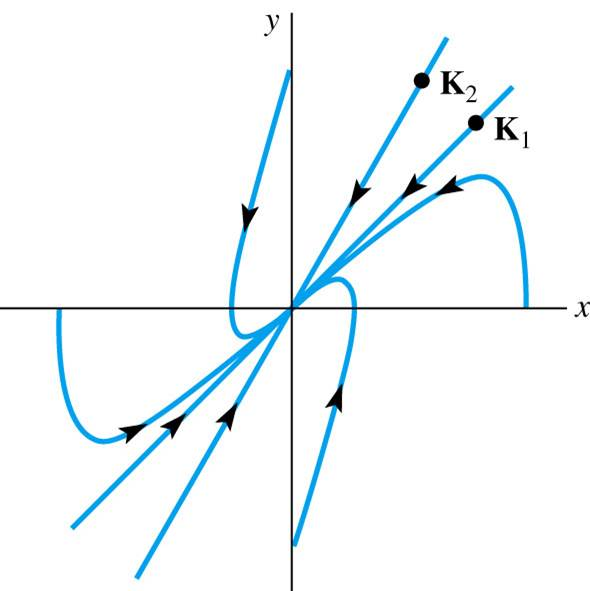
\includegraphics[scale=0.5]{nodoestable}
\caption{Nodo estable}
\end{figure}

\item[Nodo inestable]
Si ambos autovalores son positivos, la solución se aleja del orígen.
Las trayectorias de las soluciones son asintóticas a los autovalores de la matriz de coeficientes $A$, excepto las soluciones con condiciones iniciales que pertenecen a las direcciones propias, entonces el sistema evoluciona sobre ellas.
%
\begin{figure}
\centering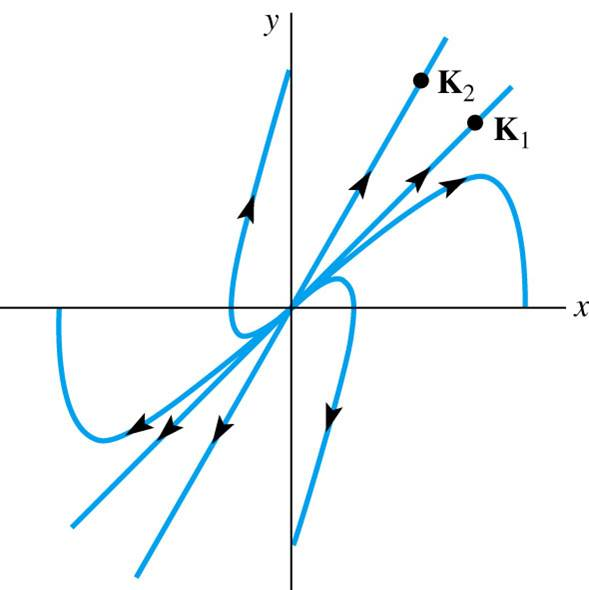
\includegraphics[scale=0.5]{nodoinestable}
\caption{Nodo inestable}
\end{figure}

\item[Punto silla]
Si los autovalores tienen signos opuestos, la solución se aleja del orígen asintóticamente a uno de los autovectores y se aproxima a él asintóticamente al otro, excepto las soluciones con condiciones iniciales que pertenecen a las direcciones propias, entonces el sistema evoluciona sobre ellas.
%
\begin{figure}
\centering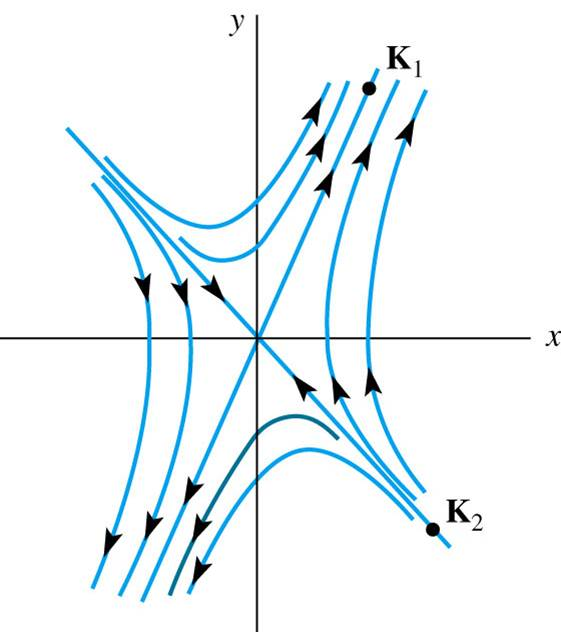
\includegraphics[scale=0.5]{silla}
\caption{Punto silla}
\end{figure}

\item[Nodos degenerados]
Aparecen en los casos en que los autovalores o autovectores sean iguales.
Para iguales autovalores, pueden generarse todas las trayectorias radiales por combinación lineal de los autovectores. La forma de la solución sería
\begin{equation}
X(t)=(c_1K_1+c_2+K_2)e^{\lambda t} \nonumber
\end{equation}
Si los autovalores son negativos, la solución se acerca al orígen en forma radial y el nodo resulta ser estable, de lo contrario será inestable.
\begin{figure}
\centering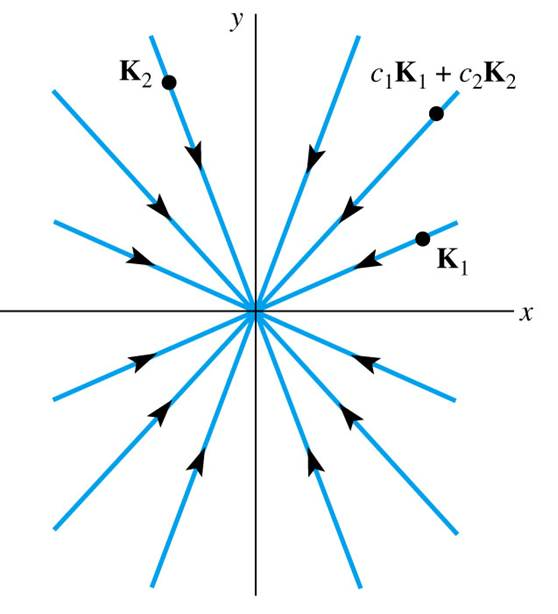
\includegraphics[scale=0.5]{nodoestabledegeneradounautovalor}
\caption{Nodo estable degenerado con autovalores negativos}
\end{figure}
Si además tenemos iguales autovectores, la forma de la solución sería
\begin{equation}
X(t)=(c_1K+tC_2K+c_2P)e^{\lambda t} \nonumber
\end{equation}
Si los autovalores son negativos, la solución se acerca al orígen y el nodo resulta ser estable, de lo contrario será inestable.
\begin{figure}
\centering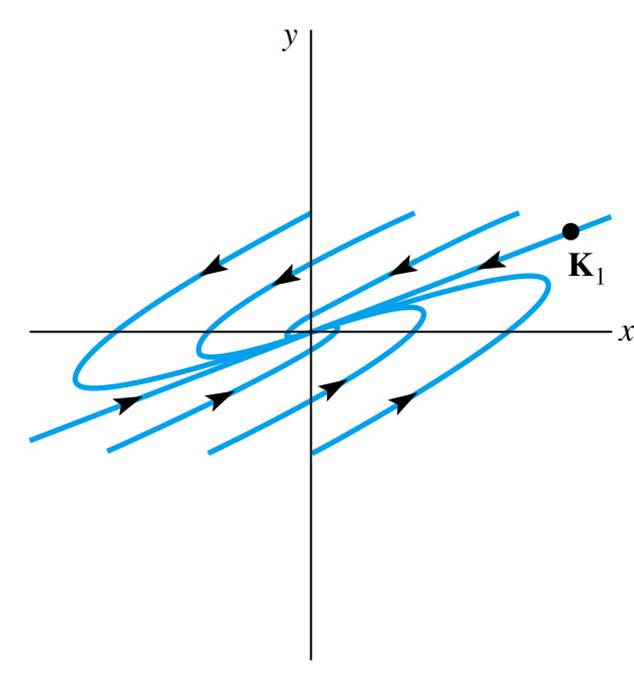
\includegraphics[scale=0.5]{nodoestabledegeneradounautovector}
\caption{Nodo estable degenerado con autovalores negativos y un solo autovector}
\end{figure}

\item[Centro]
Si los autovalores son imaginarios puros, la solución describe elipses concéntricas que pasan por el valor inicial.
\begin{figure}
\centering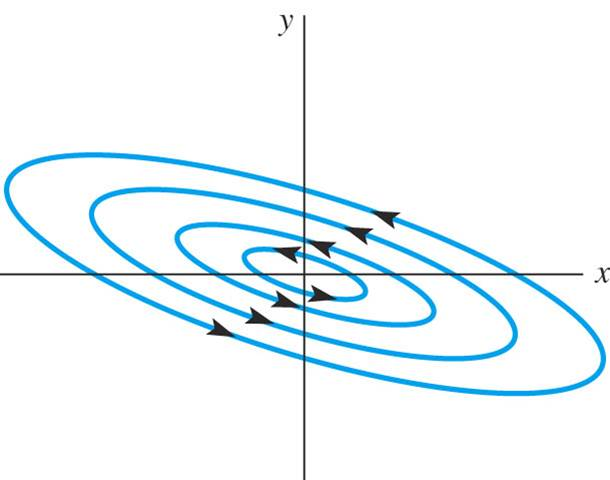
\includegraphics[scale=0.5]{centro}
\caption{Centro}
\end{figure}

\item[Foco estable]
Si los autovalores son complejos con parte real negativa, la solución es una combinación de los casos anteriores. Será periódica conforme su parte imaginaria y se aproximará a cero según su parte real.
%
\begin{figure}
\centering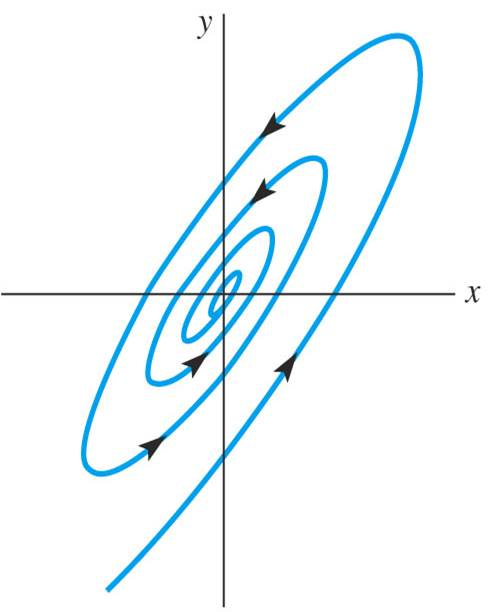
\includegraphics[scale=0.5]{focoestable}
\caption{Foco estable}
\end{figure}

\item[Foco inestable]
Si los autovalores son complejos, la solución será periódica conforme su parte imaginaria y se aproximará tenderá a infinito según su parte real.
%
\begin{figure}
\centering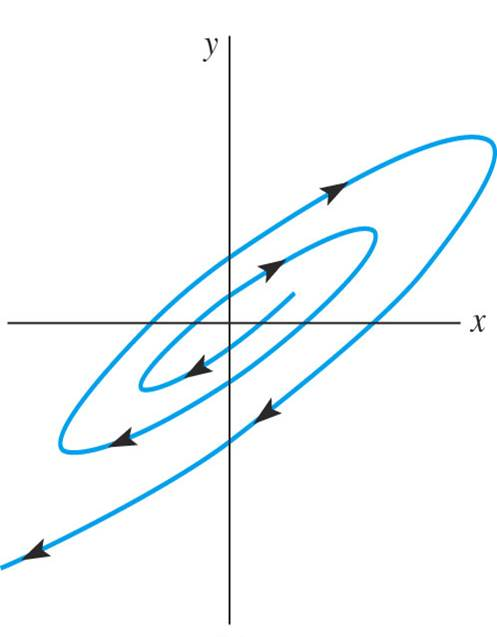
\includegraphics[scale=0.5]{focoinestable}
\caption{Foco inestable}
\end{figure}

\end{description}

Para cualquier  sistema de ED, primero se deben hallar todos los puntos críticos del sistema. Luego, se linealiza en torno a cada uno mediante el primer término de la serie de Taylor obteniendo tantos sistemas de ecuaciones como puntos críticos tenga el sistema.
Estos sistemas son válidos en un entorno suficientemente pequeño del punto crítico.

Por ejemplo, supongamos que se necesita trazar el diagrama de fase para el péndulo físico de la figura \ref{fig:pendulo}.
%
\begin{figure}[htpb]
	\centering
	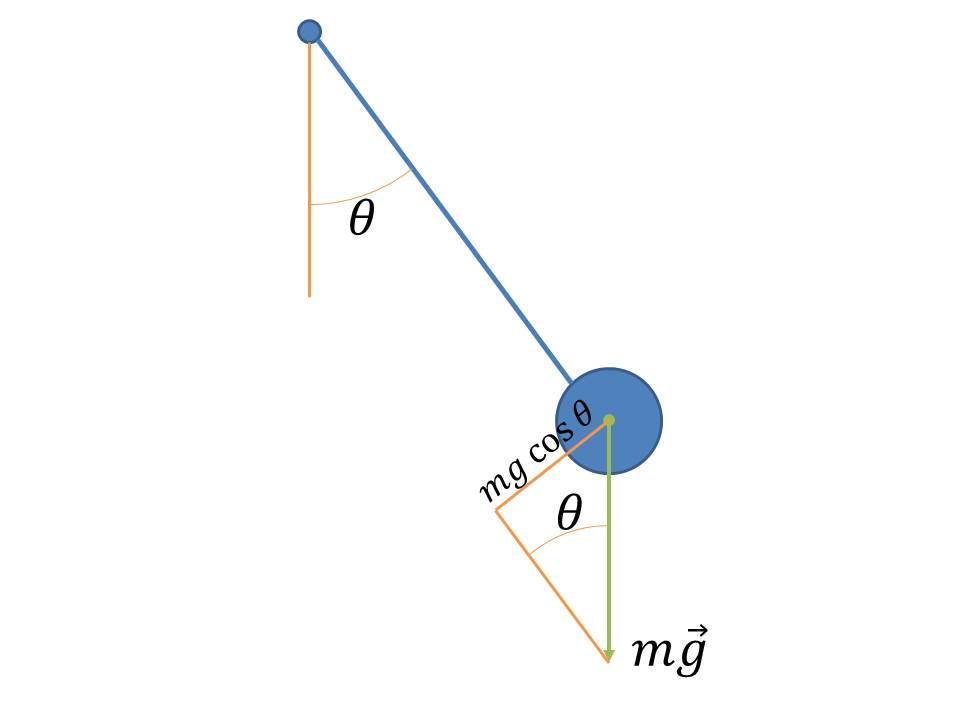
\includegraphics[width=.49\textwidth]{pendulo}
	\caption{Péndulo físico ideal.}
	\label{fig:pendulo}
\end{figure}

Primero hallamos la ecuación de la aceleración, según la figura, la componente tangencial de la gravedad es la que acelera al cuerpo.
Tomando como referencia positiva el sentido dextrógiro, queda
%
\begin{equation}
a=mg\cos\theta - \mu v \nonumber
\end{equation}
%
en donde $\mu$ es el coeficiente de roce viscoso con el aire y $v$ la velocidad. Pero como nos interesa la aceleración angular $\alpha$ y la velocidad angular $\omega$
%
\begin{equation}
\alpha=a/l; \qquad \omega=v/l \nonumber
\end{equation}
%
siendo $l$ la longitud de la cuerda.

La aceleración angular $\alpha$ es la derivada de la velocidad angular $\omega$ que a su vez es la derivada del ángulo $\theta$
%
\begin{equation}
\alpha = \omega' = \theta'' \nonumber
\end{equation}
%
entonces el sistema de ecuaciones queda
%
\begin{equation}
\left \{
\begin{array}{rcl}
\theta' &=& \omega\\
\omega' &=& \frac{mg}{l}\cos{\theta}-\frac{\mu}{l}\omega
\end{array}
\right. \nonumber
\end{equation}

Una vez planteado el sistema de ecuaciones, el primer paso es hallar los puntos críticos del sistema.
%
\begin{equation}
\left \{
\begin{array}{rcl}
0 &=& \omega\\
0 &=& \frac{mg}{l}\cos{\theta}-\frac{\mu}{l}\omega
\end{array}
\right.
\longrightarrow
\left \{
\begin{array}{rcl}
0 &=& \omega\\
\theta &=& (2n-1)\frac{\pi}{2} \qquad n\notin\mathbb{Z}
\end{array}
\right.
\nonumber
\end{equation}

Ahora estamos en condiciones de linealizar el sistema en torno de los puntos críticos.
% 
\begin{equation}
\left \{
\begin{array}{rcl}
\theta' &=& \omega\\
\omega' &=& \frac{\partial \left(\frac{mg}{l}\cos{\theta}\right)}{\partial\theta}\Big|_{\theta = (2n-1)\frac{\pi}{2}}\theta-\frac{\mu}{l}\omega
\end{array}
\right.
=
\left \{
\begin{array}{rcl}
\theta' &=& \omega\\
\omega' &=& -\frac{mg}{l}\sin(\theta)\Big|_{\theta = (2n-1)\frac{\pi}{2}}\theta-\frac{\mu}{l}\omega
\end{array}
\right.
\nonumber
\end{equation}

Según $n$ sea par (incluyendo el cero) o impar, la ecuación lineal que representa al sistema será diferente.

Si $n$ es par o cero
%
\begin{equation}
\left \{
\begin{array}{rcl}
\theta' &=& \omega\\
\omega' &=& \frac{mg}{l}\theta-\frac{\mu}{l}\omega
\end{array}
\right.
\longrightarrow
A=
\begin{pmatrix}
0 &1 \\
\frac{mg}{l} &-\frac{\mu}{l}
\end{pmatrix}
\nonumber
\end{equation}

\begin{equation}
det(A-\lambda I)= \;
\begin{vmatrix}
-\lambda &1 \\
\frac{mg}{l} &-\frac{\mu}{l}-\lambda
\end{vmatrix}
\nonumber
=\lambda^2+\frac{\mu}{l}\lambda-\frac{mg}{l}
\nonumber
\end{equation}
los autovalores son reales y de distinto signo (punto silla).

Si $n$ es impar
\begin{equation}
\left \{
\begin{array}{rcl}
\theta' &=& \omega\\
\omega' &=& -\frac{mg}{l}\theta-\frac{\mu}{l}\omega
\end{array}
\right. \nonumber
\end{equation}

\begin{equation}
det(A-\lambda I)= \;
\begin{vmatrix}
-\lambda &1 \\
-\frac{mg}{l} &-\frac{\mu}{l}-\lambda
\end{vmatrix}
\nonumber
=\lambda^2+\frac{\mu}{l}\lambda+\frac{mg}{l}\\
\nonumber
\end{equation}
los autovalores son complejos conjugados con parte real negativa (foco estable).

La resolución numérica en Matlab (figura \ref{fig:fase}, muestra las soluciones al sistema elineal en el espacio de estados.
Puede verse que en los puntos críticos, la solución se aproxima a un foco o a un punto silla, según el valor de $n$.
%
\begin{figure}
\centering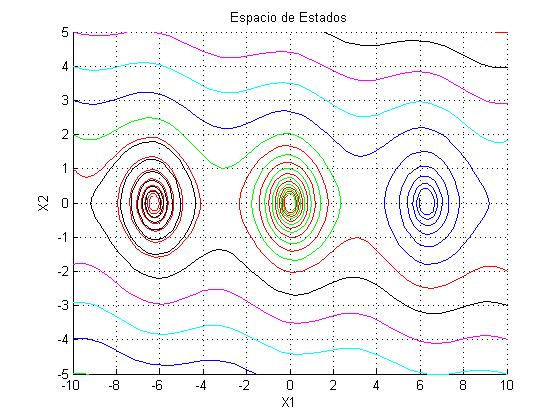
\includegraphics[scale=.7]{fase}
\caption{Diagrama de fase del péndulo físico real}
\label{fig:fase}
\end{figure}

\section{Sistemas caóticos}

Cuando se miden variables físicas, no es muy extraño encontrar que el plano de fases tiene un comportamiento similar al de la figura \ref{fig:Secuencia-OK_2}.
Puede verse que las trayectorias se cortan en el plano de fases, lo que indica que el sistema tiene un orden mayor que dos.
Otra observación que se puede hacer es que las trayectorias no se repiten, es decir que, aunque la oscilación persiste, no aparece un ciclo con trayectoria definida.
Esta última propiedad clasifica al sistema que se está midiendo como caótico.

\begin{figure}
\centering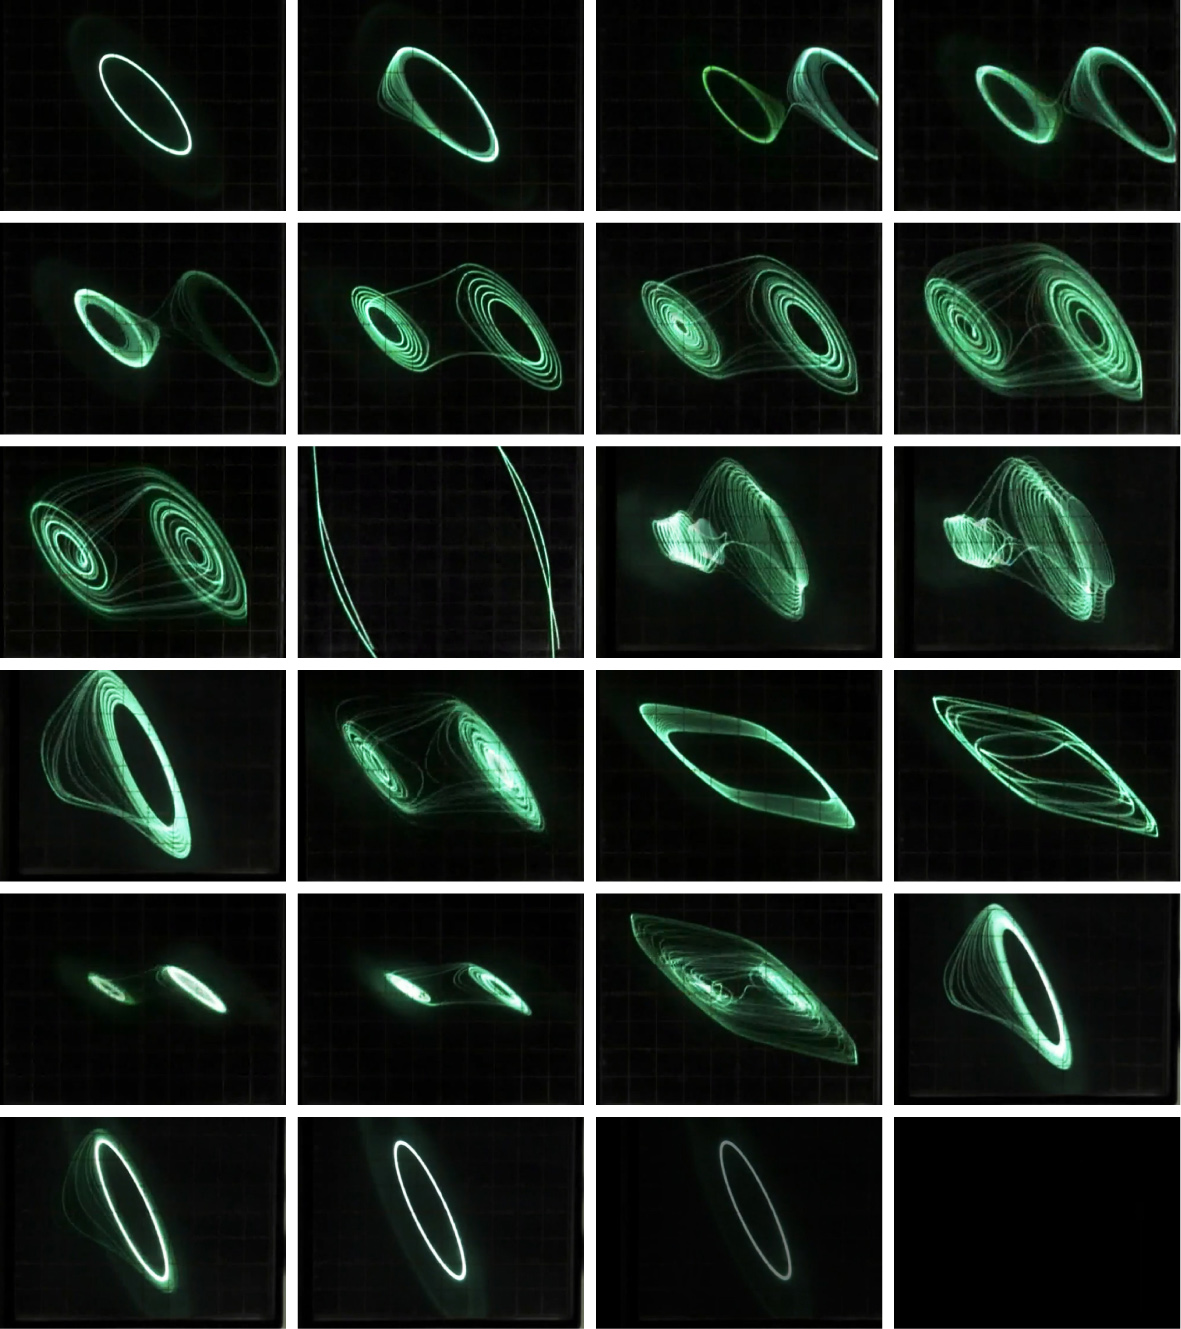
\includegraphics[width=0.8\textwidth]{Secuencia-OK_2}
\caption{Salidas de tensión de dos variables de un circuito oscilador}
\label{fig:Secuencia-OK_2}
\end{figure}

El teorema de existencia y unicidad de las soluciones a un sistema de ecuaciones garantiza que si f es continuamente diferenciable, los campos vectoriales sobre el espacio de fases son suaves y cada punto de este espacio tiene solución única.
La existencia de este teorema tiene un corolario importante: trayectorias diferentes nunca se intersectan.
Como consecuenciade esto, las trayectorias sobre el plano de fases quedan restringidas a: un nodo estable o inestable, centro, foco estable o inestable y puerto.
Entonces queda claro que un sistema continuo con derivada continua debe tener dimensión mayor o igual a tres para que pueda ser caótico, además, la trayectoria en el espacio de fases debe ocupar un dominio restringido.

Para describir analíticamente el comportamiento de este tipo de sistemas en torno a ciertos puntos de interés podemos hacer uso del álgebra lineal.
Lo que sigue son tres ejemplos de aplicaciones para atractores caóticos.

El primer y más común ejemplo es el sistema de Lorenz, que está descrito por el siguiente sistema de ecuaciones diferenciales \cite{Lorenz1963}
\begin{equation}\label{eq:lorenz}
\left \{
\begin{array}{rcl}
x_1' &=& \sigma (x_1-x_2)\\
x_2' &=& -x_1x_3+\rho x_3-x_2\\
x_3' &=& x_1x_2-\beta x_3
\end{array}
\right.
\end{equation}

El sistema de Lorenz tiene tres puntos de equilibrio, $E$, $E^+$ y $E^-$: el primer punto de equilibrio $E$ está situado en el origen (0,0,0) y los otros dos tienen respectivamente como coordenadas,
\begin{equation}
(x_1^\pm,x_2^\pm,x_3)=\left(\pm \sqrt{\beta(\rho-1)},\pm \sqrt{\beta(\rho-1)},\rho - 1\right) \nonumber
\end{equation}
El comportamiento físico interesante de este sistema ocurre cuando variamos el parámetro de control $\rho$.
Cuando $\rho<1$, todas las órbitas del campo vectorial dado por \ref{eq:lorenz} tienden al punto fijo situado en el origen.
A medida que se va incrementando más allá de la unidad, el origen pasa a ser inestable dando lugar a dos puntos fijos, estables, y simétricos $E^+$ y $E^-$. Para todo $\rho<1$, la geometría del comportamiento asintótico del sistema es la misma ya que todas las condiciones iniciales tienden al origen E.

Para $\rho>1$, se observan dos comportamientos.
El primero, asociado a valores de $\rho$ menores que un cierto valor de humbral $\rho_h=(\sigma(\sigma+\beta)+3\sigma)/(\sigma-\beta-1)$ , valor para el cual los puntos de equilibrio $E^+$ y $E^-$ pierden su estabilidad.
Dentro de este rango de valores del parámetro todas las órbitas terminan en uno de los dos puntos de equilibrio dependiendo de las condiciones iniciales.

Cuando $\rho>\rho_h$, la situación cambia drásticamente.
Los dos puntos fijos    pasan a ser inestables y nuevos comportamientos pueden surgir.
Para estudiar estos comportamientos se considera el análisis dinámico del sistema \ref{eq:lorenz}. 
La linealización del sistema \ref{eq:lorenz} en la proximidad del origen nos proporciona los siguientes autovalores:

\begin{equation}
\lambda = -\beta;\\
\lambda_\pm = \frac{1}{2} \left(-(\sigma+1) \pm \sqrt{(\sigma+1)^2+4\sigma(\rho-1)} \right) \nonumber
\end{equation}
 asociados a la matriz Jacobiana
 
\begin{equation}
\begin{pmatrix}
-\sigma &\sigma &0 \\
\rho &-1 &0 \\
0 &0 &-\beta
\end{pmatrix}
\nonumber
\end{equation}

Los autovalores  $\lambda$ y $\lambda_-$ son siempre negativos; el autovalor $\lambda_+$ cambia de negativo a positivo cuando $\rho$ pasa por el valor 1.

De modo similar, la linealización del sistema \ref{eq:lorenz} en la proximidad del punto de equilibrio $E^+$ nos proporciona los siguientes autovalores:
\begin{equation}
\lambda^3+\lambda^2(\sigma+\beta+1)+\lambda\beta(\sigma+\rho)+2\sigma\beta(\rho-1)=0 \nonumber
\end{equation}
asociados a la matriz Jacobiana
\begin{equation}
\begin{pmatrix}
-\sigma &\sigma &0 \\
\rho-x_3 &-1 &-x_1 \\
x_2 &x_1 &-\beta
\end{pmatrix}
\nonumber
\end{equation}
tiene un autovalor real negativo $\lambda$ combinado con dos autovalores imaginarios puros, $\lambda_\pm = \pm j \alpha$, si $\rho < \rho_h$

La linealización del sistema \ref{eq:lorenz} en la proximidad del punto de equilibrio $E^+$ es un problema simétrico a este.

En la figura \ref{fig:lorenz} pueden verse la evolución de las soluciones al sistema de lorenz.
%
\begin{figure}
\centering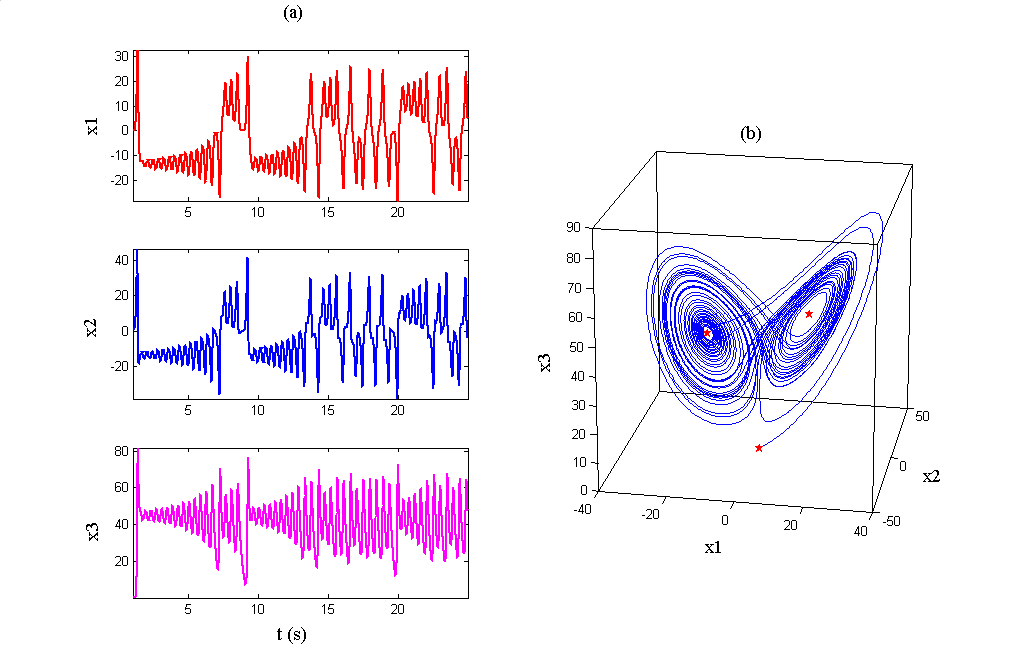
\includegraphics[scale=.4]{lorenz}
\caption{(a) Evolución temporal de las tres variables del sistema de Lorenz.(b) Disposición de sus puntos de equilibrio (estrellas rojas) con respecto a su atractor en el espacio de estados.}
\label{fig:lorenz}
\end{figure}

El sistema de Rössler está descrito por el siguiente sistema de ecuaciones diferenciales
\begin{equation}\label{eq:rossler}
\left \{
\begin{array}{rcl}
x_1' &=& x_2-x_3\\
x_2' &=& x_1x_3+ax_2\\
x_3' &=& b+(x_1+c)x_3
\end{array}
\right.
\end{equation}

Este sistema tiene dos puntos de equilibrio, $E^+$ y $E^-$ que existen solo cuando $\Delta=c^2-4ab>0$ y cuyas coordenadas están dadas respectivamente por,
\begin{equation}
(x_1^\pm,x_2^\pm,x_3^\pm)=\left( \frac{1}{2} (c \pm \sqrt{\Delta}),-\frac{1}{2a} (c \pm \sqrt{\Delta}),\frac{1}{2a} (c \pm \sqrt{\Delta})\right) \nonumber
\end{equation}
 
La linealización del sistema \ref{eq:rossler} en la proximidad de los puntos de equilibrio proporciona los siguientes autovalores:

\begin{equation}
a \lambda^3 - \lambda^2 a (x_1-c)-\lambda(x_3-1)+ax_3+(x_1-c)=0 \nonumber
\end{equation}
 asociados a la matriz Jacobiana
 
\begin{equation}
\begin{pmatrix}
0 &\-1 &-1 \\
1 &a &0 \\
x_3^\pm &0 &x_1^\pm-c
\end{pmatrix}
\nonumber
\end{equation}
de donde se deduce que fijando los parámetros $a$ y $b$ y variando $c$ nos encontramos con dos escenarios diferentes, podemos tener un autovalor real negativo y dos complejos conjugados con parte real positiva, o un autovalor real negativo y dos complejos conjugados con parte real negativa.
Para valores pequeños de c, el atractor de Rössler consiste en una órbita periódica o ciclo límite que tiene un sólo mínimo local.
A medida que vamos incrementando el parámetro c, el ciclo límite va duplicando su periodo y como consecuencia, sus mínimos locales hasta alcanzar un límite en el cual las trayectorias nunca se repiten lo que corresponde al atractor caótico de Rössler. 

En la figura \ref{fig:rossler_parametro} pueden verse la evolución de las $x_1$ y $x_2$ al sistema de Rössler para distintos valores del parámetro $c$.
En la figura \ref{fig:rossler}, la evolución de las tres variables para un parámetro fijo.
%
\begin{figure}
\centering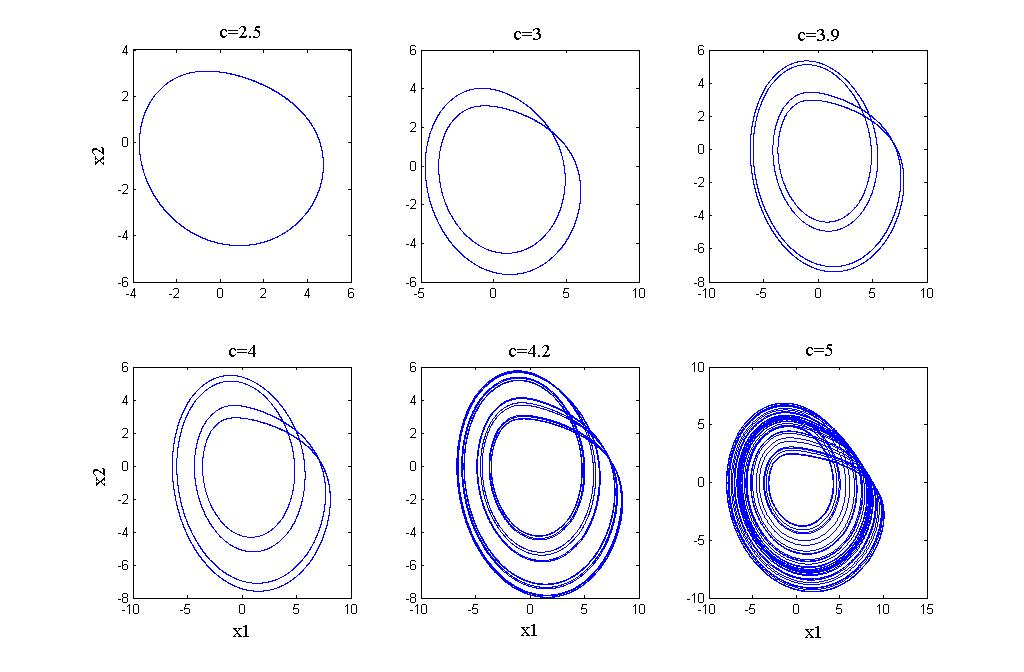
\includegraphics[scale=.5]{rossler_parametro}
\caption{Proyecciones del atractor de Rössler en el plano  para diferentes valores del parámetro c.}
\label{fig:rossler_parametro}
\end{figure}
%
\begin{figure}
\centering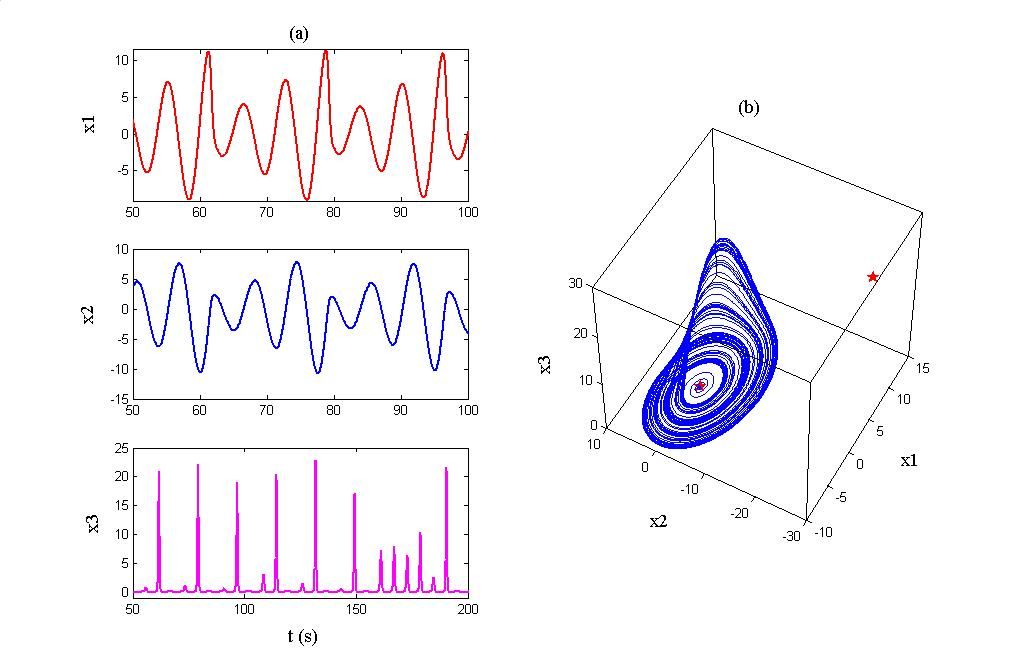
\includegraphics[scale=.5]{rossler}
\caption{(a) Evolución temporal de las tres variables del sistema de Rössler. (b) Disposición de sus puntos de equilibrio (estrellas rojas) con respecto a su atractor en el espacio de estados.}
\label{fig:rossler}
\end{figure}

El sistema de Chua está descrito por el siguiente sistema de ecuaciones diferenciales
\begin{equation}\label{eq:chua}
\left \{
\begin{array}{rcl}
x_1' &=& \alpha x_2- \alpha x_1^3- \alpha c x_1\\
x_2' &=& x_1 + x_3 - x_2\\
x_3' &=& -\beta x_2
\end{array}
\right.
\end{equation}

Tiene tres puntos de equilibrio, $E$, $E^+$ y $E^-$: el primer punto de equilibrio $E$ está situado en el origen (0,0,0) y los otros dos tienen respectivamente como coordenadas,
\begin{equation}
(x_1^\pm,x_2^\pm,x_3)=\left(\pm \sqrt{-c}, 0,\pm \sqrt{-c}\right) \nonumber
\end{equation}
Los puntos de equilibrio existen sólo para valores positivos del parámetro c.

La linealización del sistema \ref{eq:chua} en la proximidad de los puntos de equilibrio proporciona los siguientes autovalores:

\begin{equation}
\lambda^3 + \lambda^2 \alpha (\alpha c+1)+\lambda(\alpha c-\alpha+\beta)+ax_3+\alpha\beta c=0 \nonumber
\end{equation}
asociados a la matriz Jacobiana
\begin{equation}
\begin{pmatrix}
-\alpha c &\alpha &0 \\
1 &-1 &1 \\
0 &-\beta &0
\end{pmatrix}
\nonumber
\end{equation}
donde podemos detectar un punto de bifurcación para $\alpha=0$ en el cual el autovalor real negativo pasa a ser positivo provocando la inestabilidad del punto de equilibrio $E$ que permanece inestable para una amplia gama de valores del parámetro $\alpha$.

En la figura \ref{fig:chua}, puede verse la evolución de las tres variables de estado para este sistema.
%
\begin{figure}
\centering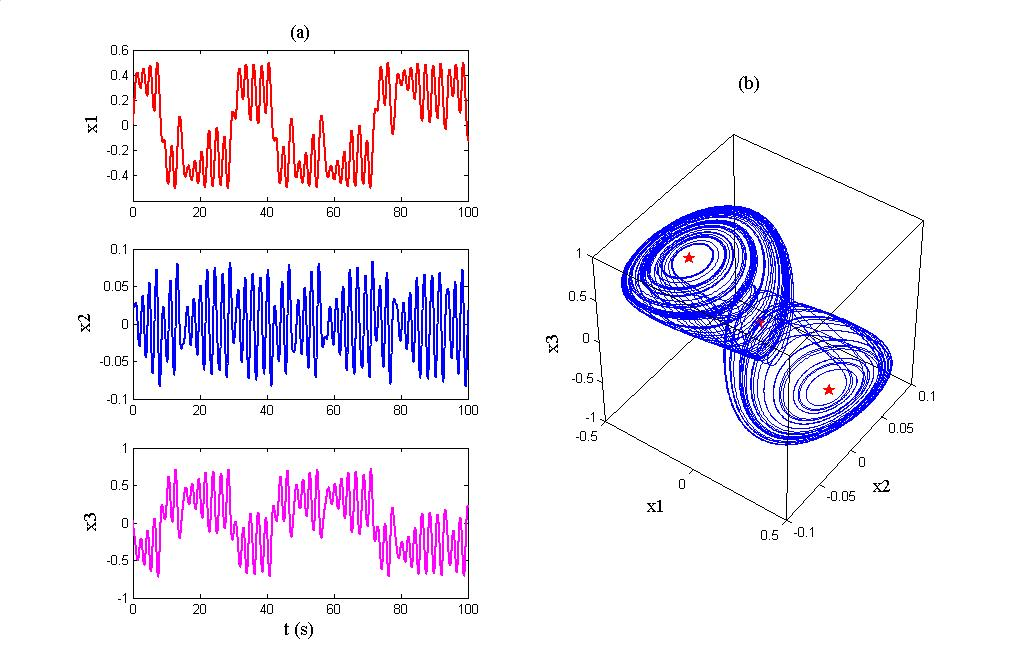
\includegraphics[scale=.5]{chua}
\caption{(a) Evolución temporal de las tres variables del sistema de Chua. (b) Disposición de sus puntos de equilibrio (estrellas rojas) con respecto a su atractor en el espacio de estados.}
\label{fig:chua}
\end{figure}

\section{Mapas caóticos}

¡¡¡¡¡¡¡¡¡¡¡¡¡¡¡¡¡¡¡Hablar de mapas como Logístico, tent, etc..!!!!!!!!!!!!!!!!!!!!

\subsection{Mapas cuadráticos bidimensionales}
\label{ssecQMaps}

La familia de mapas cuadráticos bidimensionales que estudiamos aquí es modelada por un par de ecuaciones cuadráticas acopladas:
%
\begin{equation}\label{eq:mapaSprott}
\left\{\begin{aligned}
x_{n+1}&=a_1+a_2 x_n+a_3 x_n^2+a_4 x_n y_n+a_5 y_n+a_6 y_n^2\\
y_{n+1}&=a_7+a_8 x_n+a_9 x_n^2+a_{10} x_n y_n+a_{11} y_n+a_{12} y_n^2
\end{aligned}
\right.
\end{equation}
%
donde $\{x, y\}$ son las variables de estado y $A = \{a_i, i = 1, \dots, 12 \}$ son los parámetros.
La principal característica de este sistema es que presenta múltiples atractores caóticos en función del punto seleccionado en el espacio del parámetros.
El espacio de parámetros de $12D$ generado por los coeficientes $A$ es muy difícil de explorar.

Las razones para estudiar este sistema en particular son dobles:
%
\begin{enumerate}
	\item Usando la aritmética de punto flotante con un barrido automático de parámetros $a_i$ y una gran cantidad de puntos en el espacio del parámetro (alrededor de $6\cdot10 ^ {16}$), Sprott pudo detectar varios atractores en régimen caótico permanente.
	Es decir, tienen la característica de modificar su atractor según los valores que tomen sus 12 coeficientes reales.
	Él también encontró una relación entre la dimensión de correlación y los exponentes de Lyapunov, con su estética visual, un tema interesante para la generación automática de arte.
	\item Es posible emplear estos atractores en una amplia variedad de aplicaciones electrónicas, como la generación de nuevos sistemas de encriptación, ya sea reemplazando el S-box en AES \cite{Ahmad2013, Hussain2013}, o incluso desarrollando nuevos algoritmos \cite{Machado2004, Smaoui2009}.
\end{enumerate}

Tres de estos atractores caóticos se muestran juntos en la figura \ref{fig:atractoresQMaps}.
Sus juegos de parámetros $A_i$ son:	
%
\begin{eqnarray}
A_1&=\{-0.7,-0.4,0.5,-1.0,-0.9,-0.8,0.5,0.5,0.3,0.9,-0.1,-0.9\},\nonumber\\
A_2&=\{-0.6,-0.1,1.1,0.2,-0.8,0.6,-0.7,0.7,0.7,0.3,0.6,0.9\}, \nonumber\\
A_3&=\{ -0.1,0.8,-0.7,-1.1,1.1,-0.7,-0.4,0.6,-0.6,-0.3,1.2,0.6\}.\nonumber\\
\end{eqnarray}
%
Como se puede ver en la figura, es posible obtener salidas muy diferentes simplemente modificando el valor de los parámetros y manteniendo la estructura del sistema.
En una implementación electrónica, esto sería equivalente a poder variar la salida manteniendo la estructura del hardware y modificando los parámetros a través de, por ejemplo, una entrada.
%
\begin{figure}
	\centering
	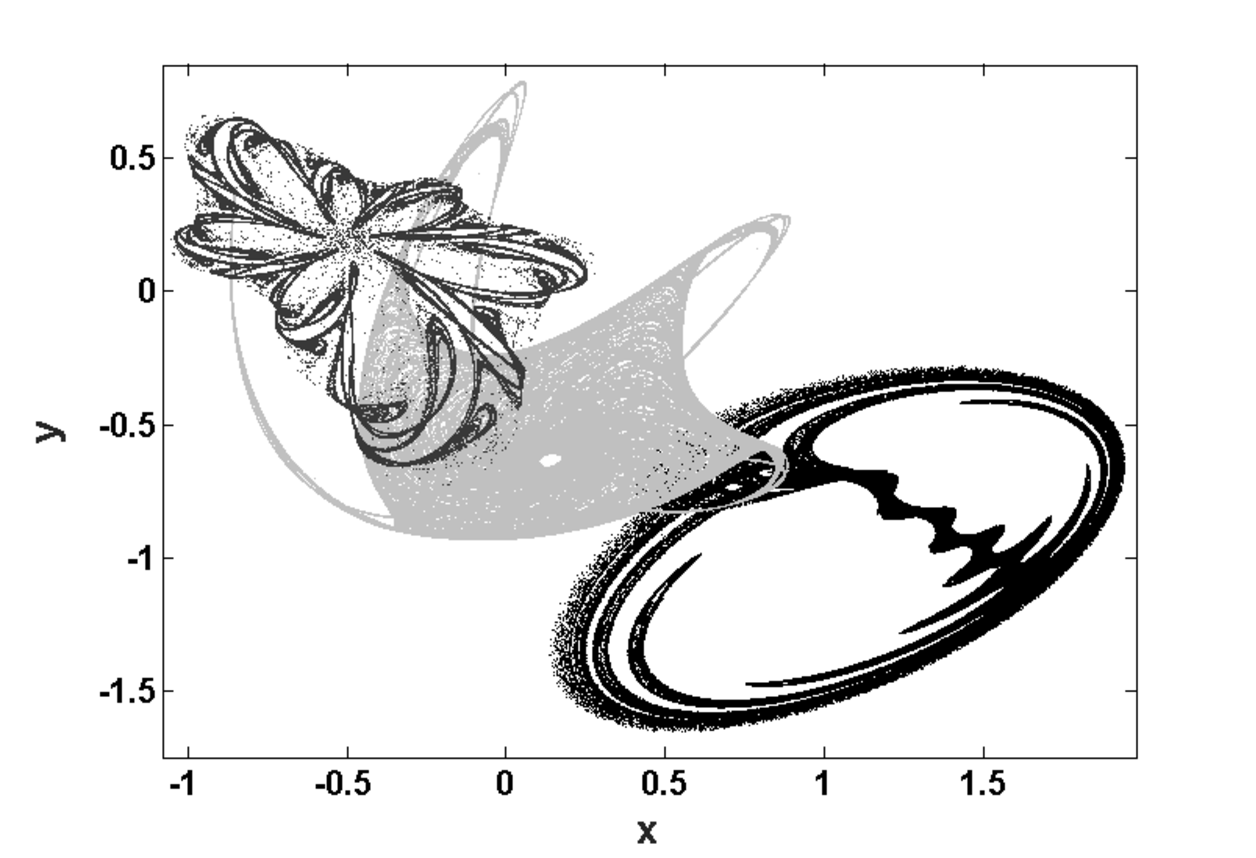
\includegraphics[width=1\columnwidth]{atractoreslindos}\\
	\caption{Tres atractores para tres juegos de parámetros distintos.}\label{fig:atractoresQMaps}
\end{figure}

Las figuras \ref{fig:atractores3592}.a a \ref{fig:atractores3592}.d muestran los mismos tres atractores $A_1$ a $A_3$ de la Fig. \ref{fig:atractoresQMaps} junto a un atractor con $A_4=\{-1,0.9,0.4,-0.2,-0.6,-0.5,0.4,0.7,0.3,-0.5,0.7,-0.8\}$, superpuestos con sus regiones de atracción (en gris).
Las áreas blancas de cada figura corresponden a aquellas condiciones iniciales que generan trayectorias divergentes del sistema (semillas inútiles con respecto a su uso como PRNG).	
%
\begin{figure}
	\centering
	\begin{subfigure}[b]{0.49\textwidth}
		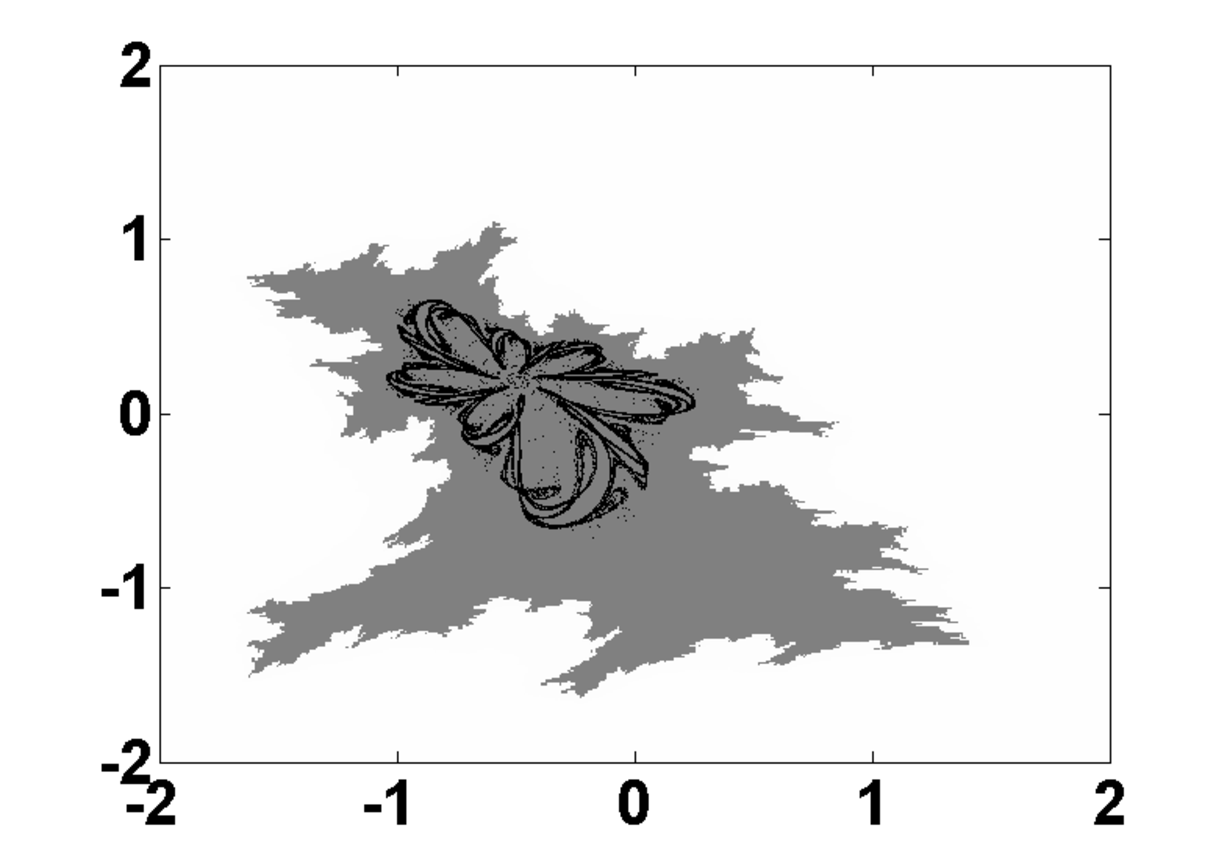
\includegraphics[width=\textwidth]{Atractor3_condominio}
		\caption{$\{a_i\}=A_1$.}
	\end{subfigure}
	\hfill 
	\begin{subfigure}[b]{0.49\textwidth}
		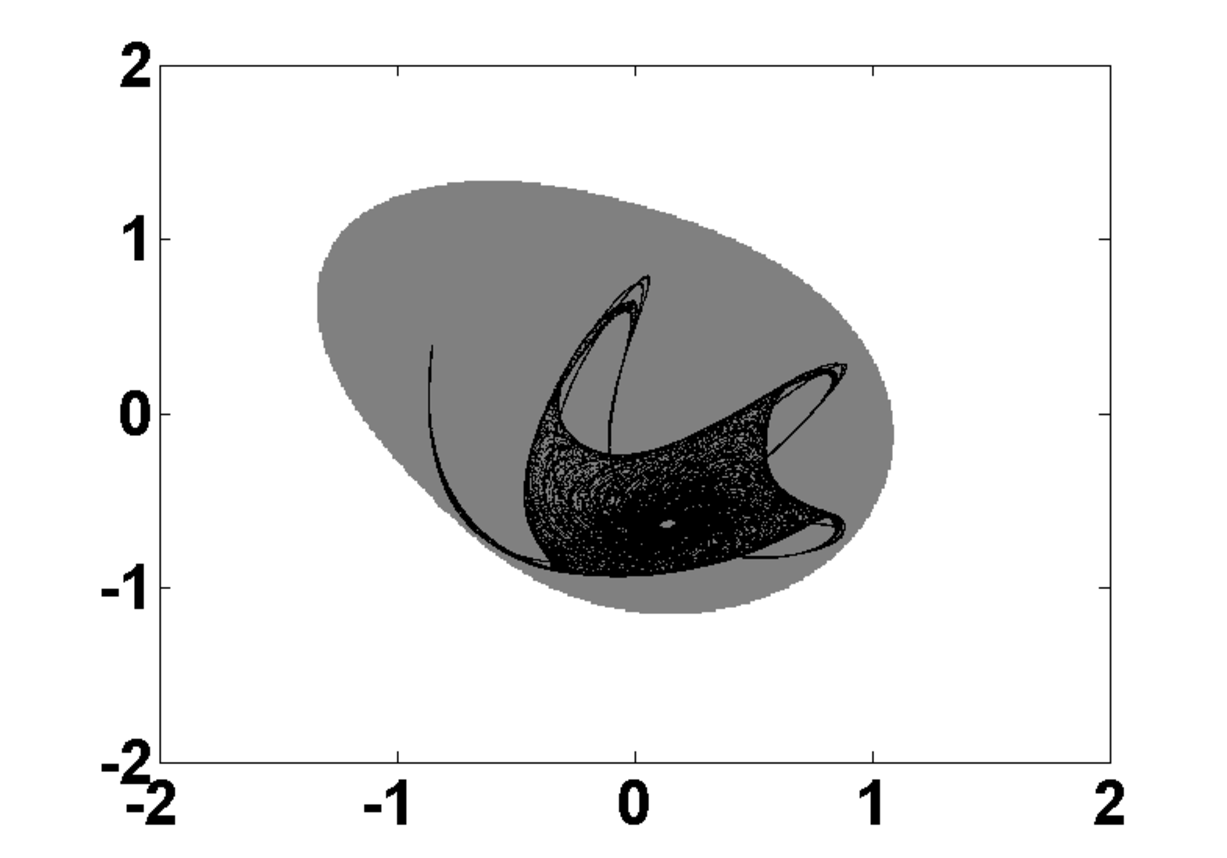
\includegraphics[width=\textwidth]{Atractor5_condminio}
		\caption{$\{a_i\}=A_2$.}
	\end{subfigure}
	\hfill 
	\begin{subfigure}[b]{0.49\textwidth}
		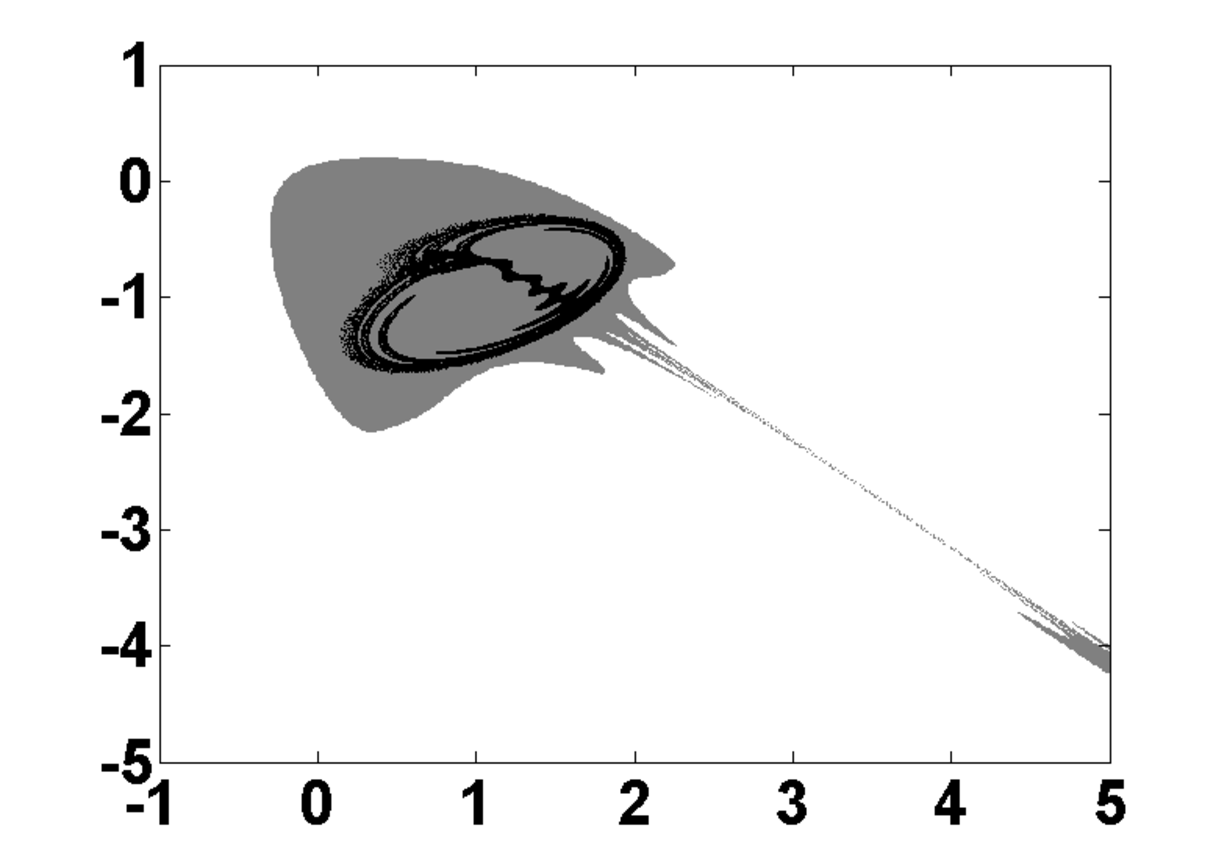
\includegraphics[width=\textwidth]{Atractor9_condominio}
		\caption{$\{a_i\}=A_3$.}
	\end{subfigure}
	\hfill  
	\begin{subfigure}[b]{0.49\textwidth}
		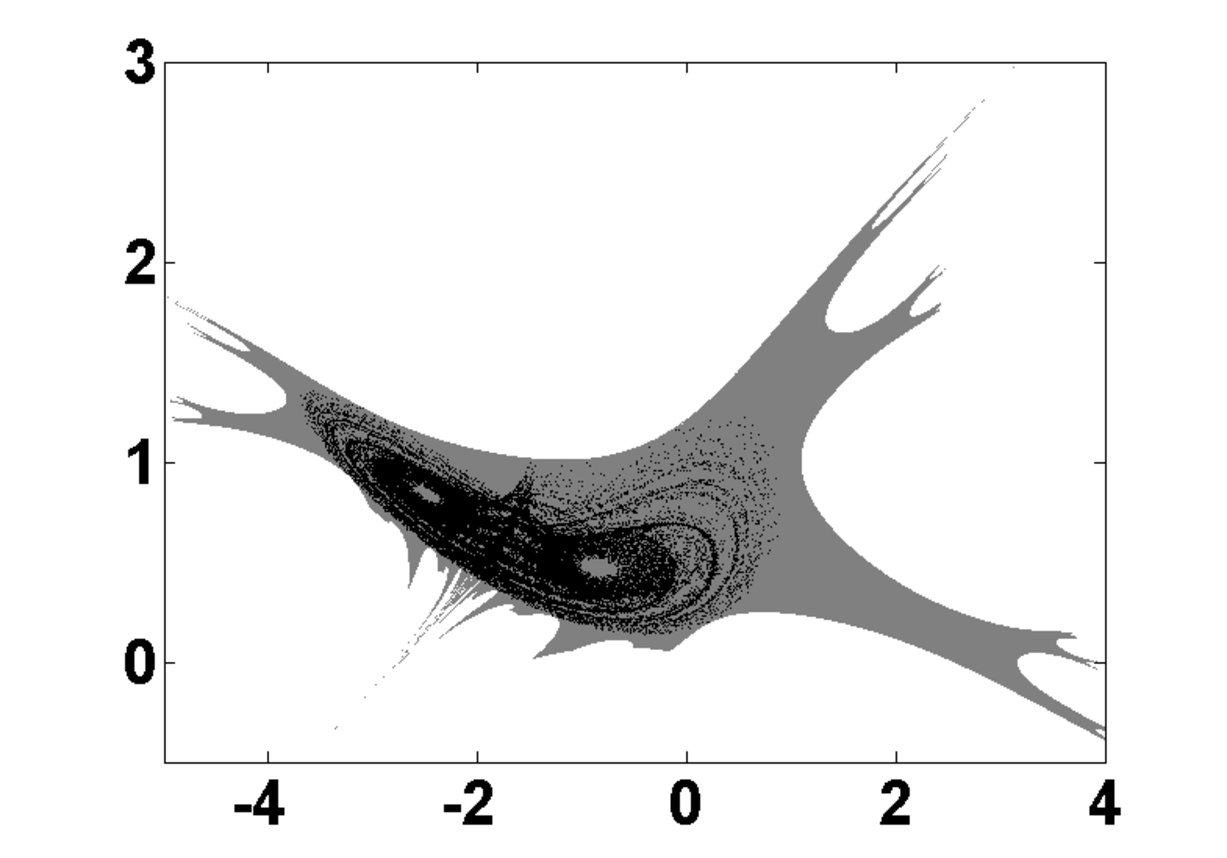
\includegraphics[width=\textwidth]{Atractor2_condominio}
		\caption{$\{a_i\}=A_4$.}
	\end{subfigure}
	\caption{Cuatro atractores caóticos y sus respectivos dominios de atracción.}
	\label{fig:atractores3592}
\end{figure}

\thispagestyle{empty}

\chapter{Cuantificadores de Aleatoriedad}

\section{Máximo Exponente de Lyapunov}
\label{sec:MLE}

El Máximo Exponente de Lyapunov (MLE) caracteriza que tan rápido se apartan dos trayectorias.
Si esta velocidad es exponencial, se dice que el sistema es caótico, por lo que este exponente es conocido como un detector de  ``caoticidad", \cite{strotgartz1994,Kantz1994,Sprott2003}.
Más adelante, el MLE fue utilizado en diversas aplicaciones de muy distintas áreas.
Sólo por mencionar alguna, en \cite{Ma2013} el MLE es usado para medir una señal muy débil en un gas ideal utilizando criterios caóticos.
En \cite{Bruijna2011}, se estudia si es posible predecir un cambio en la probabilidad de caída para un modelo simple de caminante humano a partir del $MLE$.

Los exponentes de Lyapunov son quantificadores que caracterizan como evoluciona la separación entre dos trayectorias \cite{Sprott2003}.
En general es bien conocido que el comportamiento caótico está principalmente caracterizado por los números de Lyapunov de la dinamica del sistema.
Si uno o mas números de Lyapunov es mayor que cero, entonces el sistema se comporta caóticamente, de otra forma el sistema es estable.

La distancia entre dos trayectorias cambia en $2^{MLE}$ por cada iteración, en promedio.
Si el $MLE<0$ las trayectorias se aproximan, esto puede deberse a un punto fijo.
Si el $MLE=0$ las trayectorias mantienen su distancia, esto puede deberse a un ciclo límite.
Si el $MLE>0$ la distancia entre las trayectorias es creciente, lo que es un indicador de caos.

Existe una forma no analítica de medir el $MLE$ si solo las entradas y las salidas de un sistema son accesibles.
El procedimiento es el siguiente: el sistema debe ser iniciado desde dos puntos cercanos en el plano de fase, llamémoslos $(x_a,y_a)$ y $(x_b,y_b)$.
A medida que el sistema es iterado se mide la distancia euclideana entre las dos trayectorias ($d_n$ en la muestra $n_{th}$) (eq. \ref{eq:D0D1}), y la trayectoria $b$ es relocalizada en cada iteración (eq. \ref{eq:reubicacion}) obteniendo los puntos $(x_{br},y_{br})$ para realimentar el sistema.
Entonces, el MLE puede ser calculado como se muestra en la ecuación \ref{eq:Lyapunov}.
El proceso puede verse en la Fig. \ref{fig:relocalizacion}.

\begin{eqnarray}\label{eq:D0D1}
d_{0(i-1)}&=& \sqrt{(x_{a(i-1)}-x_{br(i-1)})^2+(y_{a(i-1)}-y_{br(i-1)})^2}\nonumber\\
d_{1(i)}&=& \sqrt{(x_{a(i)}-x_{b(i)})^2+(y_{a(i)}-y_{b(i)})^2}\\
\nonumber
\end{eqnarray}

\begin{eqnarray}\label{eq:Lyapunov}
MLE &=& \frac{1}{n} \sum_{i=2}^{n} \log_2{\frac{d_{1(i)}}{d_{0(i-1)}}}
\end{eqnarray}

\begin{eqnarray}\label{eq:reubicacion}
x_{br(i)}&=& x_{a(i)}+(x_{b(i)}-x_{a(i)})d_{o(i-1)}/d_{1(i)} \nonumber\\
y_{br(i)}&=& y_{a(i)}+(y_{b(i)}-y_{a(i)})d_{o(i-1)}/d_{1(i)}
\end{eqnarray}

\begin{figure}
	\centering
	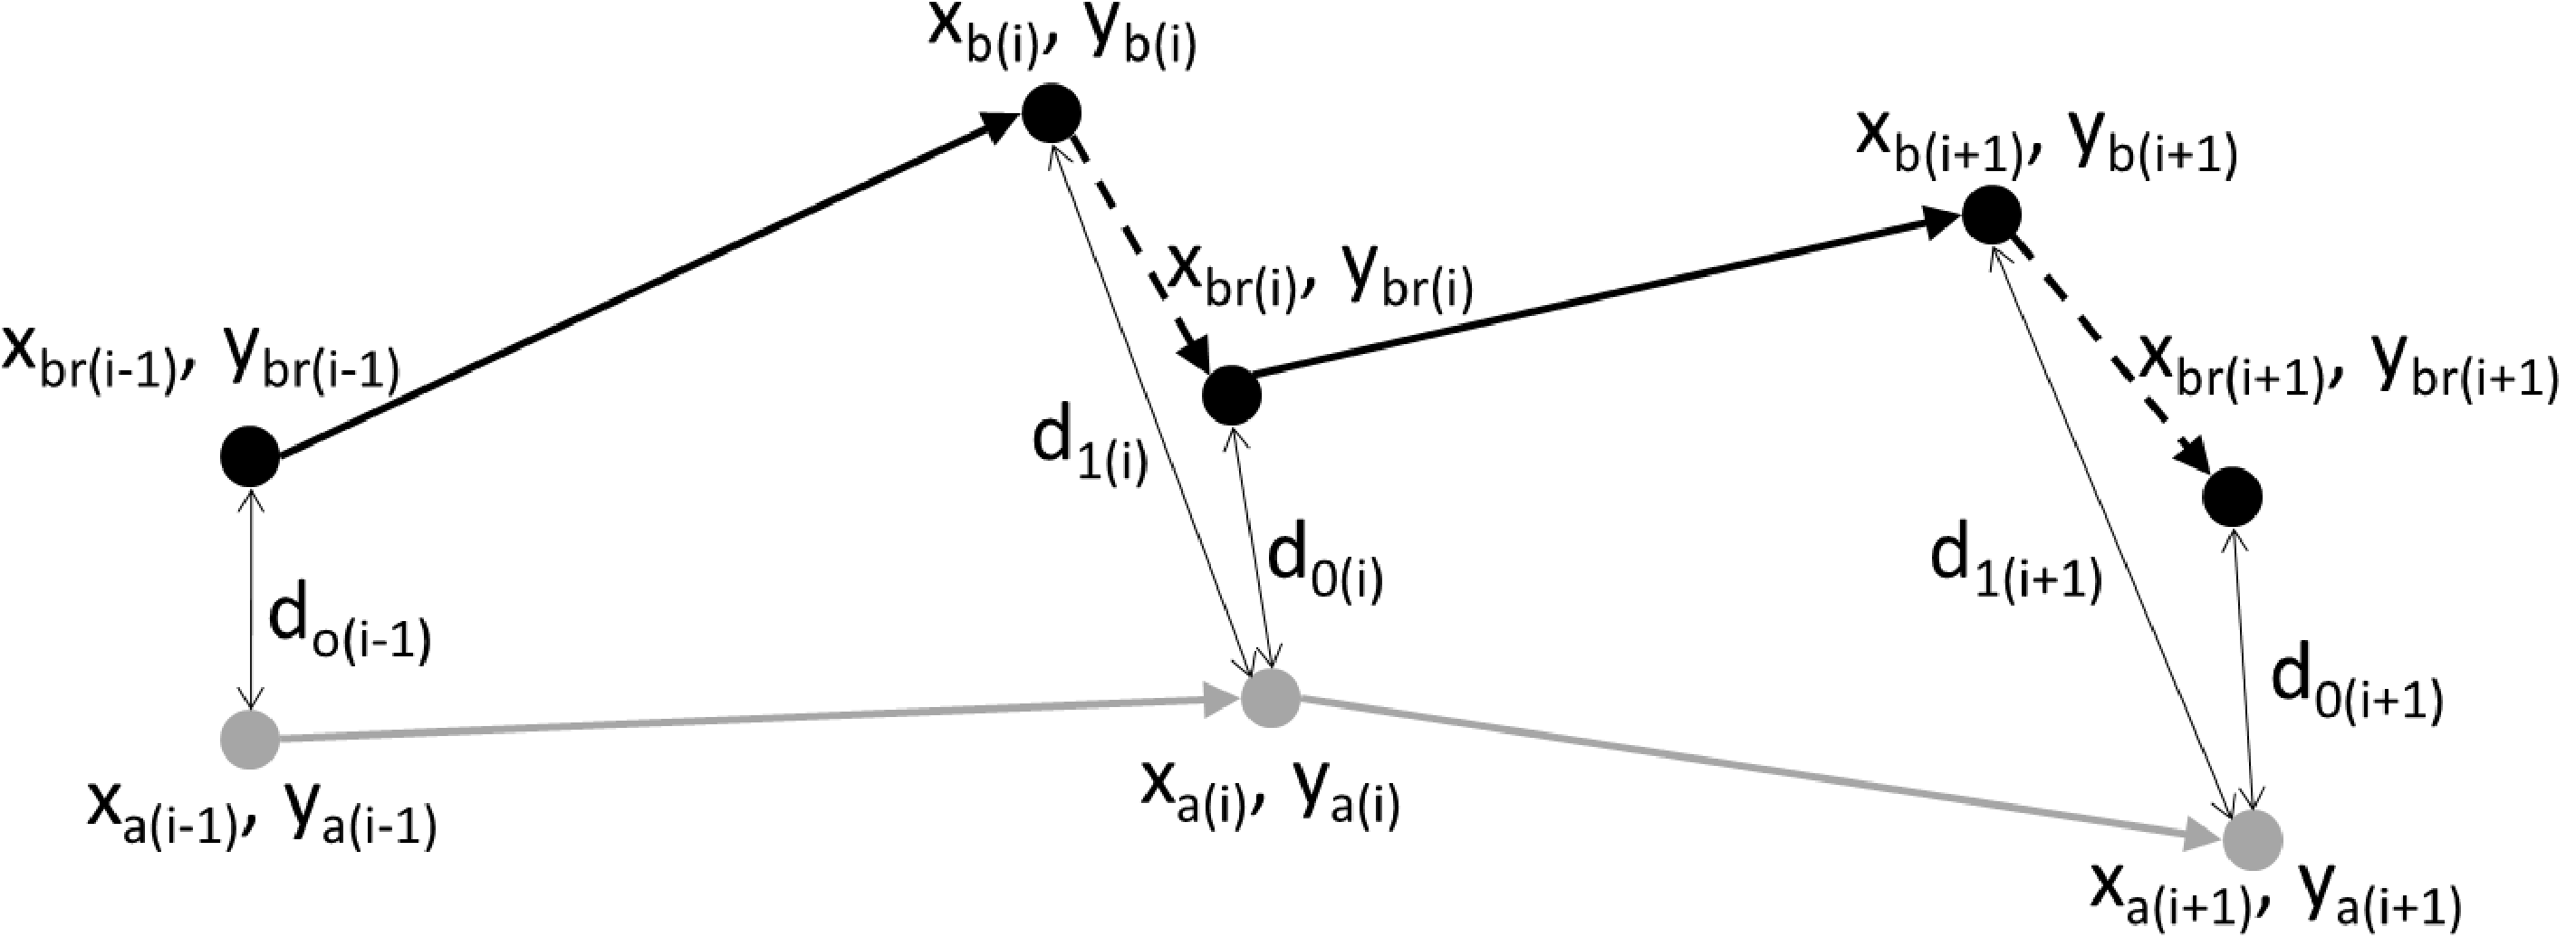
\includegraphics[width=1\columnwidth]{relocalizacion.pdf}\\
	\caption{Algoritmo para calcular el MLE.}\label{fig:relocalizacion}
\end{figure}


\subsection{Algoritmo evolutivo para la búsqueda de caos}

Se propuso emplear un método eurístico para buscar parámetros del sistema implementado de tal forma que se maximice la caoticidad de su salida.
Este algoritmo tiene la ventaja que realiza una búsqueda inteligente mediante el empleo de un algoritmo genético, lo que minimiza el tiempo de cómputo.

Un algoritmo evolutivo es un método de búsqueda dirigido basado en la probabilidad.
Un juego de entidades que representan posibles soluciones compite con otros, evolucionando en mejores soluciones \cite{Weise2009}.

Las entidades que representan posibles soluciones al problema son llamados \textit{cromosomas} y el grupo de cromosomas es llamados \textit{población inicial}.

Desde la población inicial, o los primeros padres, se genera un hijo mediante el cruce entre ellos.
Luego, ellos son mutados en forma aleatoria para crear la próxima generación.
Cada generación es comparada con la previa para descartar los ``peor adaptados" y así los coeficientes (cromosomas) mutan hacia los ``mejor adaptados".

Cuando se aplican estos algoritmos en funciones continuas, siempre convergen hacia el máximo local.
Sin embargo, si el espacio de coeficientes es fractal, existen áreas bien definidas en donde el la función objetivo es positiva, negativa, cero o no existente.
Este es el caso si la función a maximizar es el MLE y el espacio de exploración es el de parámetros.

\subsubsection{Resultados}

Para evaluar la viabilidad del método, se generó el siguiente algoritmo y se probó sobre el mapa logístico.

En la figura \ref{fig:diagramaflujo1} podemos ver el diagrama de flujo principal.
El bloque \textit{Evolution} fue descompuesto en otro sub-diagrama para simplificar la descripción.
Este segundo diagrama puede verse en la figura \ref{fig:diagramaflujo2}, esta surutina maneja la evolución de los parámetros.
%
\begin{figure}
	\centering
	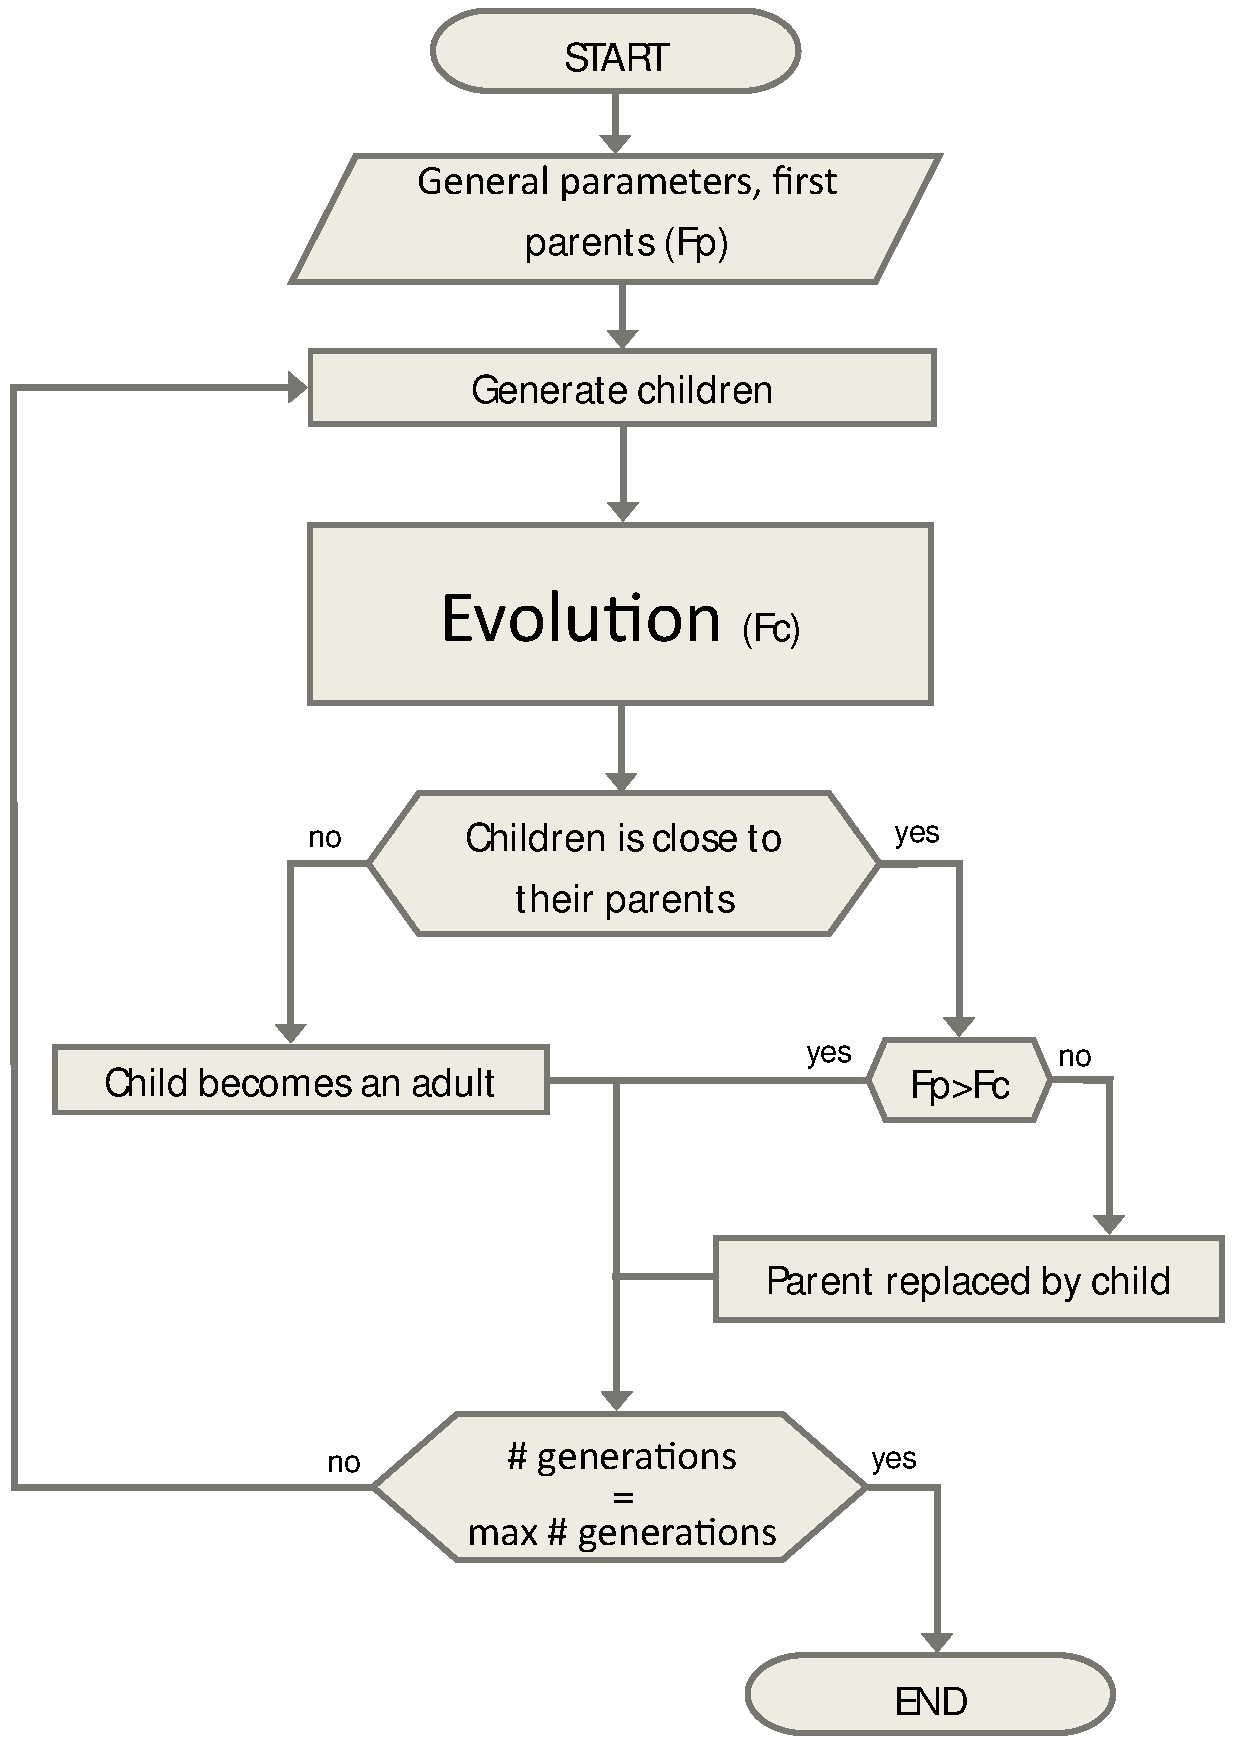
\includegraphics[width=0.9\columnwidth]{main_flowchart}\\
	\caption{Diagrama de flujo principal.}
	\label{fig:diagramaflujo1}
\end{figure}
%
\begin{figure}
	\centering
	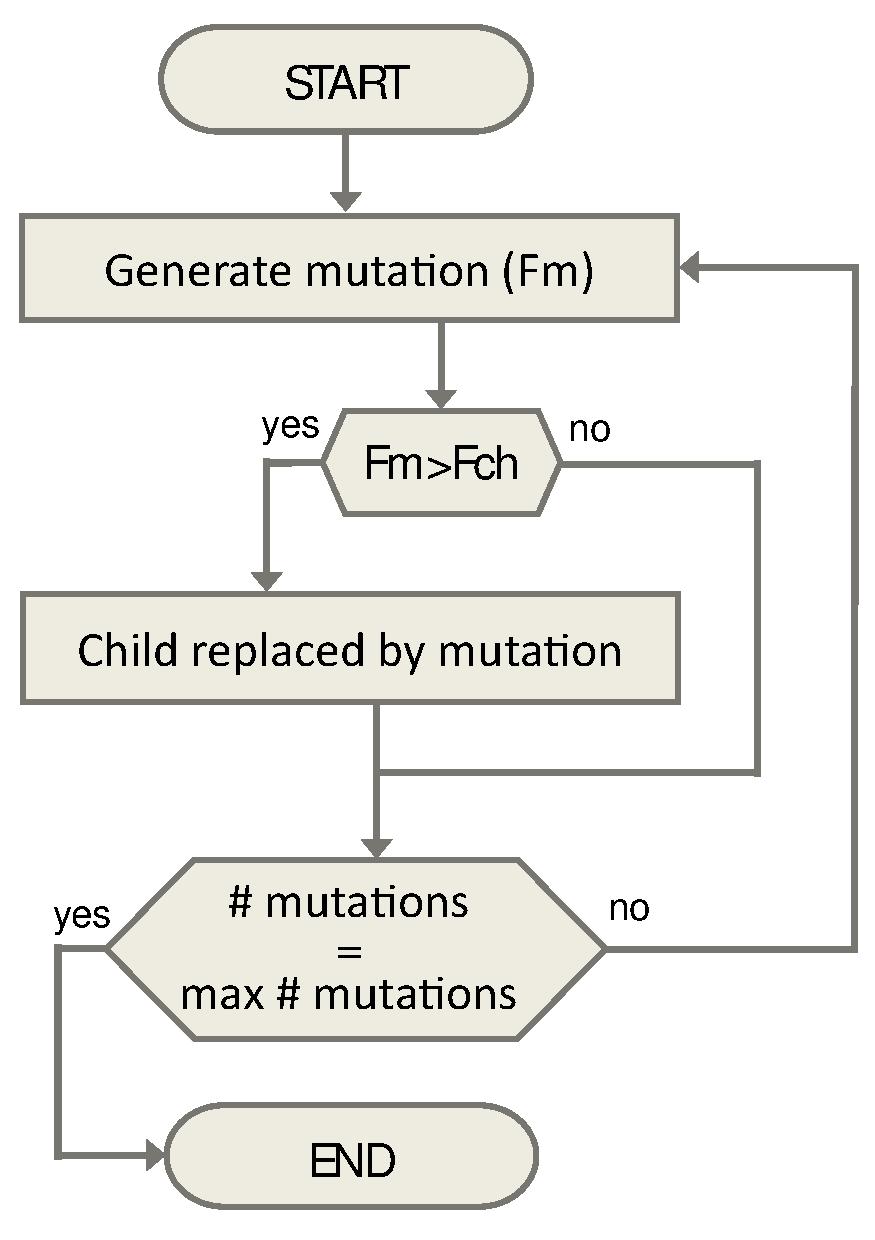
\includegraphics[width=0.56\columnwidth]{evolution_flowchart.pdf}\\
	\caption{Diagrama de flujo del bloque \textit{Evolution}.}\label{fig:diagramaflujo2}
\end{figure}

El algoritmo inicia con una inicialización general de parámetros como el número máximo de generaciones $max\_gen$, el número máximo de mutaciones $max\_mut$ y el número máximo de cambios en cada mutación $max\_stem$.
Luego se definen los primeros dos padres, ellos definirán los márgenes de búsqueda.
Además se calcula su \textit{fitness function} $Fp$.
A partir de este punto se itera la segunda generación, se elige en forma aleatoria un valor de parámetro $r$ con una distribución aleatoria entre los primeros dos padres, generando un nuevo hijo.
Luego este hijo entra en la subrutina \textit{Evolution} cuya salida es el valor de $r$ evolucionado y su correspondiente $Fc$.

Luego se evalúa si este hijo avolucionó muy cerca de sus padres o no.
Si la distancia entre ellos es más grande que el parámetro $max\_hop$, entonces este hijo es considerado como adulto, en caso contrario debe competir con su padre más cercano sobreviviendo el más apto.

Este proceso se repite hasta que se llega al máximo número de  generaciones $max\_gen$.
El grupo final de adultos es la solución al problema de buscar los máximos MLE locales.

La subrutina \textit{Evolution} de la figura \ref{fig:diagramaflujo2}) es un algoritmo muy simple basado en mutaciones.
El primer paso es generar una mutación del hijo con una probabilidad uniformemente distribuida entre $\pm max\_step$, tambien se calcula su \textit{fitness function} $Fm$, que se compara con la del individuo original $Fc$.
Entonces sobrevive el mejor adaptado para dar lugar a la siguiente mutación.
Este procedimiento se repute hasta que se llega al máximo número de mutaciones $max\_mut$.

Como resultado podemos ver el $MLE$ del mapa logístico en función de su único parámetro $r$ en la figura \ref{fig:resultadoAlgorithm}.
La línea contínua muestra el $MLE$ en pasos continuos de $r$, mientras que los puntos destacados son el resultado del algoritmo propuesto.
%
\begin{figure}
	\centering
	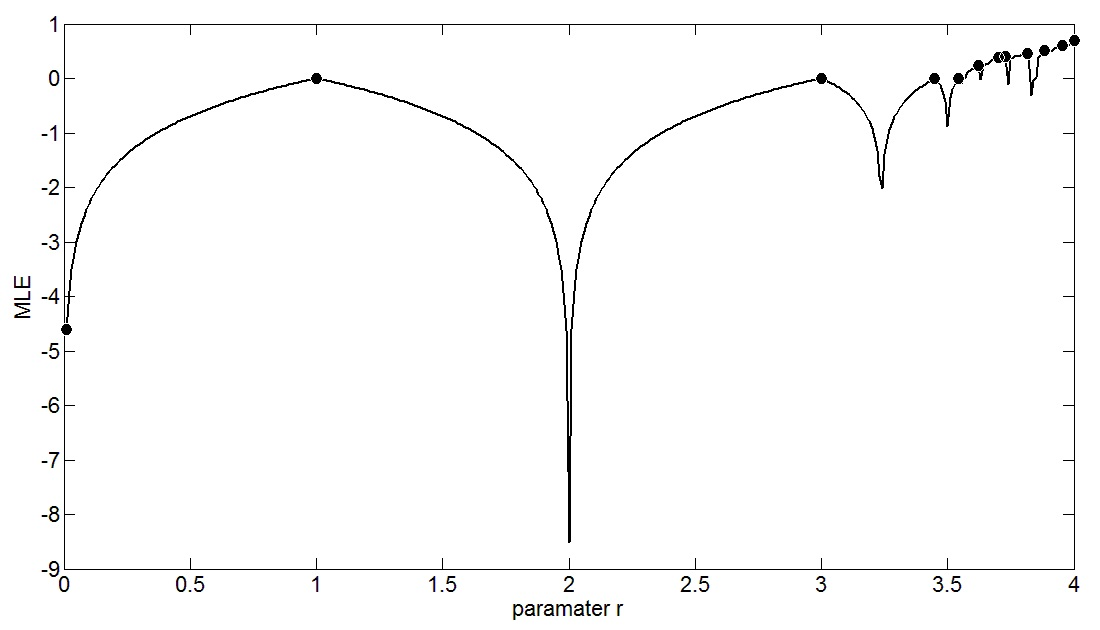
\includegraphics[width=1\columnwidth]{EvolutivoVSExaustivo.jpg}\\
	\caption{Resultados del algoritmo evolutivo para el mapa logístico, los puntos son los resultados del algoritmo.}\label{fig:resultadoAlgorithm}
\end{figure}

El bloque que calcula el $MLE$ fue sintetizado y verificado experimentalmente en un Altera CYCLONE III FPGA y los resultados de la compilación mostrados en la figura \ref{fig:compilacion}.
Los resultados del \textit{Timing Analysis} reportan que la máxima frecuancia es de $84.95MHz$.
El reporte de compilación muestra que la utilización de la lógica no excede el $20\%$, es decir un total de $20307$ de elementos lógicos, $54\%$ de los bits de memoria totales y $8\%$ de los multiplicadores embebidos.
%
\begin{figure}
	\centering
	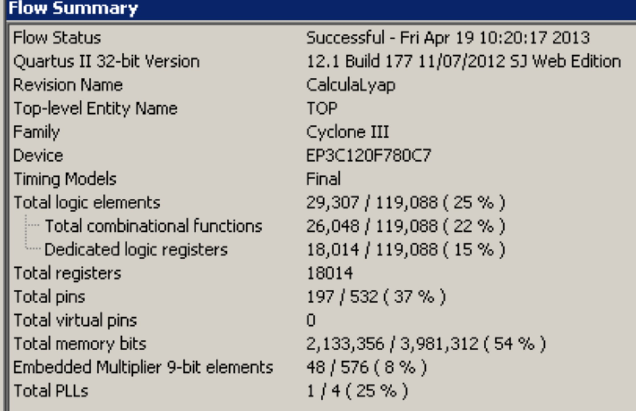
\includegraphics[width=1\columnwidth]{compilacion.pdf}\\
	\caption{Compilation report of the \textit{MLE} calculator.}\label{fig:compilacion}
\end{figure}

En la figura \ref{fig:st} se muestra la salida del Signal Tap.
La señal \textit{salida} es la suma de los $MLE$ luego de cada iteración.
La segunda señal llamada \textit{cuenta\_sal} corresponde a la sumatoria actual.
Finalmente, cada flanco descendente de la señal \textit{listoD1} indica que la salida es un dato válido.
La salida fué procesada con Matlab para obtener la curva mostrada en la figura\ref{fig:lyapu}.
El valor del MLE en la iteración $250000$ es $0.1415$, lo que es consistente con el MLE obtenido con Matlab.
%
\begin{figure*}
	\centering
	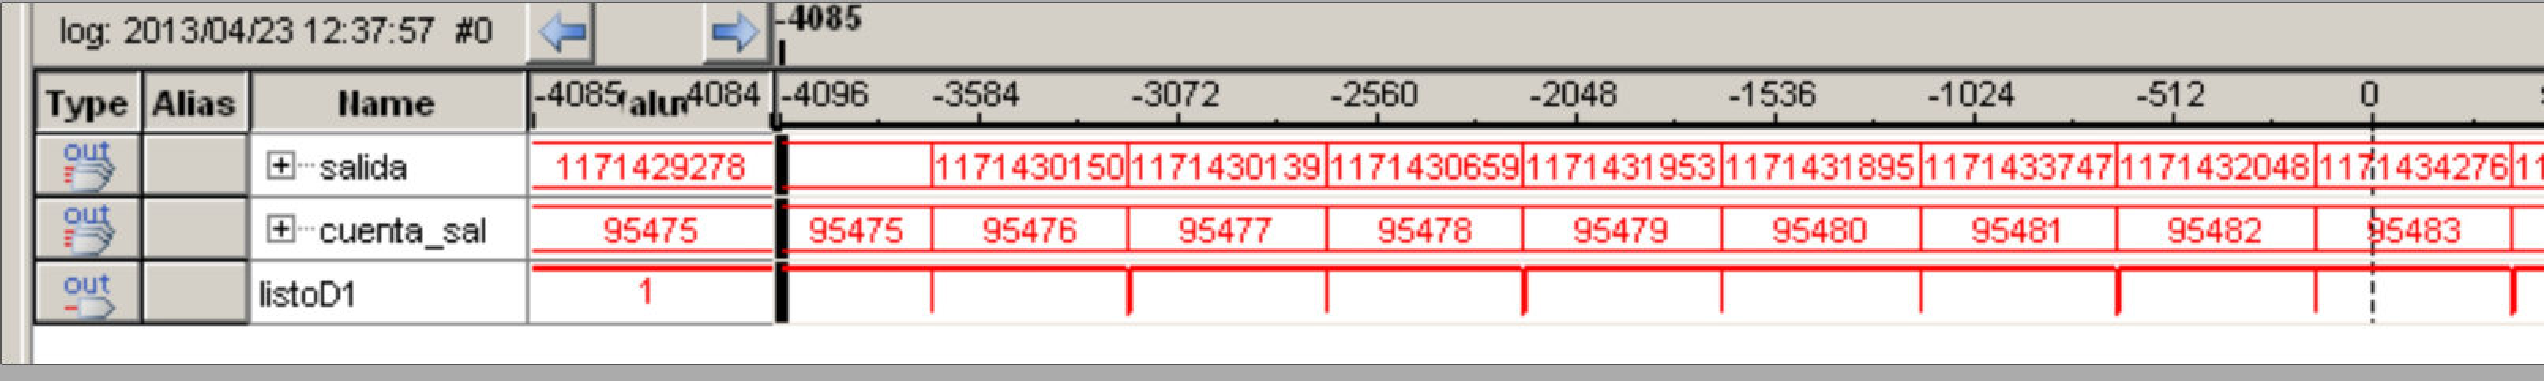
\includegraphics[width=1\columnwidth]{st.pdf}\\
	\caption{Salida del Signal Tap.}\label{fig:st}
\end{figure*}
%
\begin{figure}
	\centering
	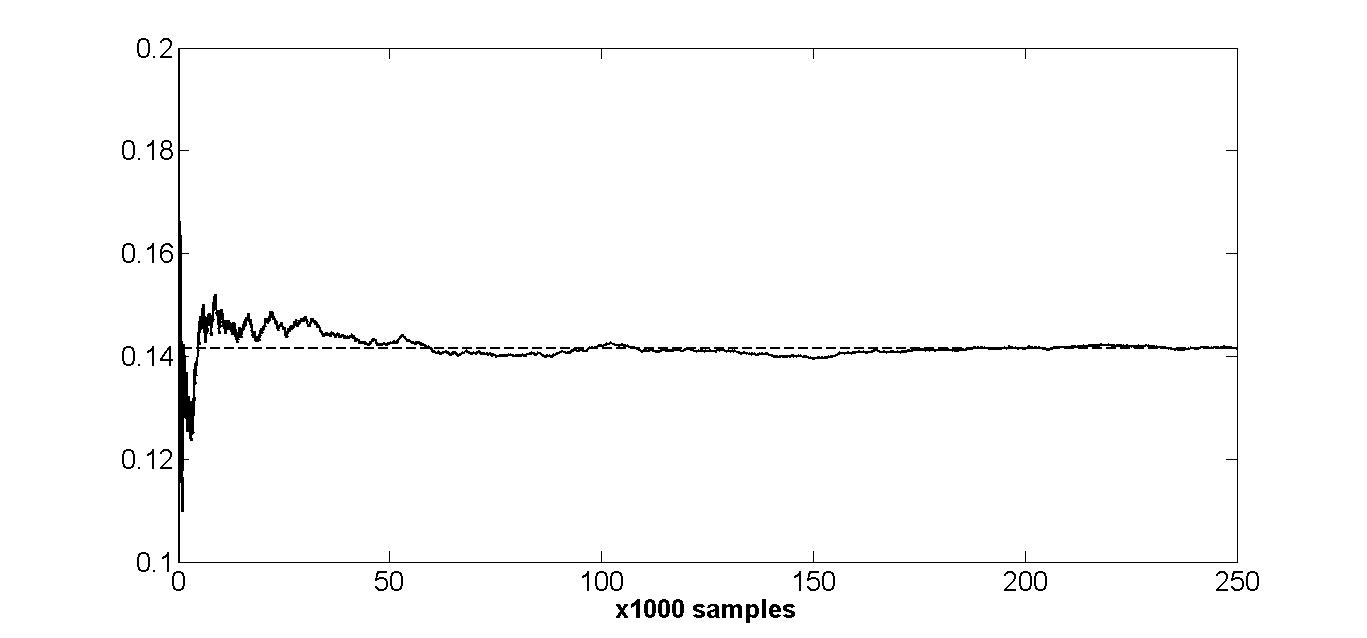
\includegraphics[width=1\columnwidth]{Lyap_MATLAB.jpg}\\
	\caption{Convergencia del algoritmo que calcula el MLE.}\label{fig:lyapu}
\end{figure}


\subsubsection{Estado actual del avance}

Actualmente estamos en etapa de desarrollo de la implementación en hardware de este algoritmo.
En este segundo caso, el sistema bajo prueba es la familia de mapas cuadráticos bidimensionales descriptos en el capítulo \ref{sec:QMaps}.

La población inicial es de $12$ coeficientes iniciales del mapa caótico empleado.
En la figura \ref{bloques} puede verse un diagrama en bloques general del sistema.
Este consiste en dos bloques principales conectados al sistema caótico bajo prueba a través de una interface wishbone.
Esto independiza el sistema del cuantificador y permite cambiar fácilmente el sistema bajo prueba.
%
\begin{figure}
	\centering
	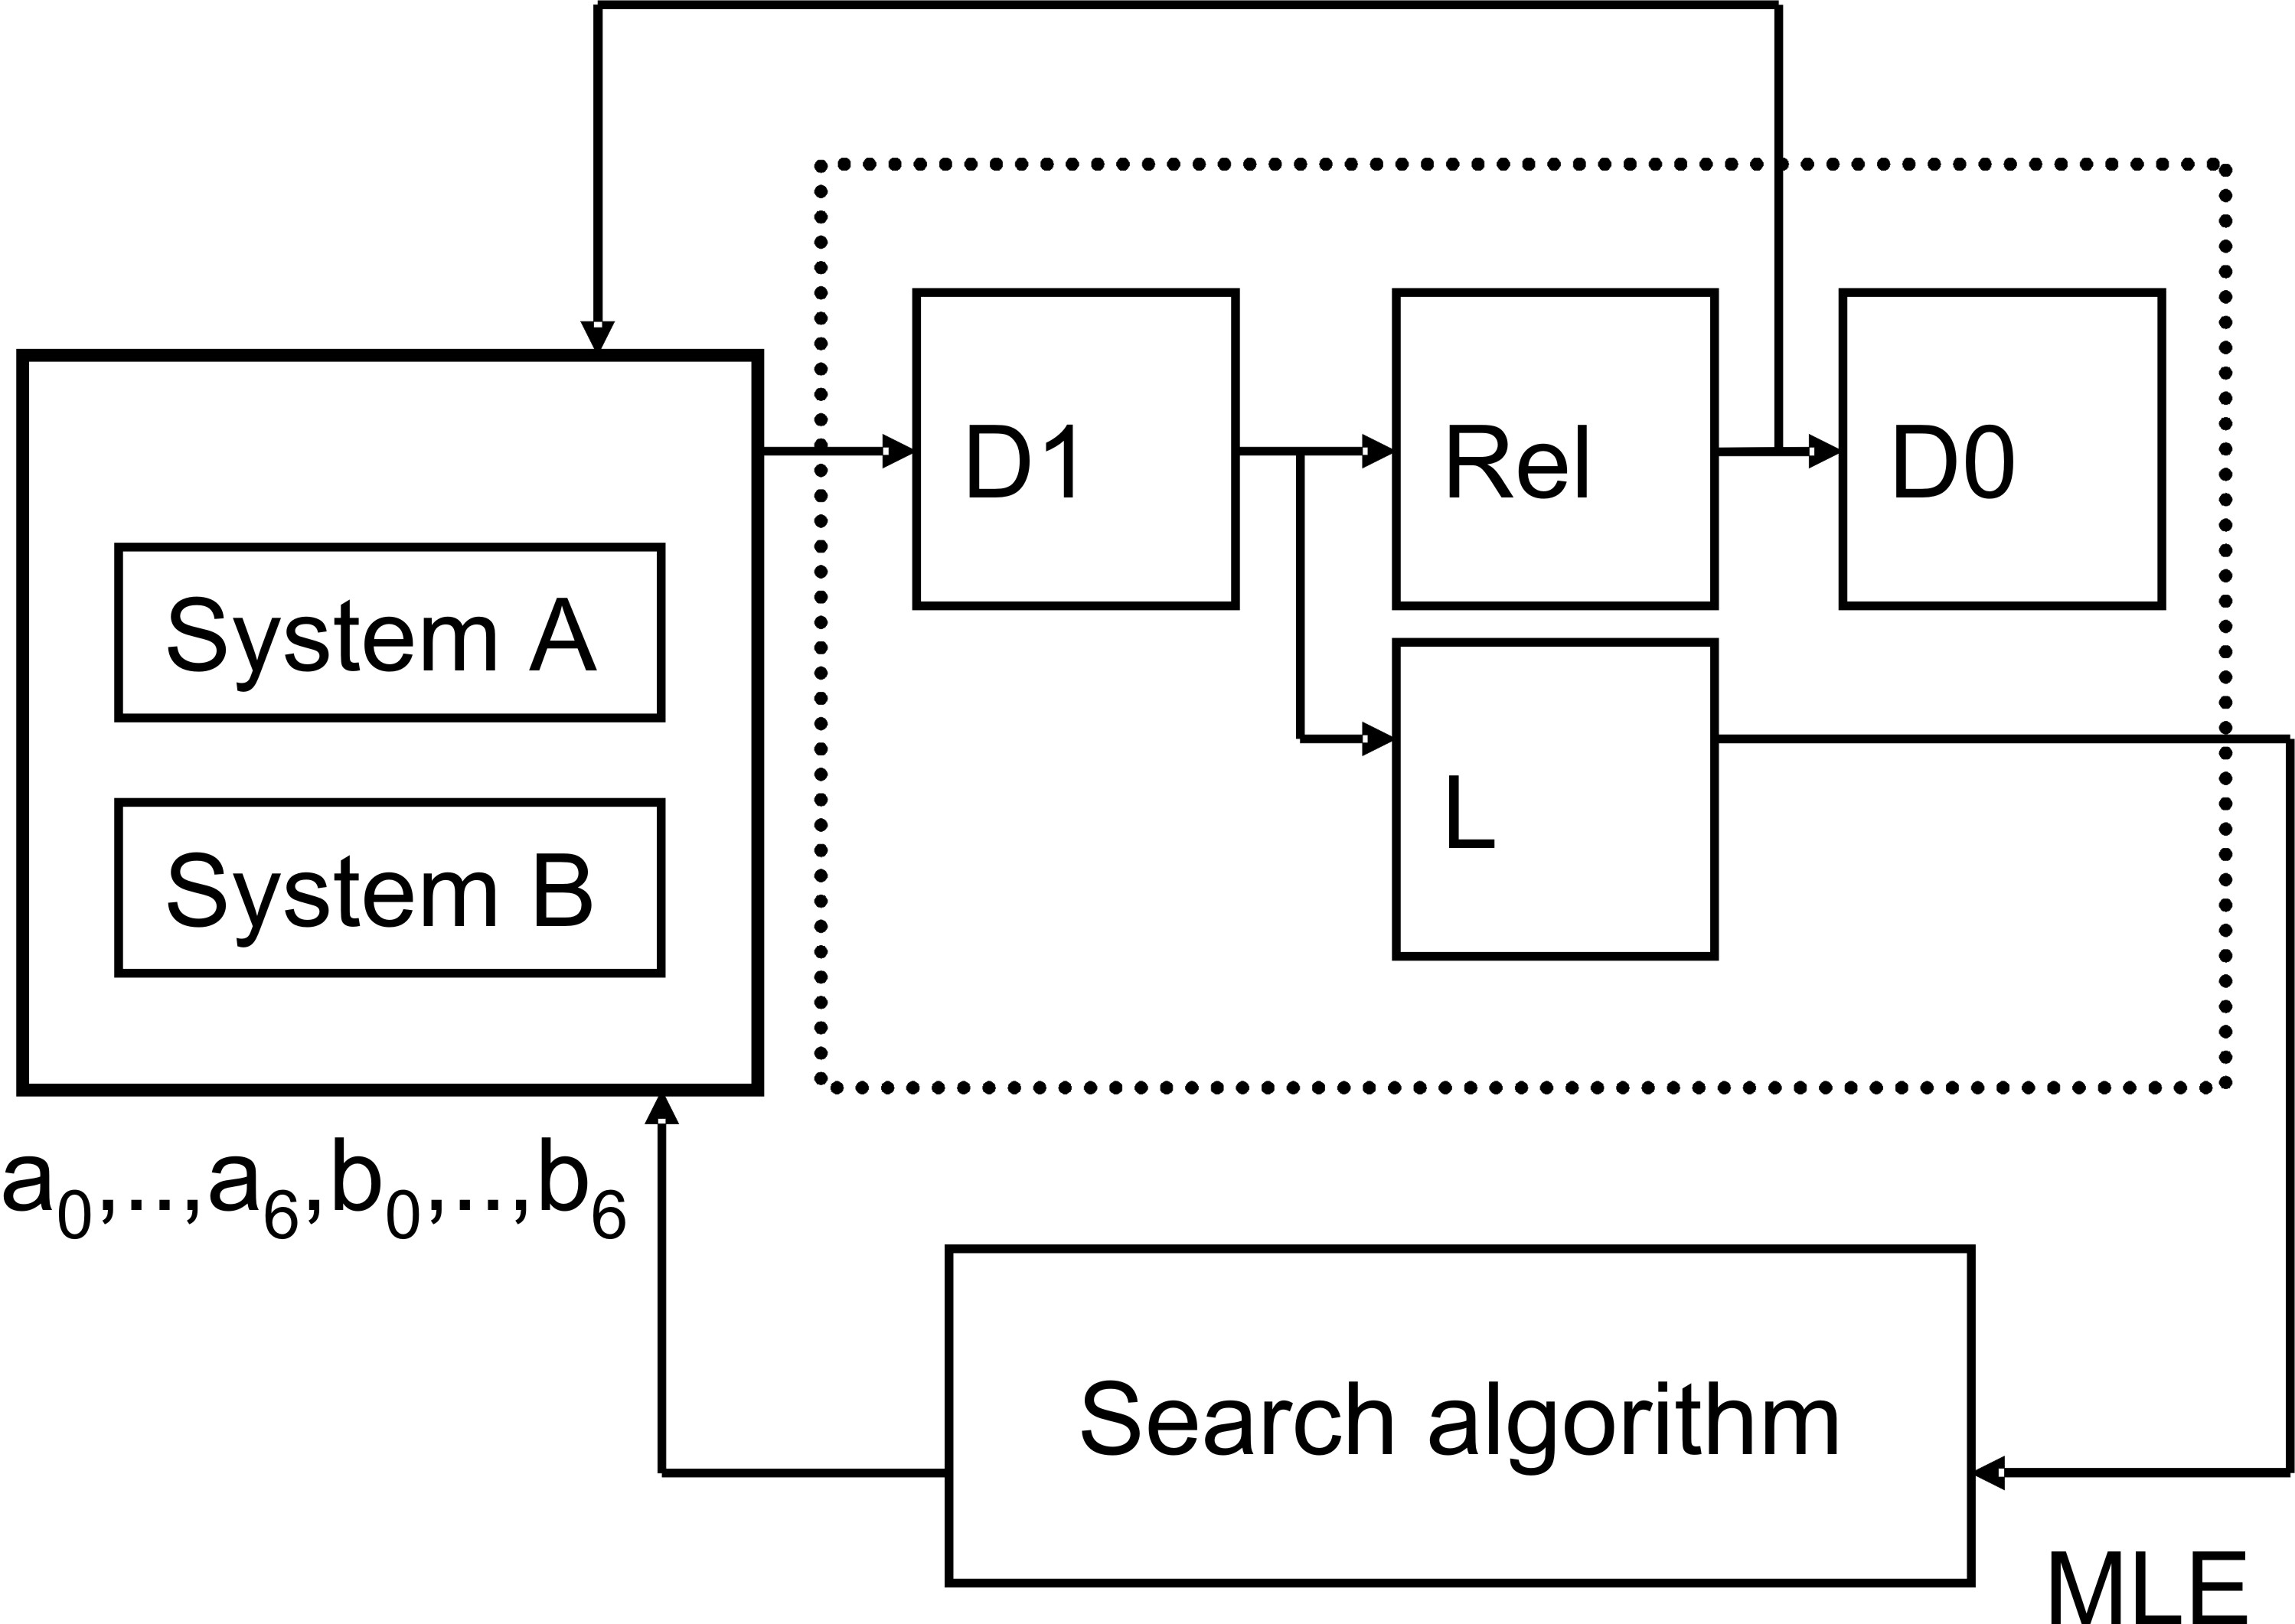
\includegraphics[width=0.85\columnwidth]{bloques.jpg}\\
	\caption{Diagrama en bloques del sistema implementado en FPGA.}\label{bloques}
\end{figure}

El sistema caótico es duplicado en dos bloques, $System A$ y $System B$.
Cada uno de ellos es inicializado con los puntos en el espacio de fases	($x_{a(i-1)}$,$y_{a(i-1)}$) y ($x_{br(i-1)}$,$y_{br(i-1)}$) respectivamente.
Cuando los sistemas caóticos terminan de calcular sus salidas, la señal digital \textit{habilita} se pone en cero y el bloque $D1$ es habilitado para calcular la distancia euclideana entre las salidas ($x_{a(i)}$,$y_{a(i)}$) y ($x_{br(i)}$,$y_{br(i)}$).

Luego se habilitan los bloques concurrentes $L$ y $Rel$.
Los puntos relocalizados que alimentan al bloque $System B$ son calculados por el bloque $Rel$.
Este bloque solo necesita los valores actuales de $d_1$ los valores previos de $d_0$, como se muestra en la ecuación \ref{eq:reubicacion}.
Cuando los puntos relocalizados $x_{br(i)}$ y $y_{br(i)}$ están disponibles, los bloques $System A$ y $System B$ se habilitan para obtener la siguiente iteración.
También se habilita el bloque $D_0$ para calcular el valor actual de $d_{0(i)}$, que se utilizará en la siguiente iteración.

Finalmente, el bloque $L$ realiza la división entre $d_0$ y $d_1$ para luego calcular el valor absoluto y el logaritmo de esta división.
El mapa es iterado $N=250000$ veces y el resultado de la sumatoria dividido por $N$ para asegurar la convergencia del método.

Cada bloque fue implementado utilizando lenguaje VHD e IP \textit{cores} provistos por \textit{Altera} (\textit{megafunctions}) cada vez que fue posible, debido a que estos \textit{cores} están optimizados para este dispositivo.
Las operaciones de punto flotante como las sumas, multiplicaciones, valores absolutos y logaritmos fueron calculadas con dichas \textit{megafunctions}.

La figura \ref{D1} muestra la implementación del bloque $D1$ en el entorno gráfico Quartus
Los puntos de salida y entrada $a$ y $b$, son tomados luego de que la señal \textit{habilita} se pone en cero.
Entonces, las señales son procesadas de acuerdo a la ecuación \ref{eq:D0D1} para calcular la distancia euclideana $d_1$.
%
\begin{figure*}
	\centering
	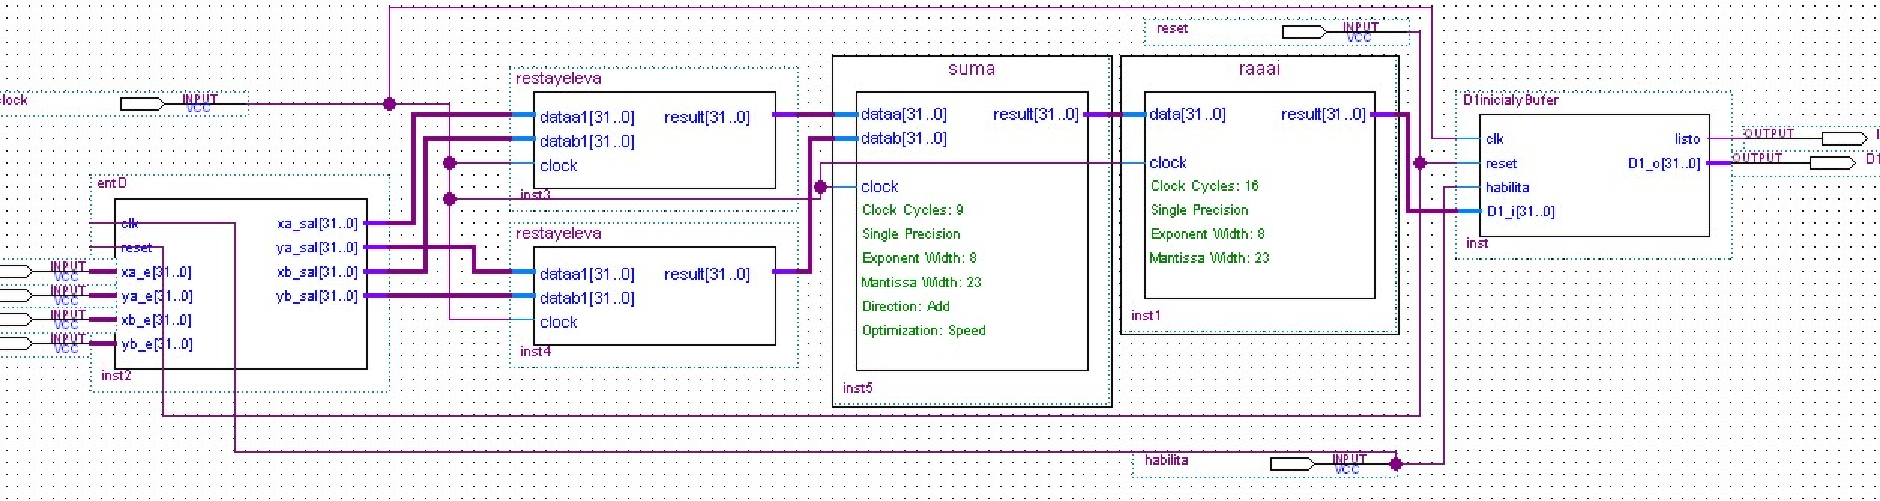
\includegraphics[width=1\columnwidth]{D1.pdf}\\
	\caption{Bloque $D_1$.}\label{D1}
\end{figure*}

La lógica del algoritmo genético fue implementada en lenguaje VHD.
Esta lógica junto con el registro de los $12$ coeficientes se muestran en la figura \ref{fig:evolutivecircuit}.
También se muesran los resultados de la compilación en la figura \ref{fig:alg_comp}.
Puede verse que esta implementación ocupa pocos recursos del dispositivo.
%
\begin{figure*}
	\centering
	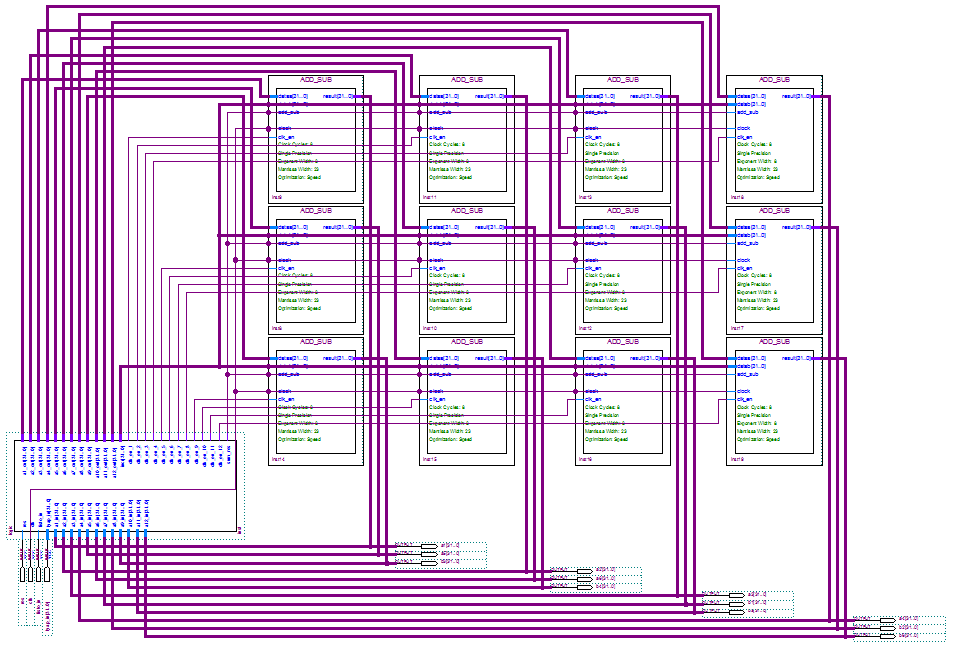
\includegraphics[width=1\columnwidth]{evolutive.png}\\
	\caption{Circuito del algoritmo evolutivo. Cada uno de los $12$ bloques ADD\_SUB guarda el valor de uno de los coeficientes $a_i$.}\label{fig:evolutivecircuit}
\end{figure*}
%
\begin{figure}
	\centering
	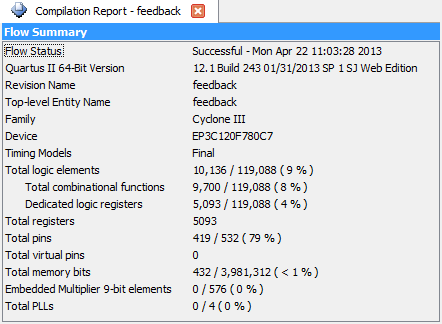
\includegraphics[width=1\columnwidth]{compilationreportalgoritmo.png}\\
	\caption{Compilation report del algoritmo evolutivo.}\label{fig:alg_comp}
\end{figure}
\section{Cuantificadores de la teoría de la información}
\label{sec:ITQs}

Dada una fuente de símbolos cuya salida es un vector de símbolos $X$, existen diferentes procedimientos para obtener una PDF \cite{Rosso2009, DeMicco2008, Mischaikow1999, Powell1979, Rosso2001, Pompe2002}.
La determinación de la mejor PDF $P$ es un problema fundamental porque $P$ y el espacio de muestra $X$ están inextricablemente vinculados.
Su aplicabilidad depende de las características particulares de los datos, tales como estacionariedad, duración de la serie temporal, variación de los parámetros, nivel de contaminación de ruido, etc.

Los cuantificadores seleccionados se basan en el recuento de símbolos y en la estadística de patrones de orden.
Las métricas a utilizar pueden clasificarse de forma amplia en dos categorías: las que cuantifican el \textit{contenido de información} de los datos en comparación con los relacionados con su \textit{complejidad}.
Obsérvese que aquí nos estamos refiriendo al espacio de funciones de densidad de probabilidad, no al espacio físico.
Para clarificar y simplificar, introducimos solamente los cuantificadores de la Teoría de la Información que se definen en PDFs discretas, ya que solo estamos tratando con datos discretos (series temporales).
Sin embargo, todos los cuantificadores también tienen definiciones para el caso continuo \cite{Shannon1948}.

\subsection{Entropía de Shannon y Complejidad Estadística}

La entropía es una cantidad básica que puede considerarse como una medida de la incertidumbre asociada (información) al proceso físico descrito por $P$.
Al tratar con el contenido de la información, la entropía de Shannon se considera a menudo como la fundamental y más natural \cite{Shannon1948}.
Considerada como una medida de la incertidumbre, es el ejemplo más paradigmático de estos cuantificadores de información.

Sea $P=\{p_i; i=1,\ldots, N\}$ con $\sum_{i=1}^N p_i = 1$, una distribución de probabilidad discreta, con $N$ el número de estados posibles del sistema bajo estudi.
La medida de la información logarítmica de shannon se denota como
\begin{equation}
\label{Shannon-disc}
S[P] ~=~ -\sum_{i=1}^{N} p_i \ln \left[ p_i \right] \ .
\end{equation}

Si $S[P] = S_{\min} = 0$, estaremos en posición de predecir con total certeza cuáles de los posibles resultados $i$, cuyas probabilidades están dadas por $p_i$, tendrán lugar realmente.
Nuestro conocimiento del proceso subyacente descrito por la distribución de probabilidad es máximo en este caso.
Por el contrario, nuestro conocimiento es mínimo para una distribución uniforme $P_e = \{p_i = 1/N; i = 1, \ldots, N \}$ dado que cada resultado exhibe la misma probabilidad de ocurrencia, y la incertidumbre es máxima, es decir, $S[P_e] = S_{\ max} = \ln N$.
Estas dos situaciones son casos extremos, por lo tanto nos centramos en la entropía de Shannon "normalizada", $0 \leq H \leq 1$, dada como
\begin{equation}
\label{shannon-disc-normalizada}
H[P] = S[P] / S_{\max} \ .
\end{equation}

Contrariamente al contenido de la información, no existe una definición universalmente aceptada de complejidad.
Aquí, nos centramos en describir la \textit{complejidad de las series temporales} y no nos referimos a la complejidad de los \textit{sistemas} subyacentes.
Un sistema complejo no genera necesariamente una salida compleja.
De hecho, los modelos "simples" pueden generar datos complejos, mientras que los sistemas "complicados" pueden producir datos de salida de baja complejidad \cite{Kantz1998}.

Una noción intuitiva de una complejidad cuantitativa atribuye valores bajos tanto a datos perfectamente ordenados (es decir, con entropía de Shannon que se va desapareciendo) como a datos aleatorios no correlacionados (con entropía Shannon máxima).
Por ejemplo, la complejidad estadística de una simple oscilación o tendencia (ordenada), pero también de ruido blanco no correlacionado (no ordenado) sería clasificada como baja.
Entre los dos casos de mínima y máxima entropía, los datos son más difíciles de caracterizar y por lo tanto la complejidad debe ser mayor.
Buscamos alguna función $C[P]$ que cuantifique las estructuras presentes en los datos que se alejan de estos dos casos.
Estas estructuras se relacionan con la organización, la estructura correlacional, la memoria, la regularidad, la simetría, los patrones y otras propiedades \cite{Feldman2008}.

Asumimos que el grado de estructuras correlacionales sería capturado adecuadamente por algún funcional $C[P]$ de la misma manera que la entropía de Shannon $S[P]$ \cite{Shannon1948} ``capta " la aleatoriedad.
Claramente, las estructuras ordinales presentes en un proceso no son cuantificadas por medidas de aleatoriedad y, por consiguiente, son necesarias medidas de complejidad estadística o estructural para una mejor comprensión (caracterización) de la dinámica del sistema representada por sus series temporales \cite{Feldman1998}.

Una medida adecuada de complejidad puede definirse como el producto de una medida de información y una medida de desequilibrio, es decir, algún tipo de distancia de la distribución equiprobable de los estados accesibles de un sistema.
En este sentido, en \cite{Lamberti2004} los autores introdujeron una eficaz {\it Medida de Complejidad Estadística \/} (SCM) $C$, que es capaz de detectar detalles esenciales de los procesos dinámicos subyacentes al conjunto de datos.
Basado en el trabajo de López-Ruiz \cite{Lopez1995}, esta medida de complejidad estadística \cite{Martin2003,Lamberti2004} se define a través de la forma del producto
\begin{equation}
C[P] = Q_{J}[P,P_e] \cdot H[P]
\label{complexity}
\end{equation}
de la entropía de Shannon normalizada $H$, ver eq. \eqref{shannon-disc-normalizada}, y el desequilibrio $Q_{J}$ definido en términosde la divergencia de Jensen-Shannon $J[P, P_e]$.
Esto es,
\begin{equation}
\label{disequilibrium}	
Q_{J} [ P, P_e] = Q_{0} J[ P, P_e] = Q_{0} \{ S[(P + P_e)/2 ] - S[ P ]/2 - S[P_e]/2\},
\end{equation}
en la divergencia de Jensen-Shannon mencionada arriba, $Q_0$ es una constante de normalización tal que $0 \leq Q_{J} \leq 1$:
\begin{equation}
Q_0 ~=~ -2 \left\{ {\frac{N+1}{N}} \ln (N+1) - \ln (2N) + \ln N \right\}^{-1} \ ,
\label{q0-jensen-1}
\end{equation}
y es igual a la inversa del máximo valor posible de $J [P,P_e]$.
Este valor es obtenido cuando una de las componentes de $P$, digamos $p_m$, es igual a uno y todos los $p_j$ restantes son cero.

La divergencia de Jensen-Shannon, que cuantifica la diferencia entre las distribuciones de probabilidad, es especialmente útil para comparar la composición simbólica entre diferentes secuencias \cite{Grosse2002}.
Obsérvese que la SCM introducida anteriormente depende de dos distribuciones de probabilidad diferentes: una asociada con el sistema analizado, $P$, y la otra con la distribución uniforme, $P_e$.
Además, se demostró que para un valor dado de $H$, el rango de valores posibles de $C$ varía entre un mínimo $C_ {min}$ y un máximo $C_ {max}$, restringiendo los posibles valores del SCM \cite{Martin2006}.

Por lo tanto, está claro que información adicional importante relacionada con la estructura correlacional entre los componentes del sistema físico se proporciona evaluando la medida de la complejidad estadística.

\subsection{Determinación de la distribución de probabilidad}

La evaluación de los cuantificadores derivados de la Teoría de la Información supone algún conocimiento previo sobre el sistema; específicamente para aquellos introducidos previamente (entropía de Shannon y complejidad estadística), una distribución de probabilidad asociada a la serie temporal en análisis debe proporcionarse antes.
La determinación del PDF más adecuado es un problema fundamental porque la PDF $P$ y el espacio de muestra $\Omega$ están intrincadamente vinculados.

Las metodologías usuales asignan a cada valor de la serie $X(t)$ (o conjunto de valores consecutivos no superpuestos) un símbolo de un alfabeto finito $A = \{a_1, \dots, a_M \}$, creando así una {\it secuencia simbólica \/} que puede considerarse como una descripción de la serie cronológica en cuestión.
Como consecuencia, las relaciones de orden y las escalas temporales de la dinámica se pierden por completo.

Es importante resltar que $P$ en si, no es un objeto con una definición única y existen varias aproximaciones para ``asociar'' una dada $P$ con una dada serie de tiempo.
Solo para mencionar algunos criterios de extracción utilizados frecuentemente en la literatura: {\it a)\/} histogramas de series temporales \cite{Martin2004}, {\it b)\/} dinámica simbólica binaria \cite{Mischaikow1999}, {\it c)\/} análisis de Fourier \cite{Powell1979}, {\it d)\/} trensformadas wavelet \cite{Blanco1998,Rosso2001}, {\it e)\/} PDF de particiones \cite{Ebeling2001}, {\it f)\/} PDF de permutaciones \cite{Pompe2002,Keller2005}, {\it g)\/} PDF discreta \cite{Amigo2007}, etc.
Hay una amplia libertad para elegir entre ellas y la aplicación específica debe ser analizada para hacer una buena elección.

Se puede incorporar debidamente la información causal si se incluye información sobre la dinámica pasada del sistema en la secuencia simbólica, es decir, los símbolos del alfabeto $A$ se asignan a una porción del espacio de fase o trayectoria.
Bandt y Pompe (BP) \cite{Bandt2002} introdujeron una metodología simbólica simple y robusta que toma en cuenta el ordenamiento temporal de las series temporales comparando valores vecinos en una serie temporal.
La propiedad de causalidad de la PDF permite que los cuantificadores (basados en esta PDF) discriminan entre sistemas determinísticos y estocásticos \cite{Rosso2007B}.
Los datos simbólicos son:
{\it (i) \/} ~ creados por la clasificación de los valores de la serie; y
{\it (ii) \/} ~ definidos por el reordenaminto de los datos embebidos en orden ascendente, lo que equivale a una reconstrucción de espacio de fase con dimensión de emmbedding (longitud de patrón) $D$ y retardo de tiempo $\tau$.
De esta forma, es posible cuantificar la diversidad de los símbolos de ordenación (patrones) derivados de una serie temporal escalar.
Obsérvese que la secuencia de símbolos apropiada surge naturalmente de la serie temporal, y no se necesitan suposiciones basadas en modelos.
El procedimiento es el siguiente:
\begin{itemize}
	\item Dada una serie $\{x_t; t=0, \Delta t, \cdots,N\Delta t \}$, se genera una secuencia de vectores de longitud $D$.
	\begin{equation}
	(s)\longmapsto\left(x_{t-(d-1)\Delta t},x_{t-(d-2)\Delta t},\dots,x_{t-\Delta t},x_{t}\right) 
	\label{eq:vectores}
	\end{equation}
	Cada vector resulta ser la "historia" del valor $x_t$. Evidentemente, cuanto más larga sea la longitud de los vectores $D$, mayor será la información sobre la historia de los vectores, pero se requiere un valor más alto de $N$ para tener una estadística adecuada.
	\item Las permutaciones $\pi=(r_0, r_1, \cdots, r_{D-1})$ de $(0, 1, \cdots, D-1)$ es llamado ``patrón de orden'' de tiempo $t$, definido por:
	\begin{equation}
	\label{eq:permuta}
	x_{t-r_{D-1}\Delta t}\le x_{t-r_{D-2}\Delta t}\le\dots\le x_{t-r_{1}\Delta t}\le x_{t-r_0\Delta t}
	\end{equation}
	Para obtener se un resultado único se considera $r_i<r_{i-1}$ si $x_{t-r_{i}\Delta t}=x_{t-r_{i-1}\Delta t}$.
	De esta forma, todas las $D!$ permutaciones posibles $\pi$ de orden $D$, y la PDF $P=\{p(\pi)\}$ es definida como:
	\begin{equation}
	\label{eq:frequ}
	p(\pi)=\frac{\sharp \{s|s\leq N-D+1; (s) \quad \texttt{has type}~\pi\}}{N-D+1}
	\end{equation}
	En estas últimas expresiones, el símbolo $\sharp$ denota cardinalidad.
\end{itemize}

Por lo tanto, una distribución de probabilidad de patrones de órden $P = \{ p(\pi_i), i = 1, \dots, D! \}$ se obtiene de la serie temporal.
De esta manera, el vector definido por la ecuación \eqref{eq:frequ} se convierte en un símbolo único $\pi$.
Se establece $r_i < r_{i-1}$ si $x_{s-r_{i}} = x_{s-r_{i-1}}$ para la obtener una única solución.
La única condición para la aplicabilidad del método BP es una suposición estacionaria muy débil: para $k \leq D$, la probabilidad para $x_t<x_{t + k}$ no debe depender de $t$.
Con respecto a la selección de los parámetros, Bandt y Pompe sugirieron trabajar con $3 \leq D \leq 6$ para longitudes de series de tiempo típicas, y específicamente se consideró un retraso de tiempo $\tau = 1$ en su publicación principal.

Para destacar la diferencia entre una $P$ \textit{causal} y una \textit{no causal}, consideremos una serie de valores $X=\{x_i,~i=1,2,...\}$ generada por la función $randn$ de Matlab's $^\copyright$; consideremos también la serie $Y=\{y_i,~i=1,2,...\}$ como la resultante de ordenar la serie $X$ en forma ascendente. Esto se puede ver en el ejemplo en la figura \ref{fig:causal_nocausal}, en la figura \ref{subfig:causal_nocausal_x} se muestran 1000 valores sorteados con una distribución uniforme entre 0 y 1, también mostramos en la figura \ref{subfig:causal_nocausal_y} la versión ordenada de la serie de la figura \ref{subfig:causal_nocausal_x}, son los mismos valores pero ordenados en forma ascendente. Una $P$ no causal es el histograma normalizado que mostramos en las figuras \ref{subfig:causal_nocausal_HistValx} y \ref{subfig:causal_nocausal_HistValy}, en donde puede verse que $P(X)$ es idéntica a $P(Y)$, por lo que todos los cuantificadores que se calculen a partir de ellas serán idénticos para las dos series. Una $P$ causal puede ser obtenida mediante el procedimiento de Bandt \& Pompe descripto arriba, en este caso $P(X)$ de la figura \ref{subfig:causal_nocausal_HistBPx} es bastante uniforme y $P(Y)$ de la figura \ref{subfig:causal_nocausal_HistBPy} tiene una forma tipo delta. En este caso, $P$ registra que $Y$ es monótonamente creciente y presenta un solo patrón de orden.

\begin{figure}[htpb]
	\centering
	\begin{subfigure}[t]{0.49\textwidth}
		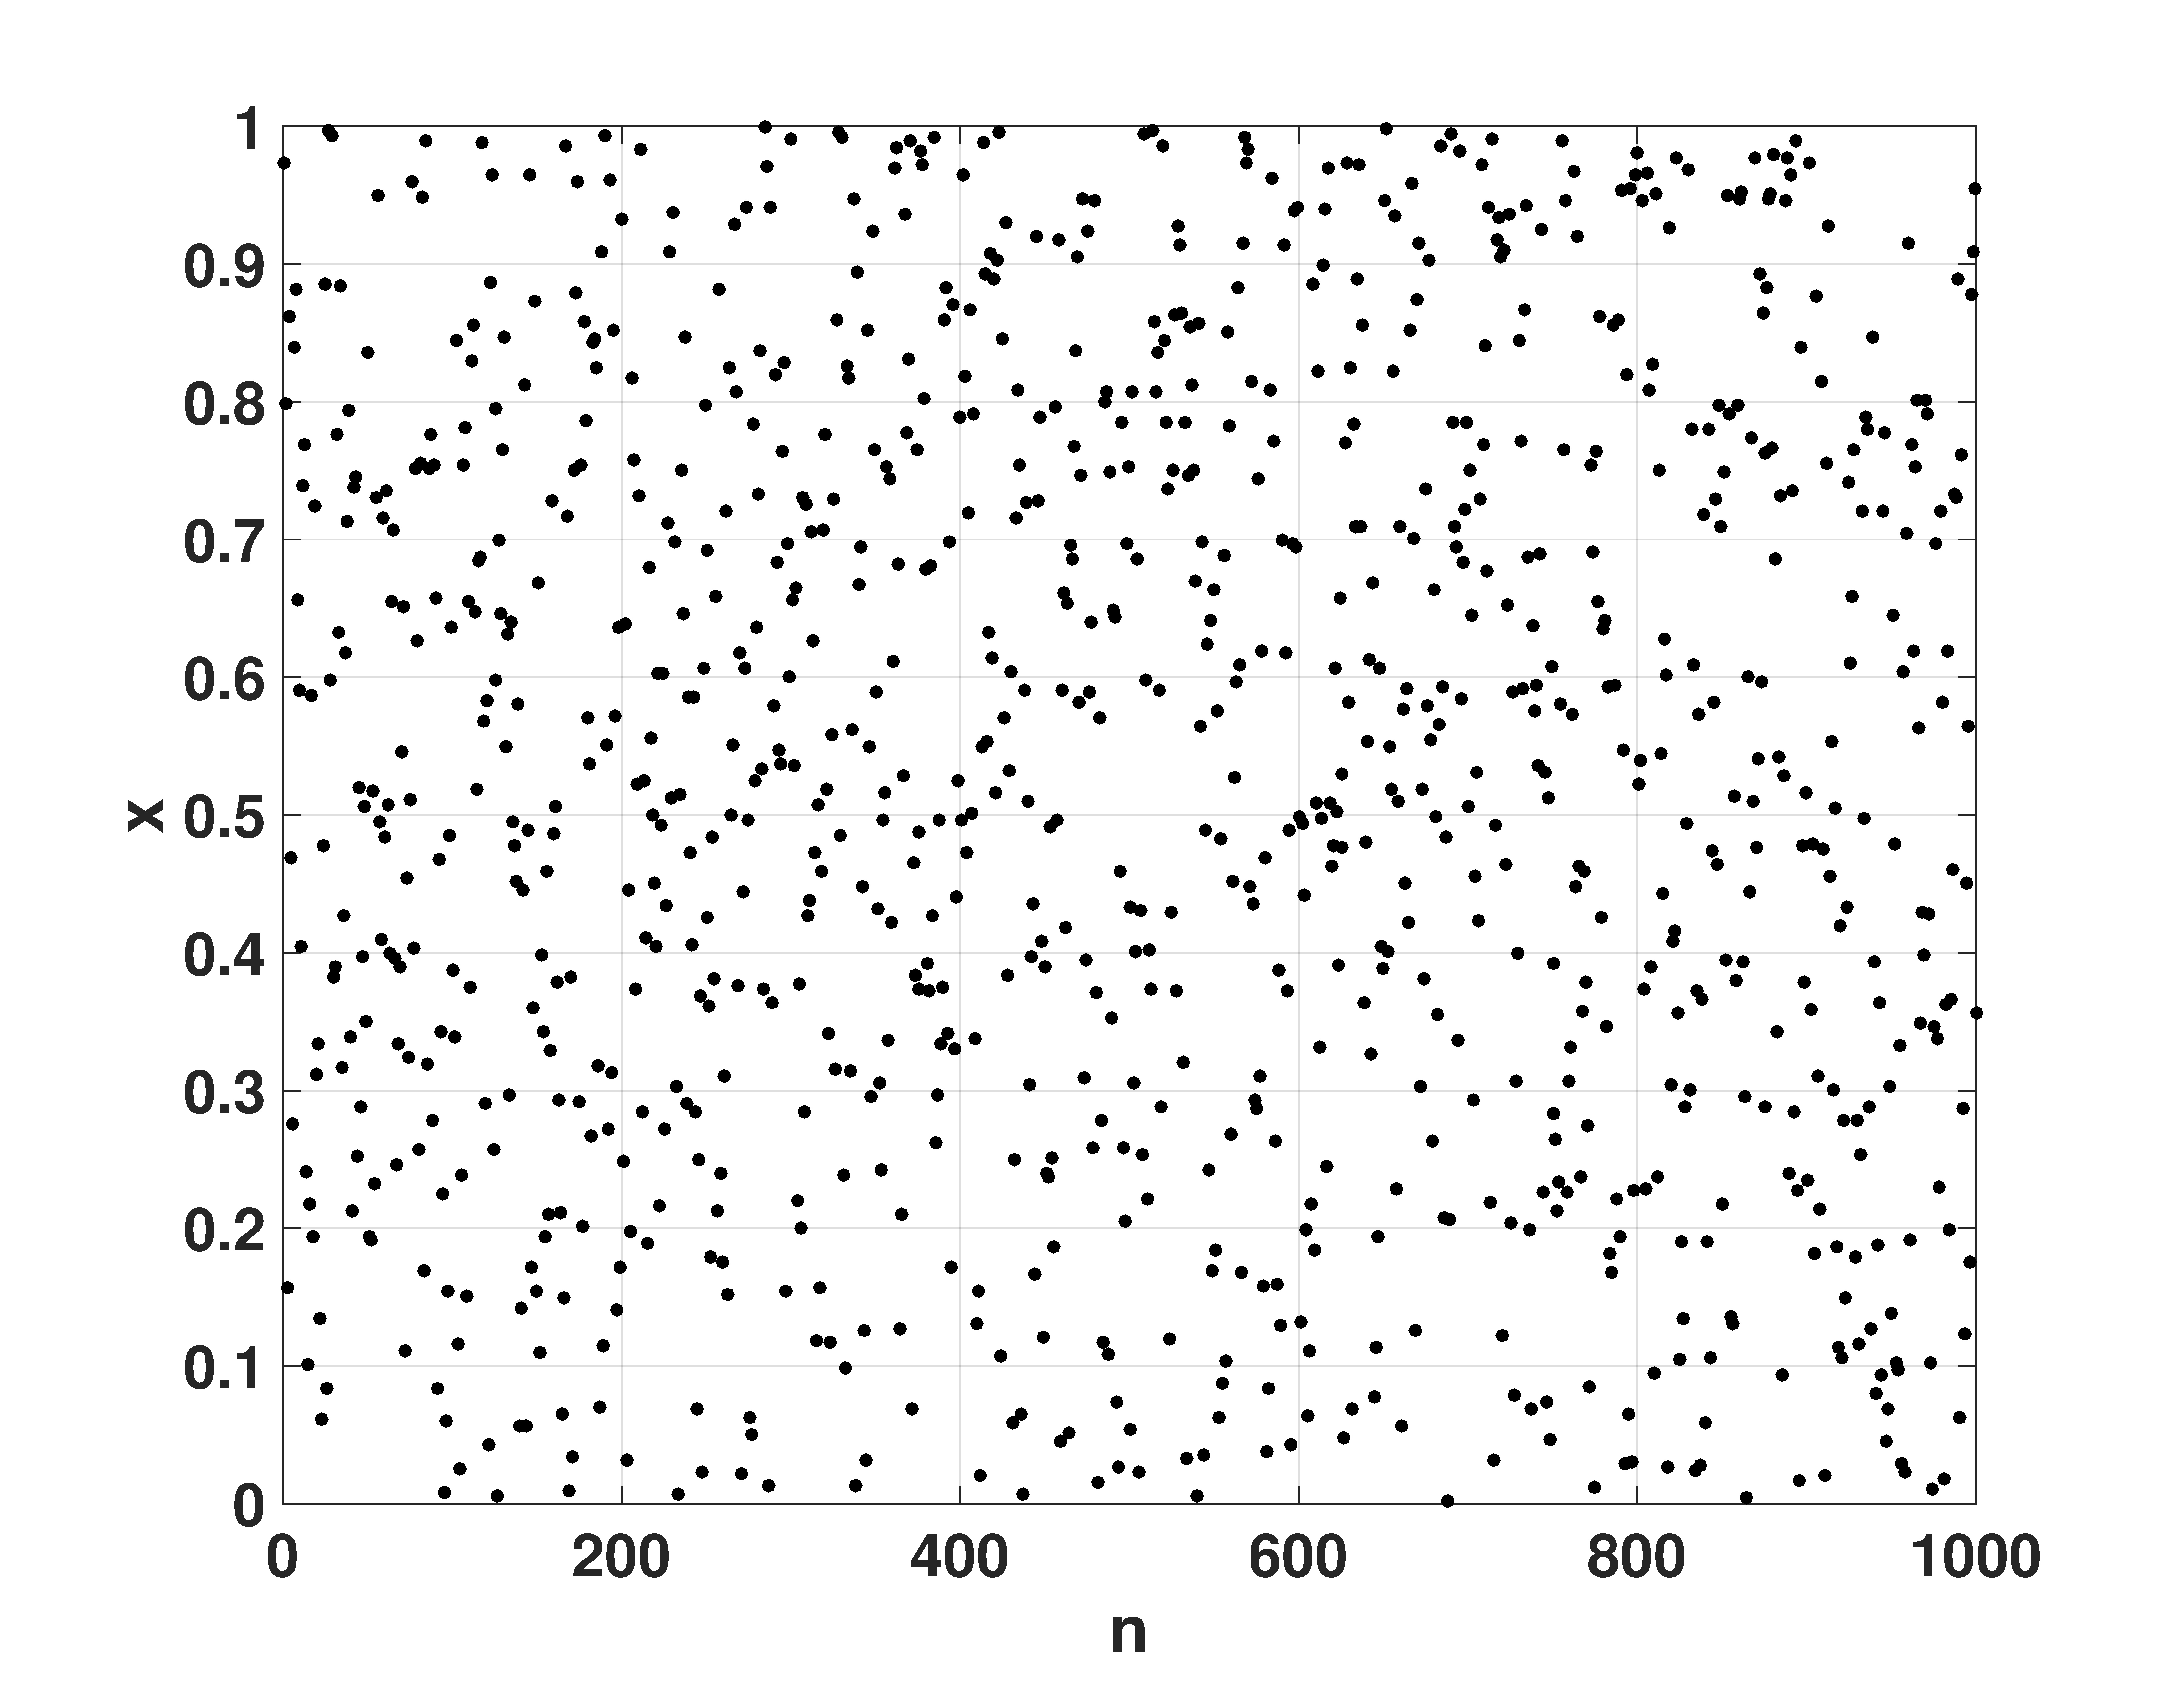
\includegraphics[width=\textwidth]{x}
		\caption{$1000$ puntos con distribución uniforme}
		\label{subfig:causal_nocausal_x}
	\end{subfigure}
	\begin{subfigure}[t]{0.49\textwidth}
		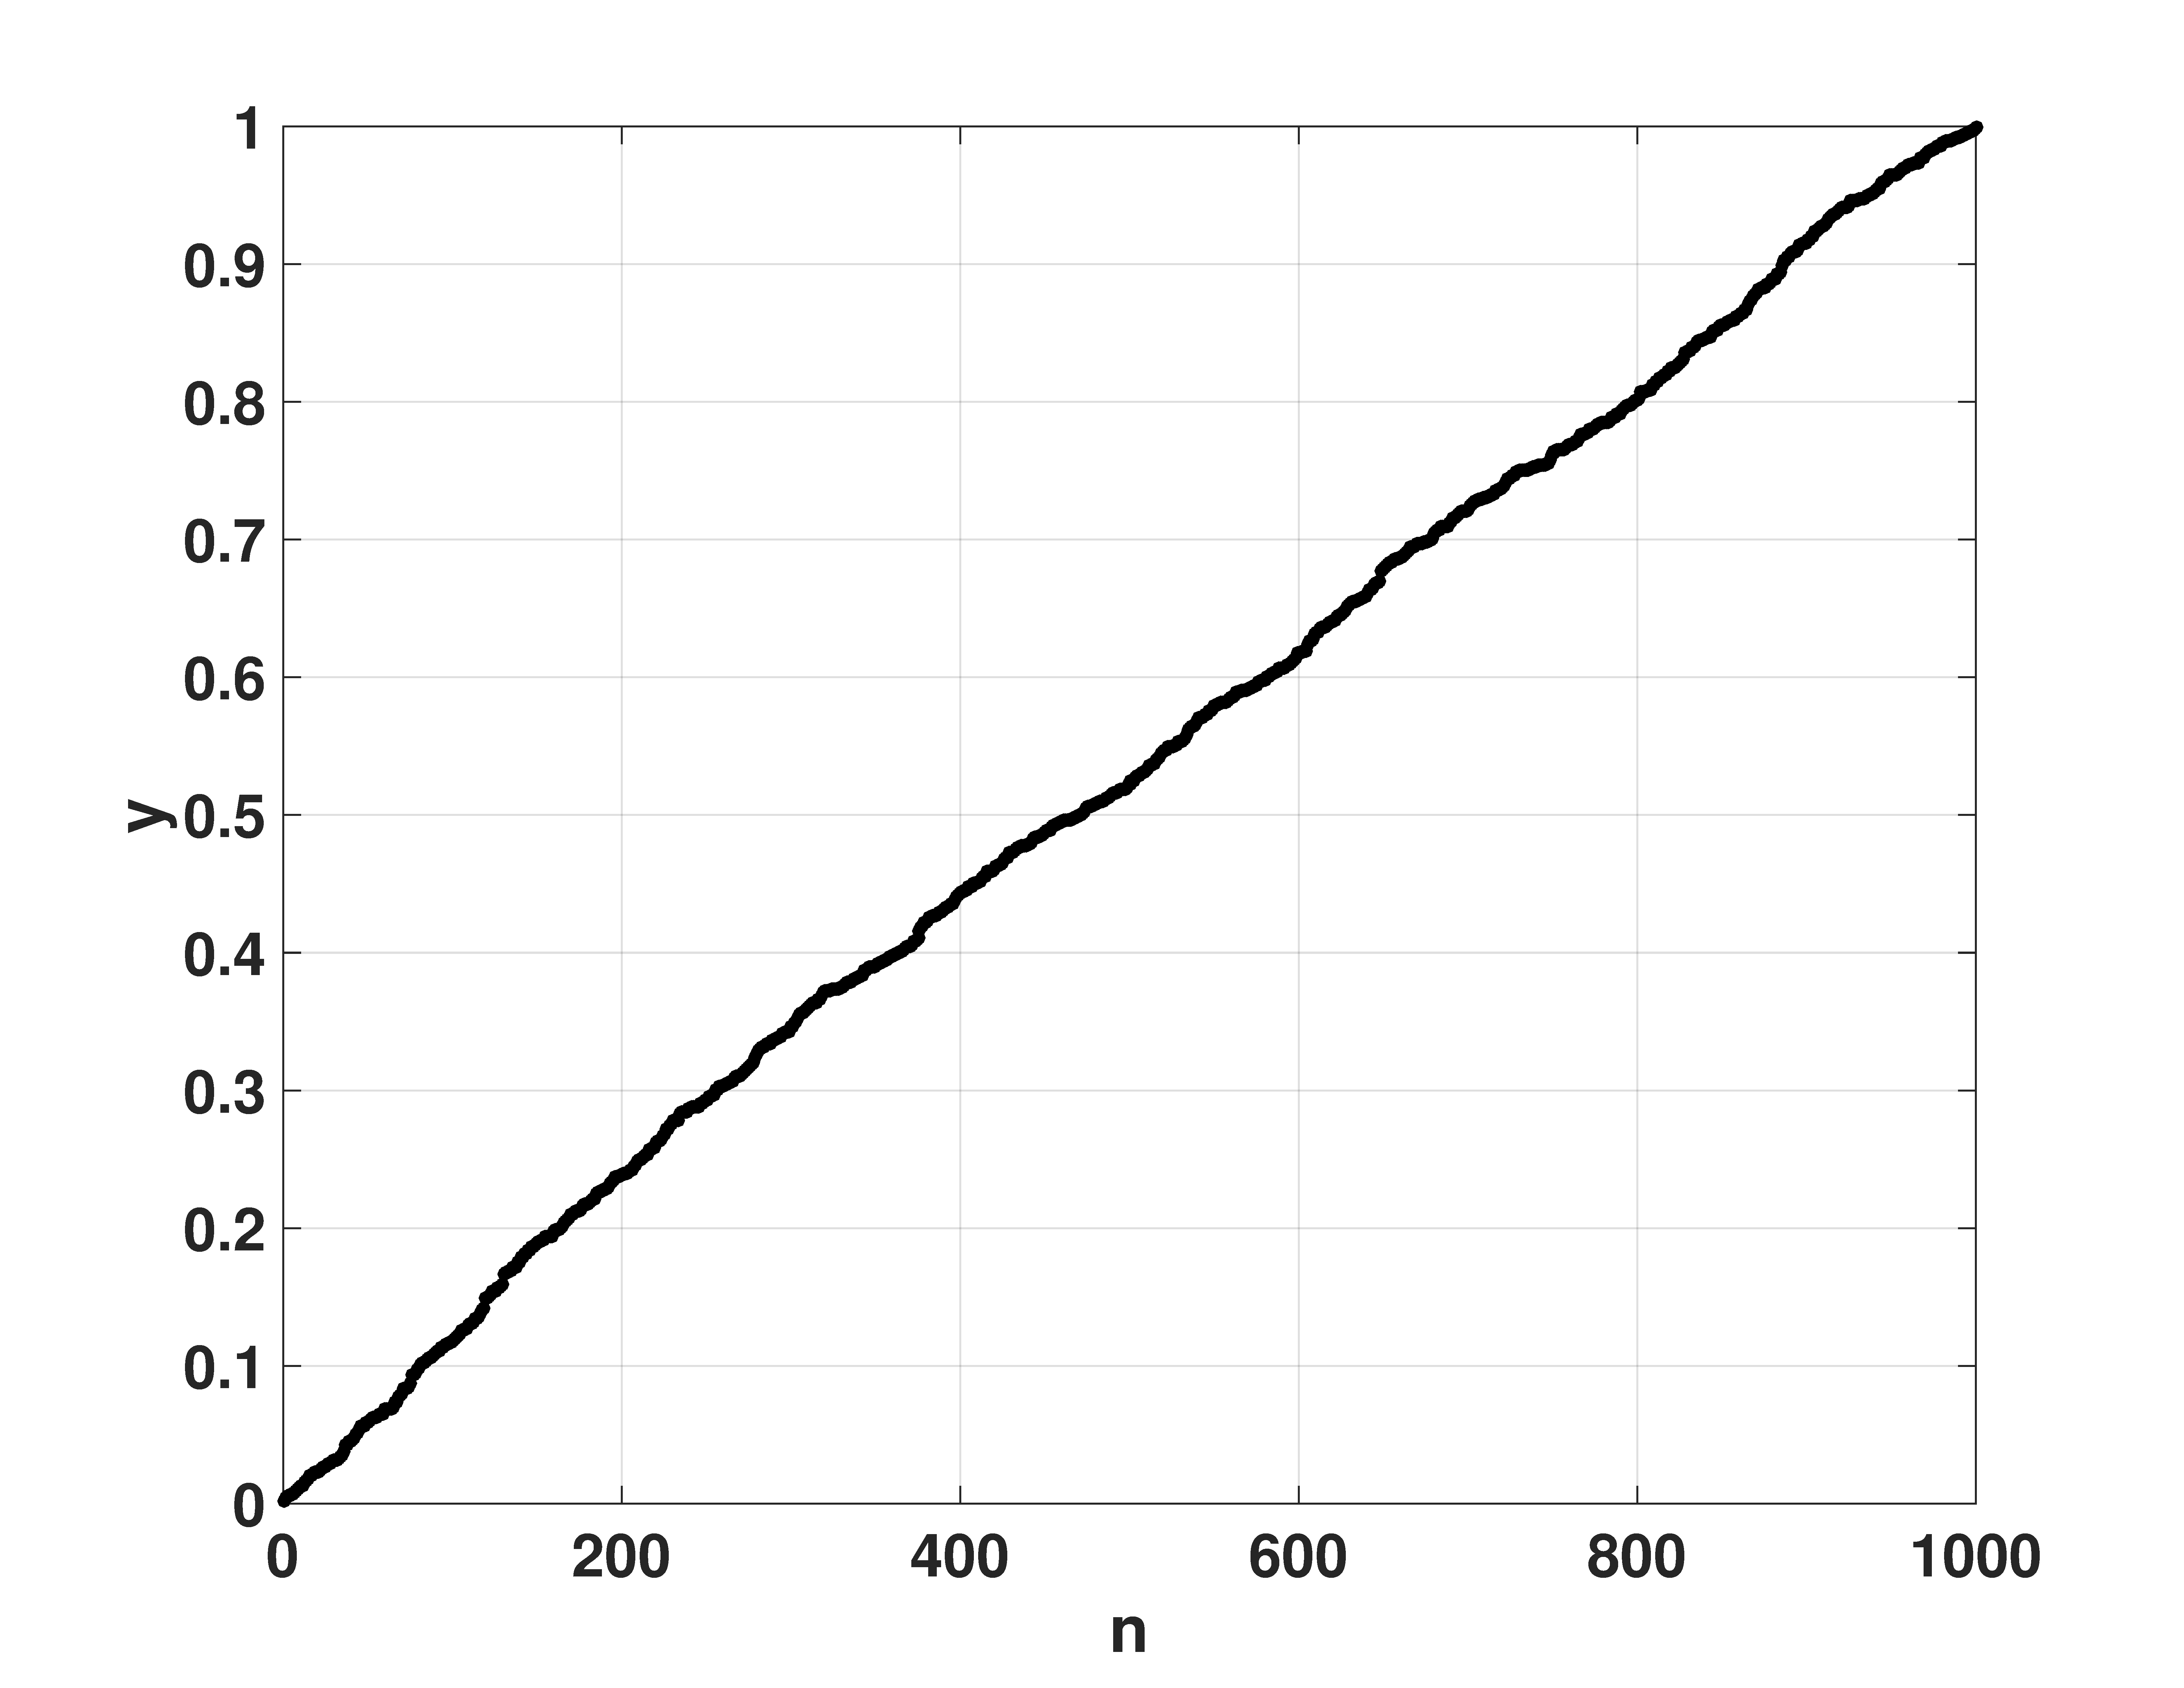
\includegraphics[width=\textwidth]{y}
		\caption{Puntos ordenados}
		\label{subfig:causal_nocausal_y}
	\end{subfigure}
	\begin{subfigure}[t]{0.49\textwidth}
		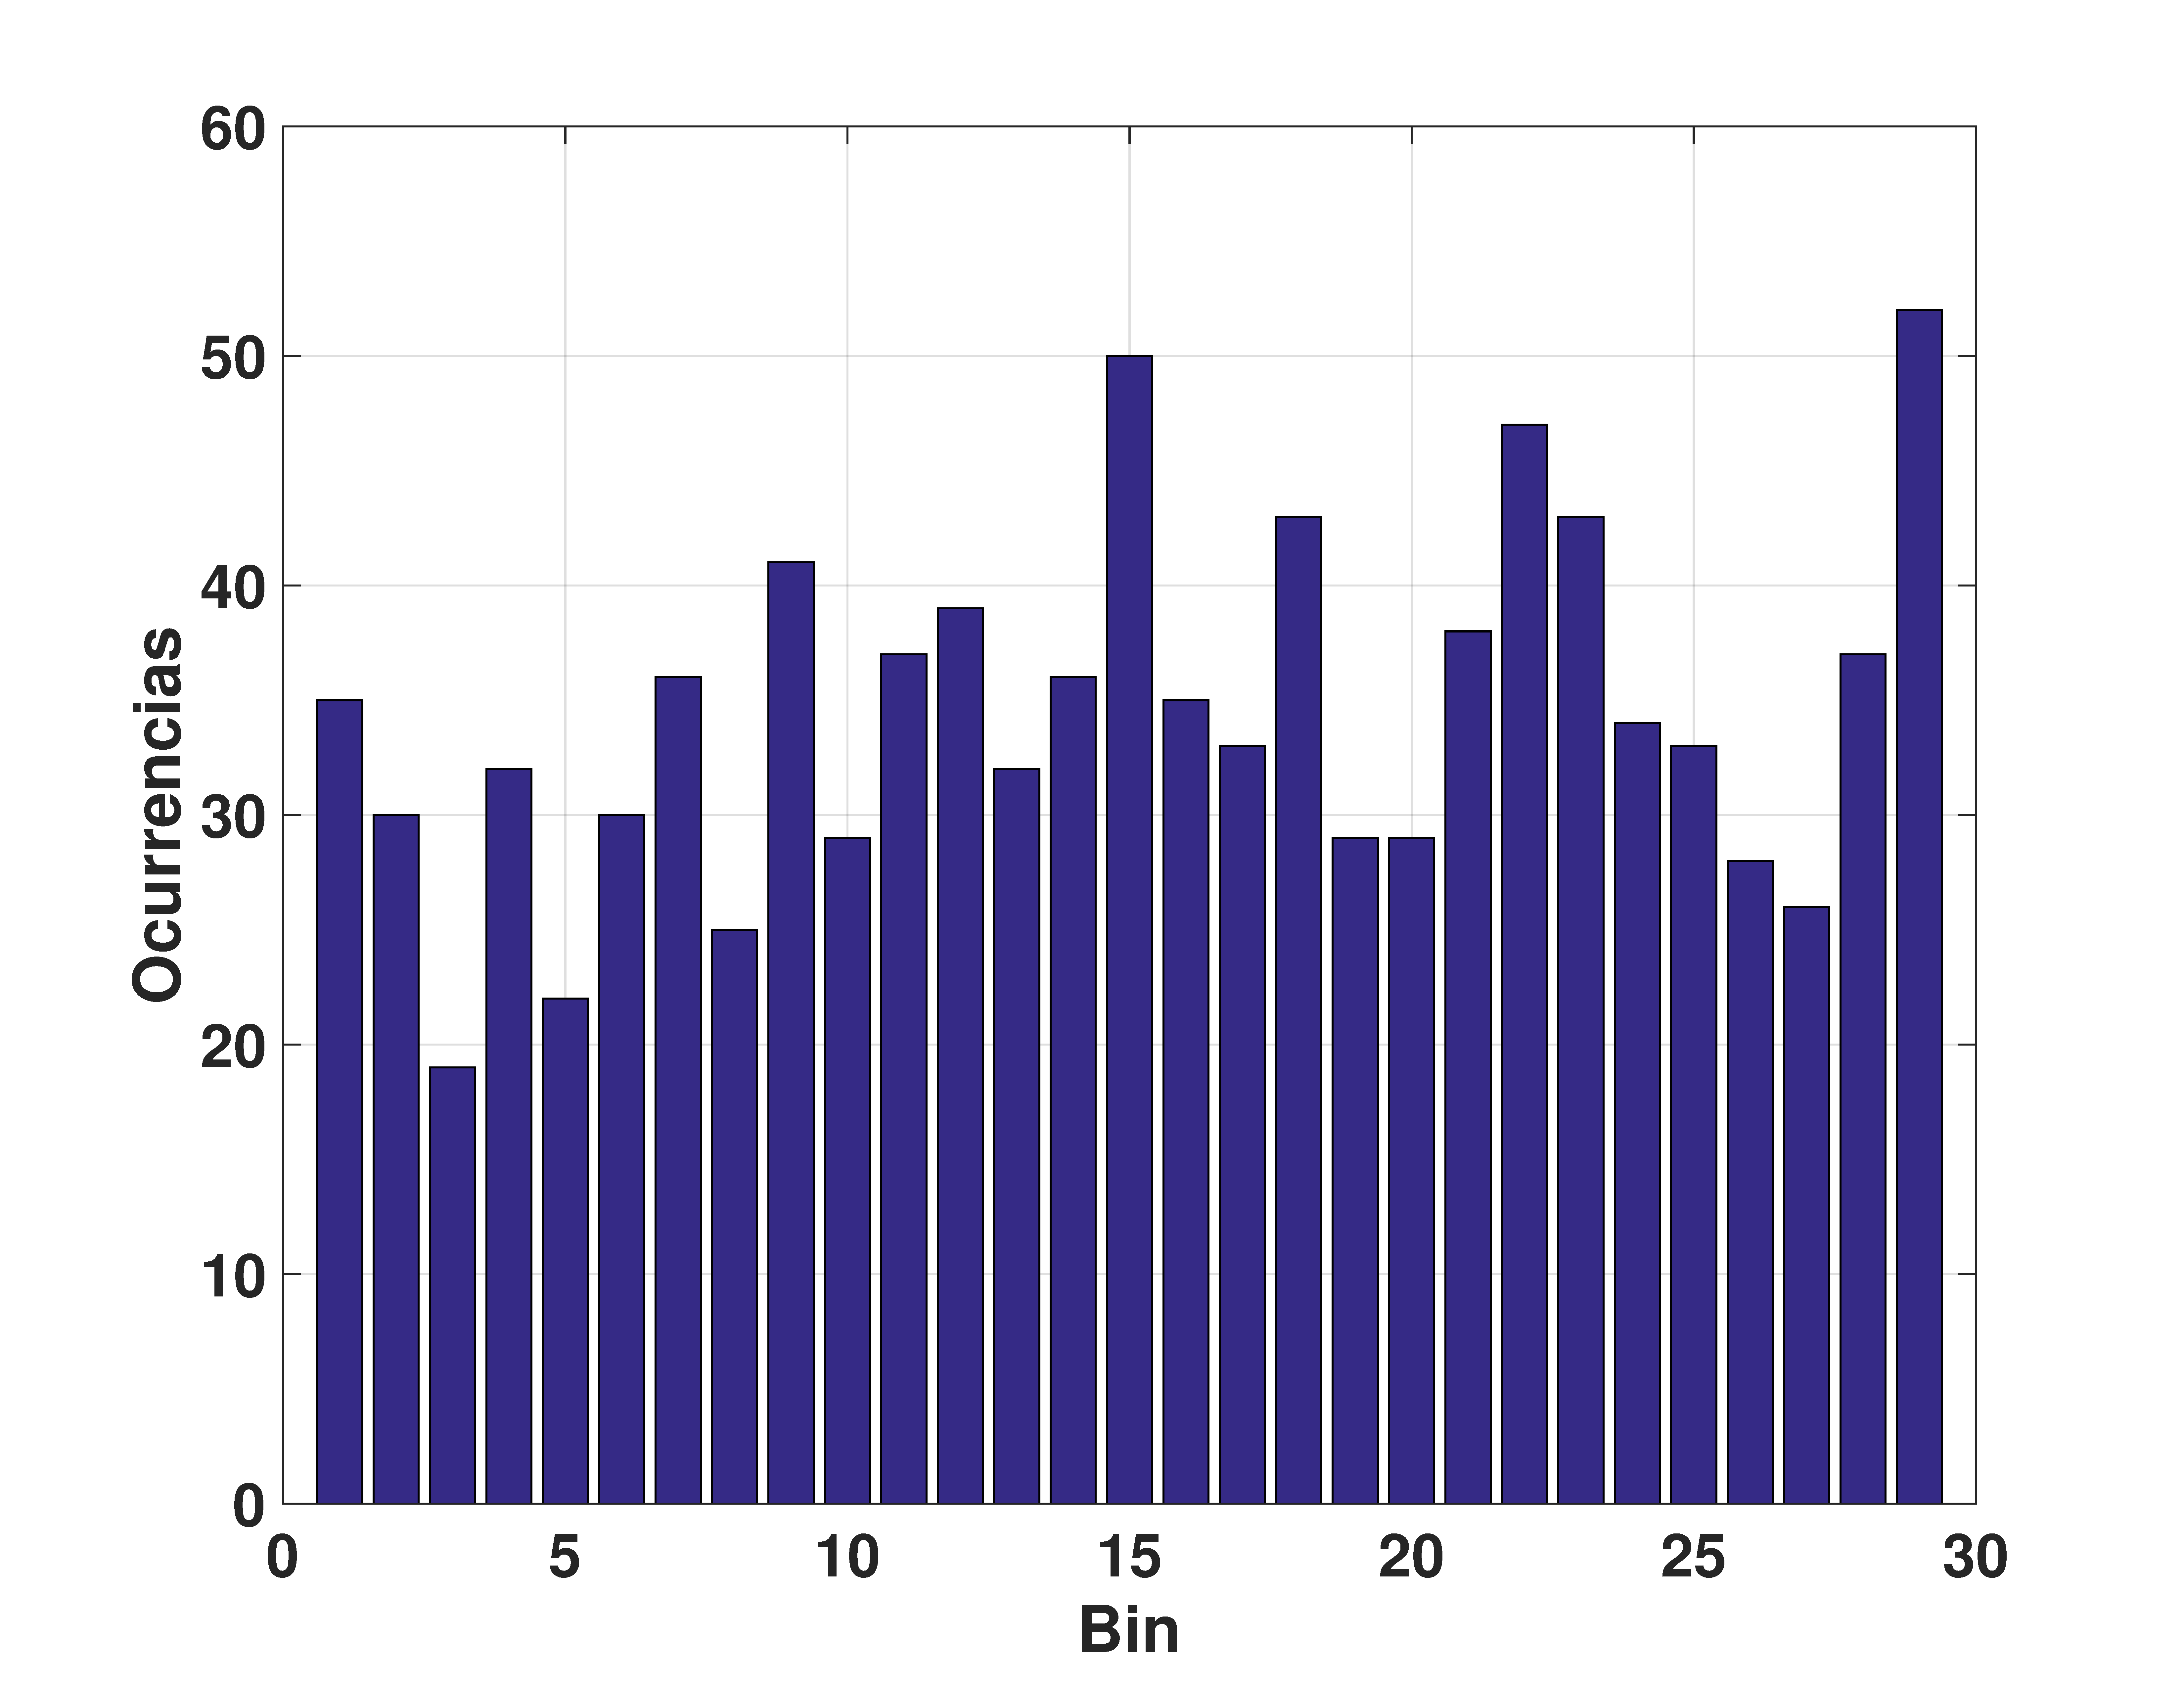
\includegraphics[width=\textwidth]{HistVal_x}
		\caption{Histograma de valores de los puntos sin ordenar}
		\label{subfig:causal_nocausal_HistValx}
	\end{subfigure}
	\begin{subfigure}[t]{0.49\textwidth}
		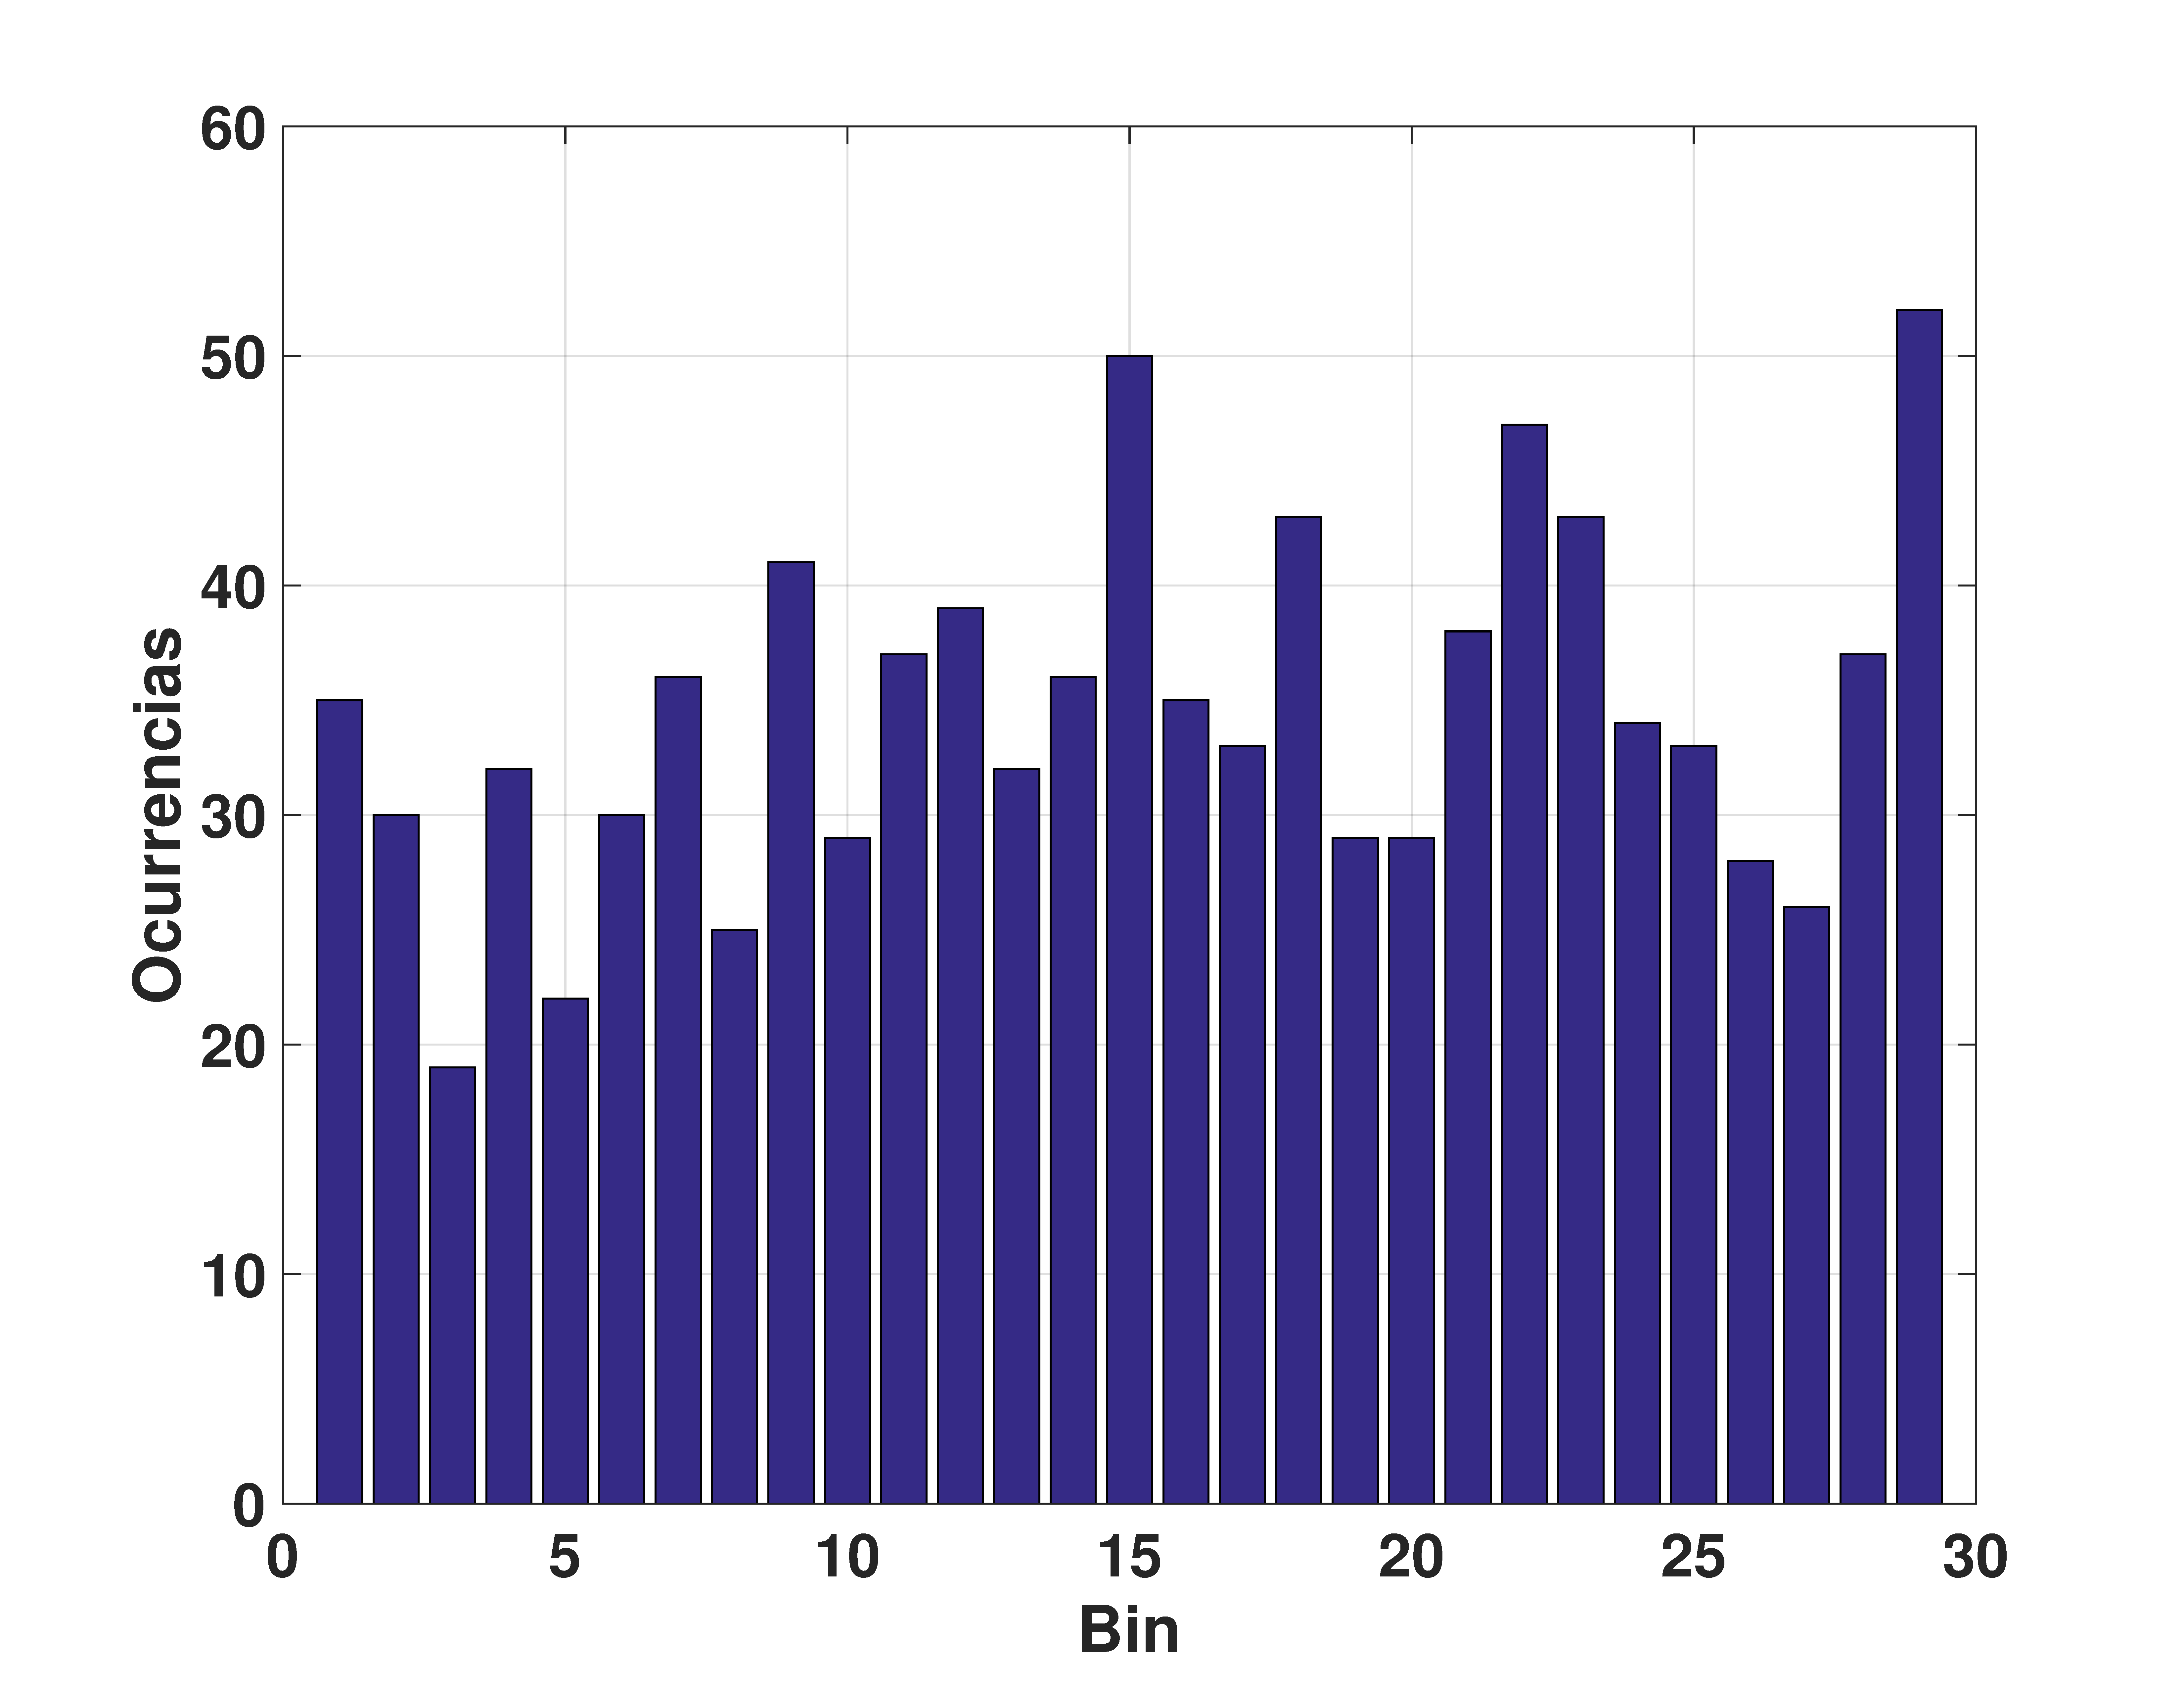
\includegraphics[width=\textwidth]{HistVal_y}
		\caption{Histograma de valores de los puntos ordenados}
		\label{subfig:causal_nocausal_HistValy}
	\end{subfigure}
	\begin{subfigure}[t]{0.49\textwidth}
		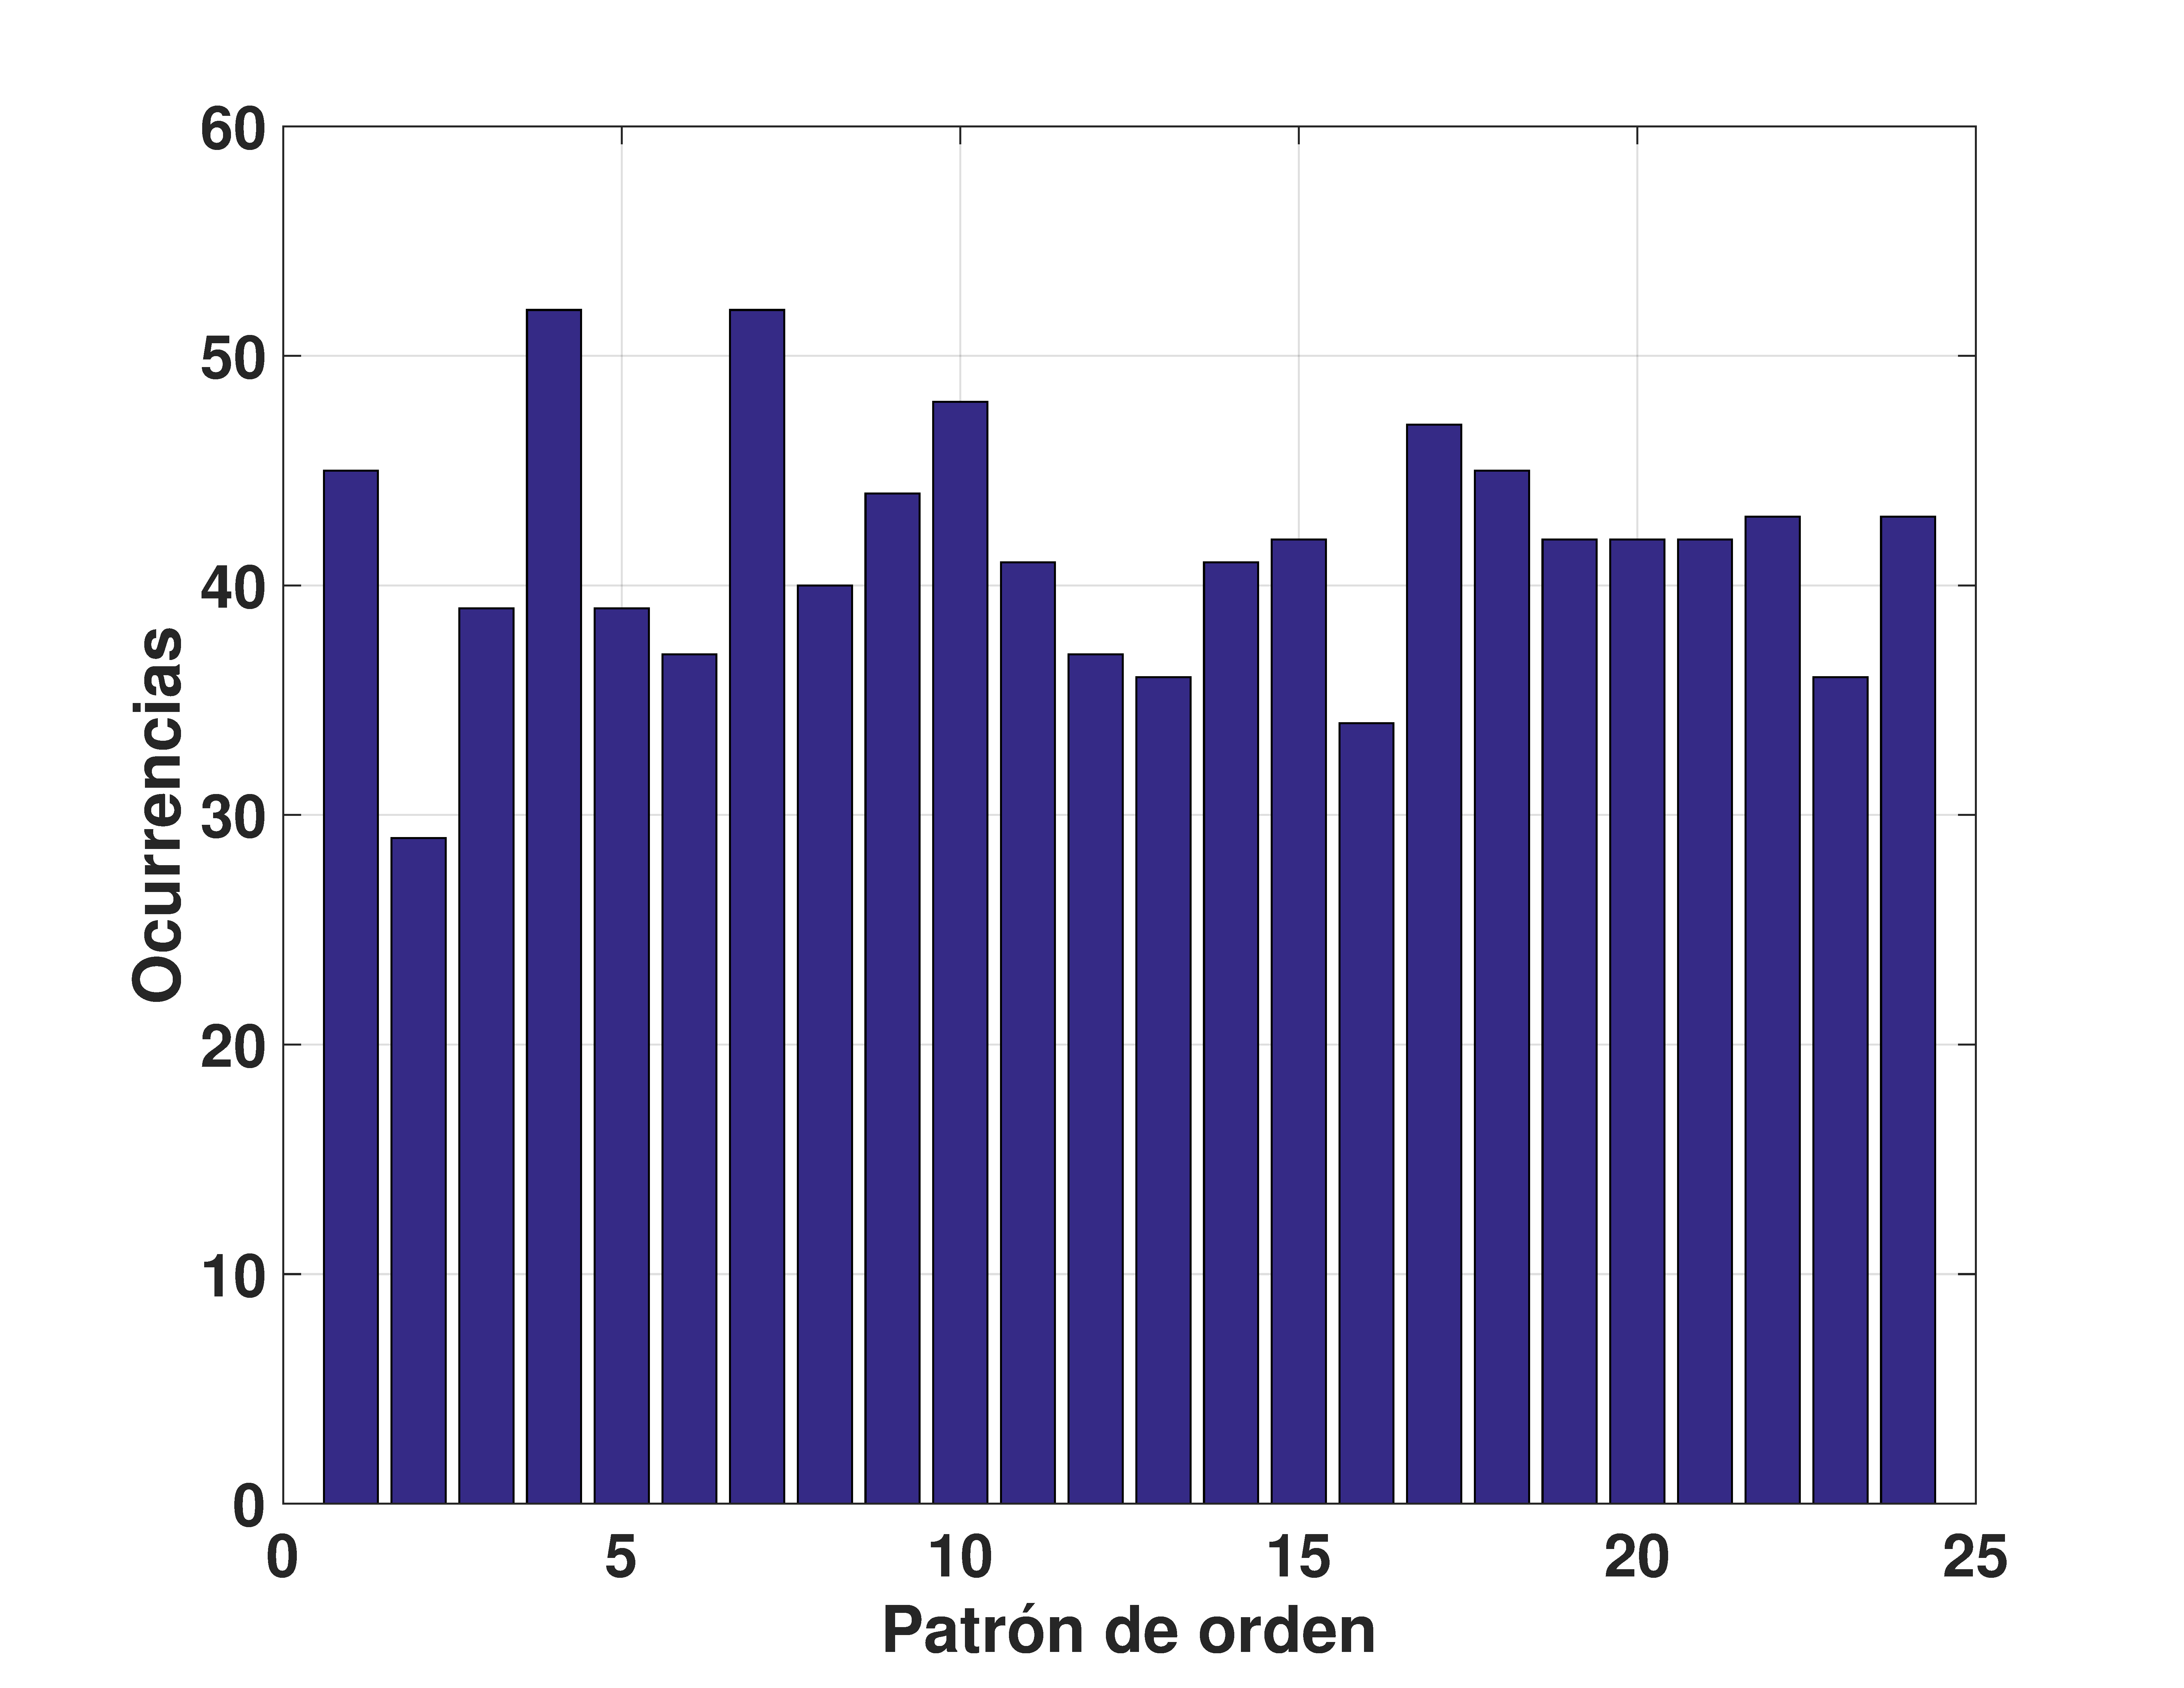
\includegraphics[width=\textwidth]{HistBP_x}
		\caption{Histograma de patrones de orden de los puntos sin ordenar}
		\label{subfig:causal_nocausal_HistBPx}
	\end{subfigure}
	\begin{subfigure}[t]{0.49\textwidth}
		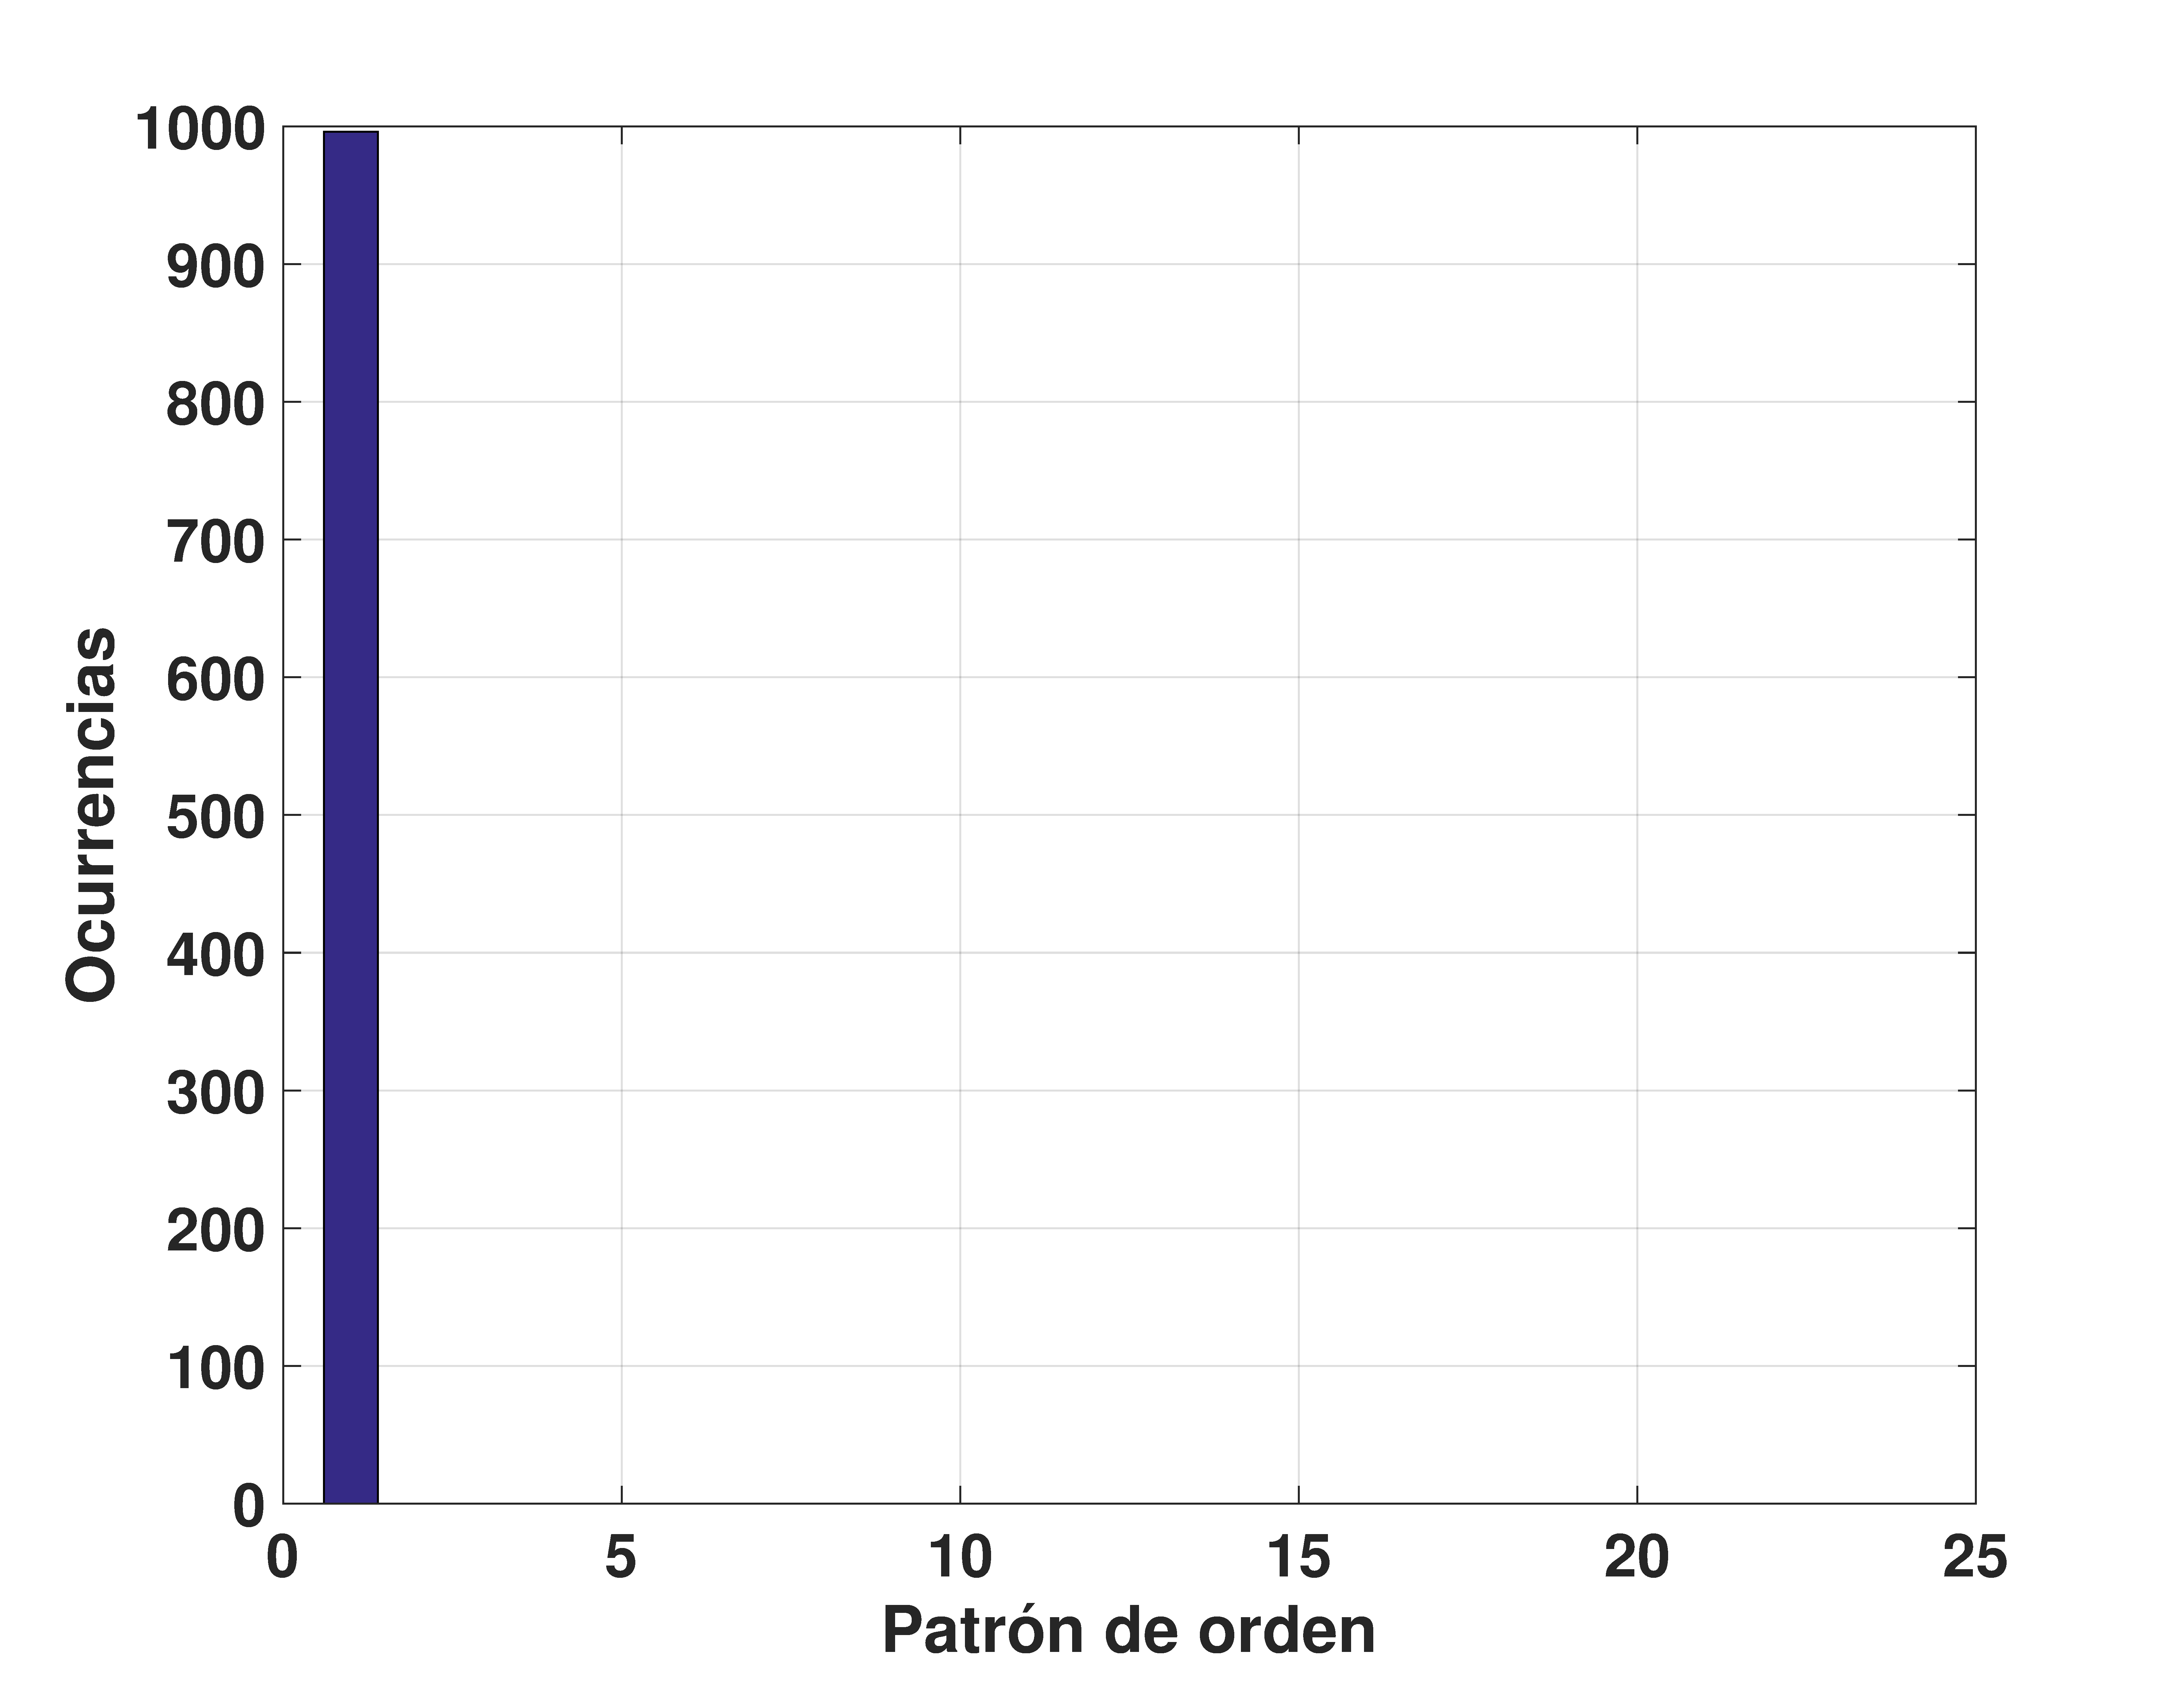
\includegraphics[width=\textwidth]{HistBP_y}
		\caption{Histograma de patrones de orden de los puntos ordenados}
		\label{subfig:causal_nocausal_HistBPy}
	\end{subfigure}
	\caption{Comparación entre histogramas causal y no causal}\label{fig:causal_nocausal}
\end{figure}

Recientemente, la entropía de permutación se amplió para incorporar también información de amplitud.
Ponderar las probabilidades de patrones individuales de acuerdo a su varianza mitiga los problemas potenciales con respecto a los patrones de "alto ruido, baja señal", porque los patrones de baja varianza que están fuertemente afectados por el ruido se ponderan en las distribuciones de patrones ordinales ponderados resultantes.
Por lo tanto, una posible desventaja de las estadísticas de los patrones ordinales, es decir, la pérdida de información de amplitud, se puede abordar mediante la introducción de pesos con el fin de obtener una "entropía de permutación ponderada (WPE)" \cite{Fadlallah2013}.
Los pesos no normalizados se calculan para cada ventana temporal para la serie de tiempo $X$, tal que
\begin{equation}
\label{WPE_weigth}
w_j~=~\frac{1}{D}\sum_{k=1}^{D} \left(x_{j+k-1}-\bar{X_j^D}\right)^2.
\end{equation}
En la ecuación anterior $x_{j+k-1}-\bar{X_j^D}$ denota la media aritmética del actual vector de embedding de longitud $D$ y su varianza $w_j$ se utiliza entonces para ponderar las frecuencias relativas de cada patrón ordinal $p_j$.
Originalmente, se propuso esta técnica para discriminar patrones sumergidos en un bajo nivel de ruido.
Nosotros también aprovechamos el hecho de que los puntos fijos no se computan en el WPE.

Al calcular la entropía de Shannon normalizada $H$ y la complejidad estadística $C$ de estas PDFs, y los valores obtenidos se denotan como:
\begin{itemize}
	\item $H_{hist}$, es la entropía de Shannon normalizada aplicada a una PDF no causal $P_{hist}$
	\item $H_{BP}$, es la entropía de Shannon normalizada aplicada a una PDF causal $P_{BP}$
	\item $H_{BPW}$,es la entropía de Shannon normalizada aplicada a una PDF causal con contribuciones de aplitud $P_{BPW}$
	\item $C_{BP}$, es la complejidad estadística normalizada aplicada a una PDF causal $P_{BP}$
	\item $C_{BPW}$, es la complejidad estadística normalizada aplicada a una PDF causal con contribuciones de amplitud $P_{BPW} $
\end{itemize}

\subsection{Planos deoble entropía y entropía-complejidad}

Una visualización particularmente útil de los cuantificadores de la Teoría de la Información es su yuxtaposición en los gráficos bidimensionales.
Se definen cuatro planos de información:
\begin{enumerate}
	\item Entropía causal vs. entropía no-causal, $H_{BP} \times H_{hist}$
	\item Entropía causal con contribución de amplitudes vs. entropía no-causal, $H_{BPW} \times H_{hist}$
	\item Complejidad causal vs. entropía causal, $C_{BP} \times H_{BP}$
	\item Complejidad causal con contribución de amplitudes vs. entropía causal con contribución de amplitudes, $C_{BPW} \times H_{BPW}$
\end{enumerate}

Estas herramientas de diagnóstico demostraron ser particularmente eficientes para distinguir entre el caos determinista y la naturaleza estocástica de una serie de tiempo ya que los cuantificadores de permutación tienen comportamientos distintos para diferentes tipos de procesos.

En la Fig. \ref{fig: HH} se muestran los planos $H_ {BP} \times H_{hist}$ y $H_{BPW} \times H_{hist}$ colapsados en un mismo plano.
En este plano un valor más alto en cualquiera de las entropías, $H_{BP}$, $H_{BPW}$ o $H_{hist}$, implica una mayor uniformidad de la PDF implicada.
El punto $(1, 1)$ representa el caso ideal con histograma uniforme y distribución uniforme de los patrones de orden.
Mostramos algunos puntos relevantes como ejemplo.

El ruido aleatorio blanco ideal con distribución uniforme da un punto en $(H_{hist}, H_{BP}) = (1, 1)$ representado por un círculo azul, un círculo rojo en la misma posición muestra los resultados cuando se incluyen las contribuciones de amplitud $(H_{hist}, H_{BPW}) = (1, 1)$.
Si ordenamos el vector ideal con distribución uniforme de forma ascendente, los puntos resultantes se muestran con un cuadrado azul $(H_{hist}, H_{BP}) = (1, 0)$ y un cuadrado rojo $(H_{hist}, H_{BPW}) = (1, 0)$, este ejemplo ilustra la complementariedad de $H_{hist}$ y $H_{BP}$.

Las estrellas azules y rojas muestran $(H_{hist}, H_{BP})$ y $ (H_{hist}, H_{BPW})$ respectivamente aplicadas a una señal de diente de sierra.
Los valores están perfectamente distribuidos en todos los intervalos, pero sólo aparecen unos pocos patrones de orden, esto explica el alto $H_ {hist}$ y bajo $H_ {BP}$.
La frecuencia de aparición de patrones de baja amplitud es mayor que los patrones de alta amplitud, entonces la PDF con contribuciones de amplitud es más uniforme y $H_ {BPW}$ es un poco más alto que $H_ {BP}$.
Cuando la señal de diente de sierra está contaminada con ruido blanco, se incrementan $H_ {BP}$ y $H_ {BPW}$ como se muestra con triángulos azules y rojos.
Es evidente que aparecen nuevos patrones de orden y tanto $H_{BP}$ como $H_{BPW}$ muestran valores más altos que los casos no contaminados, sin embargo el incremento de $H_{BPW}$ es menor que $H_{BP}$ mostrando que la técnica de registrar contribuciones de amplitud añade alguna inmunidad al ruido.

Finalmente, se evaluaron los cuantificadores de una secuencia de un mapa logístico que converge a un punto fijo, en todos los casos la longitud del vector de datos permanece constante y la longitud de transitorio es variable.
Los resultados obtenidos sin las contribuciones de amplitud se representan en puntos azules, convergen a $(H_{hist}, H_{BP}) = (0, 0)$ a medida que la longitud de transitorio se hace más corta, sin embargo $H_{BPW}$ (puntos rojos) permanece constante para todos los casos.
El último punto en $(H_{hist}, H_{BP}) = (0, 0)$ corresponde a un vector de ceros, en este caso el histograma de patrones de orden con contribuciones de amplitud es también un vector nulo y $H_{BPW}$ no se puede calcular.
A través de este último ejemplo, mostramos que la convergencia a un punto fijo puede ser detectada por la información conjunta de $H_{BP}$ y $H_{BPW}$.

En la figura \ref{fig:HC} se muestra el plano causal $H_{BP} \times C_{BP}$.
Podemos ver que no toda la región $0 < H_{BP} < 1$, $0 < C_{BP} < 1$ es alcanzable, de hecho, para cualquier PDF los pares $(H, C)$ de valores posibles caen entre dos curvas extremas en el plano $H_{BP} \times C_{BP}$ \ cite {Anteneodo1996}.
Los mapas caóticos tienen entropía intermedia $H_{BP}$, mientras que su complejidad $C_{BP}$ alcanza valores mayores, muy cercanos a los del límite de complejidad superior \cite{Rosso2007, Olivares2012}.
Para procesos regulares, la entropía y la complejidad tienen valores pequeños, cercanos a cero.
Los procesos estocásticos no correlacionados se ubican en la localización planar asociada con $H_{BP}$ cerca de uno y $C_{BP}$ cerca de cero.
Los sistemas aleatorios ideales que tienen un Bandt \& Pompe PDF uniforme, están representados por el punto $(1,0)$ \ cite{Gonzalez2005} y una PDF tipo delta corresponde al punto $(0,0)$.

En la figura \ref{fig:HC} mostramos $H_{BP} \times C_{BP}$ con y sin contribuciones de amplitud.
Se muestran los mismos puntos de muestra para ilustrar las posiciones planas para diferentes vectores de datos.

En ambos planos de información $H_ {BP} \times H_ {hist}$ en la Fig. \ref{fig:HH} y $H_{BP} \times C_{BP}$ en Fig. \ref{fig:HC}, los datos estocásticos, caóticos y deterministas están claramente localizados en diferentes posiciones planares.

\begin{figure}[htpb]
	\centering	
	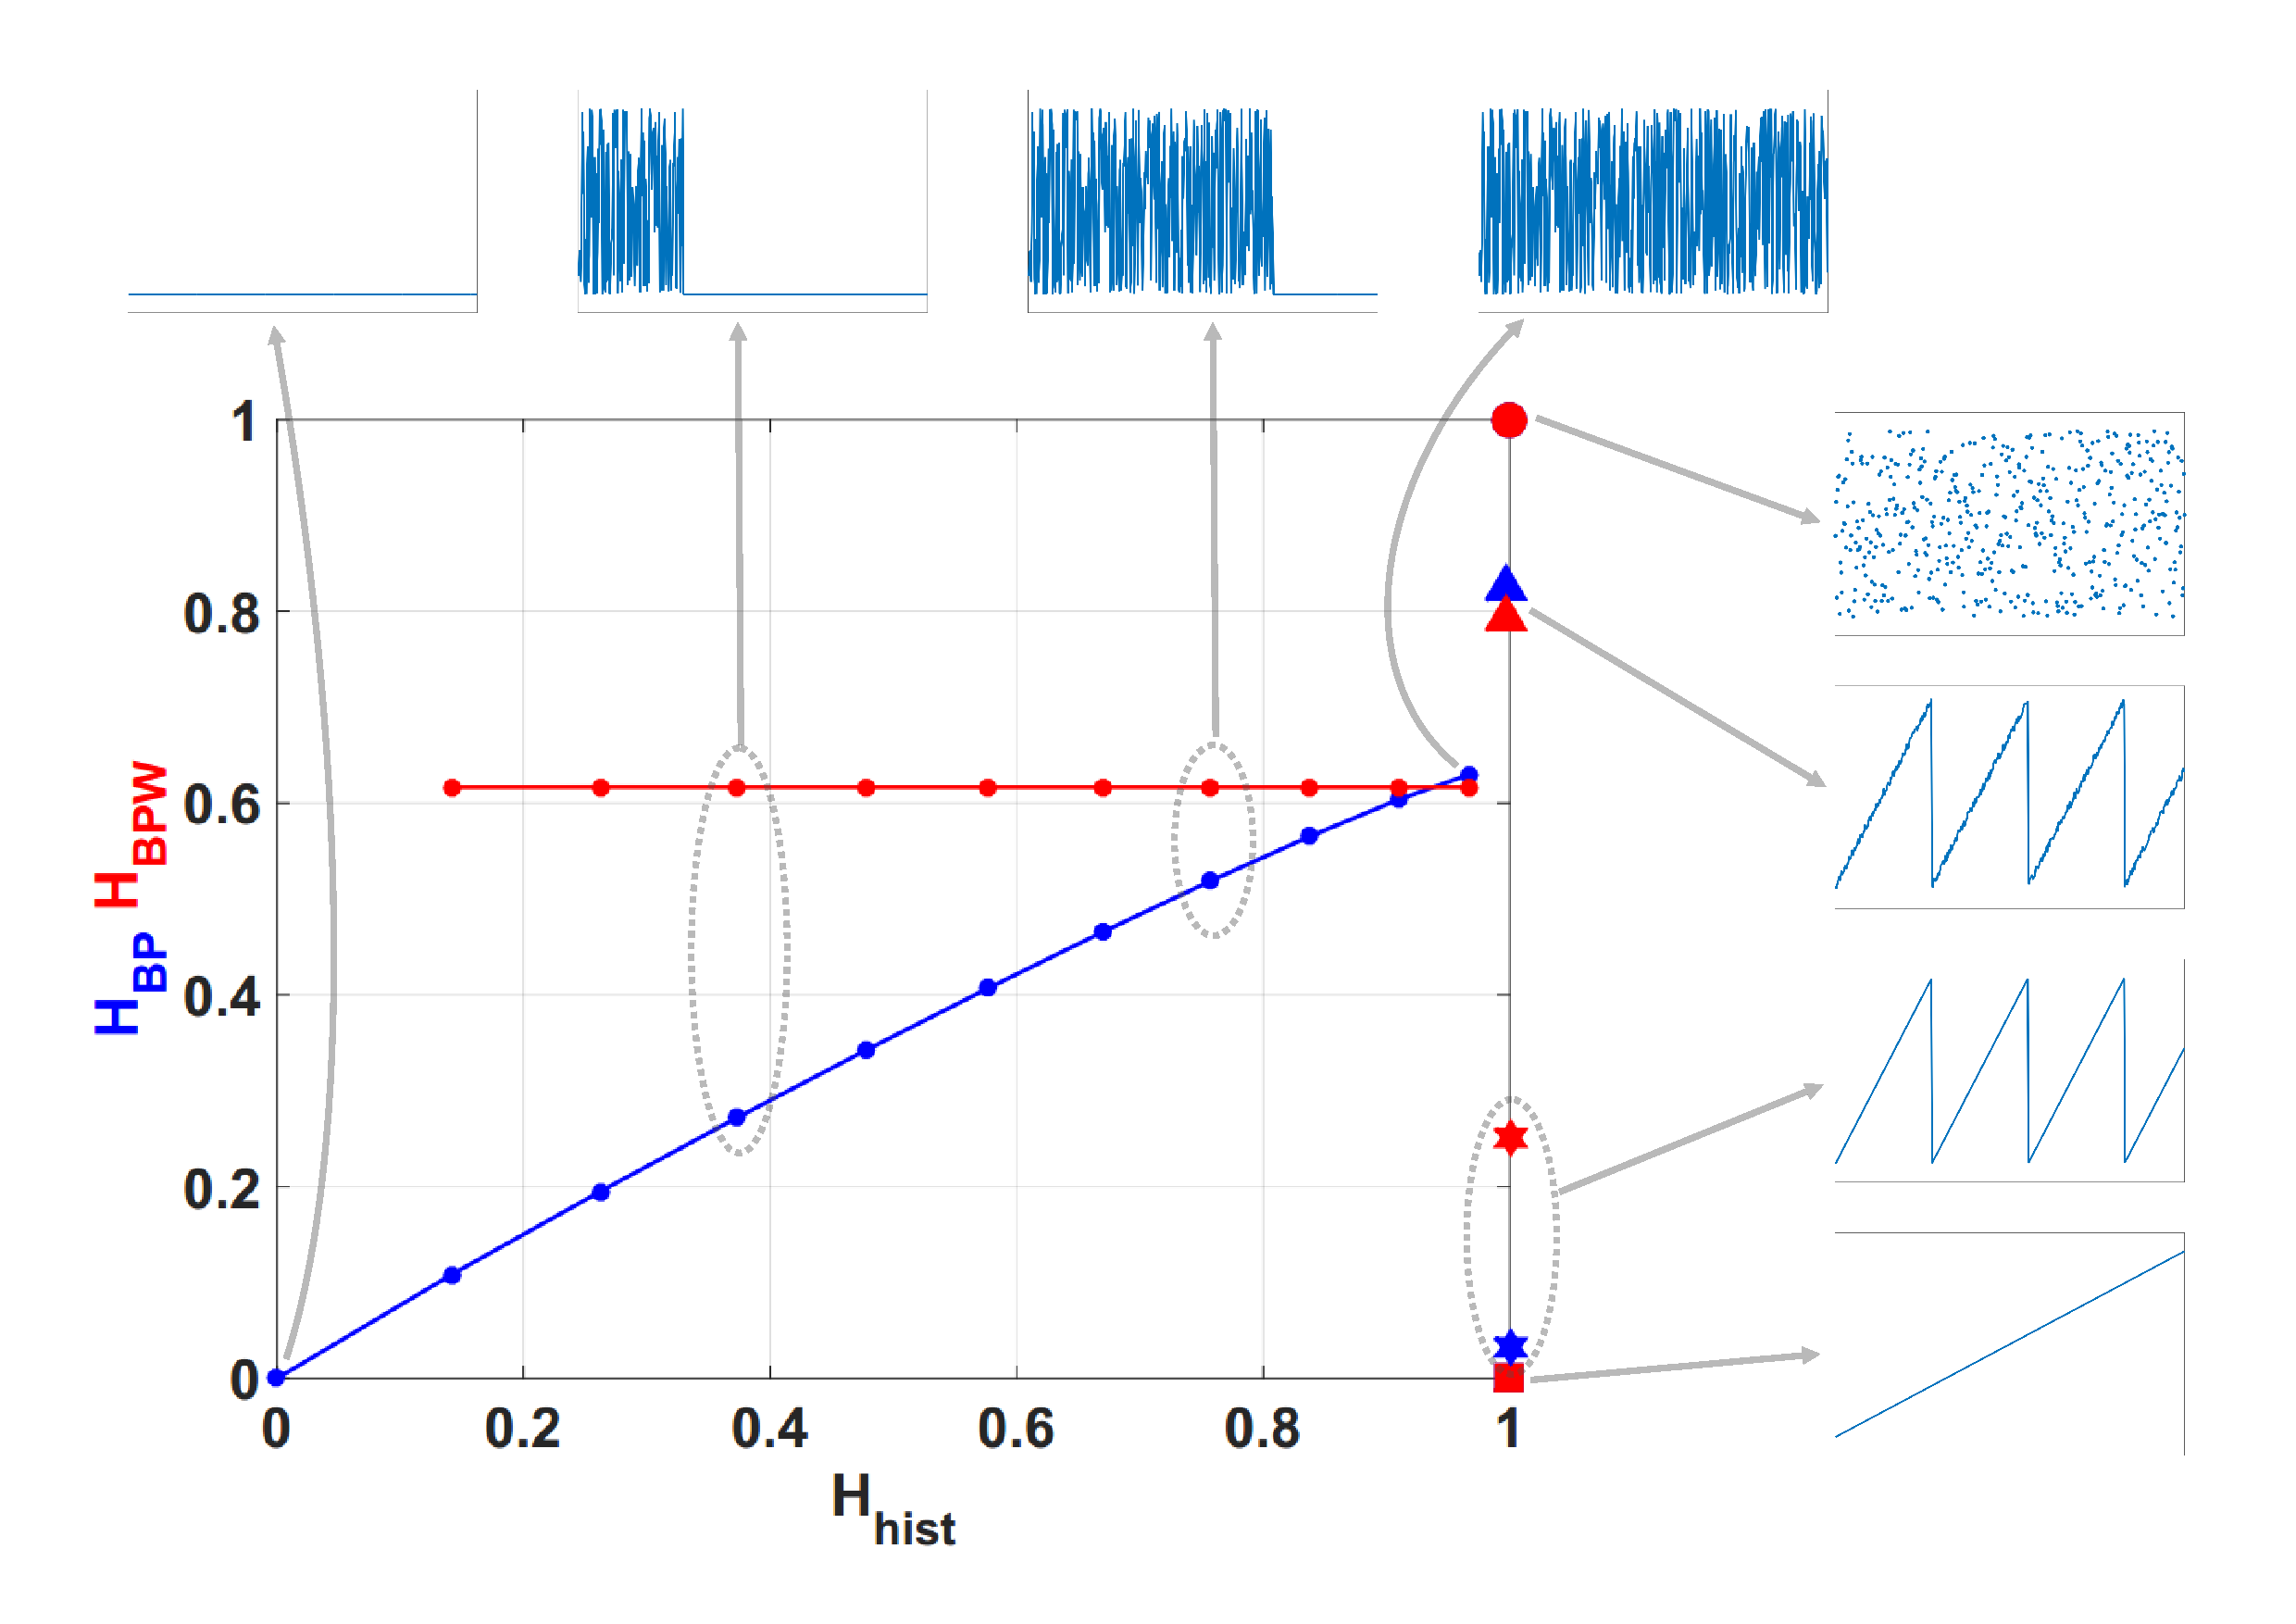
\includegraphics[width= .99\textwidth]{Fig1HHSignals}
	\caption{Causal-Non causal Entropy plane.}
	\label{fig:HH}
\end{figure}

\begin{figure}[htpb]
	\centering		
	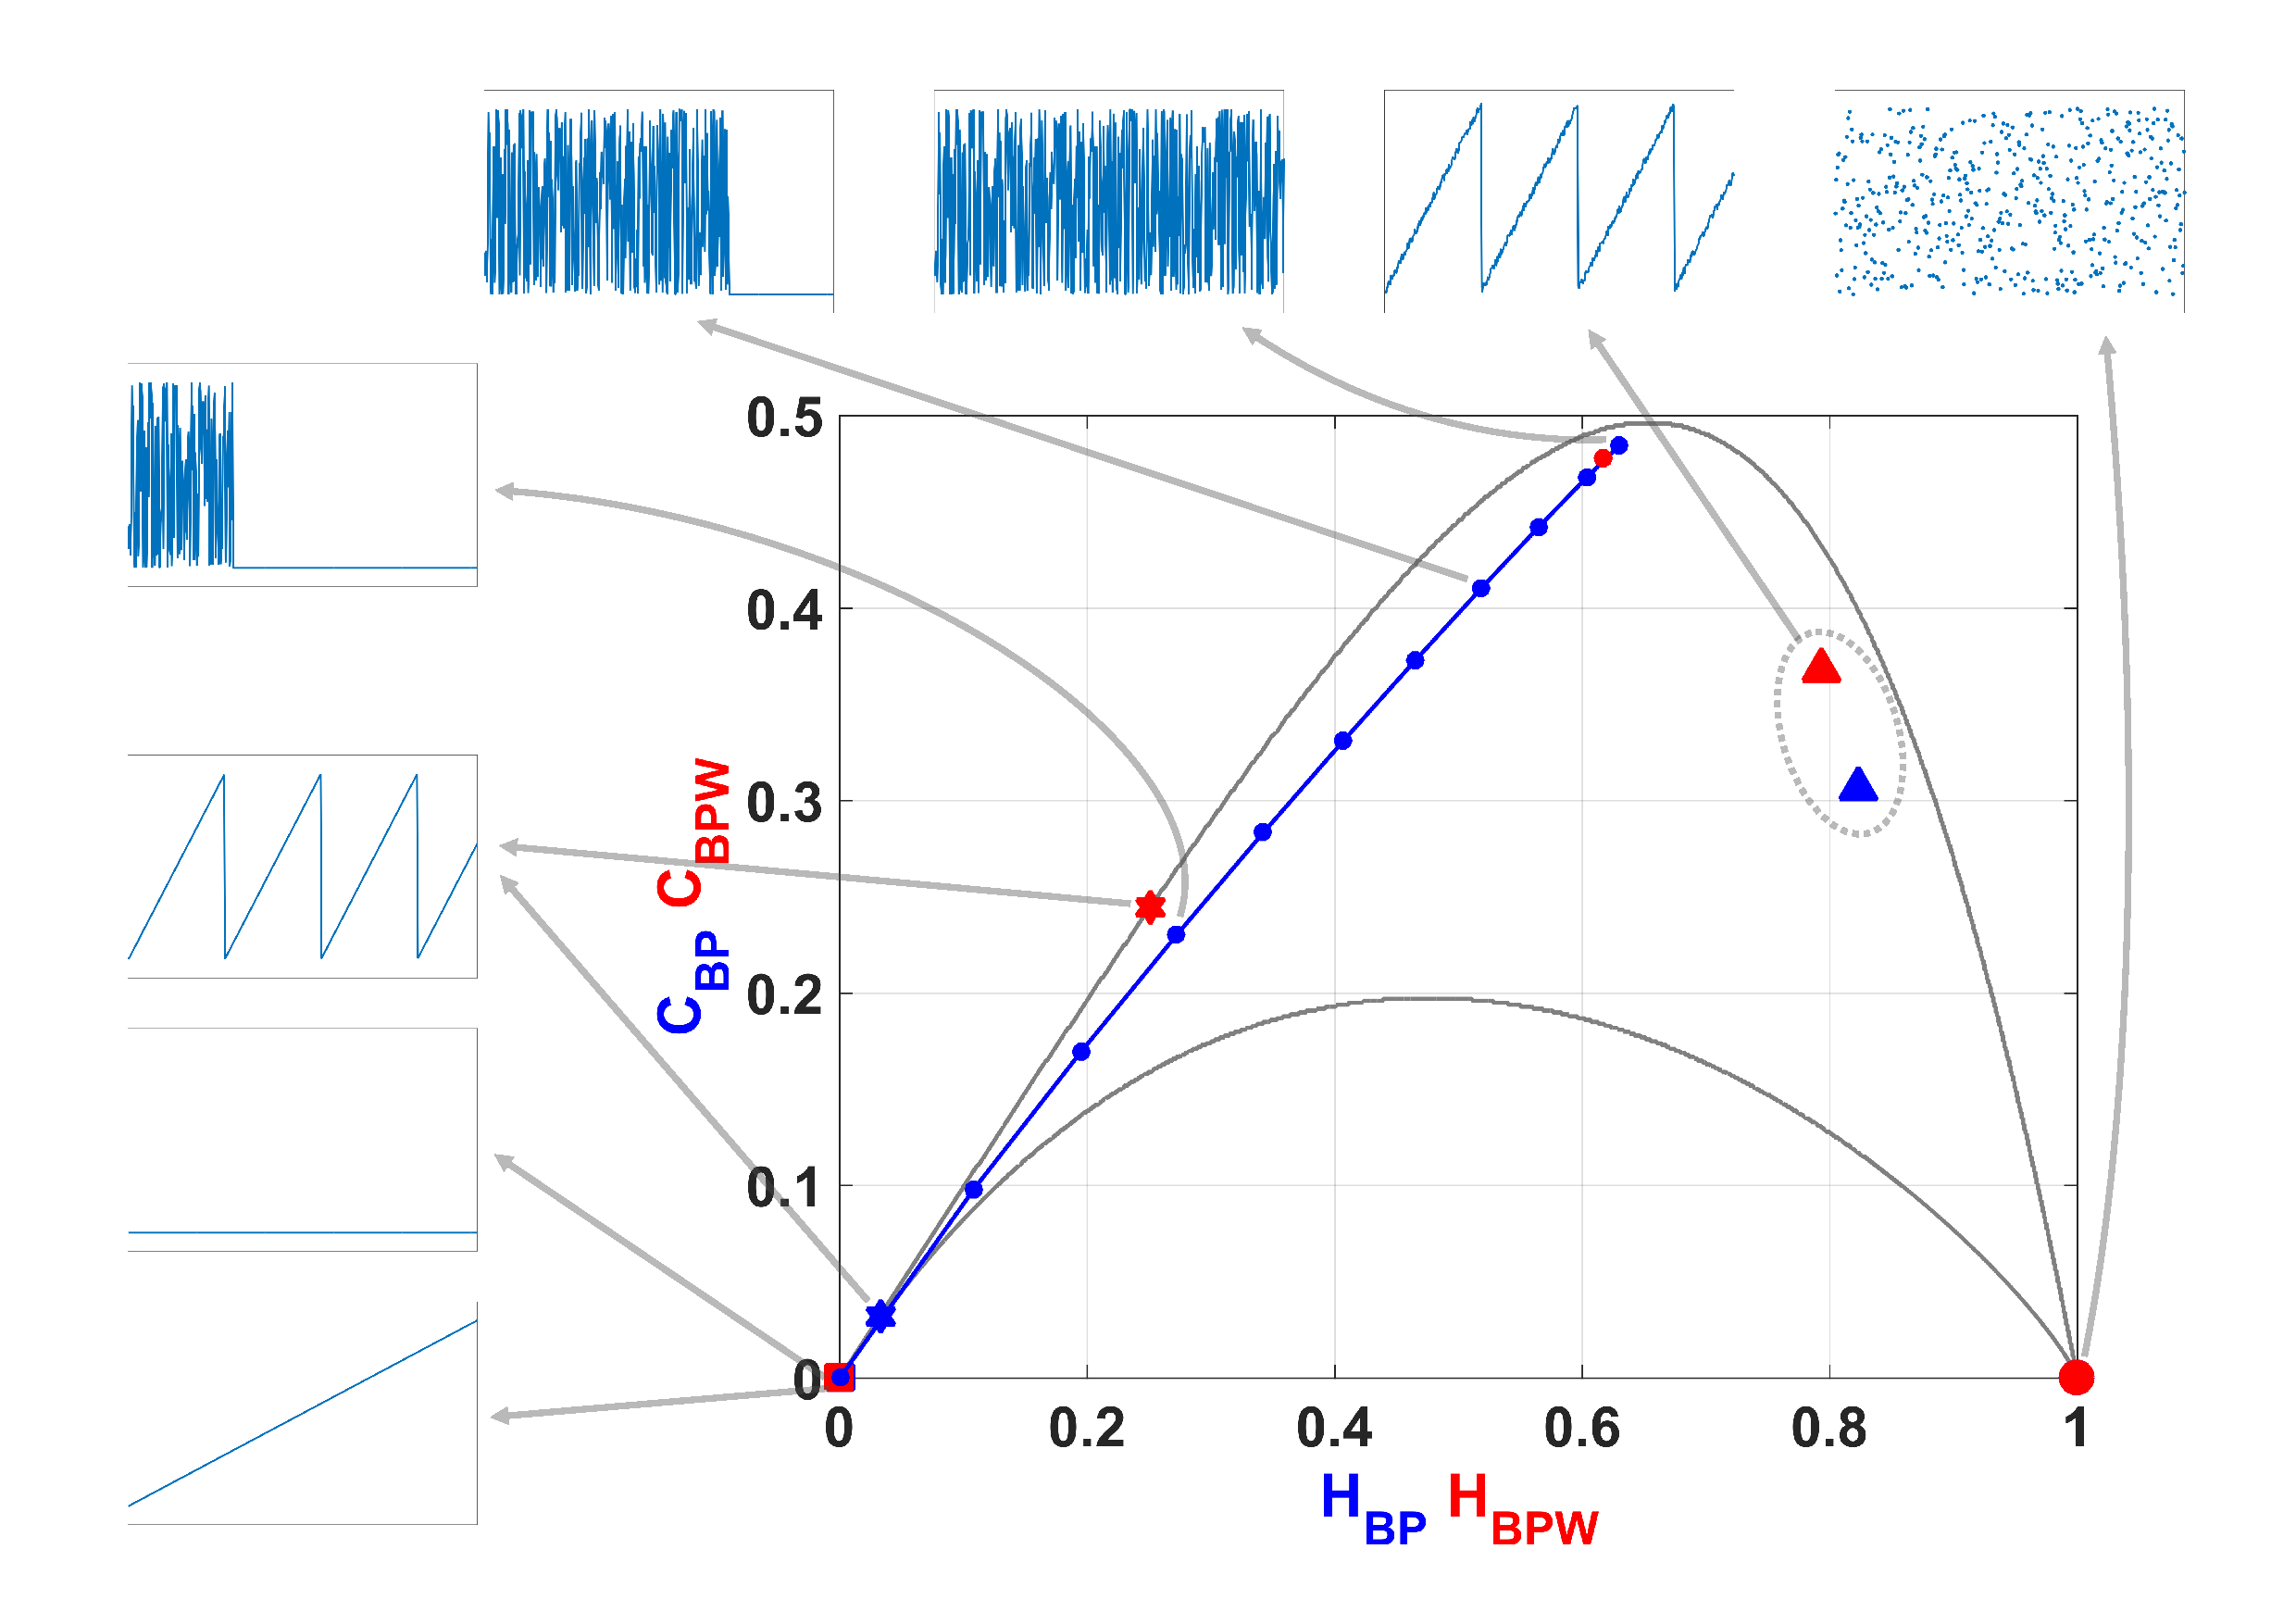
\includegraphics[width= .99\textwidth]{Fig1HCSignals}
	\caption{Causal Entropy-Complexity plane.}
	\label{fig:HC}
\end{figure}

También usamos el número de patrones perdidos MP como un cuantificador \cite {Rosso2012}.
Como mostraron recientemente Amigó y colaboradores \cite{Amigo2006,Amigo2007,Amigo2008,Amigo2010}, en el caso de mapas deterministas, no todos los patrones de orden posibles pueden materializarse efectivamente en órbitas.
De hecho, la existencia de estos patrones de orden faltantes se convierte en un hecho persistente que puede considerarse como una nueva propiedad dinámica.
Por lo tanto, para una longitud de patrón fija (dimensión de embedding $D$) el número de patrones perdidos de una serie temporal (patrones no observados) es independiente de la longitud de la serie $N$.
Obsérvese que esta independencia no caracteriza otras propiedades de la serie como la proximidad y la correlación \cite{Amigo2007,Amigo2010}.

\subsection{Entropías diferenciales}
\label{subsec:addquanti}

La entropía de Shannon $S(P)$ es el punto de partida para otros cuantificadores.

!!!!HABLAR DE LOS CONJUNTOS DE PARTICIONES Y NO SE QUE!!!

Para medir la entropía de una serie binaria es necesario 

!!!FIN DE HABLAR DE LOS CONJUNTOS DE PARTICIONES Y NO SE QUE!!!

\begin{enumerate}
	\item Entropía normalizada $H(P)$: es la entropía de Shannon dividida por su valor máximo. Por ejemplo, si usamos $S_2$ (ver arriba), se obtiene la entropía máxima para equiprobabilidad entre dos símbolos. Su valor es $S_{max}=-1/2 log(1/2)-1/2 log(1/2)=log(2)=1$; tentonces, la entropía normalizada es $H_2=S_2$. Si usamos $S_W$ la equiprobabilidad entre las $2^W$ posibles palabras (números decimales de $W$-bits) produce $S_{max}=W$ y $H_W=S_W/W$. Finalmente, para $S^{(D)}_{BP}$ la equiprobabilidad entre los $D!$ patrones de orden produce $S_{max}= log(D!)$ y $H^{(D)}_{BP}=S^D_{BP}/log(D!)$.
	\item Entropía diferencial o condicional $h$ y $h^*$ son:
	\begin{eqnarray}
	h~=~S_{W+1}-S_W\\
	h^*~=~S_{BP}^{(D+1)}-S_{BP}^{(D)}
	\end{eqnarray}
	En las expresiones de arriba $W=1,2,...$ y $D=2,3,...$, $S_0=0$ y $S_{BP}^{(1)}=0$. Esta entropía diferencial o condicional da la cantidad promedio de información requerida para predecir el símbolo $(W+1)$ (o $(D+1)$), dado los $W$ (o $D$) símbolos precedentes.
	\item Finalmente, las \emph{rate entropies} $h_0$ y $h_0^*$ \cite{Ebeling2001,Amigo2005} son dadas por:
	\begin{eqnarray}
	h_0=\lim\limits_{W\rightarrow \infty} h=\lim\limits_{W\rightarrow \infty}{S_{W}/W }\\
	h^*_0= \lim\limits_{D\rightarrow \infty} h^*=\lim\limits_{D\rightarrow \infty}{S^{(D)}_{BP}/(D-1)}
	\end{eqnarray}
\end{enumerate}

Enfatizemos algunas cuestiones importantes involucradas en los cálculos de las entropías binarias mencionadas anteriormente:
\begin{enumerate}
	\item La entropía binaria $S_2$ es no causal, mientras que ambas, la entropía de bloque $S_W$ y la entropía Bandt \& Pompe $S^{(D)}_{BP}$, son causales.
	\item La entropía de bloque $S_W$ tiene en cuenta las correlaciones entre $W$ bits consecutivos.
	La entropía Bandt \& Pompe $S^{(D)}_{BP}$ tiene en cuenta las correlaciones entre $D$ consecutivas palabras de longitud $W$.
	Ambos procedimientos de agrupación (números decimales de $W$ bits y patrones de permutación de $D$ números decimales) pueden realizarse con o sin superposición.
	La cantidad de datos requeridos para obtener buenas estadísticas es diferente dependiendo de que los procedimientos de agrupación se realicen.
	\item Para $ S_W $ solo hay un proceso de agrupación ($W$ bits agrupados para obtener una serie de números decimales $Y$).
	Definamos $\alpha$ como un parámetro de calidad estadística, dado por el cociente entre el número de elementos en la serie de tiempo simbólica $Y$ y la cantidad de símbolos en el alfabeto.
	En este documento, no aceptaremos $\alpha < 10$.
	
	Obviamente, el factor de calidad $\alpha$ aumenta con la longitud de la serie temporal:
	%
	\begin{enumerate}
		\item si el agrupamiento de $W$ bits está hecho con, dos palabras consecutivas de longitud $W$ comparten $W-2$ bits.
		En consecuencia, comenzando con un archivo con una longitud de $N$ bits obtenemos $N - W + 1$ palabras.
		Además, hay símbolos $2 ^ W$ en el alfabeto y $\alpha = (N - W + 1) / (2 ^ W)$.
		\item Si $S_W$ se evalúa sin superposición la cantidad de palabras de longitud $W$ es $floor\{N/W\}$ y el parámetro de calidad se calcula como $\alpha=floor~\{N/W\}/(2^W)$.
		Si $N \gg W$ el factor de calidad estadística es $W$ veces más bajo que el usado con superposición.
	\end{enumerate}
	
	\item En el caso de $S^{(D)}_{BP} $, hay dos procesos de agrupación involucrados.
	\begin{enumerate}
		\item Si ambos procesos de agrupamiento se realizan con superposición obtenemos $NW-D + 2$ elementos comenzando con un archivo $ N $ bits de longitud, y el factor de calidad es $\alpha = (NW-D + 2) / D!$.
		En este caso $S ^ {(D)}_{BP}$ tiene en cuenta las correlaciones entre $W + D$ bits consecutivos.
		\item Si el proceso de agrupación de $W$ bits se realiza sin superposición pero la agrupación de números decimales $D$ se realiza con superposición obtenemos $floor\{N/W\}-D+1$ elementos y el parámetro de calidad estadística es $\alpha=(floor\{N/W\}-D+1)/D!$.
		En este caso $S^{(D)}_{BP}$ incluirá correlaciones entre $WD$ bits consecutivos.
		\item Si el proceso de agrupación de $W$ bits se realiza con superposición y la agrupación de números decimales $D$ se realiza sin superposición, obtenemos $floor\{(N-W+1)/D\}$ elementos a partir de un archivo de $N$ bits.
		El factor de calidad estadística es $\alpha=floor\{(N-W+1)/D\}/D!$ y $S^{(D)}_{BP}$ tiene en cuenta correlaciones de $W+D-1$ bits.
		\item Si ambos procesos de agrupación se realizan sin superposición, obtenemos $floor\{floor\{N/W\}/D\}$ elementos a partir de un archivo de longitud de  $N$ bits.
		El factor de calidad estadística es $\alpha=floor\{floor\{N/W\}/D\}/D!$ y $S^{(D)}_{BP}$ tiene en cuenta las correlaciones entre $WD$ bits consecutivos.
	\end{enumerate}
\end{enumerate} 
\subsection{Cuantificador de Entropías Implementado en FPGA}
\label{ssecCuantiImpFPGA}

En esta Sección se describe la implementación de un sistema de medición de entropías.
El diseño fue optimizado para ser implementado en un microcontrolador simple y pequeño, conservando una precisión aceptable.
El sistema permite medir entropías a señales generadas internamente por código y a señales externas analógicas muestreadas.
Se utilizó la placa de desarrollo \textit{M1AFS-embedded kit} de ACTEL.
En la FPGA (\textit{Field Programmable Gate Array}) se instanció un microcontrolador 8051 al que se programó en lenguaje C.
Se detalla el diseño del \textit{hardware} y \textit{software} y los resultados obtenidos.
Al momento hay muy poca bibliograf\'ia sobre implementaciones en \textit{hardware} de estos cuantificadores \cite{DeMicco2013}.

La entropía es empleada en diversas aplicaciones, como por ejemplo, en la detección de anomalías en flujos de datos IP \cite{Gu2005,Wagner2006, actelM1AFS1500}.
En \cite{Subramanya2008} se presentó un diseño y simulación en FPGA de un cuantificador de entropía, sin embargo, actualmente no hay disponibles implementaciones en \textit{hardware} de este cuantificador.

En esta tesis se implementó un sistema que calcula la entropía para la PDF asociada a una serie de datos.
Se analizan PDFs causales y no causales.
Los datos pueden tener un origen digital (generados mediante códigos), o bien provenir del muestreo de señales analógicas.
Se utilizó la placa de desarrollo \textit{M1AFS-embedded kit}, basado en el chip \textit{M1AFS1500} que se destaca por tener un bloque analógico embebido en el mismo encapsulado de la FPGA.
Luego, se verificó la exactitud numérica del cuantificador implementado comparando sus resultados con un programa patrón.
A partir del máximo error detectado se determinó la exactitud numérica del sistema.

\subsubsection{\textit{Hardware} Implementado}
\label{sec:Hardware}

El diseño del \textit{hardware} se basó en el que provee ACTEL en \cite{Core8051sH}, basado en el microcontrolador 8051, interfaces y periféricos.
Fue realizado con el paquete de programas \textit{Libero~Soc~v11.3\textsuperscript\copyright} de ACTEL.
Se utilizó la placa de desarrollo \textit{M1AFS-EMBEDDED-KIT} que contiene una FPGA \textit{M1AFS1500} de ACTEL y periféricos \cite{actelM1AFS1500}.
El chip \textit{M1AFS1500} contiene embebido un bloque analógico que consiste en nueve adaptadores direccionables de cuatro entradas cada uno, un multiplexor analógico de 32 entradas y un conversor analógico-digital configurable.

El sistema implementado puede dividirse en tres etapas principales como se muestra en la Figura \ref{Fig:Sistema}: una primera etapa de Adquisición de datos, que convierte a palabras digitales las señales del mundo analógico, una Lógica de Cálculo, que se vale de la memoria SRAM para llevar a cabo los cálculos y coordinar las interfaces y una etapa de Presentación de resultados, que envía los resultados de la medición a una computadora a través de la interfaz \textit{USB-to-UART}.
%
\begin{figure}
	\centering
	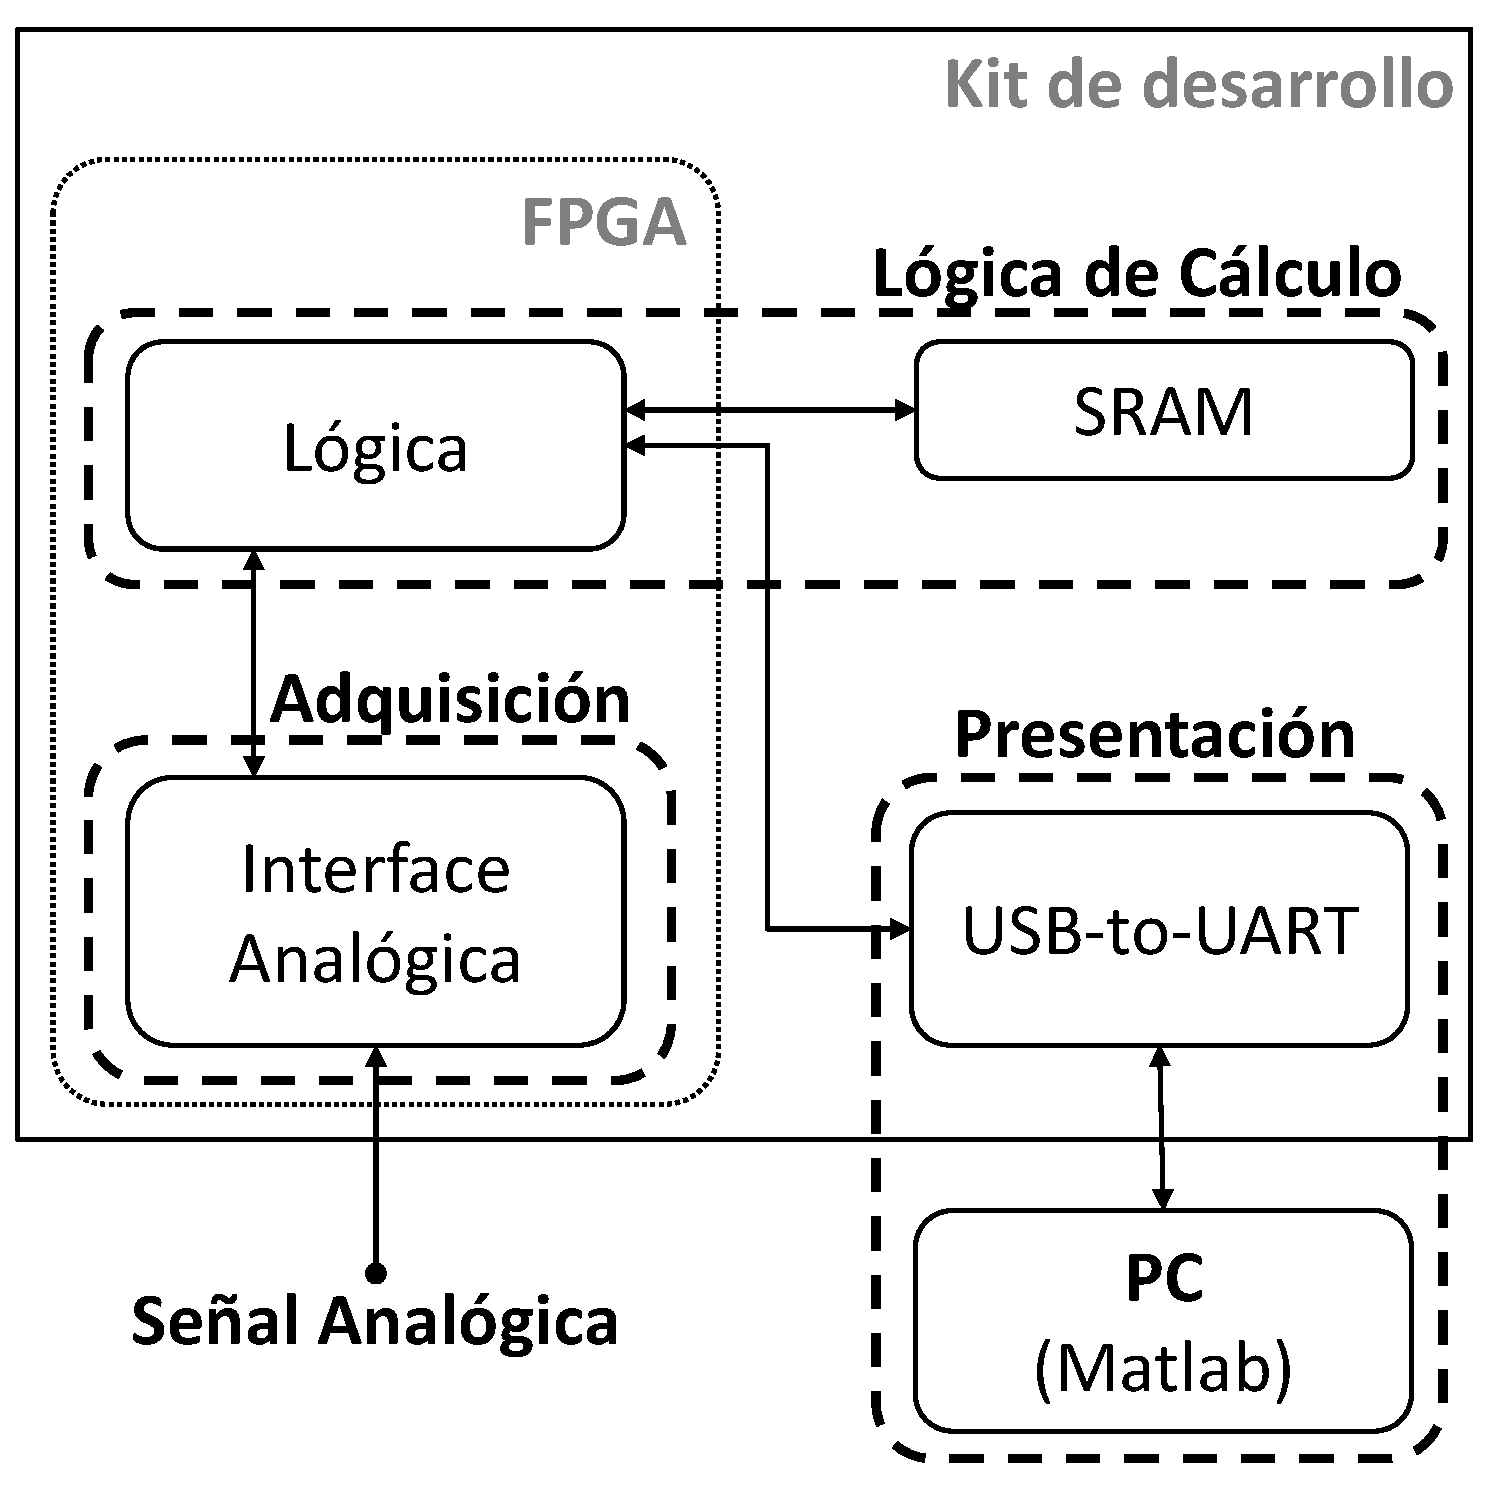
\includegraphics[width=.8\columnwidth]{Sistema.pdf}\\
	\caption{Esquema del sistema completo.}\label{Fig:Sistema}
\end{figure}

\begin{enumerate}
	\item \textit{Etapa de Adquisición:}
	
	Para ingresar los datos analógicos a ser evaluados utilizamos la entrada de tensión $AV2$ del \textit{Analog~Quad~2} del bloque analógico.
	Se encuentra direccionada en el canal siete del multiplexor analógico y fue configurada para un rango de tensiones de entrada de 0~V a 4~V.
	El conversor analógico-digital se configuró con una resolución de 12~bits.
	En este primer prototipo la frecuencia de muestreo máxima alcanzada fue de 16~ks/s limitada por el retardo necesario en el procesamiento de la lógica.
	
	\item \textit{Lógica de cálculo:}
	
	En esta etapa se realizan los cálculos y la sincronización entre periféricos.
	En la Figura \ref{fig:logica} pueden verse los bloques principales que la componen.
	%
	\begin{figure}
		\centering
		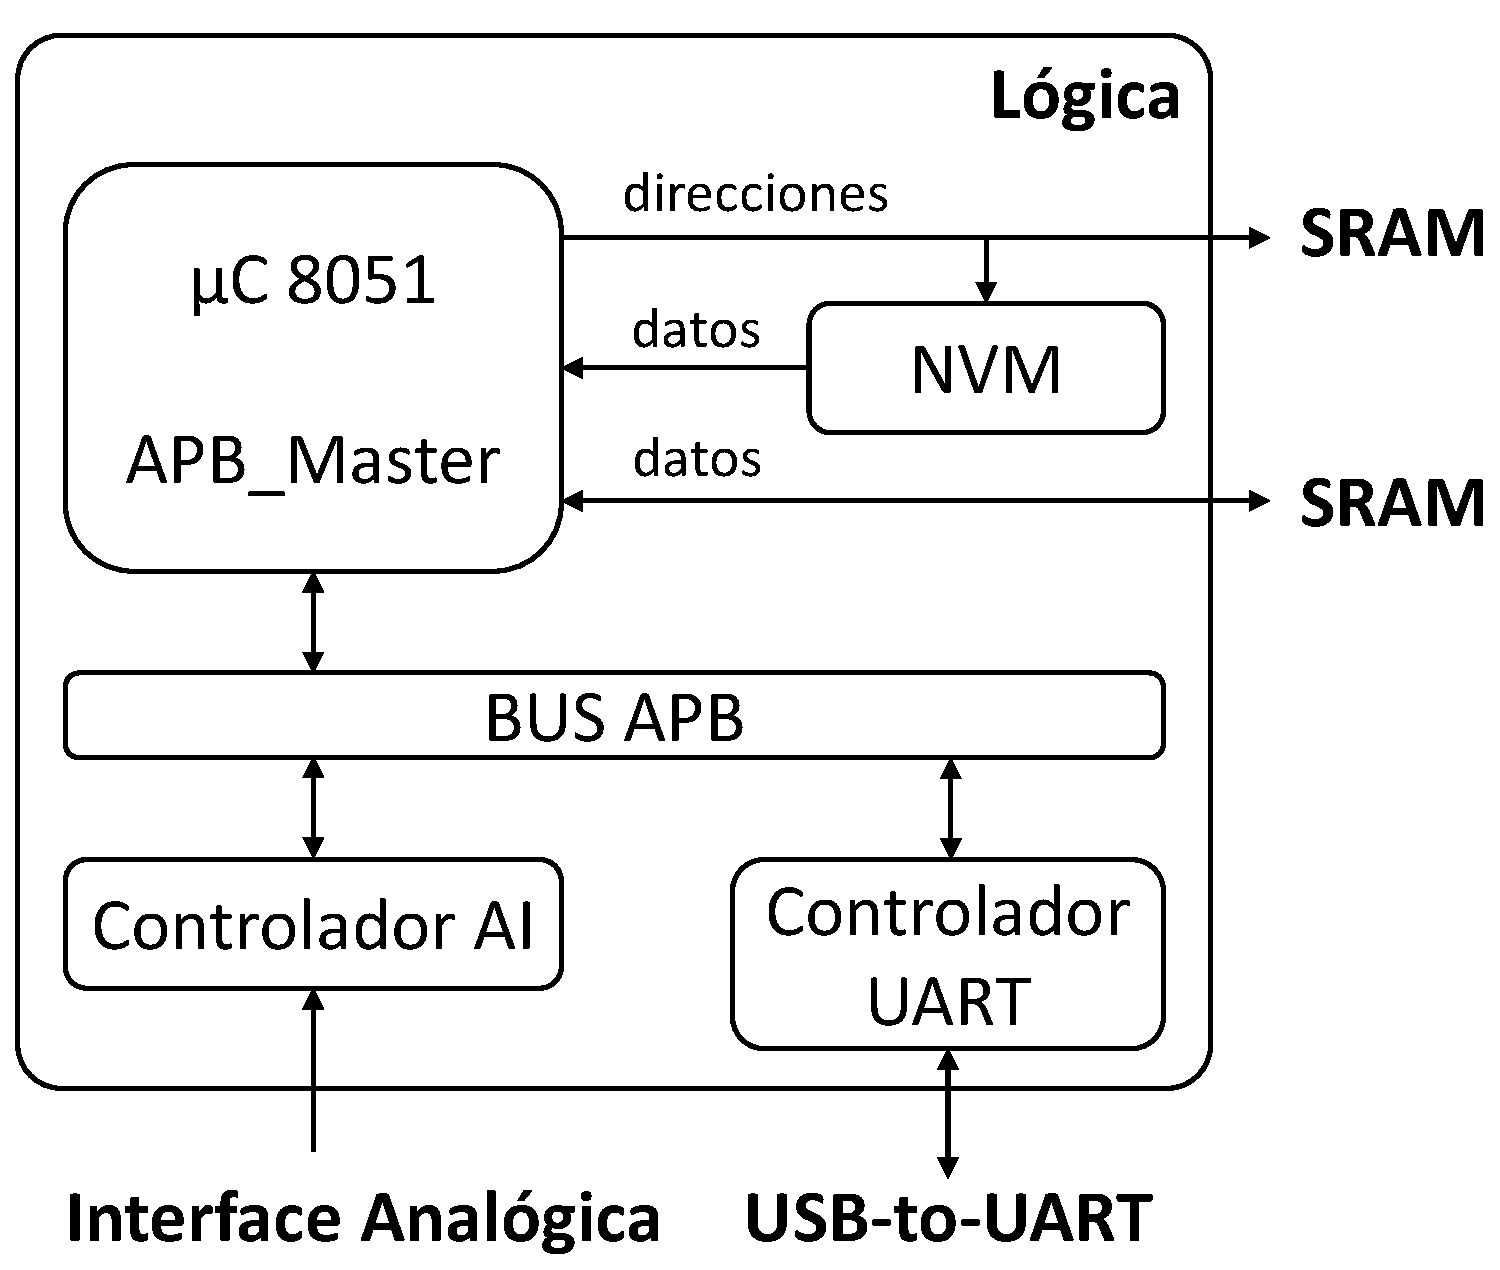
\includegraphics[width=.75\columnwidth]{Logica.pdf}\\
		\caption{Detalle de la lógica de cálculo.}\label{fig:logica}
	\end{figure}
	
	El núcleo de la implementación es un \textit{Core} 8051 que provee ACTEL en su catálogo de librerías.
	Se trata de un microcontrolador que contiene la lógica principal del microprocesador 8051 de Intel, sin sus periféricos.
	Este micro tiene una arquitectura Von Newman con un bus de direcciones de 16~bits, lo que limita nuestro diseño a $64~KB$ de memoria de código y $64~KB$ de memoria de datos.
	
	Sobre este microcontrolador corre el programa que realiza los cálculos presentados en la Sección \ref{sec:ITQs}.
	Se encarga de, a partir de los datos de entrada, obtener las PDFs ($BP$ e $hist$) y de realizar los cálculos para la obtención de las entropías, según la Ecuación \ref{shannon-disc-normalizada}.
	El \textit{software} implementado se describe más detalladamente en la Sección \ref{sec:Software}.
	
	La memoria de código es una memoria no volátil (NVM) implementada con los bloques flash internos de la FPGA.
	Ocupa las direcciones desde 0x0000 hasta 0xFFFF y se escribe con el contenido de un archivo en formato hexadecimal durante la compilación.
	
	Las funcionalidades del sistema son ampliadas mediante la conexión de periféricos a través de la interfaz APB.
	
	Para realizar la comunicación con la PC utilizamos el \textit{Controlador UART}.
	La salida de este bloque es dirigida hacia afuera de la FPGA y se conecta a un chip \textit{USB-to-UART} que se encuentra soldado a la placa del kit de desarrollo.
	
	El bloque analógico es controlado por el \textit{Controlador AI}, que direcciona y sincroniza sus entradas.
	
	\item \textit{Presentación:}
	
	La etapa de Presentación de los datos involucra al chip adaptador \textit{USB-to-UART} que se encuentra en la placa de desarrollo y es manejado tanto por el programa que corre en la FPGA como por el \textit{software} que corre sobre la PC.
	El chip adaptador \textit{USB-to-UART} es el responsable de adaptar la entrada-salida UART de la lógica a una entrada-salida USB estándar mediante la cual es posible interactuar con la PC.
	Por otra parte el programa que corre en la PC se encarga de la interfaz con el usuario y es descripto en detalle en la siguiente Sección.
	
\end{enumerate}

\subsubsection{\textit{Software} Implementado}
\label{sec:Software}

El funcionamiento del sistema se logra mediante la interacción de dos programas.
Uno corriendo en la PC y otro en el microcontrolador implementado en la FPGA.
Puede verse un diagrama de flujo de ambos programas y la interacción entre ellos en la Figura
\begin{figure}[htpb]
	\centering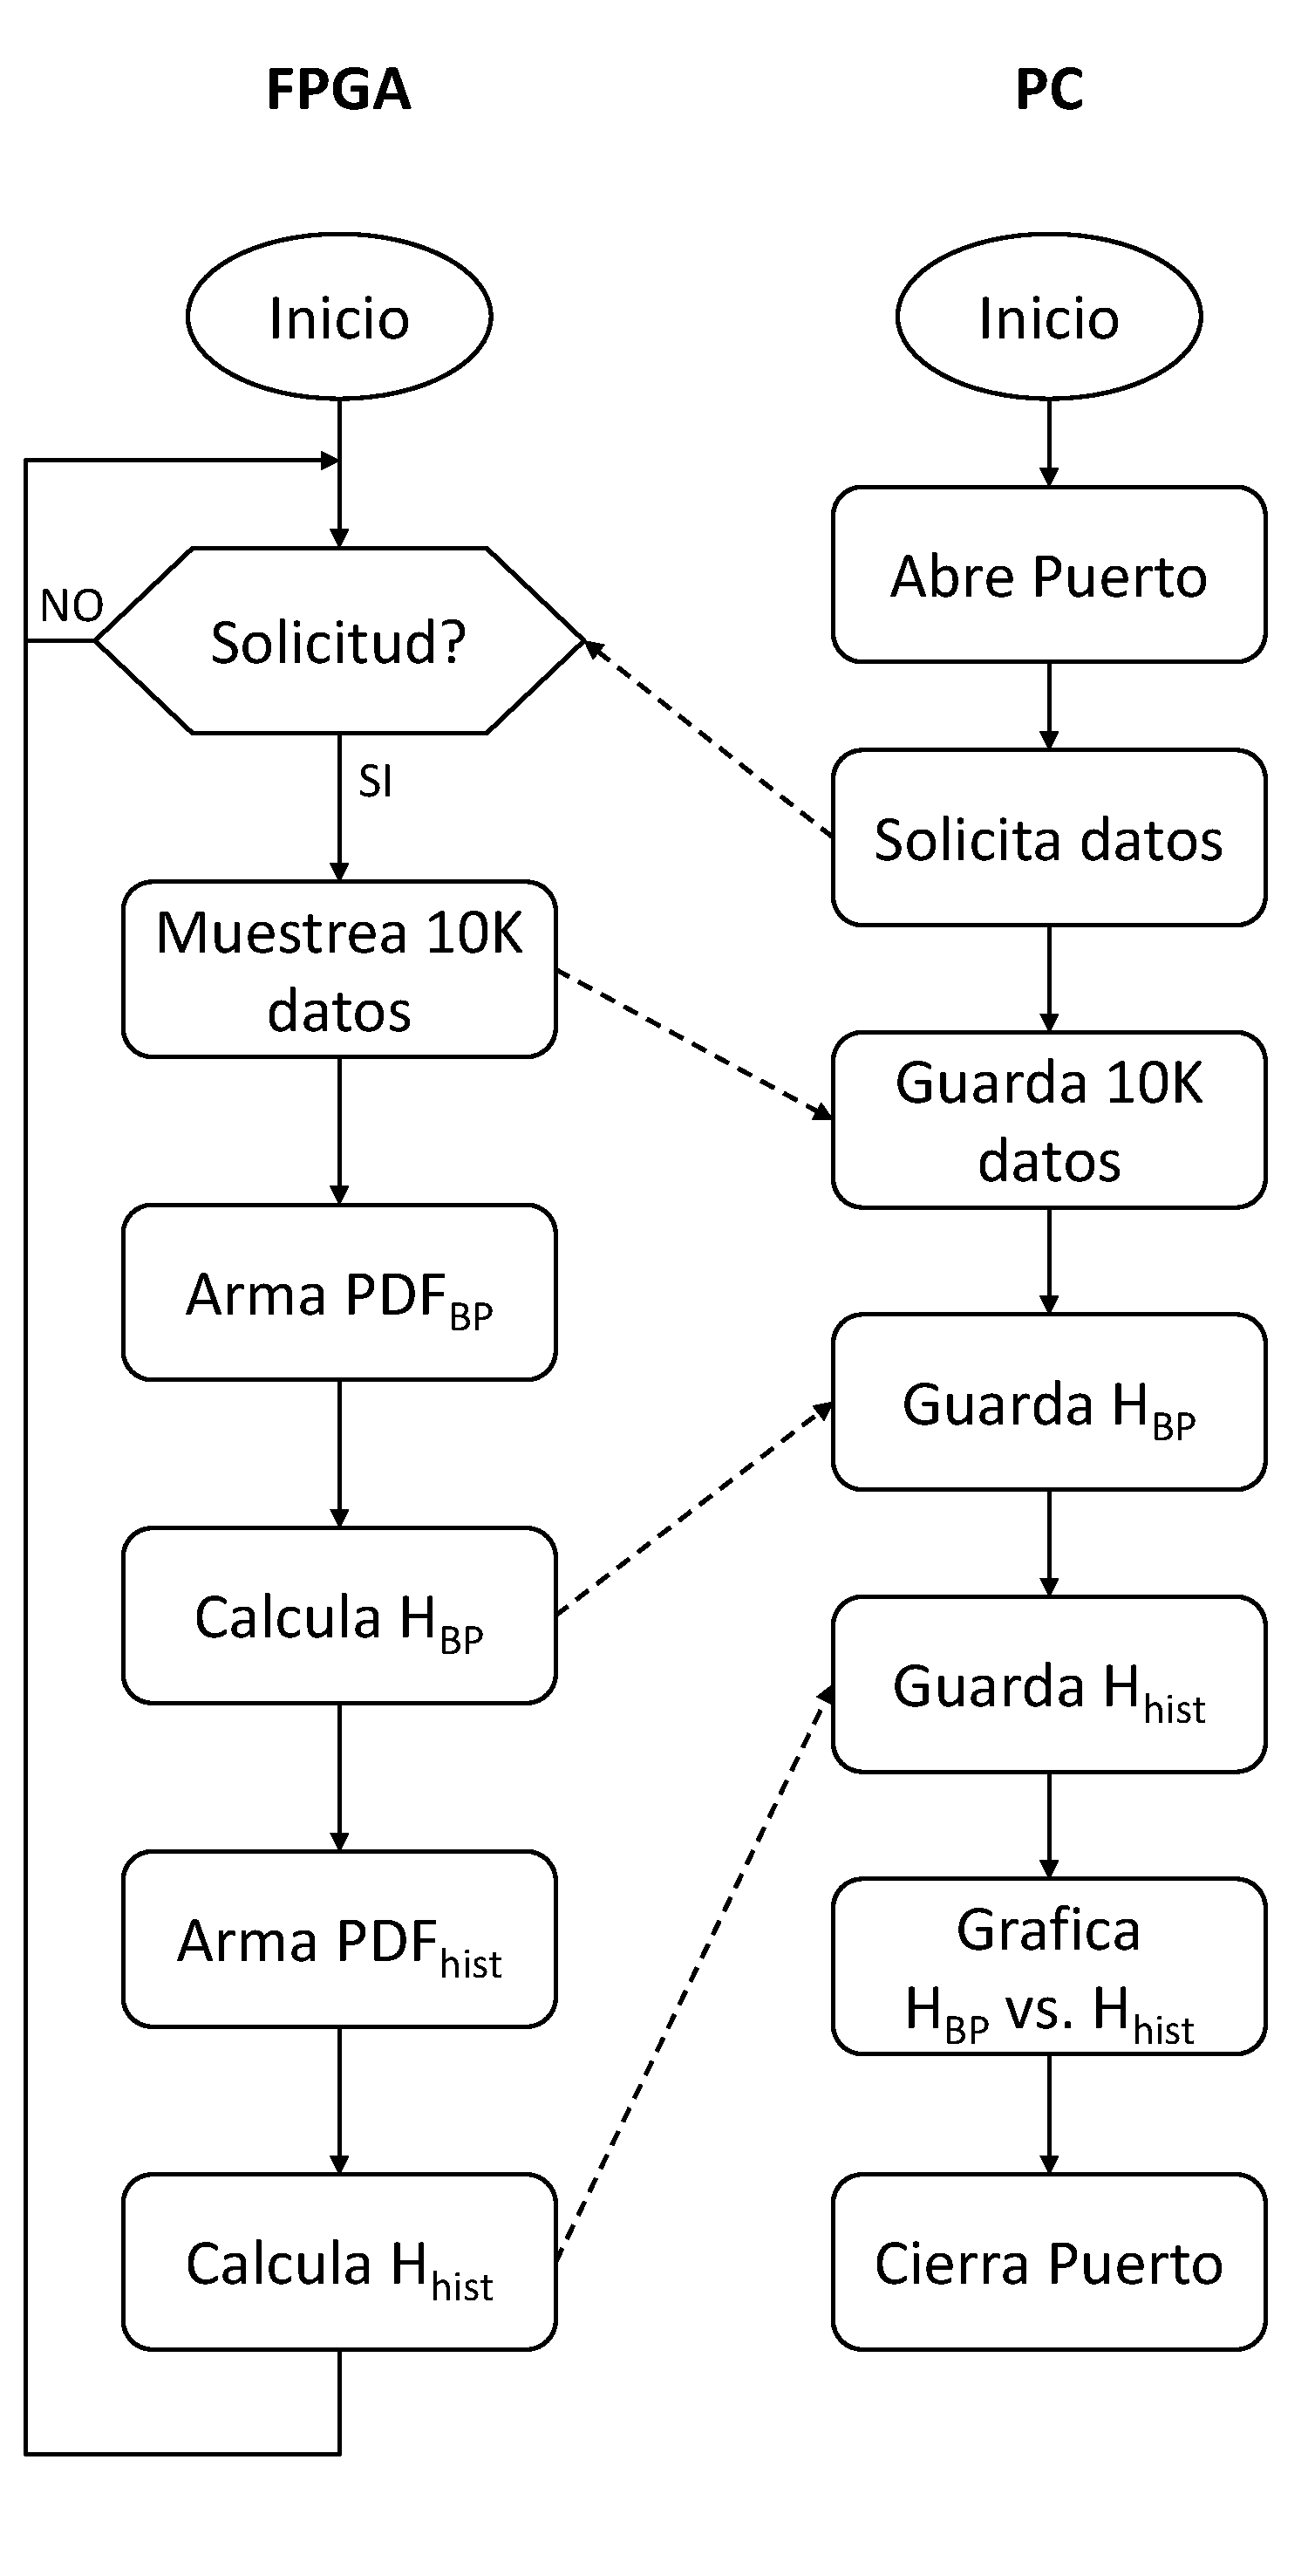
\includegraphics[width=0.7\columnwidth]{Soft}
	\caption{Diagrama de flujo del \textit{software} implementado.}\label{fig.softflow}
\end{figure}

En la PC corre un \textit{script} de Matlab que se encarga de abrir el puerto serie en donde se encuentra mapeado el USB, solicitar los datos, tomar los resultados del mismo puerto, graficarlos en un plano $H_{BP}$ vs. $H_{hist}$ y cerrar el puerto.

Sobre el microcontrolador en la FPGA corre un programa escrito en lenguaje C y compilado para el microcontrolador 8051 utilizando la herramienta \textit{SoftConsole~IDE~v3.4\textsuperscript\copyright}.
El firmware es una modificación del usado en \cite{Core8051sS}. Cuando se presenta una solicitud de datos por el puerto UART, se guardan los datos muestreados de la entrada analógica.
Luego, se recorre este vector generando las $PDF_{hist}$ y $PDF_{BP}$, a las que se les calcula sus respectivas entropías $H_{hist}$ y $H_{BP}$.
Estos resultados son enviados a la PC mediante el mismo puerto.

Con el fin de validar el sistema, el programa en la FPGA envía a  Matlab el vector de datos muestreados, para que se puedan calcular en la PC sus entropías y compararlas con los resultados del sistema implementado.

\subsubsection{Resultados}
\label{sec:resultados}

Como se dijo, para testear el sistema se compararon los resultados obtenidos por el sistema implementado y por un programa patrón que corre en la PC.
Para esto, se generaron $10~000$ muestras de señales con distintas formas de onda tanto externas (analógicas) como internas (digitales).

Las señales digitales fueron generadas por código en el microcontrolador, una corresponde a la función rand() de C y la otra al mapa caótico Logístico con parámetro r=4.

Las señales analógicas fueron generadas con el generador de funciones \textit{HP33120A}.
Tienen una amplitud de $4~Vpp$ y un nivel de continua de $2~V$ de forma de aprovechar todo el rango del conversor analógico-digital y aumentar la relación señal-ruido.
En los cuatro casos la frecuencia de las señales fue de $100~Hz$ y la velocidad de muestreo de $16~ks/s$.

El cuadro \ref{tablaErrores} muestra el error absoluto entre los resultados de los cuantificadores calculados en la FPGA comparados con los resultados calculados con el programa patrón sobre los mismos datos.
%
\begin{table}
	\centering
	\begin{tabular}{@{\extracolsep{\fill}}| c| c | c |c |}
		\hline
		\textbf{{Generador}} & \textbf{{Origen}} & \textbf{{Error}} \textbf{{$H_{BP}$}} & \textbf{\textbf{{Error}}} \textbf{{$H_{hist}$}} \\ \hline
		{Rand}               & {Digital}         & {$1,7421E^{-6}$}                     & {$2,6977E^{-6}$}                                \\ \hline
		{Logístico}          & {Digital}         & {$0,4256E^{-6}$}                     & {$94,693E^{-6}$}                                \\ \hline
		{Triangular}         & {Analógico}       & {$6,3445E^{-6}$}                     & {$2,0028EE^{-6}$}                               \\ \hline
		{Senoidal}           & {Analógico}       & {$6,3151E^{-6}$}                     & {$5,6506E^{-6}$}                                \\ \hline
		{Cuadrada}           & {Analógico}       & {$0,1797E^{-6}$}                     & {$1,9930EE^{-6}$}                               \\ \hline
		{Rampa}              & {Analógico}       & {$245,00E^{-6}$}                     & {$1,0876E^{-6}$}                                \\ \hline
	\end{tabular}
	\caption{Error de los cuantificadores evaluados en la FPGA con respecto a los resultados calculados por el programa patrón.}\label{tablaErrores}
\end{table}

La Figura \ref{fig:resultados} muestra los valores entregados por la FPGA en el plano $H_{BP}$ vs. $H_{hist}$.
%
\begin{figure}[htb]
	\centering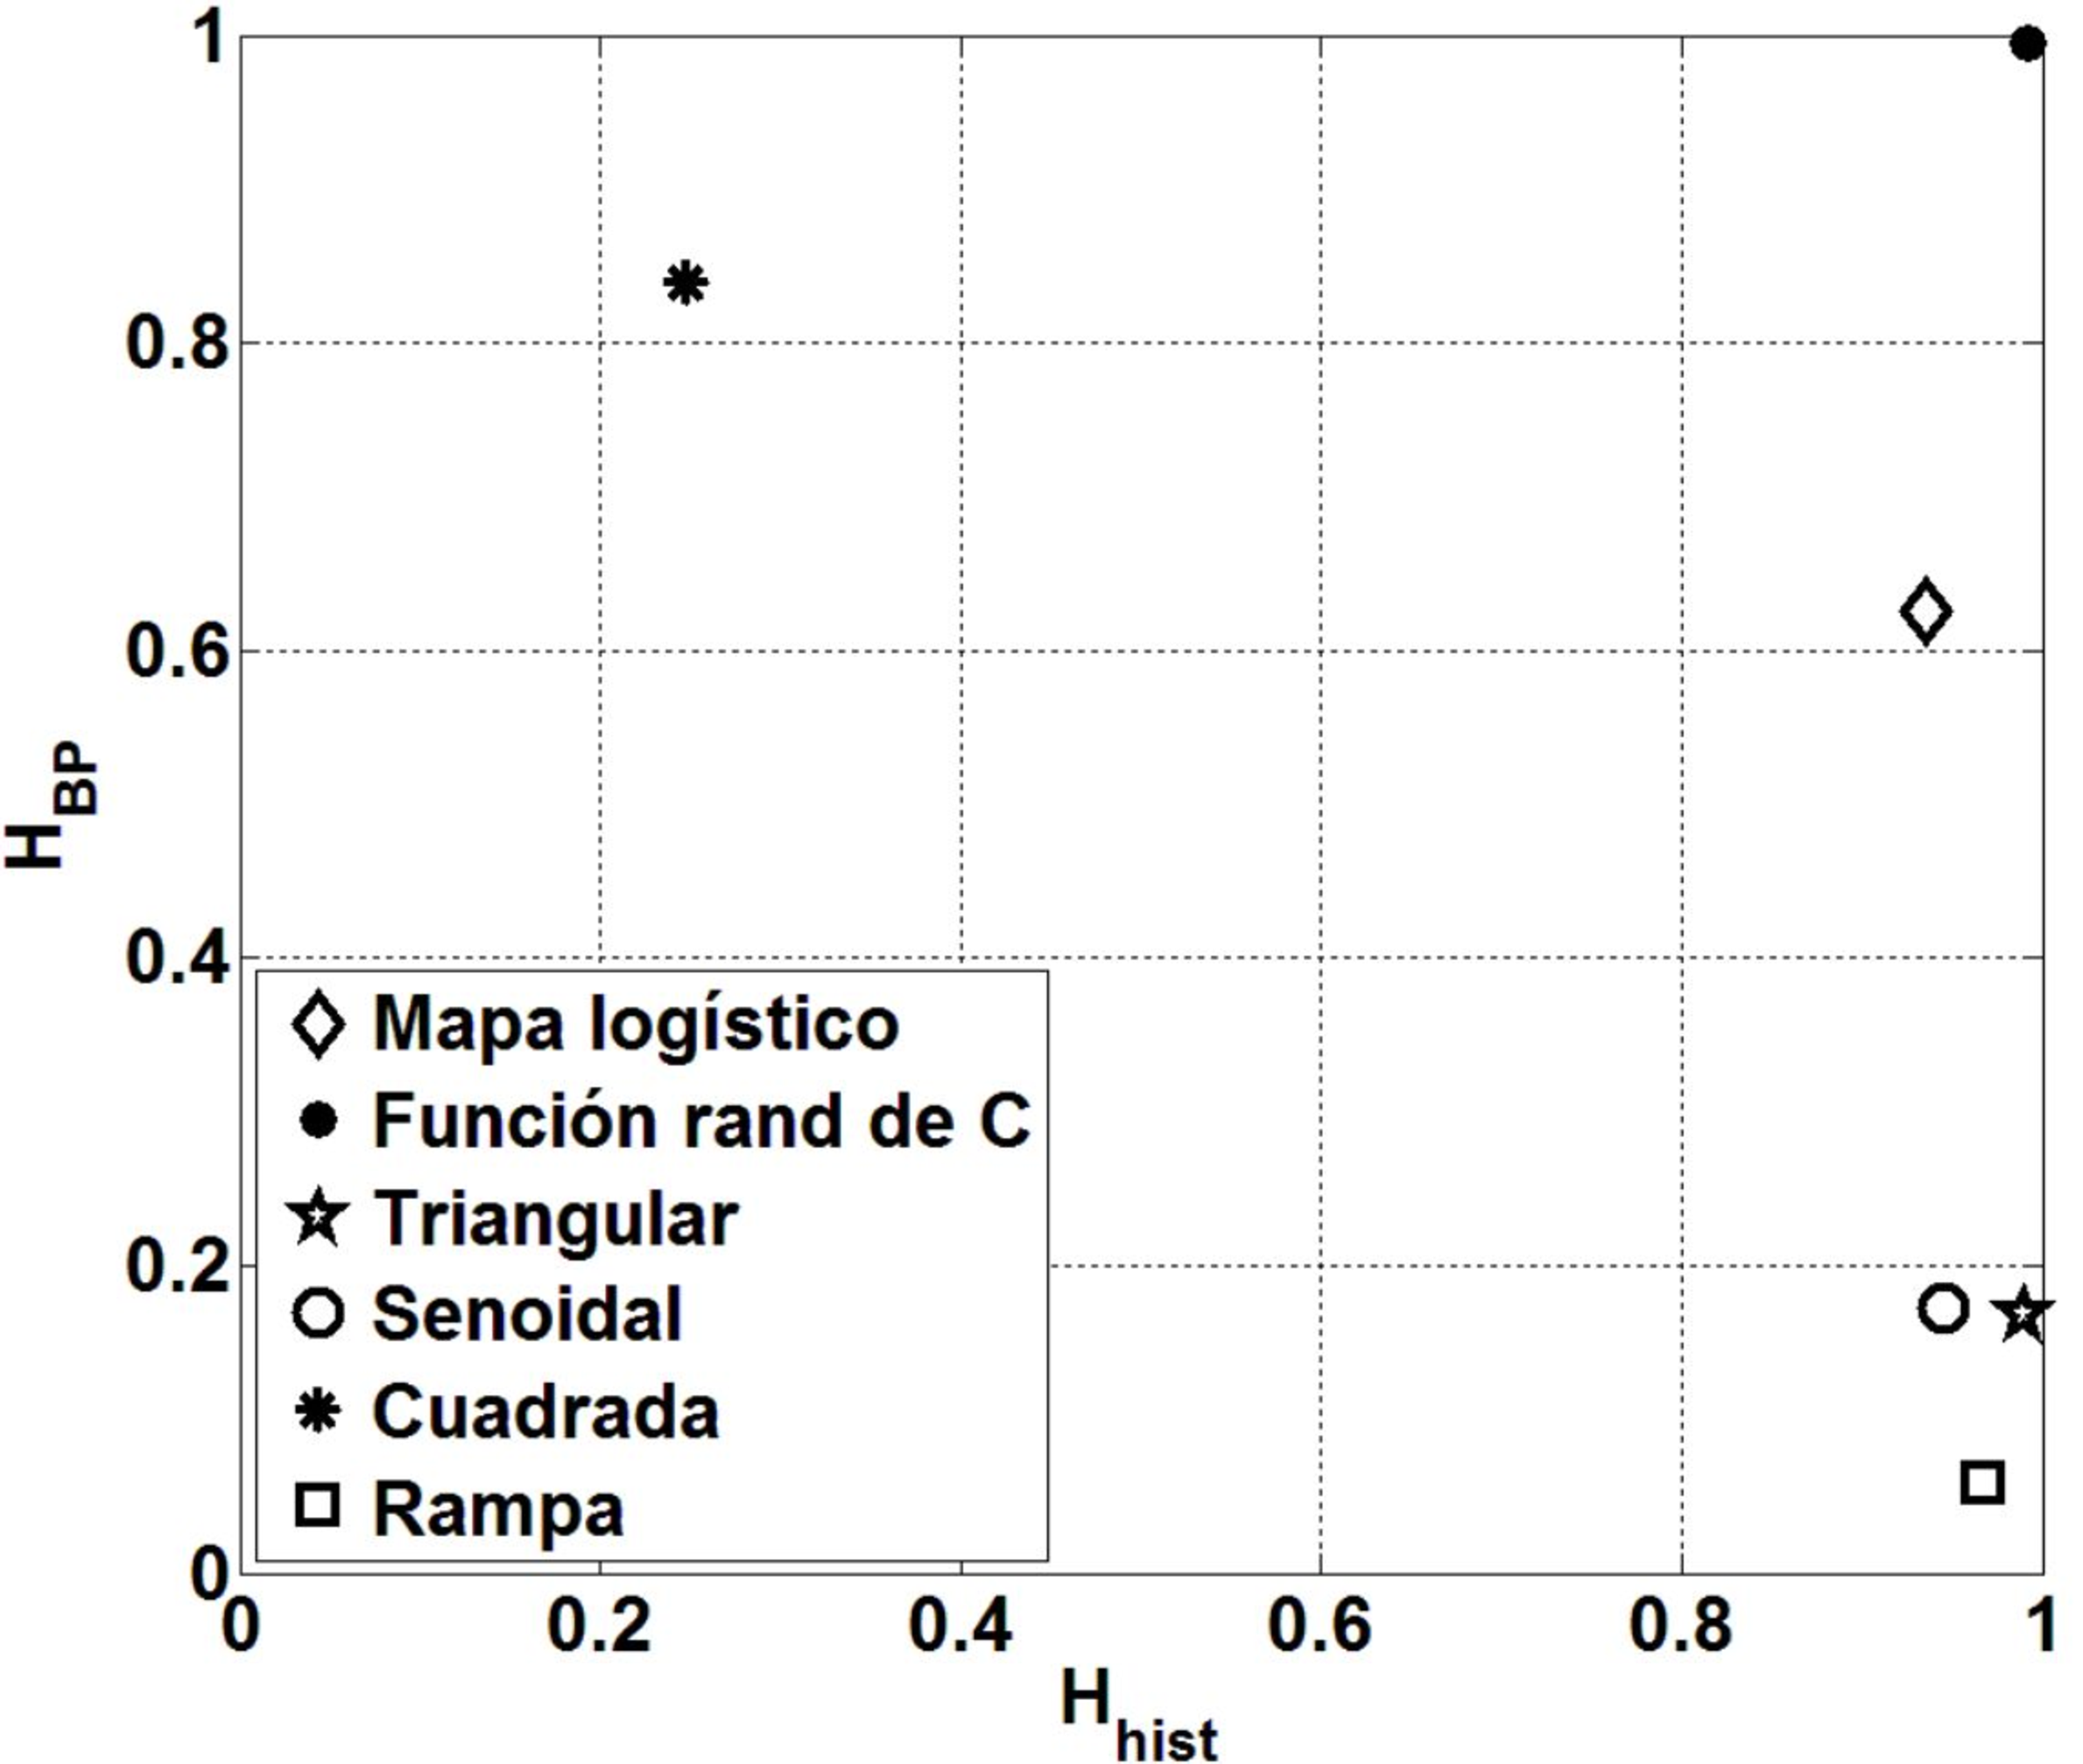
\includegraphics[width=.75\textwidth]{resultados}
	\caption{Resultados de las mediciones.}\label{fig:resultados}
\end{figure}

Los resultados de la compilación nos permiten conocer los recursos de la FPGA utilizados por el sistema completo y la cantidad de memoria ocupada por el \textit{software} que corre en el microcontrolador.
Recordemos que esta es una implementación de \textit{hardware} rígida, es decir primero se arma el circuito en la FPGA (microcontrolador, periféricos, etc.) y luego se carga el \textit{software} sobre él.

El reporte de la compilación de \textit{hardware} devuelto por el \textit{Place and Route} se muestra en la Figura \ref{fig:hard}. Podemos ver que la implementación utiliza un 19\% de los recursos lógicos de la FPGA, el $21\%$ de las celdas de entrada-salida y el $28\%$ de los bloques de memoria.
%
\begin{figure}[htb]
	\centering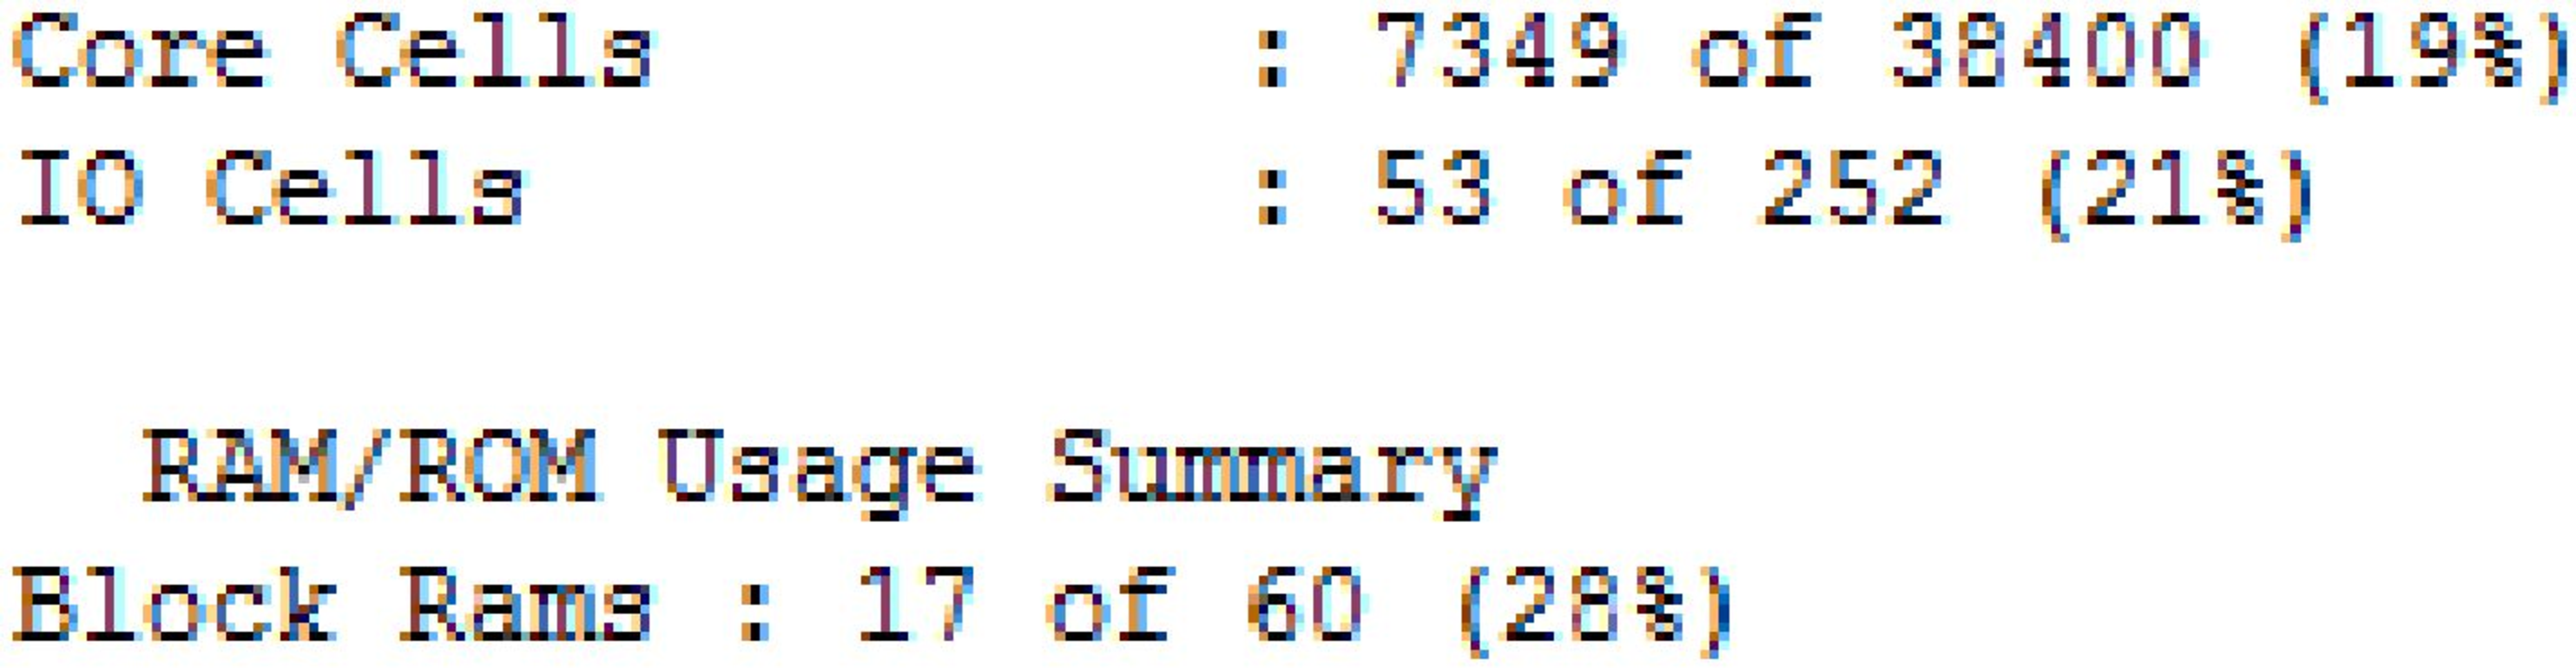
\includegraphics[scale=.13]{reporteHard}
	\caption{Recursos empleados por el \textit{hardware} del sistema.}\label{fig:hard}
\end{figure}

El reporte de la compilación de \textit{software} se muestra en la Figura \ref{fig:soft}.
Podemos ver que la memoria FLASH no volátil se encuentra ocupada al $15,4\%$.
Por otro lado, de las $47~145$ direcciones de memoria SRAM ocupada, $4~096$ son ocupadas por el bus APB y $43~049$ por las variables del programa.
%
\begin{figure}[htb]
	\centering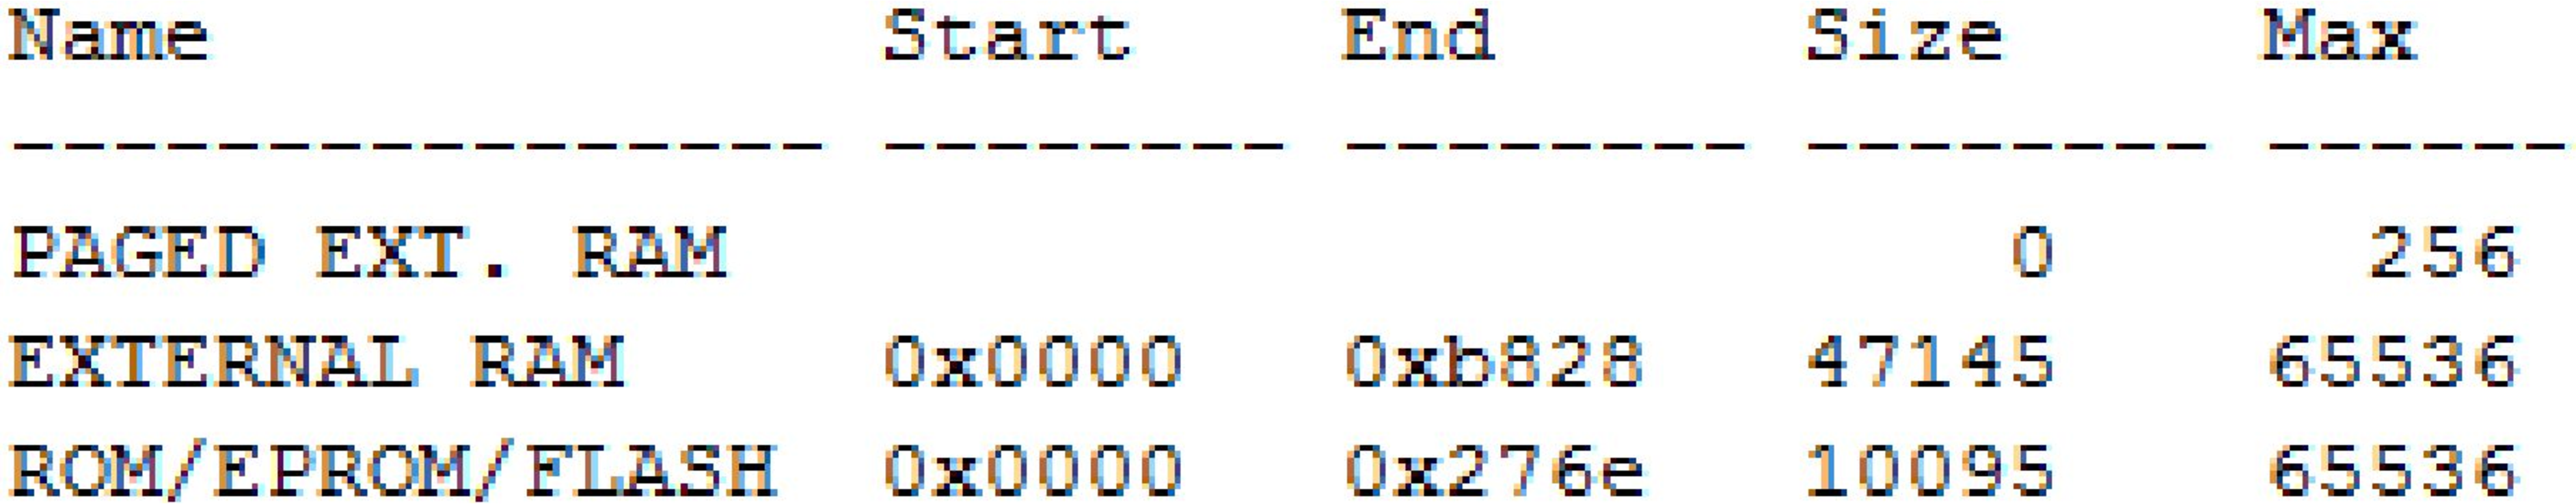
\includegraphics[scale=.13]{reporteSoft}
	\caption{Recursos empleados por el \textit{software} del sistema.}\label{fig:soft}
\end{figure}

El programa debió ser adaptado al microcontrolador instanciado en la FPGA.
Estas modificaciones hacen que la salida del sistema implementado no sea igual a la de un programa que corre en la PC, al cual tomamos como programa patrón.
Por esto se testeó el error cometido, para tener una cota y determinar si los resultados de los cuantificadores son correctos.
El programa patrón utiliza aritmética de $64~bits$ en punto flotante norma IEEE754-64~bits y emplea la librería math.h \cite{Mathe}.
Para el algoritmo en la FPGA se disminuyó la aritmética a 32 bits de punto flotante norma IEEE754-32~bits.
También se requirió el cálculo de la función logaritmo, que se implementó mediante un algoritmo de CORDIC.
En el Cuadro \ref{tablaErrores} se ve que el error absoluto no supera el sexto decimal, esto indica que se detecta diferencia recién a partir del quinto dígito decimal.

En la Figura \ref{fig:resultados} puede verse como los cuantificadores $H_{BP}$y $H_{hist}$ diferencian claramente las propiedades estadísticas de las series de datos analizadas.
Las señales Senoidal, Rampa y Triangular presentan un valor alto de $H_{hist}$ porque tienen casi todos los valores que es capaz de generar el conversor Analógico-Digital.
Sin embargo, la mezcla de estos datos es mala por tratarse de señales periódicas totalmente predecibles, esto se ve en el bajo valor de $H_{BP}$.
Un caso interesante de analizar es la señal Cuadrada.
El efecto del ruido aditivo es especialmente notable en las zonas en donde el valor de la señal debería ser constante.
Se generan dos Gaussianas muy finas en torno a los valores ideales en la $PDF_{hist}$, esto no afecta demasiado el valor calculado $H_{hist}$, sin embargo, para la $PDF_{BP}$, se calcula el patrón de orden directamente a la señal ruidosa, por lo que el valor de $H_{BP}$ es más alto que el esperado.
La señal generada mediante la función rand de C, presenta las mejores propiedades estadísticas ubicándose en el punto $\sim(1,1)$.
\subsection{Dinámica de los ITQ's con AWGN y Banda Limitada}
\label{ssec:TDdS}
	
En esta Sección exploramos la respuesta de un sistema de medición de entropías en presencia de ruido aditivo y señales filtradas.
Esta inquietud surge como resultado de la implementación detallada en la Sección \ref{ssecCuantiImpFPGA}.
El filtrado es inherente al ancho de banda del sistema de medición y las señales a medir siempre están contaminadas con ruido, por lo tanto es necesario caracterizar la respuesta de nuestro sistema de medición ante estos dos procesos.
Este trabajo es complementario al desarrollo de un sistema de medición de entropías implementado en FPGA.

\subsubsection{Filtrado digital}
\label{sec:filtrado}

Ya sea en la elección de un filtro como en cualquier problema de diseño en ingeniería, generalmente no es posible dar una respuesta posible acerca de cuál es al mejor solución. Se discute la posibilidad de la implementación de distintos filtros porque no hay un solo método de diseño ni un sólo tipo de filtro mejor para todas las circunstancias. La elección del tipo de filtro depende de la importancia de sus ventajas aplicadas a cada problema.

Un filtro ideal es aquel en el que la respuesta en frecuencia es unitaria en el rango de las frecuencias de paso, cero en la banda de rechazo y no posee banda de transición. Dada la inherente periodicidad de la respuesta en frecuencia para tiempo discreto esta tiene la apariencia de un tren rectangular en el dominio de las frecuencias, sin embargo en este trabajo sólo se muestra la frecuencia normalizada en el intervalo $(0,1)$. Entonces la transferencia de un filtro pasabajos ideal en frecuencia normalizada quedaría:
\begin{equation}
H_{LP}=
\left\{ 
\begin{aligned}
&1,\qquad|f-0,5|>f_c\\
&0,\qquad|f-0,5|<f_c
\end{aligned}
\right.
\end{equation}
Ecuación definida en el intervalo de frecuencias normalizadas $f\in\left(0,1\right)$.

El hecho de que no podemos contar con series de valores infinitamente largas para ser filtradas, equivale a decir que disponemos de una serie de muestras enventanada.
Como el producto en el dominio del tiempo equivale a una convolución en el dominio de la frecuencia, podemos estudiar el efecto que este enventanado tiene sobre la respuesta frecuencial del filtro.
Consideremos la ventana más sencilla; la ventana rectangular. Supongamos que la aplicamos sobre una versión retardada de la respuesta ideal, su efecto en el dominio de la frecuencia será la convolución entre la respuesta de nuestro filtro ideal y la transformada esta ventana rectangular, es decir una función $sinc$ de período $1/N$ en donde $N$ es la cantidad de muestras que entran en la ventana.

El efecto de enventanado o truncaminto de la respuesta es doble: por una parte, la anchura del lóbulo principal está relacionada con la aparición de una banda de transición en el filtro. Por otra, la presencia de lóbulos laterales (secundarios) lleva a la aparición de un ripple u oscilaciones en la respuesta en frecuencia, en ambas bandas, (más apreciable en la banda no pasante).
La aparición de los lóbulos secundarios se debe a que la ventana rectangular presenta una discontinuidad abrupta que, al pasar al dominio de la frecuencia, conlleva un reparto de la energía sobre todo el espectro a causa del aliasing.

Una opción que se plantea es generalizar el concepto de ventana y emplear ventanas más suaves que la rectangular para realizar el truncamiento de la respuesta deseada, esta técnica es una de las formas de realizar un filtro FIR.
Sin embargo, si analizamos la transformada de la ventana cuadrada vemos que presenta valores nulos cada $1/N$, que son los mismos lugares en donde aparecen las componentes espectrales de la DFT. Esto significa que los efectos de la ventana rectangular aparecen al convertir la respuesta de este filtro a tiempo continuo.

Otra opción sería diseñar un filtro analógico y transformar su respuesta a frecuencia discreta. Para esto existen fórmulas cerradas de diseño, por lo que es posible satisfacer casi cualquier especificación preestablecida. La utilización de esta técnica da como resultado un filtro IIR. Comparado con un filtro FIR, un filtro IIR requiere un orden mucho menor para cumplir las especificaciones de diseño.

En este caso se analizó la respuesta del sistema en el dominio digital.
Además, es necesario filtrar las componentes espectrales de a una, lo que requiere una banda de transición muy estrecha, esto reduce el conjunto de filtros posibles.
Por el lado del IIR se probó un filtro elíptico, este filtro presenta una banda de transición muy estrecha a costa de un ripple que aparece tanto en la banda de paso como en la de rechazo.
Por el lado del filtro FIR se utilizó un filtro ideal con una ventana rectangular que abarca toda la serie de valores.

\subsubsection{Resultados}

Para representar la dinámica en función del filtrado, se eligieron dos señales representativas (cuadrada y senoidal) y se les calcularon los cuantificadores descriptos en la Sección \ref{sec:ITQs} luego de ser filtrados por los filtros elegidos en la Sección anterior. Por otro lado, se calcularon los mismos cuantificadores a una señal de ruido blanco gaussiano.

En la Figura \ref{fig:flowchart} se muestra el procedimiento utilizado. Primero se generó un vector de ruido blanco gaussiano de $N=50~000$ muestras, la desviación estándar $\sigma$ es variable y se logra multiplicando al vector inicial de $\sigma=1$ por la desviación estándar elegida.
Luego se genera la señal determinística de $N=50~000$ muestras, período $T=100$ muestras y amplitud unitaria, que se sumó al ruido para lograr la señal contaminada.
La señal resultante se filtra para luego calcular cuantificadores.
Como se explicó más arriba, para calcular le entropía de valores se genera el histograma de valores y se lo normaliza para calcular la Función $PDF_{hist}$ a la que se le calcula la entropía de Shannon normalizada que da como resultado la entropía de valores normalizada $H_{hist}$.
Para calcular la entropía de patrones de orden se utilizó el histograma de patrones de orden que cuando se normaliza se consigue la función densidad de probabilidad de patrones de orden $PDF_{BP}$, a la que se le calcula la entropía de Shannon normalizada para conseguir la entropía de patrones de orden $H_{BP}$.
%
\begin{figure}[h]
\centering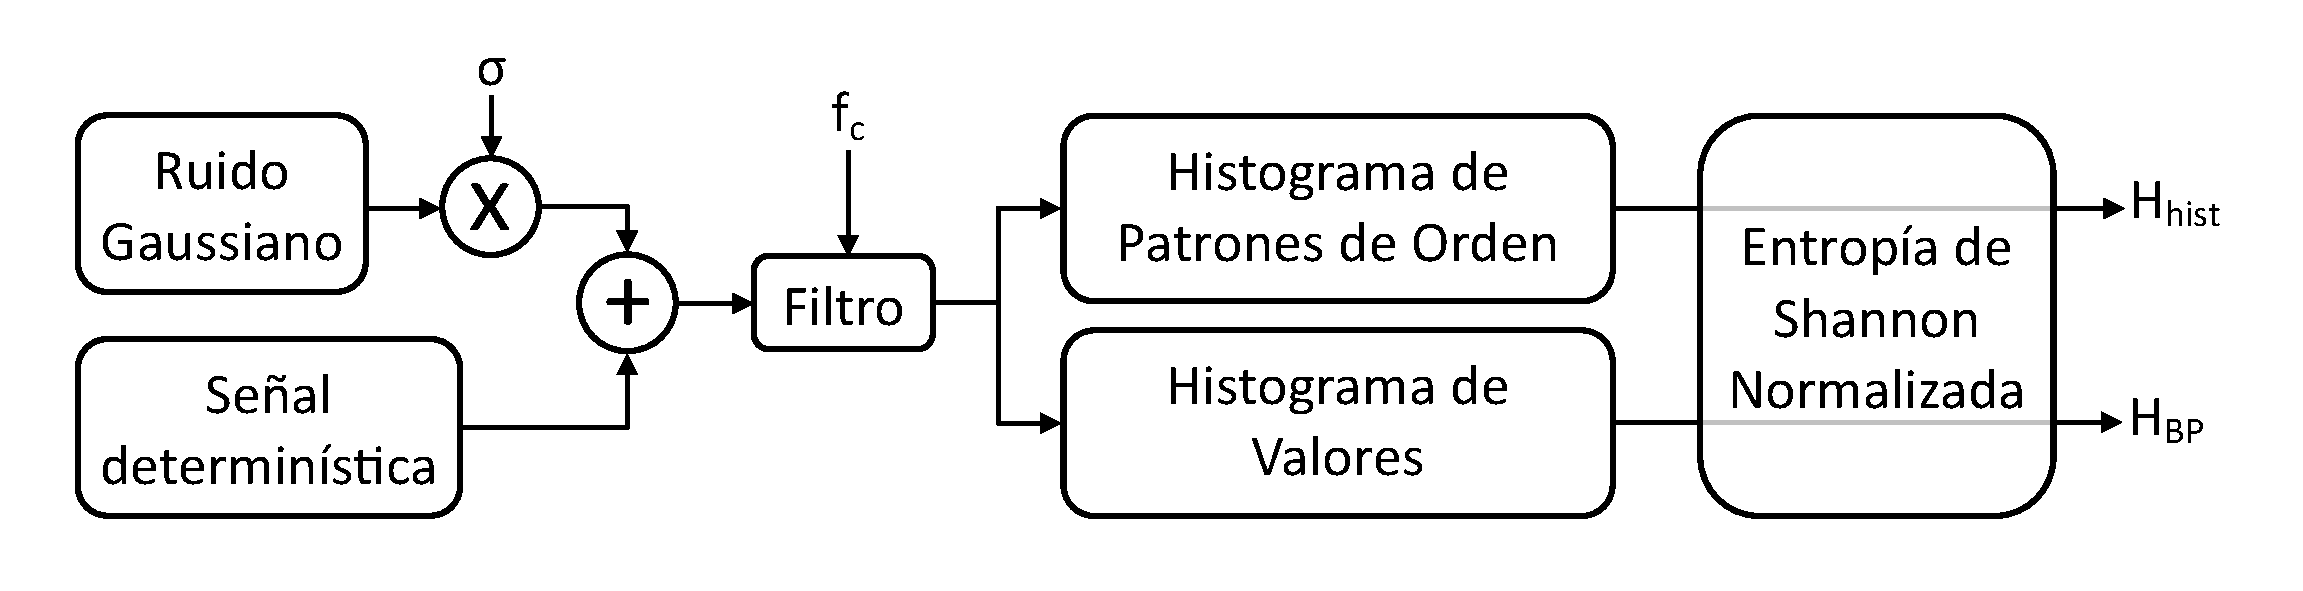
\includegraphics [width=0.99\textwidth]{FlowChart}
\caption {Diagrama de flujo del experimento.}\label{fig:flowchart}
\end{figure}

Para evaluar la contribución de cada componente espectral a las entropías, se evaluaron dos filtros.
Primero se aplicó un filtro elíptico de orden $10$ con ripple pasabanda de $0,5 dB$, ripple en la banda de rechazo de $100 dB$ y frecuencia de corte variable $f_c$, en la Figura \ref{fig:filtroellip} se muestra su respuesta en ganancia (Figura \ref{subfig:filtroellip_amplitud}) y fase (Figura \ref{subfig:filtroellip_frecuencia}) para el caso de $f_c=0,5$. De esta forma se logra un filtrado lo suficientemente abrupto como para considerar que a medida que se barren distintas frecuencias de corte se eliminan componentes espectrales individualmente.
Los resultados de este filtrado se compararon con los resultados de un filtro ideal (Figura \ref{fig:filtroideal}), que consiste en una máscara aplicada a la transformada de fourier de la señal a filtrar, de esta manera se consigue el espectro de la señal filtrada, el cual es antitransformado para recuperar la versión filtrada en las muestras. El diagrama de este filtro puede verse en la Figura \ref{subfig:filtroideal_diagrama}. Este procedimiento equivale a un filtrado ideal sin retardo, por lo que el bode de amplitud es $0dB$ en la banda de paso y $-\infty dB$ en la banda de rechazo (Figura \ref{subfig:filtroideal_diagrama}); la fase $\omega\tau=0$ es lineal con pendiente nula (Figura \ref{subfig:filtroideal_frecuencia}).
%
\begin{figure}[h]
    \centering
    \begin{subfigure}[t]{.49\textwidth}
        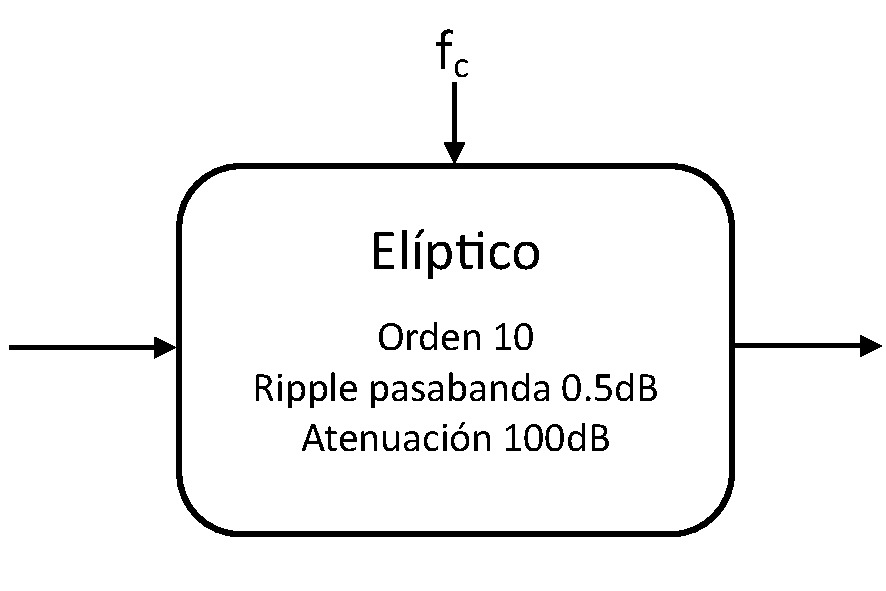
\includegraphics[width=\textwidth]{Ellip}
        \caption{Esquema}
        \label{subfig:filtroellip_diagrama}
    \end{subfigure}
    ~ %add desired spacing between images, e. g. ~, \quad, \qquad, \hfill etc. 
      %(or a blank line to force the subfigure onto a new line)
    \begin{subfigure}[t]{.49\textwidth}
        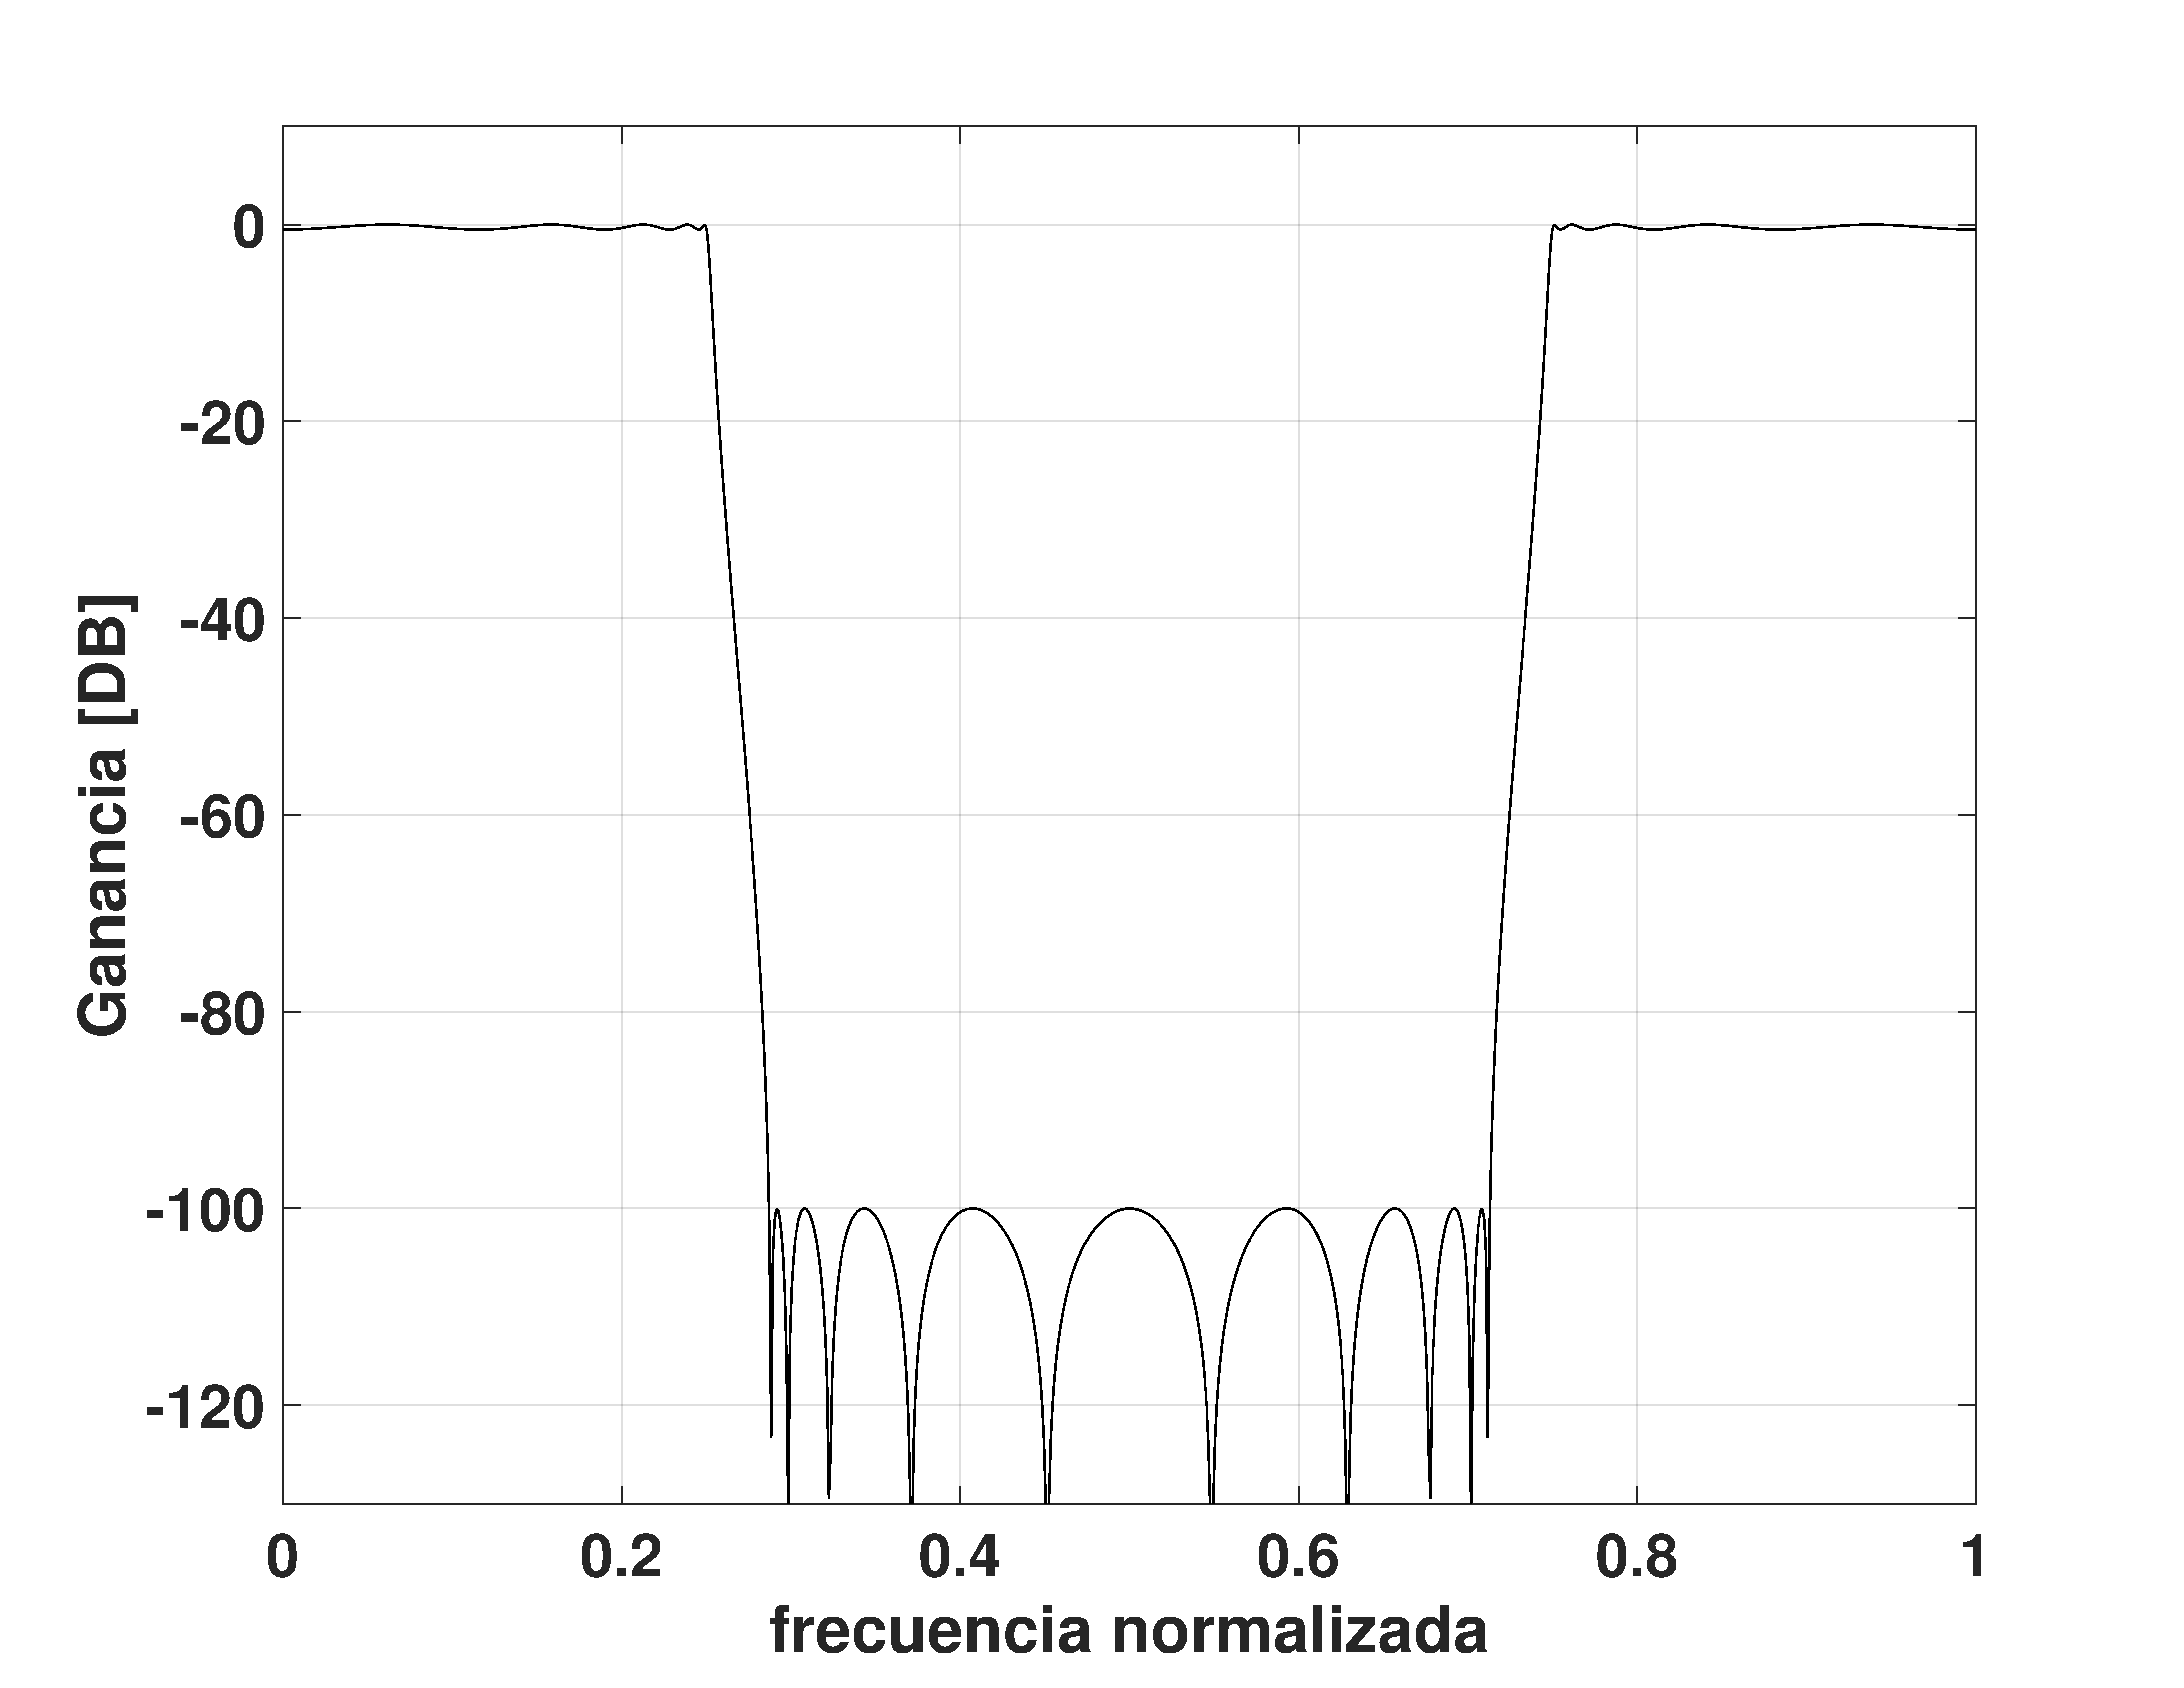
\includegraphics[width=\textwidth]{BodeEllip}
        \caption{Bode de ganancia}
        \label{subfig:filtroellip_amplitud}
    \end{subfigure}
    ~ %add desired spacing between images, e. g. ~, \quad, \qquad, \hfill etc. 
    %(or a blank line to force the subfigure onto a new line)
    \begin{subfigure}[t]{.49\textwidth}
        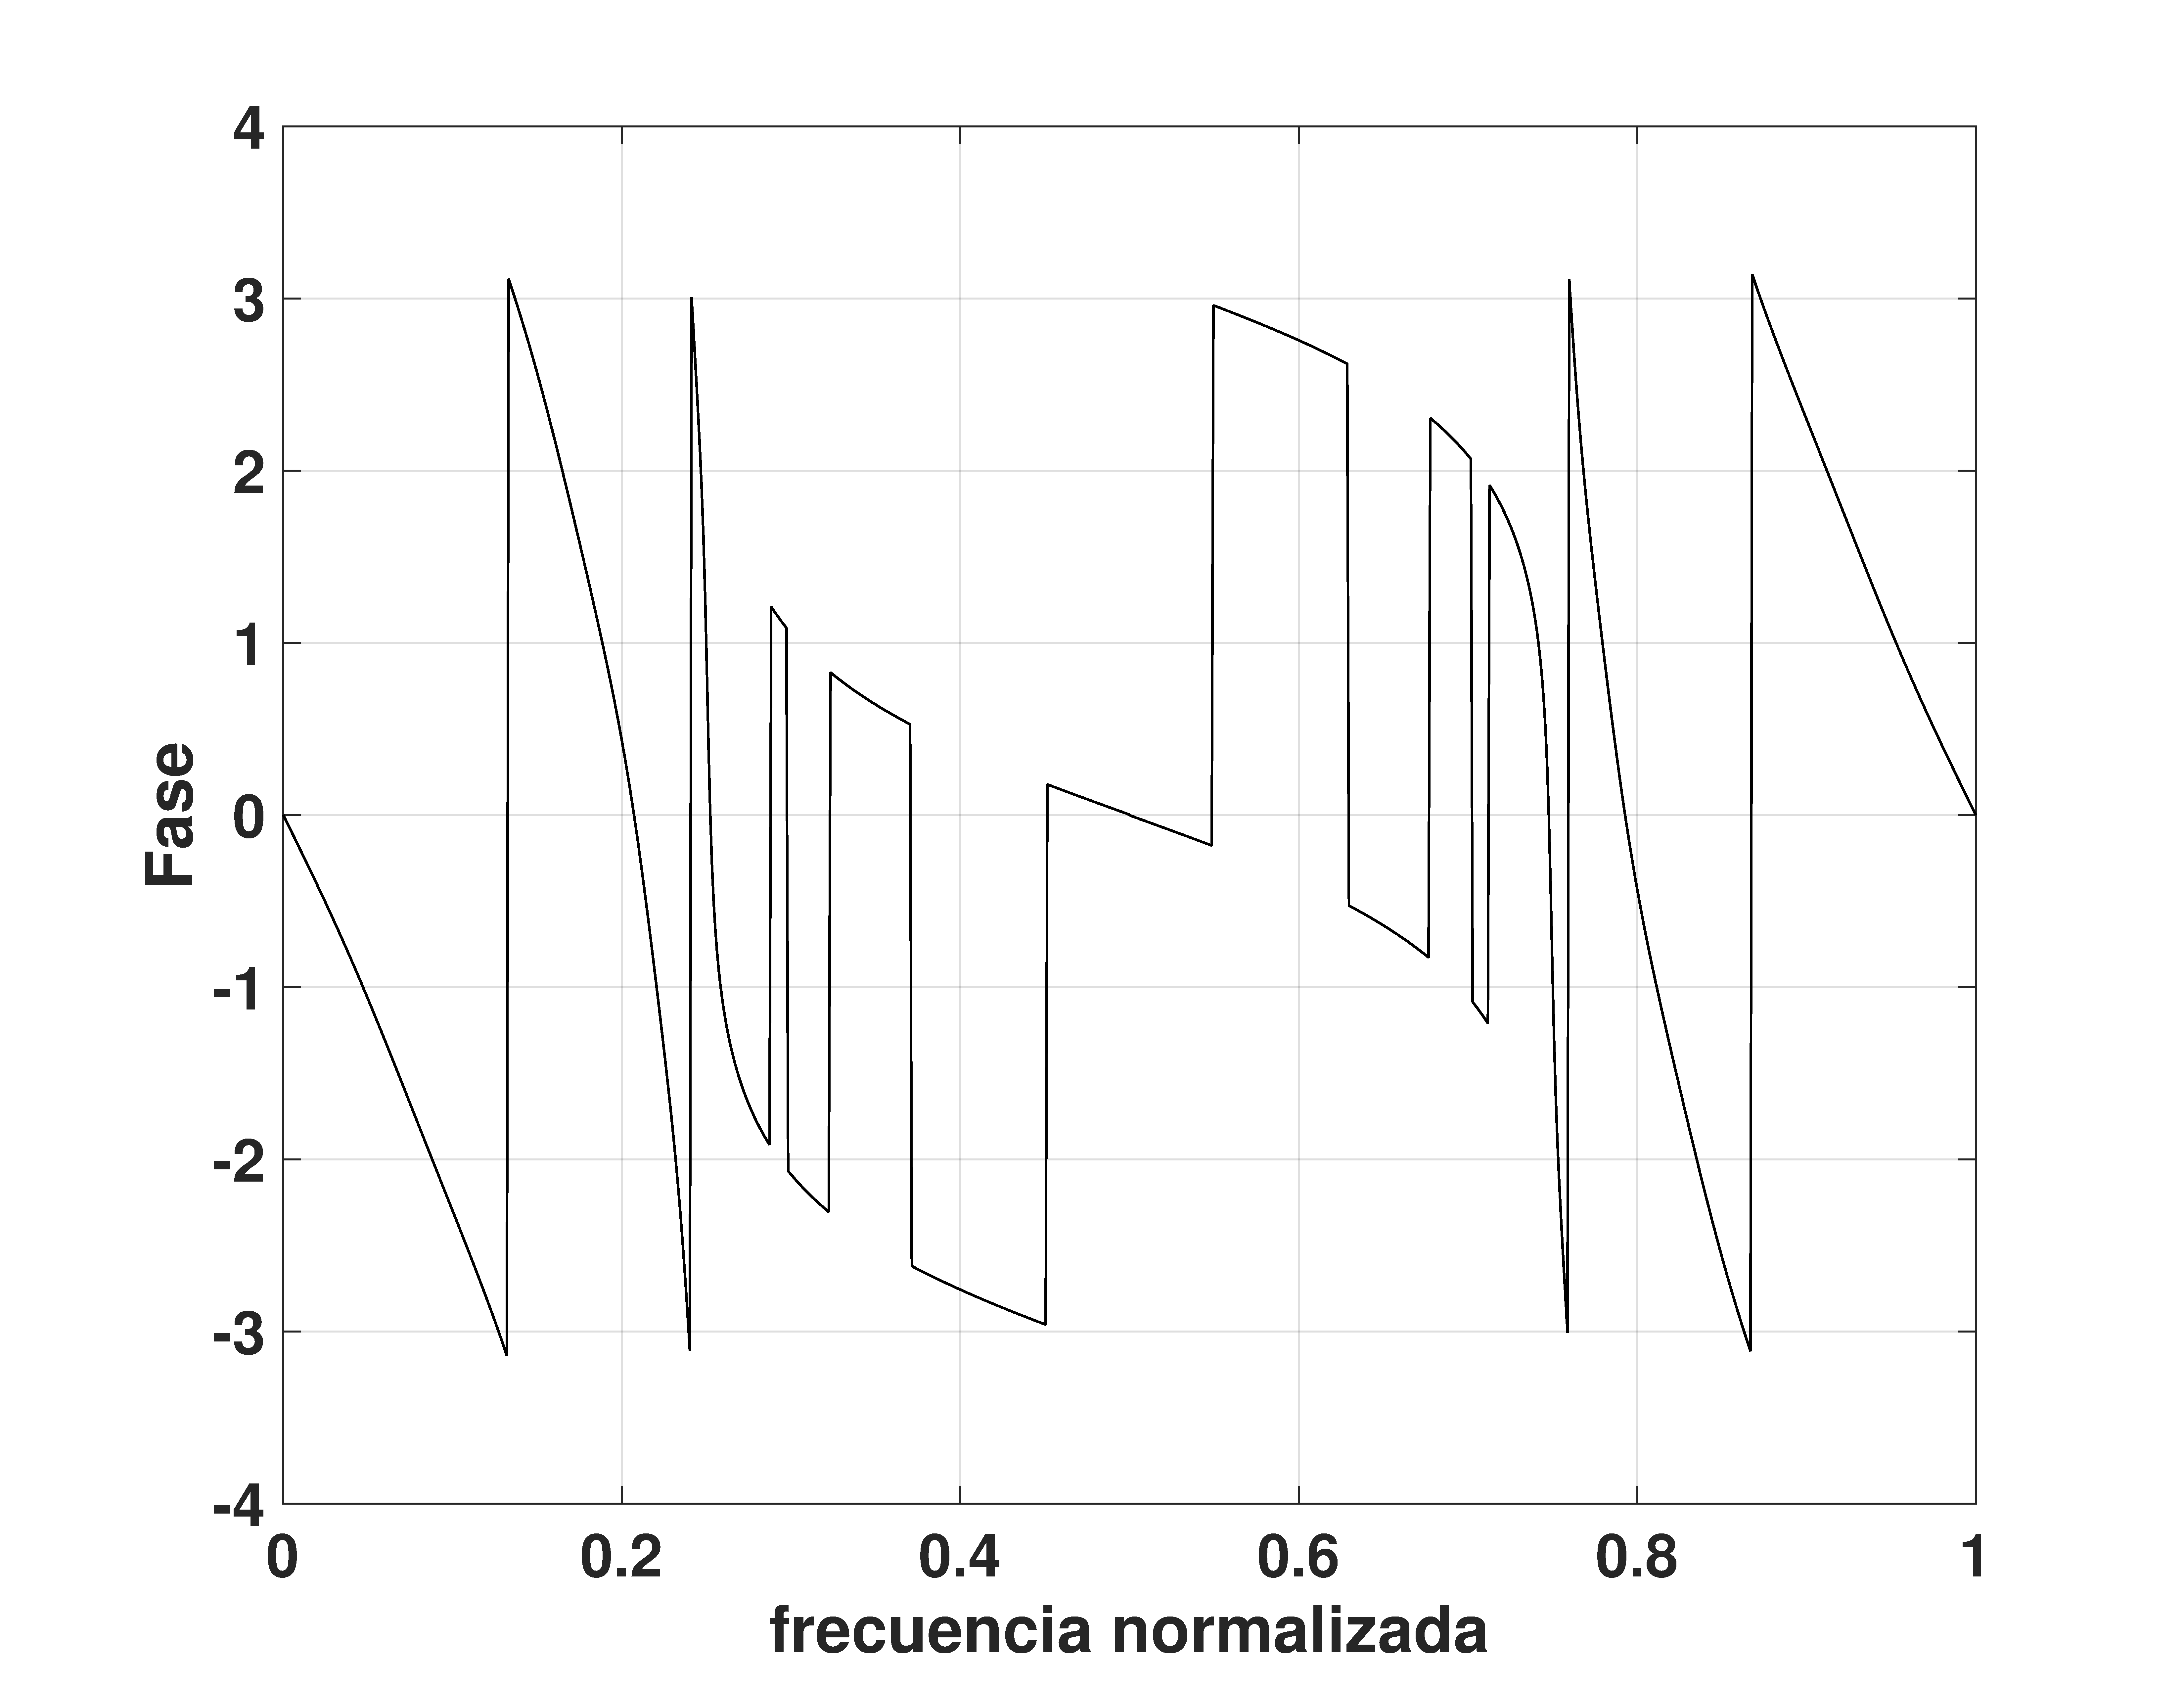
\includegraphics[width=\textwidth]{FreqEllip}
        \caption{Bode de fase}
        \label{subfig:filtroellip_frecuencia}
    \end{subfigure}
    \caption{Filtro elíptico.}\label{fig:filtroellip}
\end{figure}
%
\begin{figure}[h]
    \centering
    \begin{subfigure}[t]{.49\textwidth}
        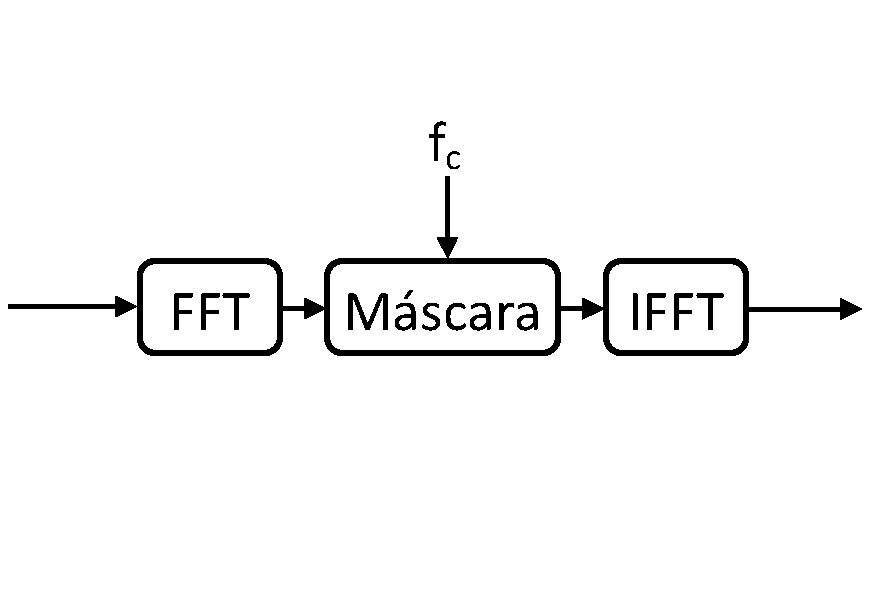
\includegraphics[width=\textwidth]{Ideal}
        \caption{Esquema}
        \label{subfig:filtroideal_diagrama}
    \end{subfigure}
    ~ %add desired spacing between images, e. g. ~, \quad, \qquad, \hfill etc. 
      %(or a blank line to force the subfigure onto a new line)
    \begin{subfigure}[t]{.49\textwidth}
        \includegraphics[width=\textwidth]{BodeIdeal}
        \caption{Bode de ganancia}
        \label{subfig:filtroideal_amplitud}
    \end{subfigure}
    ~ %add desired spacing between images, e. g. ~, \quad, \qquad, \hfill etc. 
    %(or a blank line to force the subfigure onto a new line)
    \begin{subfigure}[t]{.49\textwidth}
        \includegraphics[width=\textwidth]{FreqIdeal}
        \caption{Bode de fase}
        \label{subfig:filtroideal_frecuencia}
    \end{subfigure}
    \caption{Filtro ideal.}\label{fig:filtroideal}
\end{figure}

Primero se aplicó una señal de ruido blanco gaussiano, es decir que la señal determinística es cero y la desviación estándar de la gaussiana unitaria.
En la Figura \ref{fig:ellip} se muestra el resultado de los cuantificadores a medida que se va barriendo la frecuencia de corte del filtro elíptico.
En la Figura \ref{subfig:ellip_Hhist} se muestra la entropía del histograma de valores $H_{hist}$, puede verse que su valor se mantiene constante alrededor de $0,9$ tanto para el filtro pasa-bajos (roja) como el pasa-altos (azul), este valor es el mismo que resulta de calcular la entropía del histograma de valores a la señal sin filtrar (resultado que se muestra con una línea punteada negra en el mismo gráfico). También puede verse que cuando la frecuencia de corte del filtro elíptico se acerca a los extremos el valor del cuantificador cae, en estas frecuencias el método numérico que calcula el vector filtrado diverge debido a la precisión finita.
En la Figura \ref{subfig:ellip_Hbp} se muestra la entropía de los patrones de orden, $H_{BP}$ se mantiene en valores bajos cuando el filtro (pasa-altos en azul y pasa-bajos en rojo) deja pasar pocas componentes espectrales. Luego, a medida que la frecuencia de corte deja pasar más componentes espectrales, el cuantificador tiende a $1$, que es justamente el valor que arroja cuando se ingresa con la señal sin filtrar (este valor está indicado con una línea punteada negra).
El cuantificador detecta los cambios en la forma de la señal a medida que es filtrada.
Por último, en el plano $H_{hist} - H_{BP}$ de la Figura \ref{subfig:ellip_HbpHhist} se compacta la información de ambos cuantificadores, aunque se pierde la noción de la frecuencia de corte.
%
\begin{figure}[h]
    \centering
    \begin{subfigure}[t]{.49\textwidth}
        \includegraphics[width=\textwidth]{RuidoEllip_Hhist}
        \caption{Entropía de valores normalizada}
        \label{subfig:ellip_Hhist}
    \end{subfigure}
    ~ %add desired spacing between images, e. g. ~, \quad, \qquad, \hfill etc. 
      %(or a blank line to force the subfigure onto a new line)
    \begin{subfigure}[t]{.49\textwidth}
        \includegraphics[width=\textwidth]{RuidoEllip_Hbp}
        \caption{Entropía de patrones de orden normalizada}
        \label{subfig:ellip_Hbp}
    \end{subfigure}
    ~ %add desired spacing between images, e. g. ~, \quad, \qquad, \hfill etc. 
    %(or a blank line to force the subfigure onto a new line)
    \begin{subfigure}[t]{.49\textwidth}
        \includegraphics[width=\textwidth]{RuidoEllip_Hbp_Hhist}
        \caption{Plano doble entropía}
        \label{subfig:ellip_HbpHhist}
    \end{subfigure}
    \caption{Cuantificadores calculados sobre la salida del filtro elíptico cuando se ingresa con ruido blanco gaussiano.}\label{fig:ellip}
\end{figure}

En la Figura \ref{fig:ideal} se muestran los resultados del mismo procedimiento pero cuando se aplica un filtro ideal.
El comportamiento de los cuantificadores es igual al del filtro elíptico en todos los casos con la diferencia que el método no diverge cuando $f_c\to1$ o $f_c\to0$.
Pueden verse por lo tanto los valores que arrojan los cuantificadores en los extremos de la frecuencia de corte.
La entropía no causal de la Figura \ref{subfig:ideal_Hhist} aumenta levemente en los extremos, en donde el histograma de valores deja de tener una distribución gaussiana y se aplana levemente.
También puede verse en la Figura \ref{subfig:ideal_Hbp} que la entropía de valores $H_{BP}\to0,15$ cuando $f_c\to0$ para el pasa-bajos (rojo) y para el pasa-altos (azul) $H_{BP}\to0,22$ cuando $f_c\to1$.
En este caso es fácil comparar la sensibilidad al filtrado de ambos cuantificadores, en el plano doble entropía de la Figura \ref{subfig:ideal_HbpHhist}.
El círculo blanco muestra la posición en este plano cuando ningún filtro es aplicado, podemos ver que el apartamiento en el eje vertical aumenta a medida que la serie es filtrada, mientras que no se aparta en el sentido horizontal.
Esto muestra que la sensibilidad al filtrado de $H_{BP}$ es mucho mayor que la de $H_{hist}$.
%
\begin{figure}[h]
    \centering
    \begin{subfigure}[t]{.49\textwidth}
        \includegraphics[width=\textwidth]{Ruido_Hhist}
        \caption{Entropía de valores normalizada}
        \label{subfig:ideal_Hhist}
    \end{subfigure}
    ~ %add desired spacing between images, e. g. ~, \quad, \qquad, \hfill etc. 
      %(or a blank line to force the subfigure onto a new line)
    \begin{subfigure}[t]{.49\textwidth}
        \includegraphics[width=\textwidth]{Ruido_Hbp}
        \caption{Entropía de patrones de orden normalizada}
        \label{subfig:ideal_Hbp}
    \end{subfigure}
    ~ %add desired spacing between images, e. g. ~, \quad, \qquad, \hfill etc. 
    %(or a blank line to force the subfigure onto a new line)
    \begin{subfigure}[t]{.49\textwidth}
        \includegraphics[width=\textwidth]{Ruido_Hbp_Hhist}
        \caption{Plano doble entropía}
        \label{subfig:ideal_HbpHhist}
    \end{subfigure}
    \caption{Cuantificadores calculados sobre la salida del filtro ideal cuando se ingresa con ruido blanco gaussiano.}\label{fig:ideal}
\end{figure}

Para el sistema planteado no se necesita volver al dominio continuo analógico, por lo que las dificultades mencionadas en la Sección \ref{sec:filtrado} respecto al filtrado ideal (como ripple en las bandas de paso y rechazo) no aplican a este caso.
Por este motivo para esta serie de pruebas elegimos el filtro ideal, dado que presenta mejores resultados que el elíptico.

La primer señal determinística que se muestra es una senoidal de amplitud unitaria con $100$ muestras por período, los resultados pueden verse en la Figura \ref{fig:Senoidal}.
Mientras la única componente espectral no es filtrada, el valor de la entropía de valores es $H_{hist}\approx0,57$ en la Figura \ref{subfig:Senoidal_Hhist} y la entropía de patrones de orden $H_{BP}\approx0,16$ en la Figura \ref{subfig:Senoidal_Hbp}.
Ambos cuantificadores caen a cero cuando la única componente espectral es filtrada, ya sea por el filtro pasa-bajos (azul) o por el pasa-altos (rojo).
El plano doble entropía muestra un punto en $\left(0,57;0,16\right)$ para la senoidal sin filtrar y otro en $\left(0;0\right)$ cuando la única componente espectral es filtrada.
%
\begin{figure}[h]
    \centering
    \begin{subfigure}[t]{.49\textwidth}
        \includegraphics[width=\textwidth]{Senoidal_Hhist}
        \caption{Entropía de valores normalizada}
        \label{subfig:Senoidal_Hhist}
    \end{subfigure}
    ~ %add desired spacing between images, e. g. ~, \quad, \qquad, \hfill etc. 
      %(or a blank line to force the subfigure onto a new line)
    \begin{subfigure}[t]{.49\textwidth}
        \includegraphics[width=\textwidth]{Senoidal_Hbp}
        \caption{Entropía de patrones de orden normalizada}
        \label{subfig:Senoidal_Hbp}
    \end{subfigure}
    ~ %add desired spacing between images, e. g. ~, \quad, \qquad, \hfill etc. 
    %(or a blank line to force the subfigure onto a new line)
    \begin{subfigure}[t]{.49\textwidth}
        \includegraphics[width=\textwidth]{Senoidal_Hbp_Hhist}
        \caption{Plano doble entropía}
        \label{subfig:Senoidal_HbpHhist}
    \end{subfigure}
    \caption{Cuantificadores calculados sobre la salida del filtro ideal cuando se ingresa con una señal senoidal limpia.}\label{fig:Senoidal}
\end{figure}

La salida de los cuantificadores cuando esta señal es contaminada con ruido gaussiano aditivo con $\sigma=0,2$ puede verse en la Figura \ref{fig:SenoidalRuidosa}.
Vemos en la Figura \ref{subfig:SenoidalRuidosa_Hhist} que la entropía de valores aumenta cuando el filtrado no elimina la componente espectral, dando valores incluso por encima del valor de la entropía de la señal gaussiana.
Esto se debe a que la PDF de amplitudes de la señal senoidal es complementaria con la de la señal gaussiana, entonces la PDF de amplitudes de la resultante es más parecida a la del ruido uniforme.
Para los patrones de orden de la Figura \ref{subfig:SenoidalRuidosa_Hbp}, el filtro pasa-altos no deja ver un cambio significativo debido a que la componente espectral de la senoidal es eliminada en la zona en la que su entropía es alta.
El filtro pasa-bajos en cambio muestra que mientras esta componente está presente el valor de la entropía es asintótico a el valor $H_{BP}\to0,16$ a medida que la frecuencia de corte disminuye.
Recordemos que $H_{BP}\approx0,16$ es el valor de la entropía de patrones de orden de la señal senoidal limpia.
En el plano doble entropía (Figura \ref{subfig:SenoidalRuidosa_HbpHhist}) se ve que ambos cuantificadores son complementarios, en el sentido que la entropía de valores detecta la presencia o no de la señal determinística mientras que la entropía de patrones de orden detecta el efecto del filtrado sobre la señal de ruido.
%
\begin{figure}[h]
    \centering
    \begin{subfigure}[t]{.49\textwidth}
        \includegraphics[width=\textwidth]{SenoidalRuidosa_Hhist}
        \caption{Entropía de valores normalizada}
        \label{subfig:SenoidalRuidosa_Hhist}
    \end{subfigure}
    ~ %add desired spacing between images, e. g. ~, \quad, \qquad, \hfill etc. 
      %(or a blank line to force the subfigure onto a new line)
    \begin{subfigure}[t]{.49\textwidth}
        \includegraphics[width=\textwidth]{SenoidalRuidosa_Hbp}
        \caption{Entropía de patrones de orden normalizada}
        \label{subfig:SenoidalRuidosa_Hbp}
    \end{subfigure}
    ~ %add desired spacing between images, e. g. ~, \quad, \qquad, \hfill etc. 
    %(or a blank line to force the subfigure onto a new line)
    \begin{subfigure}[t]{.49\textwidth}
        \includegraphics[width=\textwidth]{SenoidalRuidosa_Hbp_Hhist}
        \caption{Plano doble entropía}
        \label{subfig:SenoidalRuidosa_HbpHhist}
    \end{subfigure}
    \caption{Cuantificadores calculados sobre la salida del filtro ideal cuando se ingresa con una señal senoidal ruidosa.}\label{fig:SenoidalRuidosa}
\end{figure}

En la Figura \ref{fig:Cuadrada} se muestran los resultados cuando la señal determinística es una cuadrada de amplitud unitaria sin ruido y $100$ muestras por período.
Tanto la entropía de valores $H_{hist}$ como la entropía de patrones de orden $H_{BP}$ presentan una forma escalonada, sus valores se mantienen constantes a medida que se barre la frecuencia de corte de los filtros hasta que la siguiente componente espectral es filtrada.
También se ve que en ambos casos los valores resultantes se mantienen bastante lejos del valor sin filtrar, el cual es indicado con una linea negra punteada.
%
\begin{figure}[h]
    \centering
    \begin{subfigure}[t]{.49\textwidth}
        \includegraphics[width=\textwidth]{Cuadrada_Hhist}
        \caption{Entropía de valores normalizada}
        \label{subfig:Cuadrada_Hhist}
    \end{subfigure}
    ~ %add desired spacing between images, e. g. ~, \quad, \qquad, \hfill etc. 
      %(or a blank line to force the subfigure onto a new line)
    \begin{subfigure}[t]{.49\textwidth}
        \includegraphics[width=\textwidth]{Cuadrada_Hbp}
        \caption{Entropía de patrones de orden normalizada}
        \label{subfig:Cuadrada_Hbp}
    \end{subfigure}
    ~ %add desired spacing between images, e. g. ~, \quad, \qquad, \hfill etc. 
    %(or a blank line to force the subfigure onto a new line)
    \begin{subfigure}[t]{.49\textwidth}
        \includegraphics[width=\textwidth]{Cuadrada_Hbp_Hhist}
        \caption{Plano doble entropía}
        \label{subfig:Cuadrada_HbpHhist}
    \end{subfigure}
    \caption{Cuantificadores calculados sobre la salida del filtro ideal cuando se ingresa con una cuadrada limpia.}\label{fig:Cuadrada}
\end{figure}

El caso contaminado con ruido (Figura \ref{fig:CuadradaRuidosa}) cambia respecto del caso sin contaminar.
En la Figura \ref{subfig:CuadradaRuidosa_Hhist} se ve que para el filtro pasabajos (rojo) $H_{hist}$ se mantiene alrededor del valor sin filtrar (linea punteada), excepto con las tres frecuencias más bajas, en donde su valor aumenta un levemente por las mismas razones que aumentaba con la senoidal contaminada.
Algo parecido sucede con $H_{BP}$ en la Figura \ref{subfig:CuadradaRuidosa_Hbp}.
Cuando la señal cuadrada se contamina con ruido su valor se mantiene cercano al del ruido gaussiano, esto es por que en las regiones en las que la señal cuadrada es plana su contribución al patrón de orden es nula.
Para el filtro pasa bajos se ve un escalonado en la posición de cada componente espectral que se hace más notorio para las frecuencias más bajas, en donde la contribución del ruido ya es bastante baja y a la vez se encuentran las componentes espectrales de mayor peso.
Esto no es tan notorio en el filtro pasa-altos, en este caso cuando la contribución del ruido es de baja amplitud también lo es la de la señal determinística, enmascarando este fenómeno.
%
\begin{figure}[h]
    \centering
    \begin{subfigure}[t]{.49\textwidth}
        \includegraphics[width=\textwidth]{CuadradaRuidosa_Hhist}
        \caption{Entropía de valores normalizada}
        \label{subfig:CuadradaRuidosa_Hhist}
    \end{subfigure}
    ~ %add desired spacing between images, e. g. ~, \quad, \qquad, \hfill etc. 
      %(or a blank line to force the subfigure onto a new line)
    \begin{subfigure}[t]{.49\textwidth}
        \includegraphics[width=\textwidth]{CuadradaRuidosa_Hbp}
        \caption{Entropía de patrones de orden normalizada}
        \label{subfig:CuadradaRuidosa_Hbp}
    \end{subfigure}
    ~ %add desired spacing between images, e. g. ~, \quad, \qquad, \hfill etc. 
    %(or a blank line to force the subfigure onto a new line)
    \begin{subfigure}[t]{.49\textwidth}
        \includegraphics[width=\textwidth]{CuadradaRuidosa_Hbp_Hhist}
        \caption{Plano doble entropía}
        \label{subfig:CuadradaRuidosa_HbpHhist}
    \end{subfigure}
    \caption{Cuantificadores calculados sobre la salida del filtro ideal cuando se ingresa con una cuadrada ruidosa.}\label{fig:CuadradaRuidosa}
\end{figure}

Para caracterizar el comportamiento de los cuantificadores frente a la amplitud de ruido, se generaron señales cuadradas contaminadas con AWGN de dos amplitudes y se filtraron para calcular los cuantificadores.
En la Figura \ref{fig:HCuadradaRuidosa_Sigma} se muestran ambos cuantificadores cuando se hace variar el ruido con valores de la desviación estándar $\sigma=[0~0,1~1]$.
Cuando comparamos las Figuras \ref{subfig:HhistCuadradaRuidosa_Sigma_0}, \ref{subfig:HhistCuadradaRuidosa_Sigma_0p1} y \ref{subfig:HhistCuadradaRuidosa_Sigma_1} vemos un cambio significativo cuando pasamos de la señal limpia de \ref{subfig:HhistCuadradaRuidosa_Sigma_0} a la contaminada con bajos niveles de ruido de la \ref{subfig:HhistCuadradaRuidosa_Sigma_0p1}, sin embargo cuando pasamos del bajo nivel de ruido de la Figura \ref{subfig:HhistCuadradaRuidosa_Sigma_0p1} al de la Figura \ref{subfig:HhistCuadradaRuidosa_Sigma_1} el cambio es mucho más sutil.
De modo similar, entre las Figuras \ref{subfig:HbpCuadradaRuidosa_Sigma_0} y \ref{subfig:HbpCuadradaRuidosa_Sigma_0p1} hay muy pocas similitudes, mientras que las Figuras \ref{subfig:HbpCuadradaRuidosa_Sigma_0p1} y \ref{subfig:HbpCuadradaRuidosa_Sigma_1} son bastante similares.
En este segundo caso es más evidente la diferencia cuando cambia el nivel de ruido, con bajos niveles puede verse el escalonado que aparece cada vez que una frecuencia es filtrada, mientras que cuando la amplitud de ruido es mayor este escalonado aparece solo en el pasabajos para las tres primeras frecuencias, que resultan ser las de mayor peso.
%
\begin{figure}[h]
    \centering
    \begin{subfigure}[t]{.49\textwidth}
        \includegraphics[width=\textwidth]{Cuadrada_Hhist}
        \caption{$H_{hist}$ con $\sigma=0$}
        \label{subfig:HhistCuadradaRuidosa_Sigma_0}
    \end{subfigure}
    ~ %add desired spacing between images, e. g. ~, \quad, \qquad, \hfill etc. 
      %(or a blank line to force the subfigure onto a new line)
    \begin{subfigure}[t]{.49\textwidth}
        \includegraphics[width=\textwidth]{CuadradaRuidosa_Hhist_S0p1}
        \caption{$H_{hist}$ con $\sigma=0,1$}
        \label{subfig:HhistCuadradaRuidosa_Sigma_0p1}
    \end{subfigure}
    ~ %add desired spacing between images, e. g. ~, \quad, \qquad, \hfill etc. 
    %(or a blank line to force the subfigure onto a new line)
    \begin{subfigure}[t]{.49\textwidth}
        \includegraphics[width=\textwidth]{CuadradaRuidosa_Hhist_S1}
        \caption{$H_{hist}$ con $\sigma=1$}
        \label{subfig:HhistCuadradaRuidosa_Sigma_1}
    \end{subfigure}
    \begin{subfigure}[t]{.49\textwidth}
        \includegraphics[width=\textwidth]{Cuadrada_Hbp}
        \caption{$H_{BP}$ con $\sigma=0$}
        \label{subfig:HbpCuadradaRuidosa_Sigma_0}
    \end{subfigure}
    ~ %add desired spacing between images, e. g. ~, \quad, \qquad, \hfill etc. 
      %(or a blank line to force the subfigure onto a new line)
    \begin{subfigure}[t]{.49\textwidth}
        \includegraphics[width=\textwidth]{CuadradaRuidosa_Hbp_S0p1}
        \caption{$H_{BP}$ con $\sigma=0,1$}
        \label{subfig:HbpCuadradaRuidosa_Sigma_0p1}
    \end{subfigure}
    ~ %add desired spacing between images, e. g. ~, \quad, \qquad, \hfill etc. 
    %(or a blank line to force the subfigure onto a new line)
    \begin{subfigure}[t]{.49\textwidth}
        \includegraphics[width=\textwidth]{CuadradaRuidosa_Hbp_S1}
        \caption{$H_{BP}$ con $\sigma=1$}
        \label{subfig:HbpCuadradaRuidosa_Sigma_1}
    \end{subfigure}
    \caption{Cuantificadores calculados sobre la salida del filtro ideal cuando se ingresa con cuadradas contaminadas con AWGN con amplitudes de ruido $\sigma=[0~0.1~1]$.}\label{fig:HCuadradaRuidosa_Sigma}
\end{figure}
\thispagestyle{empty}

\chapter{Generadores de Números Aleatorios Usando Caos}

En los últimos treinta años, los sistemas caóticos han producido una revolución en nuestra visión de la naturaleza ya que tienen dos características contrastantes:
(1) son deterministas porque un modelo matemático determina su dinámica, pero
(2) debido a su sensibilidad a las condiciones iniciales, se pierde la predicción a largo plazo y, en consecuencia, pueden incluirse en la clase de sistemas estocásticos que se estudian mediante herramientas estadísticas.
Estos sistemas pueden generar señales estocásticas a partir de modelos simples subyacentes que son fáciles de implementar a través del software o hardware apropiado.

Esta \emph{dualidad determinista-estocástica} hace que los sistemas caóticos sean especialmente interesantes para las aplicaciones de ingeniería, en la medida en que las señales generadas pueden usarse como ruidos controlados en una amplia gama de aplicaciones.
Por lo general, se requiere una manipulación adecuada de las series de tiempo que generan estos modelos para mejorar sus propiedades estadísticas.
Esto se debe a que las secuencias caóticas realmente presentan correlaciones internas no lineales, es necesario utilizar técnicas de aleatorización para mejorar la aleatoriedad de la serie \cite{DeMicco2008}.
La determinación del grado de estocasticidad tiene como objetivo proporcionar una metodología de diseño optimizada para la utilidad prevista dada al sistema caótico.

Así, por ejemplo, hay aplicaciones que requieren que el sistema caótico reemplace un sistema estocástico (criptografía \cite{Fernandez2003}, generadores de secuencia para difundir comunicaciones de espectro \cite{Setti2004, DeMicco2007B}, generadores de números pseudoaleatorios \cite{Kocarev2003, Larrondo2006, DeMicco2009}, reducción de la interferencia electromagnética \cite{Callegari2003A}, etc.).
Por otro lado, algunas aplicaciones requieren previsibilidad a largo plazo, por ejemplo para reproducir el sistema caótico de la manera más precisa posible, este es el caso de las comunicaciones analógicas que usan portadores de sincronización caóticos \cite{Kocarev1995, Hidalgo2001}.

Un problema es la determinación exacta del período de la secuencia pseudoaleatoria.
Para generadores que se basan en operaciones lineales, el problema se ha estudiado en profundidad y existen criterios de diseño bien conocidos para obtener dispositivos de ciclo máximo.
Ejemplos de algoritmos lineales son: el algoritmo Mersenne Twister que es un generador de números aleatorios muy rápido de período $T = 2^{19937} - 1$ \cite{Matsumoto1998} y Multiply-With-Carry (MWC), un método inventado por George Marsaglia para la generación de secuencias de enteros aleatorios basados en un conjunto inicial de dos a muchos miles de valores de semilla elegidos al azar, presenta períodos inmensos, que van desde alrededor de $2 ^ {60}$ a $2 ^ {2000000}$ \cite{Marsaglia1991}.
Sin embargo, desde el punto de vista criptográfico son débiles.

Cuando se trata de aplicaciones criptográficas, no se recomiendan métodos lineales para generar secuencias pseudoaleatorias (como LFSR, LCG o sus combinaciones adecuadas), ya que algoritmos eficientes para predecir la secuencia sobre la base de una secuencia de observación relativamente corta están a disposición \cite{Boyar1989, Plumstead1982}.
Por otro lado, para la mayoría de las familias de generadores no lineales, el problema parece ser intratable y, con pocas excepciones, no suele existir una evaluación analítica de sus períodos \cite{kocarev2011}.

En realidad, si los sistemas caóticos pudieran implementarse con una precisión infinita, serían deterministas en sentido estricto.
Sin embargo, solo disponemos de computadoras y dispositivos digitales, que pueden representar internamente las señales por un número finito de bits, esto significa que los valores se describen usando aritmética de precisión finita.
Esta restricción es crítica para un sistema caótico ya que es extremadamente sensible a la aritmética empleada, estos dispositivos solo pueden generar atractores \textsl{pseudocaóticos}, en el mejor de los casos.
Además, la discretización puede destruir el comportamiento \textsl{pseudocaótico} y, en consecuencia, es un proceso no trivial.

Otro de los problemas fundamentales, desde el punto de vista de la implementación en hardware, es la optimización de recursos.
Contínuamente aparecen nuevos atractores, formas de implementar sistemas o de reducir área y potencia.

En este capítulo se resumen varios trabajos propios orientados a la implementación de sistemas caóticos en hardware.
Primero, en la sección \ref{sec:RNA}, se explora la la posibilidad de implementar redes neuronales con comportamiento caótico.
Este tipo de sistemas es interesante por presentar un comportamiento autónomo, que puede ser implementado de forma independiente al resto del circuito.
Después, en la sección \ref{sec:CodCaot} se propone un nuevo esquema de codificación basado en los mapas cuadráticos bidimensionales presentados en la sección \ref{ssec:QMaps}.
Estos mapas presentan distintos atractores con propiedades muy diferentes según sus $12$ parámetros, que pueden ser usados como llave, lo que permite mantener la estructura del circuito y generar salidas pseudoaleatorias muy distintas según sea la llave utilizada.
Como se dijo más arriba, la precisión numérica es un factor que puede determinar la caoticidad y la estocasticidad de los generadores de números.
En los capítulos \ref{sec:AnalysisImpLorenz} y \ref{sec:StochDegr} exploramos este tema.
Primero, en \ref{sec:AnalysisImpLorenz} se estudia el comportamiento del sistema de Lorenz utilizando distintas estrategias de representación numérica.
Se utilizan estrategias de aleatorización ya que, en este caso, el sistema está orientado a la generación de números pseudoaleatorios.
En este caso se utilizaron herramientas estándar de uso libre para evaluar la estocasticidad del sistema resultante.
Después en \ref{sec:StochDegr}, se muestra un análisis exaustivo de los atractores y regiones de atracción para los mapas presentados en la sección \ref{ssec:QMaps}.
Este estudio es necesario para desarrollar una estrategia de codificación robusta basada en el esquema de la sección \ref{sec:CodCaot}.
\section{Caos en Redes Neuronales}
\label{sec:RNA}

El problema del caos en las redes neuronales ha recibido mucha atención recientemente \cite{Yang2003}.
Las actividades en este campo pueden ser divididas en tres categorías:
\begin{itemize}
	\item Estudio experimental del comportamiento aperiódico observado en una sola neurona perturbada o en un pequeño ensamble de neuronas.
	\item Estudio del comportamiento temporal complejo del cerebro y los posibles	roles del caos en el procesamiento de la información.
	\item Estudio de las rutas al caos y las propiedades de los atractores caóticos en en modelos de redes neuronales.
\end{itemize}

Las redes neuronales artificiales proveen soluciones efectivas a problemas en diversos campos, en particular, pueden servir como generadores de señales caóticas.
Las aplicaciones de señales caóticas son muy diversas, pero en este caso son especialmente atractivas ya que en los algoritmos de aprendizaje se realiza una búsqueda aleatoria, entonces un generador neuronal de caos puede ser parte de la red neuronal determinística que se está entrenando.

\subsection{El Modelo de Hopfield}

Una de las piedras fundamentales para el reciente renacimiento en el campo de las redes neuronales fue el modelo asociativo propuesto por Hopfield en 1982.
La aproximación de Hopfield es un enfoque teórico para pensar ensambles entre unidades de cómputo \cite{Weise2009}.

El perceptrón multicapa es una Red Neuronal Artificial (RNA) formada por capas de neuronas.
Las neuronas pueden pertenecer a la capa de entrada, capas ocultas o capa de salida.
Estas neuronas no poseen memoria, por lo que su salida depende del estado de sus entradas en el instante actual (no tienen retardo), además, como el nombre de sus capas lo sugiere, las conexiones son unidireccionales y jerárquicas.
Es por esto que la matriz de pesos tiene solo algunos valores distintos de cero, no hay conexiones hacia atrás, ni en la misma capa, ni sobre la misma neurona, ni salteándose capas.
En la Figura \ref{fig:PerceptronSimple} se ve un ejemplo para un perceptrón pequeño y su matriz de pesos.

\begin{figure}
	\centering
	\includegraphics[width=.75\columnwidth]{PerceptronSimple}\\
	\caption{Perceptrón multicapa y matriz de pesos asociada. Puede verse que la topología de la red y la configuración de la matriz de pesos son biunívocas.}\label{fig:PerceptronSimple}
\end{figure}

Al contrario de los perceptrones multicapa, los sistemas adaptativos y los mapas auto-organizados, las redes de Hopfield sí tienen realimentación entre neuronas.
Este tipo de arquitectura tiene como campo principal de aplicación la optimización de procesos.
Se basa en el planteamiento de una memoria asociativa, es decir que el estado actual de una neurona depende de su historia y de la de las neuronas asociadas a ella; se hace necesario entonces definir una función de energía.
Además, se destaca la facilidad de implementación en FPGA y VLSI.

Esta red recurrente se basa en almacenar información en un sistema que presenta una configuración dinámica estable, es decir, se plantea como una memoria asociativa o memoria direccionable por contenido.
Intuitivamente, la idea de Hopfield es localizar cada patrón que se requiere almacenar a la red en el fondo de un valle de la función de energía.
Se parte de un determinado estado inicial (información de partida) tras lo cual se deja evolucionar el sistema hasta llegar a un estado estable.
Este estado estable será el patrón que se corresponde con el estado inicial (reconocimiento de patrones).

Hopfield, en su trabajo destaca tres diferencias con el perceptrón multicapa:
\begin{itemize}
		\item Su modelo incluye realimentaciones, que son fundamentales en su modo de funcionamiento.
		\item La elección de la arquitectura del perceptrón multicapa se realiza en forma arbitraria.
		\item El perceptrón multicapa funciona de manera síncrona, es decir, todas las neuronas cambian al mismo tiempo. La red de Hopfield permite un funcionamiento tanto síncrono como asíncrono, aunque el funcionamiento asíncrono es el más habitual en las neuronas biológicas.
\end{itemize}

El grafo de la red cambia con respecto al perceptrón multicapa, la representación no es la de un grafo separable por capas con conexiones hacia adelante, sino la de un grafo completo como se ve en la Figura \ref{fig:RedHopfield}.
\begin{figure}
	\centering
	\includegraphics[width=.5\columnwidth]{RedHopfield}\\
	\caption{Red de Hopfield. Ahora, la matriz de pesos tiene todos sus valores permitidos.}\label{fig:RedHopfield}
\end{figure}

\subsection{Estudio de la RNA en Función de un Parámetro}

La red neuronal usada tiene siguiente el modelo de tiempo continuo:
\begin{eqnarray}\label{eq:ModTiempCont}
\dot{u} = -u + W \cdot f(u); \; u \in \mathbb{R}^3
\end{eqnarray}
en donde $u$ es un vector de tres dimensiones, $W$ es la matriz de pesos y $f$ es la función de activación
\begin{eqnarray}\label{eq:uWf}
u =
\left( \begin{array}{c}
x\\
y\\
z\\
\end{array} \right)
; \;
W =
\left( \begin{array}{ccc}
w_{1,1} & w_{1,2} & w_{1,3}\\
w_{2,1} & w_{2,2} & w_{2,3}\\
w_{3,1} & w_{3,2} & w_{3,3}
\end{array} \right)
; \;
f =
\left( \begin{array}{c}
\arctan x\\
\arctan y\\
\arctan z\\
\end{array} \right)
\end{eqnarray}

Las Ecuaciones \ref{eq:uWf} se corresponden con el diagrama de la Figura \ref{fig:RedHopfield}.
De la ecuación que se corresponde con una red de Hopfield de memoria diferencial.
No disponemos de computadoras analógicas, por lo que el sistema debe ser convertido a tiempo discreto.
Aunque el paquete de programas Matlab incluye rutinas para el cálculo de ecuaciones diferenciales, perdemos el control de paso de tiempo necesario para calcular el exponente de Lyapunov con el método descripto en la Sección \ref{secMLE}.
Por lo tanto, se emplea la aproximación de Euler de primer orden, en donde la derivada se aproxima con un trapecio de base $\Delta t$.
%
\begin{eqnarray}\label{eq:EulerRNA}
	\dfrac{u_{n+1}-u_n}{\Delta t} \approx \dot{u}_n &=& -u + W \cdot f(u_n) \Rightarrow\\ \nonumber
	\Rightarrow u_{n+1} &=& (1 - \Delta t)u_n + \Delta t W \cdot f(u_n)\\ \nonumber
						 &=& Gu_n + \Omega f(u_n)
\end{eqnarray}

En la Figura \ref{fig:EulerRNA} se muestra el diagrama de la red neuronal diseñada en tiempo discreto.
Sus coeficientes dependen del paso de tiempo.
Este sistema se aproxima al de tiempo continuo en el límite $\Delta t \rightarrow 0$, se verificó que el sistema converge al planteado.
Pudo verse que con $\Delta t = 1$ y $\Delta t = 0,1$ las soluciones en el espacio de fases fueron las mismas, para hacer los cálculos se empleó $\Delta t = 0,01$.
%
\begin{figure}
	\centering
	\includegraphics[width=.5\textwidth]{EulerRNA}\\
	\caption{Red utilizada. Se trata de una red de Hopfield tridimensional de memoria diferencial, el diseño está orientado a una posterior implementación en FPGA.}\label{fig:EulerRNA}
\end{figure}

Se barrió un parámetro (peso de un axón) para identificar la existencia de caos en función de éste.
Siguiendo a \cite{Yang2003} en donde se reporta una transición al caos en torno a un juego de parámetros, utilizamos la siguiente matriz de pesos:
%
\begin{eqnarray}\label{eq:matrizW}
W =
\left( \begin{array}{ccc}
2 & -1,2 & 0\\
1,9+p & 1,71 & 1,15\\
-4,75 & 0 &1,1
\end{array} \right)
\end{eqnarray}
%
en donde $p$ es el parámetro a barrer entre $-0,35$ y $0,55$ en pasos de $9\times 10^{-5}$.

Para cada valor del parámetro se le da condiciones iniciales al sistema $[1,68; -0,292; -3,47]$ y se lo deja evolucionar $800s$, esto es $200s$ más que el transitorio más largo reportado en \cite{Yang2003}, con esto nos aseguramos de descartar el transitorio y que el sistema se encuentra en régimen permanente.
Se calcula el MLE para $t \in (800;1~000]$.

De esta forma se genera la Figura \ref{fig:MLEvsp} en donde se muestra el MLE en función del parámetro.
Como es usual, el MLE no es una función suave, sino que es una función discontinua que presenta saltos abruptos en todo el dominio, sin embargo, se encontraron zonas de caos robusto frente al parámetro p en algunos intervalos, especialmente en $p \in (0,0223; 0,0791)$.
Esto significa que el caos persiste con una variación no infinitesimal del parámetro, esta zona es muy útil para implementaciones prácticas.
\begin{figure}
	\centering
	\includegraphics[width=1\columnwidth]{MLEvsp}\\
	\caption{MLE en función del parámetro p. Existe caos en toda la zona en la que es positiva.}\label{fig:MLEvsp}
\end{figure}

Para mostrar la transición al caos y la relación entre el MLE y el espacio de fases, se eligieron dos parámetros $p_1 = -0,2725$ y $p_2 = 0,268$, para $p_1$ el $MLE = -2,2\times10^{-3}$, para $p_2$ el $MLE = 1,55\times10^{-2}$.
Se muestra la trayectoria resultante para cada uno en la Figura \ref{fig:DetvsCaot}.
\begin{figure}
	\centering
	\includegraphics[width=1\columnwidth]{DetvsCaot}\\
	\caption{Dos trayectorias características del sistema en el espacio de fases. La trayectoria de la izquierda se corresponde con un $MLE < 0$ y la positiva con un $MLE > 0$.}
	\label{fig:DetvsCaot}
\end{figure}

Para el atractor caótico, dos trayectorias generadas a partir de condiciones iniciales muy cercanas deben, al cabo de un tiempo, separarse y oscilar en trayectorias distintas.
En la Figura \ref{fig:DosTrayectorias} puede verse este efecto.
\begin{figure}
	\centering
	\includegraphics[width=.75\columnwidth]{DosTrayectorias}\\
	\caption{Dos trayectorias de la red de Hopfield para condiciones iniciales próximas.
		Las condiciones iniciales están marcadas con dos puntos grandes cerca del centro del atractor y los	valores después de $\Delta t = 3s$ con estrellas en ambos extremos de la figura.}
	\label{fig:DosTrayectorias}
\end{figure}
\section{Cripto-codificación caótica variante en el tiempo}
\label{sec:CodCaot}

En esta sección se presenta una nueva técnica para la criptocodificación de datos mediante una familia de mapas caóticos.
El diseño se basa en los mapas cuadráticos bidimensionales presentados en la sección \ref{sec:QMaps}, aprovechando su característica de modificar su atractor según los valores que tomen sus 12 coeficientes reales.
Para la implementación se utilizo aritmética de punto fijo con 19 bits.
Se realizaron simulaciones y el diseño en VHDL mediante el programa Quartus II v8.0 de ALTERA, para su posterior implementación en FPGA.

En los sistemas de comunicaciones y particularmente en los dedicados a la codificación para el control de error y encriptamiento de datos se usan técnicas derivadas de la teoría de señales.
Estas técnicas se aplican típicamente en la forma lineal debido a la simplicidad que ésto trae aparejado.
Además cada una se implementa algorítmicamente o físicamente como una entidad independiente.
Para cada sistema en particular se las elige con criterios de conveniencia práctica, y se las aplica en forma consecutiva o encadenada.
La teoría de los sistemas no lineales \cite{Strogatz1994,Lasota1994} aparece como un marco de trabajo ideal para ser utilizado en el contexto anteriormente mencionado.
La existencia de los sistemas caóticos, y la relación de estos con la aleatoriedad, o pseudo aleatoriedad, otorga una plataforma de diseño que hasta hoy se encuentra poco explotada.

En los últimos veinte años se han presentado diversos trabajos que emplean caos en los sistemas de comunicaciones, como por ejemplo el empleo de portadoras caóticas sincronizadas en las transmisiones analógicas \cite{Kocarev1995,Hidalgo2001}.
Si nos centramos en la representación discreta un referente muy importante es el excelente trabajo de Kozic et als. \cite{Kozic2006A,Kozic2006B} en el que se presenta una técnica de modulación empleando mapas caóticos unidimensionales lineales por tramos, la técnica consiste en la introducción del mensaje a codificar en el bit menos significativo de la secuencia generada.
Así, se obtiene una secuencia levemente alterada lo que impide que el sistema entre en ciclos periódicos.

En este trabajo se propone un grupo de atractores como generadores de señales pseudoaleatorias para realizar el proceso de codificación y encriptamiento.
El esquema de codificación se basa en la familia de mapas cuadráticos bidimensionales, cuyas salidas presentan comportamiento caótico, con distintos atractores conforme a los coeficientes que se empleen.
La idea es que cada palabra a codificar sea unívoca con un juego de coeficientes que serán parámetros de un mapa cuadrático bidimensional.
Como resultado de este procedimiento, la señal de salida son puntos pertenecientes a distintos atractores elegidos por la información a transmitir.

La ventaja de este método reside en que la estructura de toda la familia de mapas es única y común.
Modificándose solamente los coeficientes se consiguen atractores distintos.
Esta propiedad reduce y facilita la implementación en hardware.
Resultados preliminares obtenidos mediante simulaciones muestran que el sistema presenta una performance comparable a la obtenida en sistemas clásicos de encriptamiento, en cuanto a probabilidad de error y distancia mínima.

\subsection{Implementación}

Desde el punto de vista del esquema de codificación propuesto, estos mapas son muy atractivos por el hecho de contar con $12$ coeficientes para generar cada atractor.
Por lo tanto, las combinaciones posibles serán $N^{12}$, en donde $N$ es la cantidad de símbolos posibles según la aritmética utilizada.
En nuestro caso empleamos una aritmética de $19$ bits expresados en complemento a $2$ con aritmética de punto fijo, con $1$ bit de signo, $3$ bits de parte entera y $15$ bits de parte decimal.
Esta aritmética limita y discretiza el plano $xy$ que queda delimitado por $\Delta x=4$, $-\Delta x=-4$, $\Delta y=4$,$-\Delta y=-4$, como puede verse en la figura \ref{fig:atractores}.
Estas limitaciones al plano de atracción tienen como consecuencia dos cuestiones a tener en cuenta:
\begin{itemize}
    \item
        Debido a que los coeficientes se generan con la misma aritmética que las variables, nos encontramos con $N=2^{19}$ valores posibles para cada coeficiente, lo que arroja $\left(2^{19}\right)^{12}\cong4,3^{68}$ combinaciones posibles de coeficientes para generar distintos atractores.
    \item
        En cuanto a las trayectorias de los atractores sobre el plano discretizado, éstas se tornan periódicas debido a la discretización.
\end{itemize}

No todos los juegos de coeficientes generan atractores caóticos contenidos en el plano dado por la aritmética utilizada.
Aunque esto no sería problema para la codificación/decodificación, se eligieron los coeficientes de modo que se generen atractores contenidos en el plano a modo de validación visual.

Dada la naturaleza de los mapas caóticos, un punto muy lejano a la zona de atracción puede hacer que el punto calculado para la próxima iteración diverja, por lo tanto las condiciones iniciales deben ser normalizadas antes de cambiar al mapa siguiente.
Para solucionar este problema se utiliza la siguiente estrategia:
\begin{itemize}
	\item Primero se define el plano mínimo que contiene al atractor.
	Para identificarlo se simularon los mapas mediante Quartus generando secuencias de salida lo suficientemente largas como para verificar la periodicidad.
	Luego se analizó este vector de datos con Matlab buscando los valores extremos en cada una de las variables: $X1_{max}$, $X1_{min}$, $Y1_{max}$, $Y1_{min}$.
	Estos límites delimitan al plano mínimo que contiene al atractor.
	La normalización dada por la ecuación \ref{eq:norm_salida} se aplica a la salida $\left(x,y\right)$ para mapear este plano minimo a todo el plano delimitado por la aritmética utilizada de dimensiones $\Delta x$, $-\Delta x$, $\Delta y$, $-\Delta y$.
	\item Segundo, se halla el plano máximo que contiene las condiciones iniciales que hacen que no diverja la solución sino que genere el atractor.
	Para esto se realizó un programa en Matlab que genera los atractores desde todas las condiciones iniciales del plano delimitado y discretizado por la aritmética utilizada, a continuación se marcan todos los puntos que generan trayectorias divergantes o bien convergentes a un punto fijo. 
	Este proceso genera la zona de condiciones iniciales factible para generar atractores, nuevamente se identificaron los valores máximos y mínimos del área rectangular máxima que contenga todos sus puntos como condiciones iniciales factibles $X2_{max}$, $X2_{min}$, $Y2_{max}$, $Y2_{min}$. 
	La normalización dada por la ecuación \ref{eq:norm_entrada} se aplica a la entrada de condiciones iniciales $\left(x_{n-1},y_{n-1}\right)$ para mapear todo el plano de dimensiones $\Delta x$, $-\Delta x$, $\Delta y$ y $-\Delta y$ al de condiciones iniciales factibles.
\end{itemize}
%
\begin{eqnarray}\label{eq:norm_salida}
x_{1norm}&=& a_{1x} x+b_{1x} \nonumber\\
y_{1norm}&=& a_{1y} y+b_{1x} \nonumber\\
a_{1x}&=& \frac{2\Delta x}{x1_{max}-x1_{min}} \nonumber\\
a_{1y}&=& \frac{2\Delta y}{y1_{max}-y1_{min}} \nonumber\\
b_{1x}&=& -\frac{x1_{max}-x1_{min}}{2} \nonumber\\
b_{1x}&=& -\frac{y1_{max}-y1_{min}}{2}
\end{eqnarray}
%
\begin{eqnarray}\label{eq:norm_entrada}
x_{1norm}&=& a_{2x} x+b_{2x} \nonumber\\
y_{1norm}&=& a_{2y} y+b_{2x} \nonumber\\
a_{2x}&=& \frac{x2_{max}-x2_{min}}{2\Delta x} \nonumber\\
a_{2y}&=& \frac{y2_{max}-y2_{min}}{2\Delta y} \nonumber\\
b_{2x}&=& \frac{x2_{max}-x2_{min}}{2} \nonumber\\
b_{2x}&=& \frac{y2_{max}-y2_{min}}{2}
\end{eqnarray}

El problema de la existencia de puntos fijos para cierto conjunto de coeficientes y condiciones iniciales queda salvado al perturbar continuamente al atractor actual con valores afectados por la información.

Se generó un circuito en VHDL con un total de $16$ juegos de parámetros seleccionables con la palabra de entrada de $4$ bits que se desea encriptar.
Esta palabra multiplexa estos coeficientes y alimenta un oscilador que calcula la próxima iteración de datos, además, este circuito almacena la salida del oscilador y la realimenta como ``condición inicial" para calcular la iteración siguiente (Fig. \ref{fig:generador}).
Como resultado de este proceso, la salida encriptada resulta ser el oscilador actual seleccionado por la palabra de entrada perturbado por la historia de los mapas seleccionados por las entradas anteriores.
Este circuito de dos bloques se encarga de generar los atractores, por lo que se lo llama ``generador de atractores".

Para la primer iteración, las condiciones iniciales son $(x;y)=(0.1;0.1)$ para cualquiera de los atractores.
%
\begin{figure}
    \centering
    \includegraphics[width=0.7\columnwidth]{Fig1.pdf}\\
    \caption{Generador de atractores.}\label{fig:generador}
\end{figure}

\subsubsection{Codificador}
El bloque del Codificador consiste en circuito generador y acondicionamiento de la salida.
Para codificar una palabra de cuatro bits de entrada se generan los valores de $x$ e $y$ con el circuito generador correspondiente a esta palabra y se los concatena en un circito posterior formando un vector $[x:y]$ (Fig. \ref{fig:codificador}).
De esta forma cada palabra de información a ser enviada será representada por la salida $xy$  del oscilador del atractor correspondiente, por lo tanto una palabra a codificar no se corresponderá con una palabra codificada, dos palabras iguales generarán dos salidas distintas.
%
\begin{figure}
    \centering
    \includegraphics[width=0.8\columnwidth]{Fig2.pdf}\\
    \caption{Codificador.}\label{fig:codificador}
\end{figure}

\subsubsection{Decodificador}

Un segundo circuito generador de atractores funciona en el decodificador generando las $16$ palabras posibles para la próxima iteración.
Luego, se ingresan todas estas posibles palabras cifradas junto con la que se desea decodificar a un comparador que aplica una XOR a la palabra ingresada contra todas las palabras posibles generadas localmente para decodificarla.
La salida de este circuito es la palabra decodificada (Fig. \ref{fig:decodificador}).
%
\begin{figure}\
    \centering
    \includegraphics[width=0.95\columnwidth]{Fig3.pdf}\\
    \caption{Decodificador.}\label{fig:decodificador}
\end{figure}

\subsection{Resultados}

Se realizó un primer esquema del diseño mediante la herramienta Quartus II v8.0 de ALTERA, para implementar el sistema en una FPGA \emph{Altera Cyclone III EP3C120}.

Se obtuvieron resultados preliminares de simulaciones realizadas mediante el programa Matlab y mediante simulaciones con el programa Quartus de Altera, estas últimas tienen en cuenta el empleo de la precisión finita elegida para representar los valores.

En la Fig. \ref{senal} se pueden ver las salidas del bloque generador para una transmisión de los datos [1,2,3,2,3,3,1,3,1,3,1].
En este caso se mantiene el dato a enviar durante $100$ ciclos con el objetivo de que sea visible en la figura, en el sistema real cada oscilador codifica una palabra de información en cada iteración.
Aqui puede observarse que el sistema cambia el atractor generado según los coeficientes que dependen de la entrada de información a transmitir.
%
\begin{figure}
	\centering
	\includegraphics[width=1\columnwidth]{senalent.pdf}\\
	\caption{Señales a transmitir.}\label{senal}
\end{figure}
\section{Implementación de atractor Determinístico - Estocástico}

\subsection{Introduction}

En los últimos treinta años, los sistemas caóticos han producido una revolución en nuestra visión de la naturaleza ya que tienen dos características contrastantes:
(1) son deterministas porque un modelo matemático determina su dinámica, pero
(2) debido a su sensibilidad a las condiciones iniciales, se pierde la predicción a largo plazo y, en consecuencia, pueden incluirse en la clase de sistemas estocásticos que se estudian mediante herramientas estadísticas.
En realidad, si los sistemas caóticos pudieran implementarse con una precisión infinita, serían deterministas en sentido estricto, pero la precisión infinita es un ideal imposible de alcanzar en la electrónica digital.

Esta \emph{dualidad determinista-estocástica} hace que los sistemas caóticos sean especialmente interesantes para las aplicaciones de ingeniería, en la medida en que las señales generadas pueden usarse como ruidos controlados en una amplia gama de aplicaciones.
Sin embargo, las secuencias caóticas realmente presentan correlaciones internas no lineales, lo que las hace inadecuadas para ser utilizadas como "buenas" PRNG.
Es necesario utilizar técnicas de aleatorización para mejorar la aleatoriedad de la serie \cite{DeMicco2008}.

En aplicaciones digitales, el tiempo y la variable de estado tienen valores discretos.
La discretización de tiempo impone el uso de un algoritmo para aproximar las ecuaciones diferenciales de tiempo continuo que modelan el sistema.
El algoritmo más simple es el método de Euler de primer orden en el que los diferenciales se reemplazan directamente por incrementos finitos.
Los algoritmos más elaborados, como los algoritmos de paso variable Runge-Kutta de cuarto orden (o superior), hacen que el sistema discreto evolucione más cerca del sistema continuo, pero con mayores requisitos de recursos de hardware y tiempos de cálculo.
En consecuencia, deben usarse solo si la exactitud es un requisito de la aplicación específica.
Este no es el caso en PRNG, donde la aleatoriedad es la característica principal que debe garantizarse.

Para hacer los cálculos aritméticos, las computadoras deben representar internamente las señales por un número finito de bits, esto significa que los valores se describen usando aritmética de precisión finita.
Esta restricción puede ser crítica para un sistema caótico ya que es extremadamente sensible a la aritmética empleada e incluso puede perder su comportamiento caótico.

En este capítulo, implementamos un oscilador discreto de Lorenz obtenido mediante el uso del algoritmo de primer orden de Euler y tres estándares de representación diferentes.
Además aplicamos técnicas de aleatorización a las variables de estado para obtener un PRNG en tiempo real.
El objetivo de este trabajo es estudiar la influencia del procedimiento de discretización en la dinámica del sistema.
En \cite{DeMicco2010} se estudió el grado de estocasticidad de un sistema caótico determinista mediante su implementación en coma flotante de precisión simple (32 bits).

La determinación del grado de estocasticidad tiene como objetivo proporcionar una metodología de diseño optimizada para la utilidad prevista dada al sistema caótico.
Así, por ejemplo, hay aplicaciones que requieren que el sistema caótico reemplace un sistema estocástico (criptografía \cite{Fernandez2003}, generadores de secuencia para difundir comunicaciones de espectro \cite{Setti2004, DeMicco2007B}, generadores de números pseudoaleatorios \cite{Kocarev2003, Larrondo2006, DeMicco2009}, reducción de la interferencia electromagnética \cite{Callegari2003A}, etc.).
Por otro lado, algunas aplicaciones requieren previsibilidad a largo plazo, por ejemplo para reproducir el sistema caótico de la manera más precisa posible, este es el caso de las comunicaciones analógicas que usan portadores de sincronización caóticos \cite{Kocarev1995, Hidalgo2001}.

Otro problema es la determinación exacta del período de la secuencia pseudoaleatoria.
Para generadores que se basan en operaciones lineales, el problema se ha estudiado en profundidad y existen criterios de diseño bien conocidos para obtener dispositivos de ciclo máximo.
Ejemplos de algoritmos lineales son: el algoritmo Mersenne Twister que es un generador de números aleatorios muy rápido de período $T = 2^{19937} - 1$ \cite{Matsumoto1998} y Multiply-With-Carry (MWC), un método inventado por George Marsaglia para la generación de secuencias de enteros aleatorios basados en un conjunto inicial de dos a muchos miles de valores de semilla elegidos al azar, presenta períodos inmensos, que van desde alrededor de $2 ^ {60}$ a $2 ^ {2000000}$ \cite{Marsaglia1991}.
Sin embargo, desde el punto de vista criptográfico son débiles.
Cuando se trata de aplicaciones criptográficas, no se recomiendan métodos lineales para generar secuencias pseudoaleatorias (como LFSR, LCG o sus combinaciones adecuadas), ya que algoritmos eficientes para predecir la secuencia sobre la base de una secuencia de observación relativamente corta están a disposición \cite{Boyar1989, Plumstead1982}.
Por otro lado, para la mayoría de las familias de generadores no lineales, el problema parece ser intratable y, con pocas excepciones, no suele existir una evaluación analítica de sus períodos \cite{kocarev2011}.

Elegimos el sistema caótico de Lorenz porque es un sistema ampliamente estudiado y también ha sido implementado por otros autores con diferentes metodologías \cite{Asseri2002, Azzaz2009, Azzaz2010}.
Por ejemplo, en \cite{Asseri2002}, se implementó un oscilador caótico Lorenz mediante una toolbox del Generador de Sistemas Xilinx que funciona bajo \textit{MATLAB-Simulink\textsuperscript{\copyright}}.
Esta toolbox convierte el modelo MATLAB-Simulink en el modelo de Xilinx System Generator.
Luego se obtiene el código VHDL.
Como es una operación automática, no permite ciertos cambios específicos y presenta algunas limitaciones.
La operación de integración se aproximó con el algoritmo de Euler, utilizando bloques de suma y retardo.
La implementación propuesta en \cite{Azzaz2009} y \cite{Azzaz2010} usa $RK4$ en una arquitectura de punto fijo de $32$ bits.

En esta sección se utilizó el software \textit{QuartusII\textsuperscript{\copyright} 7.2} para generar el lenguaje de descripción de hardware VHDL y la implementación física se realiza en la placa de desarrollo \textit{Altera\textsuperscript{\copyright} Cyclone III EP3C12}.
Tres representaciones numéricas son estudiadas:
1) punto flotante IEEE 754 estándar,
2) punto fijo decimal, y
3) aritmética entera \cite{Gonzalez2003}.
Cada representación implica una cantidad diferente de bits.
Consideramos dos representaciones de coma flotante para los estándares simple o doble, con $32$ y $64$ bits respectivamente para representar el signo, el exponente y la mantisa;
La aritmética decimal de punto fijo usa $p$ bits para representar la parte entera y $m$ bits para representar la parte fraccional.
Consideramos representaciones de punto fijo de $32$ y $64$ bits con $9$ bits para la parte entera y $1$ bit para el signo y los $22$ o $54$ bits restantes para la parte fraccionaria.
En los aritméticos enteros $k$ bits el alfabeto tiene $2^k$ símbolos.
Consideramos $k=54$.

Para cuantificar la aleatoriedad del sistema, se utiliza el conjunto de pruebas DIEHARD de Marsaglia.
Estas pruebas han sido ampliamente utilizadas en la literatura abierta y son muy efectivas para clasificar sistemas determinísticos y estocásticos.

\subsection{Discretización temporal del oscilador de Lorenz}
\label{sec:lorenzdigit}

El sistema de Lorenz se define mediante el siguiente conjunto de ecuaciones diferenciales ordinarias acopladas:
%
\begin{eqnarray} \label{eq:lorconti}
\frac{dx}{dt}&=&-\delta(x-y) \ , \nonumber \\
\frac{dy}{dt}&=&\Gamma x-y-xz \ , \\
\frac{dz}{dt}&=&-bz+xy \ , \nonumber
\end{eqnarray}
%
donde $\delta$, $\Gamma$ y $b$ son parámetros constructivos del sistema.
Para ciertos valores de estos parámetros, el sistema tiene un comportamiento caótico.
Siempre se requiere un algoritmo para convertir un sistema dinámico continuo en un sistema dinámico de tiempo discreto.
El algoritmo más simple fue propuesto por Euler y, para las Ecs. \ref{eq:lorconti} surge el siguiente modelo discreto:
%
\begin{eqnarray}\label{eq:loreuler}
{\widetilde X}_{t+\Delta t}&=&{\widetilde X}_{t}+ \Delta t \left[
- \delta \left( {\widetilde X}_{t}-{\widetilde Y}_{t} \right)
\right]
\ , \nonumber \\
{\widetilde Y}_{t+\Delta t}&=&{\widetilde Y}_{t}+ \Delta t \left[
-{\widetilde X}_{t}{\widetilde Z}_{t}+\Gamma~{\widetilde
X}_{t}-{\widetilde Y}_{t} \right] \ ,
\\
{\widetilde Z}_{t+\Delta t}&=&{\widetilde Z}_{t}+ \Delta t \left[
{\widetilde X}_{t}{\widetilde Y}_{t}-b~{\widetilde Z}_{t} \right]
\ , \nonumber
\end{eqnarray}
%
donde $\Delta t$ es el tamaño de paso de tiempo y $\widetilde X$, $\widetilde Y$ y $\widetilde Z$ son variables de estado de tiempo discreto (reales).

El algoritmo de Euler es un algoritmo de un solo paso porque para calcular las variables en el momento $t + \Delta t$, solo es necesario conocer los valores en el instante anterior.
Calculando iterativamente con un paso apropiado $\Delta t$, es posible obtener la evolución del sistema discreto.
Es razonable esperar que cuanto menor sea el valor de $\Delta t$, más exactos serán los valores obtenidos.
Aunque, al reducir el valor de $\Delta t$ se incrementa la cantidad de cálculos y esto genera más errores de redondeo.

En aplicaciones que requieren una reproducción exacta de la dinámica del sistema continuo, los algoritmos más exactos son obligatorios, pero en el caso de los PRNG, solo las propiedades estadísticas y la aleatoriedad de las series temporales son importantes y, por consiguiente, el algoritmo de Euler es lo suficientemente bueno.

\subsection{Discretización de las variables de estado}
\label{sec:numrepre}

Como se señaló en la introducción, se utilizan tres representaciones numéricas diferentes en este documento.
Cada una se describe en las siguientes subsecciones.

\subsubsection{Estándar IEEE 754}
\label{sec:impleFloat}

La representación en punto flotante es uno de los métodos para representar números reales con precisión finita.
La ventaja de la representación de punto flotante sobre las representaciones de punto fijo y entero es que puede admitir un rango de valores mucho más amplio porque escala automáticamente cada número para usar la longitud de palabra completa para la mantisa; esto se hace moviendo el punto decimal (este procedimiento implica un cambio en el valor del exponente) hacia la posición del bit más significativo.
En consecuencia, la precisión total se conserva incluso para números pequeños.
La aritmética de punto flotante binaria es más adecuada para trabajar con cantidades del mundo real en una amplia gama de escalas.
Se debe tener especial cuidado debido a algunos problemas de precisión.

El estándar de precisión simple IEEE 754 asigna $23$ bits a la mantisa (bit $0$ a $22$), el exponente ocupa los siguientes $8$ bits ($23$ a $30$) y el bit $31$ está asignado al signo.
El estándar de precisión doble IEEE 754 asigna $52$ bits a la mantisa (bit $0$ a $51$), el exponente ocupa los siguientes $11$ bits ($52$ a $62$) y el bit $63$ está asignado al signo.

Las operaciones aritméticas de punto flotante son más complicadas que las de punto fijo.
Su ejecución requiere más tiempo y hardware complejo.
Sin embargo, gracias al avance tecnológico y al desarrollo de nuevos materiales, hoy en día existen FPGAs con más memoria y recursos, capaces de trabajar a altas frecuencias en estos estándares.

\subsubsection{Implementación en punto fijo}
\label{sec:impleFix}

Cuando todos los números se encuentran dentro de un rango conocido, es posible lograr una mayor precisión utilizando la denominada representación de punto fijo en lugar de la representación de punto flotante.
El hardware requerido para manipular estas representaciones es el mismo comúnmente utilizado para realizar operaciones enteras y es menos costoso que el requerido para el caso de punto flotante.

Para evitar el desbordamiento, es necesario realizar inicialmente un análisis para determinar el mayor valor involucrado en el cálculo, incluidas las operaciones intermedias.
Con esta información, se determina el número mínimo de bits que se emplearán.
Una vez establecido el número de bits necesarios para representar la parte entera, se usa un bit adicional para representar números negativos basados en complemanto a 2 (CA2).
Los bits restantes se utilizan para mejorar la precisión ya que representan la parte decimal.

Las operaciones de suma, resta y multiplicación se implementan de la misma manera que en la aritmética de enteros.
Solo es necesario cuidar la posición del punto de base.

En este documento consideramos dos casos, $32$ y $64$ bits por cada número entero.
En ambos casos usamos $9$ bits para la parte entera, más $1$ bit para el signo, dejando los bits restantes, $22$ o $54$ respectivamente, para la parte decimal.

\subsubsection{Impelmentación en aritmética entera}
\label{sec:impleInt}

En aritmética de enteros, los circuitos se pueden reducir significativamente si se adoptan divisores con una potencia de $2$.
Para obtener la versión entera para el sistema Lorenz, se realizaron las siguientes transformaciones de polarización y escalado: \cite{Gonzalez2003}:
%
\begin{eqnarray} \label{eq:newvariables}
{X}_{t}&=&\left({\widetilde X}_{t} + B\right)S \ , \nonumber \\
{Y}_{t}&=&\left({\widetilde Y}_{t} + B\right)S \ , \\
{Z}_{t}&=&\left({\widetilde Z}_{t} + B\right)S \ , \nonumber
\end{eqnarray}
%
donde $ B $ y $ S $ son los parámetros de polarización y escala, respectivamente.
Reemplazando la eq. \ref {eq:newvariables} en \ref{eq:loreuler} se obtiene:
%
\begin{eqnarray}\label{eq:Lorenz2}
{X}_{t+\Delta t}&=& {X}_{t} + \Delta t \ \delta~\left( {Y}_{t} -
{X}_{t} \right)
\ ,\nonumber \\
{Y}_{t+\Delta t}&=&(1- \Delta t )~{Y}_{t}+ \Delta t \
(B+\Gamma)~{X}_{t}~+~
\Delta t ~B~{Z}_{t} \nonumber\\
&~&-{\frac{\Delta t}{S}}{X}_{t}{Z}_{t}+ \Delta t \ BS(1-\Gamma-B) \ ,\\
{Z}_{t+\Delta t}&=&(1-\Delta t b){Z}_{t}-\Delta t B\left( {X}_{t}
+
{Y}_{t} \right)\nonumber \\
&&+{\frac{\Delta t}{S}}{X}_{t}{Y}_{t}+ \Delta t \ BS(B-b) \ .
\nonumber
\end{eqnarray}
%
En este caso, fue adoptado: $\delta=8$, $\Gamma=24$, $b=2$, $\Delta t \ =2^{-n}$, $B=40$, $S=512$.

Debe tenerse cuidado cuando se elijen los parámetros del sistema, en este caso se seleccionaron coeficientes enteros y se realizó un análisis de estabilidad para garantizar que el sistema no converja a un punto fijo o a una órbita de período bajo.

El sistema final es:
%
\begin{eqnarray}\label{eq:Lorenz3}
{X}_{t+\Delta t}&=&{X}_{t}+floor\left[ {\frac{{Y}_{t}}{2^{{n-3}}}}
\right] -floor\left[{\frac{{X}_{t}}{2^{{n-3}}}}\right] \ , \nonumber \\
{Y}_{t+\Delta t}&=&{Y}_{t}-floor\left[
{\frac{{Y}_{t}}{2^n}}\right]
+floor\left[{\frac{{X}_{t}}{2^{{n-6}}}}\right]\nonumber \\
&& +floor\left[ {\frac{{Z}_{t}}{2^{{n-3}}}}\right] +
floor\left[{\frac{{Z}_{t}}{2^{{n-5}}}}\right]\nonumber \\
&&-floor\left[ {\frac{{X}_{t}}{2^{( 22+floor\left[
			{\frac{n}{2}+1}\right] )}
	}}\right] \nonumber \\
	&& floor\left[ {\frac{{Z}_{t}}{2^{( 22+floor\left[
				{\frac{n}{2}}\right] )}}}\right] -2^{(44-n)}2520 \ , \\
	{Z}_{t+\Delta t}&=&{Z}_{t}-floor\left[
	{\frac{{Z}_{t}}{2^{n-1}}}\right] -floor\left[
	{\frac{({X}_{t}+{Y}_{t})}{2^{n-3}}}\right]\nonumber \\
	&& -floor\left[ {\frac{({X}_{t}+{Y}_{t})}{2^{n-5}}}\right]
	+floor\left[ {\frac{{X}_{t}}{2^{( 22+floor\left[
				{\frac{n}{2}+1}\right]
				)}}}\right] \nonumber \\
	&& floor\left[ {\frac{{Y}_{t}}{2^{( 22+floor\left[
				{\frac{n}{2}}\right] )}}}\right]+2^{44-n}1680 \ . \nonumber
	\end{eqnarray}
%
Este sistema discreto tiene un comportamiento caótico (de hecho pseudocaótico) y todos los divisores tienen un poder de $2$.
Todo el procedimiento de preprocesamiento de las ecuaciones minimiza los recursos de hardware necesarios (como se mostrará más adelante).

\subsection{PRNGs caóticos}
\label{sec:PRNG}

Los PRNGs son ampliamente utilizados en física e ingeniería.
Algunas aplicaciones son: simulaciones de Monte Carlo \cite{Mertens2004}, criptografía \cite{Carlisle2007}, teoría de las comunicaciones \cite{Kocarev2001} y algunos aspectos de la nanotecnología \cite{Popescu2000}.

En algunas aplicaciones, se requiere que el sistema caótico reemplace a un sistema estocástico.
Este es el caso, por ejemplo, en aplicaciones de enmascaramiento \cite{Fernandez2003}, generación de secuencias para técnica de espectro esparcido \cite{Setti2004, DeMicco2007B}, mejora de compatibilidad electromagnética \cite{Callegari2003A} y generadores de números pseudoaleatorios \cite {Kocarev2003, Larrondo2006 , DeMicco2009}, etc.

Los sistemas dinámicos caóticos se han empleado como PRNGs \cite{Kocarev2003, Larrondo2006, DeMicco2009}, ya que pueden generar señales estocásticas a partir de modelos simples subyacentes que son fáciles de implementar a través del software o hardware apropiado.
Por lo general, se requiere una manipulación adecuada de las series de tiempo que generan estos modelos para mejorar sus propiedades estadísticas.

Para eliminar o mitigar las estructuras de correlación internas que no son deseables aquí, se analizan dos soluciones, que no requieren un hardware más grande:
\begin{enumerate}
\item \textit{descartar}: se forma una nueva secuencia cuyos elementos son números enteros formados por los $32$ bits menos significativos de cada elemento de datos (llamado $x_{disc}$, $y_{disc}$ y $z_{disc}$ respectivamente);
\item \textit{concatenar}: se forman nuevos enteros de $32$ bits al concatenar los bits menos significativos de cada variable ($11$ bits de $z$, $10$ bits de $y$ y $10$ bits de $x$, se debe tener en cuenta esta es una de las muchas posibilidades), llamado $zyx$.
\end{enumerate}

Estos procedimientos se aplicaron a las secuencias de salida generadas por todas las implementaciones descritas en las secciones anteriores.
Además, variamos $\Delta t$ para encontrar su valor óptimo.

Hay varias propiedades básicas que debe tener un buen PRNG: longitud de ciclo larga, aleatoriedad, velocidad, reproducibilidad y portabilidad.
Varias suites de prueba \cite{Soto} están disponibles para los investigadores académicos y la industria que deseen analizar su PRNG recientemente desarrollado.
Algunas suites de pruebas de propósito general son DIEHARD de George Marsaglia \cite{Marsaglia1995}, Crypt-XS de Helen Gustafson de la Universidad Tecnológica de Queensland \cite{Gustafson1994}, la suite de pruebas estadísticas del Instituto Nacional de Estándares y Tecnología (NIST) \cite{Rukhin2000}, el Test U01 por L'Ecuyer y R. Simard \cite{Lecuyer2007} y DIEHARDER \cite{Brown2012}.
En este documento usamos las $15$ pruebas más estrictas de DIEHARD \cite{Marsaglia1995} para medir la estocasticidad de cada implementación, pero si la aplicación específica es un PRNG, se recomienda el uso de todas las pruebas mencionadas anteriormente, especialmente NIST 800/22 y Prueba U01.

Para cada PRNG se requiere un archivo con más de $80 \times 10^6$ bits.
Cada ejecución de cada prueba en DIEHARD devuelve un valor $p$, que debe ser uniforme en $[0,1)$ si el archivo de entrada contiene bits aleatorios verdaderamente independientes.31
Esos valores $p$ deben ser $p < 0.025$ o $p > 0.975$ para que consideremos que la prueba ha sido aprobada.
Cada prueba se ejecuta varias veces dando un valor $p$ por cada ejecución.
Combinando todos estos $p$ - valores ($229$ por cada PRNG) obtuvimos un valor general de $p$ por medio de KStest.
Solo si todos los $p$ individuales y también los $p$ globales están en el rango apuntado arriba, colocamos ``si'' en la tabla \ref{tabla:Tabla2}.

\subsection{Resultados}
\label{sec:resultados}

Las implementaciones presentadas aquí se desarrollaron completamente con el software \textit{Quartus II  7.2 \textsuperscript{\copyright}}.
Las implementaciones físicas se realizaron en el kit de desarrollo \textit{Altera \textsuperscript{\copyright} Cyclone III EP3C120}.

$SignalTap$ $II$ Embedded Logic Analyzer was used to make the hardware evaluation for each design.
This is a system-level debugging tool, provided by $Altera$,  that captures and displays the real-time signal behavior.
It allows  one to observe interactions between hardware and software in system designs.
After capturing the data and saving it to a $SignalTap$ $II$ file, it can be analyzed and viewed as a waveform \cite{QUARTUS}.

Se utilizó  \textit{SignalTap II Embedded Logic Analyzer} para realizar la evaluación de hardware para cada diseño.
Esta es una herramienta de depuración a nivel de sistema, proporcionada por $Altera$, que captura y muestra el comportamiento de la señal en tiempo real.
Le permite a uno observar las interacciones entre el hardware y el software en los diseños del sistema.
Después de capturar los datos y guardarlos en un archivo \textit{SignalTap II}, se pueden analizar y visualizar como una forma de onda \cite{CUARTO}.

Las figuras \ref{fig:tiempo} y \ref{fig:atractor} muestran respectivamente la serie temporal y el atractor, obtenidos por la implementación del hardware con $\Delta t = 0.0045$ y precisión simple de coma flotante (las cifras con la otra representación numérica son muy similares).
%
\begin{figure}
	\centering
	\includegraphics[width=1\columnwidth]{LorenzTiempo.pdf}\\
	\caption{Lorenz time series.}\label{fig:tiempo}
\end{figure}
%
\begin{figure}
	\centering
	\includegraphics[width=1\columnwidth]{LorenzAtractor}\\
	\caption{Lorenz attractor.}\label{fig:atractor}
\end{figure}

El hardware requerido se muestra en la tabla \ref{tabla: Tabla1}. Aquí se muestra una comparación entre los resultados de la compilación en las tres representaciones numéricas estudiadas:
\begin{itemize}
\item \textit{aritmética de punto flotante}: los dos casos, precisión simple y doble (Flotante($32$bits) y Flotante($64$bits) respectivamente),
\item \textit{aritmética entera} (Enteros($54$bits)) y
\item \textit{aritmética de punto fijo}: los dos casos, ambos con $9$ bits de parte entera más $1$ bit de signo más los bits para la parte decimal, $22$ bits para Punto fijo($32$bits) o $54$ bits para Punto fijo($64$bits) respectivamente.
\end{itemize}
%
\begin{table*} [tb]
\begin{center}
\caption{Resultados de compilación en \textit{CYCLONE III EP3C120F780C7}.}
\begin{tabular}{|c|c|c|c|c|c|c|c|}
	\hline\hline
	                                     & Punto fijo($32$bits) & Punto fijo($64$bits) & Flotante($32$bits) & Flotante($64$bits) & Enteros($54$bits) &  \\ \hline\hline
	     Total de elementos lógicos      &       $2,392$        &       $6,104$        &      $8,176$       &      $17,532$      &      $1,297$      &  \\ \hline
	Porcentaje de elementos lógicos [\%] &        $2.00$        &        $5.12$        &       $6.86$       &      $14.72$       &      $1.08$       &  \\ \hline
	         Total de registros          &       $1,658$        &       $1,754$        &      $4,753$       &      $8,532 $      &       $159$       &  \\ \hline\hline
	       Reloj $f_{max}$ [MHz]         &       $37.82$        &       $20.51$        &       $7.48$       &       $5.42$       &      $55.38$      &  \\ \hline
	          Throughput [Mbs]           &      $1,210.24$      &       $656.32$       &      $14.96$       &      $173.44$      &    $1,772.16$     &  \\ \hline\hline
\end{tabular}\end{center}
\label{tabla:Tabla1}
\end{table*}

La implementación aritmética de enteros es la que emplea recursos mínimos y admite un $f_{max}$ más alto, la razón de esto es que las ecuaciones implementadas fueron optimizadas previamente para esta aplicación en particular.
En el caso de la representación de punto flotante, la optimización se realizó para disminuir el área, pero se pueden aplicar otras técnicas de optimización para mejorar la frecuencia o el consumo de energía \cite{Giri2012, Gokul2004}.

Para utilizar este sistema como PRNG, los datos de salida se procesan con las técnicas \textit{descarte} y \textit{concatenado}.
Ambas técnicas mantienen los bits menos significativos porque presentan el comportamiento más variable.
En el caso de la técnica de \textit{concatenado}, la parte más ruidosa de cada variable de estado se mantiene y se recombina, y se obtiene una salida de secuencia de $32$-bits en cada iteración.

Se generaron archivos de datos de análisis estocástico con $3.000.000$ palabras de $32$-bits cada uno, para $\Delta t = 2^{-n}$, con $n = 6$, $7$, $8$, $9$ y $10$.
Se calcularon las pruebas DIEHARD para todos los archivos generados.
En la tabla \ref{tabla:Tabla2} se informan algunos de los resultados más relevantes.
Definimos los valores $x_ {disc}$, ($ y_{disc}$, $z_{disc}$) como la serie temporal $x$ ($ y $, $ z $) después de aplicar la técnica de randomización por \textit{descarte}.
La variable $xyz$ es la serie de tiempo obtenida mediante la técnica de aleatorización de \textit{concatenado}.
\begin{table*} [tb]
\begin{center}
\caption{DIEHARD tests results.}
\begin{tabular}{|c|c|c|c|c|c|c|}
	\hline\hline
	                        & $\Delta t=1/2^n$ & 0,015625 & 0,0078125 & 0,00390625 & 0,001953125 & 0,0009765625 \\ \hline\hline
	   Float ($64$ bits)    &    $x_{disc}$    &    no    &    no     &     si     &     si      &      no      \\ \hline
	                        &    $y_{disc}$    &    no    &    no     &     si     &     si      &      no      \\ \hline
	                        &    $z_{disc}$    &    si    &    si     &     si     &     no      &      no      \\ \hline
	                        &      $zyx$       &    no    &    no     &     no     &     no      &      si      \\ \hline\hline
	Fixed Point ($64$ bits) &    $x_{disc}$    &    si    &    si     &     no     &     no      &      no      \\ \hline
	                        &    $y_{disc}$    &    si    &    si     &     no     &     no      &      no      \\ \hline
	                        &    $z_{disc}$    &    si    &    si     &     no     &     no      &      no      \\ \hline
	                        &      $zyx$       &    si    &    si     &     si     &     no      &      no      \\ \hline\hline
	  Integer ($54$ bits)   &    $x_{disc}$    &    si    &    si     &     no     &     no      &      no      \\ \hline
	                        &    $y_{disc}$    &    si    &    si     &     no     &     no      &      no      \\ \hline
	                        &    $z_{disc}$    &    si    &    si     &     no     &     no      &      no      \\ \hline
	                        &      $zyx$       &    si    &    si     &     si     &     si      &      si      \\ \hline
\end{tabular}\end{center}
\label{tabla:Tabla2}
\end{table*}

Esta tabla muestra que en los casos de implementaciones de enteros y punto fijo la técnica de aleatorización de \textit{descarte} funciona mejor a medida que $\Delta t$ aumenta porque, para elementos $\Delta t$ inferiores, las series temporales son más correlacionadas y esta técnica de aleatorización no los mezcla lo suficiente.
Para utilizar valores de $\Delta t$ más bajos, más bits deben descartarse para obtener buenos PRNG.
Por otro lado, la técnica de aleatorización de \textit{concatenación} funciona bien independientemente del valor de $\Delta t$ (dentro del rango analizado).

\subsection{Conclusions}
\label{sec:conclusions}

A partir de los resultados presentados aquí, es posible concluir que para obtener un PRNG, los mejores corresponden a la representación de aritmética entera tanto en hardware (recursos y frecuencia) como en propiedades estadísticas.
La técnica de aleatorización de \textit{concatenado} hace que la calidad sea independiente de $\Delta t$ para esta representación numérica.
Para la técnica de aleatorización de \textit{descarte} se obtienen buenos resultados solo para valores grandes de $\Delta t$.
Lo mismo ocurre con las implementaciones de punto fijo con ambas técnicas de aleatorización.

En términos de uso de recursos y limitaciones de frecuencia, el rendimiento en aritmética de enteros es considerablemente mejor que en punto flotante y punto fijo.
Observemos que para minimizar los recursos, se requiere un preprocesamiento del sistema caótico (escalado y polarización) para obtener divisores con una potencia de $2$, tal como se explica en la subsección \ref{sec:impleInt}.

Por otro lado, para el caso de la aritmética de punto flotante, el exponente se descarta en todas las técnicas de aleatorización utilizadas y, en consecuencia, la dinámica se ve muy perturbada por el proceso de aleatorización.
Entonces, como se muestra en la Tabla \ref{tabla: Tabla2} $\Delta t $ no es la variable relevante para predecir si un PRNG será bueno o malo.
\section{Stochastic Degradation of the Fixed-point version of $2D$-Chaotic Maps}

\subsection{Introducción} \label{sec:intro}

Los sistemas caóticos tienen un número cada vez mayor de aplicaciones y su implementación se debe principalmente a la extrema sensibilidad a las condiciones iniciales.
En general, estos sistemas se utilizan para la generación de ruidos controlados, estos generadores de ruido pseudoaleatorios digitales (PRNG) se pueden emplear en un gran número de aplicaciones electrónicas, como secuencias de cifrado para privacidad, técnicas de multiplexación, compatibilidad electromagnética \cite{Machado2004, Smaoui2009, DeMicco2007A, DeMicco2007C, DeMicco2007B}.
En computadoras y dispositivos digitales, solo se pueden generar atractores \textsl{pseudocaóticos}.
Pero la discretización puede destruir el comportamiento \textsl{pseudocaótico} y, en consecuencia, es un proceso no trivial.

Se han propuesto varias estrategias para una selección correcta del número óptimo de bits en las implementaciones de hardware.
Sin embargo, la mayoría de estos procedimientos están limitados a sistemas lineales \cite{Constantinides2002, Constantinides2003}.
En los sistemas digitales caóticos, se puede obtener un comportamiento completamente diferente al variar la precisión.
Este problema ha ganado interés recientemente, y se han propuesto varios esquemas nuevos \cite{Ding2007, Asseri2002, Azzaz2009}.

En resumen, a pesar de la aritmética utilizada, ya sea de punto fijo o punto flotante, el conjunto de números que se pueden representar es limitado.
Incluso utilizando una precisión extremadamente alta como lo hacen Liao y Wang \cite{Liao2013a}, las secuencias generadas por un sistema caótico que usa hardware digital siempre serán periódicas.

El trabajo de Grebogi \cite{Grebogi1988} mostró que la longitud promedio de las órbitas periódicas $T$ de un sistema dinámico implementado en una computadora, escala en función de la precisión de la computadora $\xi$ y la dimensión de correlación del atractor caótico, como $T \sim \xi ^ {- D / 2}$.
En \cite{shujun2005} se informaron algunos hallazgos sobre una nueva serie de indicadores dinámicos, que pueden reflejar cuantitativamente los efectos de la degradación en un mapa caótico digital realizado con una precisión finita de punto fijo, pero están restringidos a mapas caóticos lineales por partes $1D$ (PWLCM).
En \cite{Dias2011} se investigó el efecto de la precisión numérica sobre la distancia media y sobre el tiempo medio de coalescencia entre las trayectorias de los mapas determinísticos con un parámetro de ruido multiplicativo o con un término de ruido aditivo.
Nepomuceno \textit{et al.} \cite{Nepomuceno2017} estudió los cambios en las pseudo-órbitas de sistemas caóticos continuos al variar el tiempo y los esquemas de discretización.

Liao \cite{Liao2013b, Liao2012, Liao2009} propuso un algoritmo numérico llamado \textit{clean numerical simulation} (CNS).
Afirmó este enfoque numérico es extremadamente preciso para sistemas dinámicos caóticos en un intervalo finito dado.
Si la condición inicial fuera exacta, la predicción del caos a largo plazo sería posible en teoría.
Desafortunadamente, el tiempo de CPU requerido aumenta exponencialmente a medida que aumenta el número de dígitos de precisión y el orden de expansión de Taylor (para sistemas continuos), de modo que es prácticamente imposible dar verdaderas trayectorias de caos en un intervalo muy largo.
A diferencia de este análisis, que se lleva a cabo en un mapa, no abordamos el problema que surge de la discretización de tiempo.
Lo que es más, en \cite{Liao2009}, las precisiones más bajas son despreciadas porque están muy lejos de la trayectoria real.
En contraposición, nuestro enfoque proviene del punto de vista de la implementación en hardware, donde el uso de recursos mínimos es obligatorio.
Nuestro objetivo es investigar las características de cada precisión para que el diseñador tenga una visión general completa de las opciones que se utilizarán en su implementación.
De esta manera, que los diseñadores pueden decidir qué propiedades rescindir según los recursos y requisitos disponibles.

Una cosa importante a tener en cuenta es que además de analizar los cambios en las duraciones de los períodos, las propiedades estadísticas de las secuencias serán diferentes de las del sistema real, por lo que también deberían analizarse.
En \cite{Persohn2012} se desarrolló un excelente trabajo sobre las consecuencias que la precisión finita tiene sobre la periodicidad de un PRNG basado en el mapa logístico.
Allí, se determinaron el número, retardo y período de las órbitas del mapa logístico con diversos grados de precisión, sin embargo, carecían de un análisis estadístico.
Nuestra investigación complementa su trabajo al agregar cuantificadores estadísticos.
Lo que es más, analizaron la arquitectura de coma flotante del mapa, mientras que aquí hemos elegido la arquitectura de punto fijo ya que es la arquitectura óptima para las implementaciones en hardware.
Desde el punto de vista de la ingeniería, la aritmética de punto fijo es más eficiente que la de punto flotante, consume menos recursos y sus operaciones requieren un menor número de ciclos de reloj.
Como consecuencia, el consumo de energía también se ve disminuido.

Entre muchos sistemas caóticos disponibles en la literatura, estamos interesados en una familia de mapas $2D$ propuestos por Sprott \cite{Sprott1993}.
La principal característica de este sistema es que presenta múltiples atractores caóticos dependiendo del punto seleccionado en el espacio de los parámetros, esta característica es muy atractiva para ser utilizada en aplicaciones electrónicas.
Solo los resultados para la representación analítica de los mapas en \cite{Sprott1993} han sido publicados en la literatura abierta.

El objetivo de este documento es ampliar el análisis a la versión digital para posibilitar la implementación del hardware en aritmética de punto fijo.
Para lo cual es imprescindible conocer las dos características, la duración del período y el grado de aleatoriedad de las secuencias.
Desarrollamos un análisis detallado de la \textsl{degradación} del sistema caótico multiatractor a medida que se utiliza una implementación de punto fijo.
Por \textsl{degradación} queremos decir:
(a) la aparición de puntos fijos estables y órbitas periódicas estables con períodos cortos, dentro de un dominio de atracción de coma flotante sin órbitas estables;
(b) el atractor mismo se vuelve periódico y sus características estadísticas cambian, lo que hace que el sistema sea más determinista.

Las principales contribuciones de esta sección son:
\begin{itemize}
\item el análisis de los dominios de atracción de los atractores caóticos para un conjunto dado de parámetros a medida que aumenta el número de bits; en términos de la duración del período y la aparición de puntos fijos estables y órbitas periódicas con períodos cortos se consideran especialmente;
\item la determinación del consecuente umbral para el ancho del bus, para hacer que las propiedades estadísticas de la implementación digital sean cercanas a las de la implementación de coma flotante;
\item Dos funciones de distribución de probabilidad diferentes (PDF) se asignan para evaluar la estocasticidad de la serie temporal para diferentes anchos de bus.
Cada PDF $P$ se mide por la correspondiente entropía de Shannon normalizada $H(P)$.
Estas entropías tienen cambios abruptos en anchos de bus específicos.
Las duraciones de los períodos y el \textsl{MLE} también se evalúan y los resultados se comparan con las $H$s.
\end{itemize}
\section{Preliminary Concepts} \label{sec:estudio}
When iterating chaotic maps in $\mathbb{R}^2$, after a transient that depends on the mixing parameter ($r_{mix}$), the generated sequence limits in a point or a collection of points called an attractor. A chaotic map can have one or more attractors. Attractor domain is called to all the initial conditions (ICs) that converge to each attractor. The ergodic sequences of the attractors, generated by the map, have a determined distribution called Invariant Probability Density Function (IPDF). Main characteristics of chaotic maps, IPDF and $r_{mix}$, can be obtained by calculating the Frobenius-Perron operator (FPO), which depends on the map's structure. The fixed points of its spectrum are the invariant densities and they correspond to the eigenvectors with eigenvalue equal to one, the mixing constant corresponds to the second largest eigenvalue of the FPO, \cite{Lasota1994,Lasota1973}.

When using finite precision, this analysis is not valid, all attractors take the form of fixed points or periodic orbits. The FPO of the map no longer describes the sequences' characteristics. Regarding the attractor domain, it will also change when digitalized, each initial value will be part of, or will converge to, a certain fixed point or periodic orbit. Generally, many new periodic orbits appear, and change when the number of bits employed varies.

With the purpose of utilizing these systems in electronic applications it becomes necessary to understand how the attraction domain evolves with the variation of bits employed. It is mainly important to know which is the period's length and the \textsl{randomness degree} of the cycle at which each seed converges. For this reason, we have included randomness quantifiers that indirectly estimate a sort of $r_{mix}$ and IPDF of the digitalized system.

In this paper we have emulated the behaviour of a digital hardware implementation, such as FPGA, Complex Programmable Logic Device (CLPD) or Application Specific Integrated Circuit (ASIC), to exactly replicate the operation of the device. Our interest is
to measure how the domains of attraction degrade with a change in
the number of bits $n$ employed, as well as to find the threshold value 
$n_{min}$. 

\subsubsection{Chaotic system under study}  \label{sec:chaos}

La familia de mapas cuadráticos bidimensionales que estudiamos aquí es modelada por un par de ecuaciones cuadráticas acopladas:
%
\begin{equation}\label{eq:mapaSprott}
 \left\{\begin{aligned}
        x_{n+1}&=a_1+a_2 x_n+a_3 x_n^2+a_4 x_n y_n+a_5 y_n+a_6 y_n^2\\
        y_{n+1}&=a_7+a_8 x_n+a_9 x_n^2+a_{10} x_n y_n+a_{11} y_n+a_{12} y_n^2
       \end{aligned}
 \right.
\end{equation}
%
donde $\{x, y\}$ son las variables de estado y $A = \{a_i, i = 1, \dots, 12 \}$ son los parámetros.
La principal característica de este sistema es que presenta múltiples atractores caóticos en función del punto seleccionado en el espacio del parámetros.
El espacio de parámetros de $12D$ generado por los coeficientes $A$ es muy difícil de explorar.

Las razones para estudiar este sistema en particular son dobles:
%
\begin{enumerate}
\item Usando la aritmética de punto flotante con un barrido automático de parámetros $a_i$ y una gran cantidad de puntos en el espacio del parámetro (alrededor de $6. 10 ^ {16}$), Sprott pudo detectar varios atractores en régimen caótico permanente.
Él también encontró una relación entre la dimensión de correlación y los exponentes de Lyapunov, con su estética visual, un tema interesante para la generación auto,ática de arte.
\item Es posible emplear estos atractores en una amplia variedad de aplicaciones electrónicas, como la generación de nuevos sistemas de encriptación, ya sea reemplazando el S-box en AES \cite{Ahmad2013, Hussain2013}, o incluso desarrollando nuevos algoritmos de encriptación \cite{Machado2004, Smaoui2009}.
\end{enumerate}

Tres de estos atractores caóticos se muestran juntos en la figura \ref{fig:atractores}.
Sus juegos de parámetros $A_i$ son:
%
\begin{align*}
A_1&=\{-0.7,-0.4,0.5,-1.0,-0.9,-0.8,0.5,0.5,0.3,0.9,-0.1,-0.9\},\nonumber\\
A_2&=\{-0.6,-0.1,1.1,0.2,-0.8,0.6,-0.7,0.7,0.7,0.3,0.6,0.9\}, \nonumber\\
A_3&=\{ -0.1,0.8,-0.7,-1.1,1.1,-0.7,-0.4,0.6,-0.6,-0.3,1.2,0.6\}.\nonumber\\
\end{align*}
%
Como se puede ver en la figura, es posible obtener salidas muy diferentes simplemente modificando el valor de los parámetros y manteniendo la estructura del sistema.
En una implementación electrónica, esto sería equivalente a poder variar la salida manteniendo la estructura del hardware y modificando los parámetros a través de, por ejemplo, una entrada.

Las figuras \ref{fig:atractores3592}.a a \ref{fig:atractores3592}.d muestran los mismos tres atractores $A_1$ a $A_3$ de la Fig. \ref{fig:atractores} junto a un atractor con $A_4=\{-1,0.9,0.4,-0.2,-0.6,-0.5,0.4,0.7,0.3,-0.5,0.7,-0.8\}$, superpuestos con sus regiones de atracción (en gris).
Las áreas blancas de cada figura corresponden a aquellas condiciones iniciales que generan trayectorias divergentes del sistema (semillas inútiles con respecto a su uso como PRNG).	
%=========================ATRACTORES 3, 5 y 9 JUNTOS =======================================
\begin{figure}
    \centering
     \includegraphics[width=1\columnwidth]{atractoreslindos}\\
    \caption{Tres atractores para tres juegos de parámetros distintos.}\label{fig:atractores}
\end{figure}
%====================ATRACTORES 3, 4, 5 Y 9 CON SUS REGIONES====================================
\begin{figure}
    \centering
    \begin{subfigure}[b]{0.49\textwidth}
        \includegraphics[width=\textwidth]{Atractor3_condominio}
        \caption{$\{a_i\}=A_1$.}
        \label{fig:gull}
    \end{subfigure}
    \hfill 
    \begin{subfigure}[b]{0.49\textwidth}
        \includegraphics[width=\textwidth]{Atractor5_condminio}
        \caption{$\{a_i\}=A_2$.}
        \label{fig:tiger}
    \end{subfigure}
   \hfill 
    \begin{subfigure}[b]{0.49\textwidth}
        \includegraphics[width=\textwidth]{Atractor9_condominio}
        \caption{$\{a_i\}=A_3$.}
        \label{fig:mouse}
    \end{subfigure}
  \hfill  
    \begin{subfigure}[b]{0.49\textwidth}
        \includegraphics[width=\textwidth]{Atractor2_condominio}
        \caption{$\{a_i\}=A_4$.}
        \label{fig:mouse}
    \end{subfigure}
    \caption{Cuatro atractores caóticos y sus respectivos dominios de atracción en aritmética de punto fijo.}\label{fig:atractores3592}
\end{figure}
\subsubsection{Herramientas de análisis}
\label{sec:quanti}

La entropía de Shannon normalizada aplicada a dos PDFs diferentes y el máximo exponente de Lyapunov junto con las longitudes del período medio son los cuantificadores empleados aquí para estimar las propiedades del sistema.
Las entropías nos ayudan a evaluar las dos propiedades que determinan el grado de aleatoriedad, la equiprobabilidad entre todos los valores posibles y la independencia estadística entre valores consecutivos, mientras que el MLE determina la presencia de caos.
 
\subsubsection{Longitud de período}

Usando $n$ bits para representar las variables de estado de un sistema $D$ -dimensional, el período teórico máximo $T_{max}$ que se puede alcanzar es $T_{max} = 2 ^ {Dn}$.
En realidad, los períodos obtenidos son mucho más bajos que el máximo y dependen en gran medida de la IC.

Hemos desarrollado un algoritmo que emula el funcionamiento del sistema en un entorno digital.
Una tarea de este código es analizar el período alcanzado al iniciar la iteración a partir de cada condición inicial usando diferentes precisiones en una arquitectura de punto fijo.
Cada semilla podría converger a un ciclo límite, o podría ser un valor del ciclo límite en sí mismo.
Este procedimiento se repitió para todas las condiciones iniciales para obtener el esquema de dominio de atracción del sistema.

\subsubsection{Cuantificadores de aleatoriedad}
\label{cu_ran}

Los nuevos cuantificadores propuestos aquí nos brindan información sobre el grado de aleatoriedad, que no está disponible en las pruebas `` pasa - no pasa '' como las utilizadas como estándar para evaluar generadores de números aleatorios.

En base a los resultados de investigaciones anteriores \cite{DeMicco2008, Antonelli2016, DeMicco2011} se adoptó la entropía de Shannon normalizada como cuantificador para caracterizar el determinismo y la estocasticidad de las secuencias generadas.

\subsection{Results}
\label{sec:results}

An ANCI C code that simulates iterating a nonlinear system, the quadratic map, in any  digital electronic device was developed in order to generate sequences which were then analyzed.

It iterates the $2D$-quadratic map $10^5$ times, in this case coefficients $a_0$ to $a_{11}$ have the values: $\{a_i\}$ $=$ $\{-1.0,$ $0.9,$ $0.4,$ $-0.2,$ $-0.6,$ $-0.5,$ $0.4,$ $0.7,$ $0.3,$ $-0.5,$ $0.7,$ $-0.8\}$.
The system was intended to be working in fractional fixed-point architecture with $n$ bits, where $n=n_i+n_f$, in two's complement representation ($Ca_2$).
In this case we employed $n_i=4$ bits for representing the integer part, and the code automatically varies the number of bits representing the fractional part of the number, $n_f$, in order to analyze how the system reacts when the precision changes.
The code runs through all the ICs within the interval $[-2,2]$ in steps determined by the current $n_f$, so, the step\_grid will be:
%
\begin{equation}
step\_grid=\frac{1}{n_f.2^{n_f}}.
\end{equation}

On each case it was determined whether the systems evolves to a fixed point, diverges or goes towards a periodic cycle, also sequences for each cycle of that IC using $n_f$ bits of precision were generated.
These data were then evaluated using the randomness quantifiers previously introduced in Section \ref{sec:quanti}. 

Figure \ref{fig:avvelo} displays the obtained domains of attraction for $n_i=4$ and some values of $n_f$.
The abscissa and ordinate axis correspond to initial values of $x$ and $y$ respectively.
Each point represents an IC and the colour is associated to its final state,  the darker the tone of grey the shorter the cycle, fixed points are in black and divergent points in white.
So, the different domain attractors (including the attractors) that coexist in the system can be seen here.
%
\begin{figure*}
  \centering
\begin{tabular}{cc}
\includegraphics[width=0.35\textwidth]{m5_lu}
\includegraphics[width=0.35\textwidth]{m6_lu}
\includegraphics[width=0.35\textwidth]{m7_lu}\\
\includegraphics[width=0.35\textwidth]{m8_lu}
\includegraphics[width=0.35\textwidth]{m9_lu}
\includegraphics[width=0.35\textwidth]{m10_lu}\\
\includegraphics[width=0.35\textwidth]{m11_lu}
\includegraphics[width=0.35\textwidth]{m12_lu}
\includegraphics[width=0.35\textwidth]{m13_lu}\\
\includegraphics[width=0.35\textwidth]{m14_lu}
\includegraphics[width=0.35\textwidth]{m17_lu}
\includegraphics[width=0.35\textwidth]{m18_lu}\\
\end{tabular}
\caption{Coexisting areas in attraction domains for: (a) $n_f=5$, (b) $n_f=6$, (c) $n_f=7$, (d) $n_f=8$, (e) $n_f=9$, (f) $n_f=10$, (g) $n_f=11$, (h) $n_f=12$, (i) $n_f=13$, (j) $n_f=14$, (k) $n_f=17$, (l) $n_f=18$.}
\label{fig:avvelo}
\end{figure*}

With the purpose of being able to distinguish the different coexisting areas, a diverse range of gray tones have been used on each figure.
It must be taken into account that each figure has its own gray range, this means that, for example, an almost white area when $n_f = 5$ (Fig. \ref{fig:avvelo}.a) corresponds to a period of $6$, while a darker area in a figure with higher $n_f$ may correspond to a period higher than a thousand (Fig. \ref{fig:avvelo}.e).
These figures allow reflecting the  complex domains of attraction that appear when digitalizing.

It can be seen in Fig. \ref{fig:avvelo} that the smaller the value of $n_f$ the bigger the area of ICs that tends to diverge and to converge to fixed points.
As $n_f$ increases, the area of divergent and fixed points decreases.
These figures along with Table \ref{tabla} allows an easy interpretation of the system's behavior.
In Table \ref{tabla} the sequence lengths that appear in the attractor domain for every $n_f$ are sorted by the more to the less numerous ICs that converges to that cycle.
It can be seen the rate of occurrence.
Indeed, figures with lower values of $n_f$ present irregular, or rough surfaces, pointing out that different lengths cycles coexist there.
For example, for $n_f=5$ there is a prevalence of  short periods cycles.
In that case, there exist just two limit cycles, the lighter grey zone corresponds to the attraction domain of the limit cycles of length six, that is the less numerous cycle, according to Table \ref{tabla}, and, the darker zone corresponds to the attraction domain of length two cycle.

Although for $n_f \geqslant 13$ (Figures \ref{fig:avvelo}.i to \ref{fig:avvelo}.l) the attractor domain appears to be smooth and uniform, however, if we enlarge a section of the figures (Fig. \ref{fig:m_zoom}) it can be seen that there are still cycles with different periods that coexist in the attractor for $n_f=14$,$17$ and $18$.
%
\begin{figure}
    \centering
    \begin{subfigure}[t]{0.49\textwidth}
        \includegraphics[width=\textwidth]{m_zoom}
        \caption{Rectangular section of the attraction domain, section $[0.3\pm 0.001, -0.2\pm 0.001]$.}
        \label{fig:gull}
    \end{subfigure}
    \hfill 
    \begin{subfigure}[t]{0.49\textwidth}
        \includegraphics[width=\textwidth]{m14_lu_zoomO}
        \caption{$n_f=14$.}
        \label{fig:tiger}
    \end{subfigure}
   \hfill  
    \begin{subfigure}[t]{0.49\textwidth}
        \includegraphics[width=\textwidth]{m17_lu_zoomO}
        \caption{$n_f=17$.}
        \label{fig:mouse}
    \end{subfigure}
  \hfill   
    \begin{subfigure}[t]{0.49\textwidth}
        \includegraphics[width=\textwidth]{m18_lu_zoomO}
        \caption{$n_f=18$.}
        \label{fig:mouse}
    \end{subfigure}
    \caption{Enlarged views of sections of the attraction domains for higher values of $n_f$.}\label{fig:m_zoom}
\end{figure}

Nevertheless, when we want to make a general comparison of what happens to the periods when the precisions are varied a color scale is required, see Fig. \ref{fig:m}.
%
\begin{figure*}
\centering
\begin{tabular}{cc}
\includegraphics[width=0.35\textwidth]{m5}
\includegraphics[width=0.35\textwidth]{m6}
\includegraphics[width=0.35\textwidth]{m7}\\
\includegraphics[width=0.35\textwidth]{m8}
\includegraphics[width=0.35\textwidth]{m9}
\includegraphics[width=0.35\textwidth]{m10}\\
\includegraphics[width=0.35\textwidth]{m11}
\includegraphics[width=0.35\textwidth]{m12}
\includegraphics[width=0.35\textwidth]{m13}\\
\includegraphics[width=0.35\textwidth]{m14}
\includegraphics[width=0.35\textwidth]{m17}
\includegraphics[width=0.35\textwidth]{m18}\\
\\   
\includegraphics[width=0.6\textwidth]{ColorMapConEje}
\end{tabular}
\caption{Period's lengths evolution of the attraction domains for: (a) $n_f=5$, (b) $n_f=6$, (c) $n_f=7$, (d) $n_f=8$, (e) $n_f=9$, (f) $n_f=10$, (g) $n_f=11$, (h) $n_f=12$, (i) $n_f=13$, (j) $n_f=14$, (k) $n_f=17$, (l) $n_f=18$.}
\label{fig:m}
\end{figure*}

Fig. \ref{fig:m} shows that as the value of $n_f$ increases the colour of the area becomes more smooth and clear, indicating that the ICs converge to higher periods cycles. This is the range of initial values that generate useful sequences increases for higher values of $n_f$.

This can also be seen in Table \ref{tabla}, where as $n_f$ increases the predominant limit cycle's length increases.
In order to compare the obtained values with the real sequences we have simulated in floating-point with $236-$bit mantissa (IEEE $754$ octuple-precision binary floating-point format) we call this here \textit{floating-point} or just \textit{float}, it is the arithmetic closest to real numbers.
Then, using float precision all the limit cycles are higher than $10^5$, they converge to the chaotic attractor seen in Fig. \ref{fig:atractores3592}.d.

\begin{table*}[!t]
% increase table row spacing, adjust to taste
\renewcommand{\arraystretch}{1.3}
\caption{Lengths of the periods within the attractor domain $x$ and $y$ $\epsilon$  $[-2,2]$.}
\label{tabla}
\centering
\fontsize{9}{9}\selectfont
\begin{tabular}{l  l  }
\hline
$n_f$ & $T$ {\scriptsize(Percentage of ICs that converge to this period's length cycle)}  \\
\hline
\hline
$5$ & $2$ {\scriptsize($92.7\%$ )};$6$  {\scriptsize($7.3\% )$}\\
$6$ & $88$ {\scriptsize($41.6 \% )$};$44$ {\scriptsize($36.7 \% )$};$12$ {\scriptsize($13.8\% )$};$16$ {\scriptsize($6.2 \% )$};$2$ {\scriptsize($0.8 \% )$};$24$ {\scriptsize($0.6 \% )$};$26$ {\scriptsize($0.2 \%)$}\\
$7$ &  $12$ {\scriptsize($83.5 \% )$};$14$ {\scriptsize($8.9\% )$};$24$ {\scriptsize($5.2\% )$};$34$ {\scriptsize($1.8 \% )$};$2$ {\scriptsize($0.6\% )$} \\
$8$ & $68$ {\scriptsize($91.7\%)$};$14$ {\scriptsize($6.2\%)$};$12$ {\scriptsize($1.8 \%)$};$17$ {\scriptsize($0.2\% )$};$15$ {\scriptsize($0.1 \%)$}\\ 
$9$ & $140$ {\scriptsize($54.5 \%)$};$123$ {\scriptsize($25.4 \%)$};$34$ {\scriptsize($8.6\%)$};$44$ {\scriptsize($4.3 \%)$};$38$ {\scriptsize($3.9 \%)$};$22$ {\scriptsize($2.9 \%)$};$48$;$2$;$12$;$4$ {\scriptsize($<0.1\%)$}\\
$10$ & $655$ {\scriptsize($78.2\%)$};$212$ {\scriptsize($21.1\%)$};$143$ {\scriptsize($0.5\%)$};$12$ {\scriptsize($0.1\%)$};$2$;$36$;$13$;$20$;$10$;$4$ {\scriptsize($<0.1\%)$}\\
$11$ & $153$ {\scriptsize($78.1\%)$};$461$ {\scriptsize($10.8\% )$};$1381$ {\scriptsize($8.7\%)$};$434$ {\scriptsize($2.3\%)$};$18$;$30$;$53$;$32$;$34$;$10$;$2$ {\scriptsize($<0.1\% )$}\\
$12$ & $2,278$ {\scriptsize($64.4\%)$};$438$ {\scriptsize($22.4\% )$};$598$ {\scriptsize($7.6\% )$};$886$ {\scriptsize($4.7 \%)$};$12$ {\scriptsize($0.7\%)$};$87$;$2$;$42$;$23$;$32$;$10$ {\scriptsize($<0.1\% )$}\\
$13$ & $11,510$ {\scriptsize($ 98.9\%)$};$1052$ {\scriptsize($1 \%)$};$12$;$26$;$2$;$10$ {\scriptsize($<0.1\% )$}\\
$14$ & $21,333$ {\scriptsize($69.2\% )$};$5.804$ {\scriptsize($16.5\%  )$};$4,795$ {\scriptsize($7.9\%  )$};$1,264$ {\scriptsize($5.8 \% )$};$2,429$ {\scriptsize($0.5\% )$}\\ 
& $46$;$23$;$21$;$10$;$12$;$17$ {\scriptsize($<0.1\%  )$}\\ 
$15$ & $10,099$ {\scriptsize($58.6 \%)$};$1.762$ {\scriptsize($19.4 \%)$};$14,887$ {\scriptsize($18.3\%)$};$1,598$ {\scriptsize($3.4\%)$};$750$;$105$;$23$;$14$;$2$;$10$ {\scriptsize($<0.1\%)$}\\
$16$ & $54,718$ {\scriptsize($87.5\% )$};$5,017$ {\scriptsize($4.7\% )$};$>10^5$ {\scriptsize($3.7\% )$};$5,367$ {\scriptsize($2.5\% )$};$703$ {\scriptsize($0.9\% )$}\\
& $1,159$;$1,802$ {\scriptsize($0.2\% )$};$377$;$75$;$10$ {\scriptsize($<0.1\%  )$}\\  
$17$ & $37,812$ {\scriptsize($53.1\% )$};$38,456$ {\scriptsize($24.1\% )$};$>10^5$ {\scriptsize($16.0\%)$};$34,749$ {\scriptsize($3.0\% )$};$3,362$;$718$ {\scriptsize($1.5\%)$}\\
& $3,006$,$5,222$ {\scriptsize($0.1\% )$};$15$ {\scriptsize($<0.1 \%)$}\\  
$18$ & $>10^5$ {\scriptsize($87.4\%)$};$52,069$ {\scriptsize($12.5\% )$};$2,471$ {\scriptsize($0.1\% )$};$146$;$51$ {\scriptsize($<0.1 \%)$}\\
$float$ & $>10^5$ {\scriptsize($100\% )$}\\
\hline

\end{tabular}

\end{table*}


In relation to the randomness quantifiers, we realized that the analysis performed up to this point was not enough to fully describe the changes in the dynamic of a digitalized chaotic system.
To reach long periods does not ensure that the systems' exhibit good properties with respect to randomness. So we decided to further study the data obtained by employing statistical quantifiers.

As said, in Fig. \ref{fig:avvelo}.a the two gray zones correspond to the initial conditions that converge to the two coexisting cycles of period two and six respectively.
Then this two cycles will have a determined value of $H_{hist}$ and $H_{BP}$, $H_{hist}\mid_{T=2}=0.0625$, $H_{hist}\mid_{T=6}=0.1199$, $H_{BP}\mid_{T=2}=0.1053$ and $H_{BP}\mid_{T=6}=0.2723$.
However, the reported value of these quantifiers can not be the average of both, since the rate of occurrence of cycle two is much greater than that of cycle six (period two appears $92.7\%$ times while period six only $7.3\%$, see Table \ref{tabla}).
Therefore, we have calculated the averaged quantifiers by weighting each quantifier by its rate of occurrence.
%
\begin{figure}
    \centering
        \includegraphics[width=0.85\columnwidth]{HBPvsHhistO}\\
    \caption{Plane $H_{hist}$ - $H_{BP}$  for different number of bits. }\label{fig:HBPvsHhist}
\end{figure}


The $H_{hist}$ vs $H_{BP}$ plane, shown in Fig. \ref{fig:HBPvsHhist}, allows a quick visualization of the behavior in terms of randomness of the system, in this plane the ``ideal" point, from the statistical point of view, is $(1,1)$.
Here, the system seems to stabilize for $n_f$ higher than $12$.
It can be seen that while the $H_{hist}$ stabilizes close to the maximum value ($H_{hist}=1$), the $H_{BP}$ tends to stabilizes to $0.5$.
This value of $H_{BP}$ is characteristic of chaotic systems and is due to the inner structures of their attractors.

A summary of the observed analysis of these outputs can be seen in Fig. \ref{puntos}.
%
\begin{figure}
    \centering
    \begin{subfigure}[b]{0.49\textwidth}
        \includegraphics[width=\textwidth]{ptosfijosO}
        \caption{number of fixed points.}
        \label{fig:gull}
    \end{subfigure}
    \hfill 
    \begin{subfigure}[b]{0.49\textwidth}
        \includegraphics[width=\textwidth]{divergenO}
        \caption{number of divergent points.}
        \label{fig:tiger}
    \end{subfigure}
   \hfill 
    \begin{subfigure}[b]{0.49\textwidth}
        \includegraphics[width=\textwidth]{Periodos_promO}
        \caption{logarithm of the length's cycles weighted average.}
        \label{fig:mouse}
    \end{subfigure}
  \hfill   
    \begin{subfigure}[b]{0.49\textwidth}
        \includegraphics[width=\textwidth]{PuntosO}
        \caption{initial conditions with period length higher and lower than $1,000$.}
        \label{fig:mouse}
    \end{subfigure}
    \caption{Summary of initial conditions' behavior.}\label{puntos}
\end{figure}


Fig. \ref{puntos}.a and \ref{puntos}.b show the number of points that diverge and converge to fixed points respectively as the value of $n_f$ increases, in both cases, the final value tends to the floating-point case.
It is clear from these figures that for $n_f \sim 12$ the system seems to have stabilized.
Figure \ref{puntos}.c shows that the averaged period of cycles increases at a logarithmic rate.
Finally, Fig. \ref{puntos}.d shows the number of initial conditions that present periods $T$ higher and lower than $1,000$.
Again, a value of $12$ for $n_f$ seems to be the limit to obtain a good approximation of the system.

Figure \ref{fig:HBPHhist} shows the weighted average of quantifiers $H_{hist}$, $H_{BP}$ and \textsl{MLE}.
In the figure it can be seen that the three quantifiers tend to the value calculated using floating-point arithmetic.
While $H_{BP}$ and \textsl{MLE} stabilize for $n_f \sim 12$ or $13$, $H_{hist}$ reaches the floating-point value for $n_f \sim 19$, showing that there are properties of the output sequences that only this quantifier can detect.
This confirms the need to use both quantifiers to characterize the randomness of the sequences.
%
\begin{figure}
    \centering
        \includegraphics[width=0.75\columnwidth]{HBPHhistO}\\
    \caption{Weighted average of quantifiers $H_{BP}$,  $H_{hist}$ and \textsl{MLE} as functions of the number of bits.}\label{fig:HBPHhist}
\end{figure}

As can be seen from the above analysis, the minimum number of bits is determined by $H_{hist}$ quantifier and results to be $n_f=19$ plus the number of bits used to represent the integer part $n_i=4$, therefore $n_{min}$ turns out to be equal to $23$.
\section{Conclusion} \label{sec:conclusions}
In this work, we have developed a detailed analysis of the changes in behaviour of a $2D$-quadratic map fixed-point implementation. Our goal is to report the rate of degradation for each systems' property, so as to be used by authors at the time of designing their particular applications. Results show that it is possible to determine a threshold for the number of bits employed in the fixed point representation of the system, whereas the domain of attraction preserves its integrity and the characteristics of the generated sequences are kept.
With the help of the quantifiers of randomness introduced it was possible to determine that limit, in the case of study it was 23 bits. The same procedure should be repeated for any other system if it is desired to be used in a digital electronic application, such as controlled noise generators or to develop novel encryption systems. In the particular case of Sprott's chaotic system, if the minimum number of 23 bits is satisfied at the time of digitalizing, we conclude that it is possible to successfully use it as a component of new encryption algorithms.
\section{Conclusiones}

En este capítulo se resumen los resultados de cuatro trabajos orientados a la implementación de sistemas caóticos.
Se propusieron y analizaron distintos sistemas y aplicaciones desde el punto de vista estadístico, siempre contemplando la implementación orientada a la ingeniería.

!!!!!!!!!!!!!!!!!!!!FALTA PONER ALGO DE RNA!!!!!!!!!!!!!!!!!!!!!!!!!!

Se desarrolló un nuevo método para el diseño de sistemas de criptocodificación mediante el empleo de mapas caóticos cuadráticos acoplados.
Se obtuvieron resultados muy prometedores hasta el momento mediante las simulaciones realizadas.
También se obtuvieron buenos resultados en la implementación en VHDL del sistema codificador, en la que se verificó que la salida generada por el sistema no cayera en ciclos periódicos debido a la utilización de presición finita.
En cuanto al análisis de performance que presenta el sistema se deben tener en cuenta dos aspectos:
\begin{itemize}
	\item
	La distancia mínima de la modulación codificada resultante.
	Esta  es usualmente empleada para proveer un límite de error en la región de piso.
	\item
	Una descripción precisa de la tasa binaria de error del sistema o BER (en inglés, Bit Error Rate) también es un parámetro muy importante, ya que da una estimación del comportamiento que presentara el código.
\end{itemize}

A partir de los resultados presentados para PRNGs determinístico-estocásticos, es posible concluir que para obtener un PRNG, los mejores corresponden a la representación de aritmética entera tanto en hardware (recursos y frecuencia) como en propiedades estadísticas.
La técnica de aleatorización de \textit{concatenado} hace que la calidad sea independiente de $\Delta t$ para esta representación numérica.
Para la técnica de aleatorización de \textit{descarte} se obtienen buenos resultados solo para valores grandes de $\Delta t$.
Lo mismo ocurre con las implementaciones de punto fijo con ambas técnicas de aleatorización.
En términos de uso de recursos y limitaciones de frecuencia, el rendimiento en aritmética de enteros es considerablemente mejor que en punto flotante y punto fijo.
Observemos que para minimizar los recursos, se requiere un preprocesamiento del sistema caótico (escalado y polarización) para obtener divisores con una potencia de $2$, tal como se explica en la subsección \ref{sec:impleInt}.
Por otro lado, para el caso de la aritmética de punto flotante, el exponente se descarta en todas las técnicas de aleatorización utilizadas y, en consecuencia, la dinámica se ve muy perturbada por el proceso de aleatorización.
Entonces, como se muestra en la Tabla \ref{tabla: Tabla2} $\Delta t $ no es la variable relevante para predecir si un PRNG será bueno o malo.

Finalmente, hemos desarrollado un análisis detallado de los cambios en el comportamiento de una implementación en punto fijo de un mapa cuadrático bidimensional.
El objetivo fue reportar la tasa de degradación de la propiedad de cada sistema, para que los autores la utilicen al momento de diseñar sus aplicaciones particulares.
Los resultados muestran que es posible determinar un umbral para el número de bits empleados en la representación de punto fijo del sistema, mientras que el dominio de atracción conserva su integridad y se mantienen las características de las secuencias generadas.
Con la ayuda de los cuantificadores de aleatoriedad introducidos fue posible determinar ese límite, en el caso del estudio fue de 23 bits.
El mismo procedimiento debe repetirse para cualquier otro sistema si se desea utilizarlo en una aplicación electrónica digital, como generadores de ruido controlados o para desarrollar nuevos sistemas de encriptación.
\thispagestyle{empty}

\chapter{Complejidad de mapas conmutados en precisión finita}

\section{Introducción}

En los últimos años, los sistemas digitales se convirtieron en el estándar en todas las ciencias experimentales.
Mediante el uso de nuevos dispositivos electrónicos programables como DSP y electrónica reconfigurable como FPGA o ASIC, los experimentadores pueden diseñar y modificar sus propios generadores de señales, sistemas de medición, modelos de simulación, etc.

En estos nuevos dispositivos, el punto flotante y el punto fijo son las aritméticas más comunes.
El punto flotante es la solución más precisa cuando no se conoce el rango de valores que se implementará, pero no siempre se recomienda cuando se requieren velocidad, baja potencia y/o área de circuito pequeño, una solución de punto fijo es mejor en estos casos.

El efecto de la discretización numérica sobre un mapa caótico fue abordado recientemente en \cite{DeMicco2017}, en donde se explora la degradación estadística del espacio de fases para una familia de mapas cuadráticos 2D.
Estos mapas presentan una dinámica multiatractor que los hace muy atractivos como generadores de números aleatorios en campos como criptografía, codificación, etc. En \cite{Tlelo-Cuautle2016} y \cite{DelaFraga2017}, los autores propusieron usar el valor de la entropía para elegir el número de bits en la parte fraccionaria, cuando se implementan mapas en aritmética entera.

En \cite{Grebogi1988}, Grebogi y colaboradores estudiaron este tema y vieron que el período $T$ escala con el redondeo $\epsilon$ como $T\sim\epsilon^{-d/2}$ donde $d$ es la dimensión de correlación del atractor caótico.
Conseguir un período grande $T$ es una propiedad importante de los mapas caóticos, en \cite{Nagaraj2008} Nagaraj \textit{et al.} estudiaron el efecto de cambiar las longitudes de período promedio de los mapas caóticos en precisión finita.
Vieron que el período $T$ del mapa compuesto obtenido al conmutar entre dos mapas caóticos es mayor que el período de cada mapa.
Liu \textit{et al.} \cite{Liu2006} estudiaron diferentes reglas de conmutación aplicadas a sistemas lineales para generar caos.
El problema de la conmutación también se trató en \cite{Gluskin2008}, el autor consideró algunos aspectos matemáticos, físicos y de ingeniería relacionados con sistemas singulares, principalmente de conmutación.
Los sistemas conmutados surgen naturalmente en la electrónica de potencia y en muchas otras áreas de la electrónica digital.

La estocasticidad y la mezcla también son relevantes para caracterizar un comportamiento caótico.
Para investigar estas propiedades, se estudiaron varios cuantificadores \cite{DeMicco2009}.
La entropía y la complejidad de la teoría de la información se aplicaron para dar una medida de la entropía causal y no causal y la complejidad causal.

Los resultados presentados en este Capítulo corresponden al artículo publicado en \cite{Antonelli2018}, en donde se investigan distintas estrategias de conmutación para mejorar la estocasticidad, mezcla y período de mapas pseudocaóticos.
\section{Resultados}\label{sec:resultados}

Se estudiaron cinco mapas pseudocaóticos: dos mapas simples y tres combinaciones de ellos.
Para cada uno hemos usado números representados por coma flotante (80 bits de mantisa) y números de punto fijo con $1\leq B \leq 53$, donde $B$ es el número de bits que representa la parte fraccionaria.
Las series de tiempo se generaron usando $100$ condiciones iniciales elegidas al azar dentro de su dominio de atracción (intervalo $[0,1]$), para cada una de estas $54$ precisiones numéricas.

Los mapas estudiados son: logístico (LOG), tent (TENT), conmutación secuencial entre TENT y LOG (SWITCH) y skipping descartando los valores en las posiciones impares (EVEN) o los valores en las posiciones pares (ODD), respectivamente.

El mapa logístico es interesante porque es representativo de la gran familia de mapas cuadráticos.
Su expresión es:
%
\begin{equation}\label{eq:logimap}
x_{n+1}=4\,x_{n}(1-x_{n}) 
\end{equation}
%
con $x_n \in \mathbb{R}$.

Efectivamente, para trabajar en una representación dada, es necesario cambiar la expresión del mapa para realizar todas las operaciones en los números de representación elegidos.
Por ejemplo, en el caso de LOG, la expresión en números binarios de punto fijo es:
%
\begin{equation}\label{eq:logimapB2}
x_{n+1}=4 \epsilon \,\text{floor}\left\{\frac{x_n(1-x_n)}{\epsilon}\right\}
\end{equation}
%
con $\epsilon = 2^{-B}$ donde $B$ es la cantidad de bits que representa la parte fraccionaria.

El mapa tent ha sido ampliamente estudiado en la literatura porque teóricamente tiene buenas propiedades estadísticas que pueden obtenerse analíticamente.
Por ejemplo, es fácil probar que tiene un histograma uniforme y, en consecuencia, un $H_{hist} = 1$ ideal.
El operador Perron-Frobenius y sus autovalores y autofunciones correspondientes se pueden obtener analíticamente para este mapa \cite{Lasota1994}.

El mapa tent se representa con la ecuación:
%
\begin{equation}\label{eq:tentmap}
x_{n+1}~=~ \left\{ \begin{array}{ll}
2~{x_n} &, \textrm{if ~$0\leq x_n\leq 1/2$}\\
2~(1-{x_n}) &, \textrm{if ~$1/2<x_n\leq 1$} 
\end{array} \right. 
\end{equation}
%
con $x_n \in \mathbb{R}$.

En el redondeo de números fraccionarios base-2, la ecuación (\ref{eq: tentmap}) se convierte en:
%
\begin{equation}\label{eq:tentdecbin}
x_{n+1}~=~ \left\{ \begin{array}{ll}
2~{x_n} &, \textrm{if $0\leq x_n\leq 1/2$}\\
\epsilon \; \text{floor}\{\frac{2~-~2~x_n}{\epsilon}\} &, \textrm{if $1/2<x_n\leq 1$} 
\end{array} \right. 
\end{equation}
con $\epsilon=2^{-B}$.

En la figura \ref{fig:seq} se muestran los procedimientos de conmutación, skipping par y skipping impar.

\begin{figure}[htpb]
\centering	
	\includegraphics[height=0.4\textheight]{SwitchParImpar}
	\caption{Conmutación secuencial entre TENT y LOG. En la figura también se muestran las estrategias de skipping par e impar.} \label{fig:seq}
\end{figure}

El mapa SWITCH se expresa como:
%
\begin{equation}
\begin{cases}
x_{n+1}=
\begin{cases}
2\,x_n, &, \mbox{if } 0\leq x_n\leq 1/2 \\
2\,(1-x_n ) &, \mbox{if } 1/2<x_n\leq 1
\end{cases} \\
x_{n+2}=4\,x_{n+1}\,(1-x_{n+1})
\end{cases}\label{eq:SWITCH}
\end{equation}
%
con $x_n \in \mathbb{R}$ y $n$ un número par.

El skipping es una técnica habitual de aleatorización que solo aumenta la calidad de mezcla de un mapa y, por consiguiente, aumenta el valor de $H_{BP}$ y disminuye $C_{BP}$ de la serie temporal.
El skipping no cambia los valores de $H_{hist}$ para los mapas ergódicos porque se evalúan utilizando el PDF no causal (histograma de valores normalizado) \cite{DeMicco2008}.

En el caso bajo consideración, estudiamos saltos pares e impares de la conmutación secuencial de los mapas de tent y de logístico:
\begin{enumerate}
	\item Skipping par de la conmutación secuencial de mapas Tent y Logístico (EVEN). \\
	Si $\{x_n; n = 1, \dots, \infty \}$ es la serie de tiempo generada por la eq. \ref{eq: SWITCH}, descarta todos los valores en posiciones impares y conserva los valores en posiciones pares.
	\item Skipping impar de la conmutación secuencial de mapas Tent y Logístico.
	Si $\{x_n; n = 1, \ dots, \ infty \}$ es la serie de tiempo generada por la eq. \ref{eq: SWITCH}, descarta todos los valores en posiciones pares y conserva todos los valores en posiciones impares.
\end{enumerate}

El skipping par se puede expresar como la función de composición TENT $\circ$ LOG mientras que el skipping impar se puede expresar como LOG $\circ$ TENT.
La evolución del período como función de la precisión para estos mapas se informó en \cite{Nagaraj2008}.

Los resultados para cada uno de estos mapas son los siguientes.

\subsection{Período $T$ en función de $B$}

\subsection{Período $T$ en Función de $B$}

Según \cite{Grebogi1988}, el período $T$ se relaciona con la precisión $\epsilon$ como $T \sim \epsilon^{-d/2}$ donde $d$ es la dimensión de correlación del atractor caótico.
La evolución del período como función de la precisión para los mapas que se muestran aquí se informó en \cite{Nagaraj2008}.
Allí mostraron que el período $T$ del mapa compuesto obtenido al conmutar entre dos mapas caóticos es más alto que el período de cada mapa y encontraron que una conmutación aleatoria mejora los resultados.
Aquí hemos considerado el solo la conmutación secuencial para evitar el uso de otra variable aleatoria, ya que esta puede introducir sus propias propiedades estadísticas en la serie temporal.

La Figura \ref{fig:period} muestra $T$ vs. $B$ en escala semi logarítmica para el mapa LOG.
Para cada presición, se generararon 100 surrogados diferentes, cada uno con una condición inicial generada aleatoriamente.
La Figura muestra 100 puntos rojos por cada precisión de punto fijo ($1 \geq B \geq 53$) y los resultados promediados (puntos negros conectados con líneas entrecortadas negras).
Los puntos promediados experimentales se pueden ajustar por una línea recta expresada como $\log_2 T = mB + b$ donde $m$ es la pendiente y $b$ es la ordenada al origen.
%
\begin{figure}[htpb]
\centering	
	\includegraphics[width=.49\textwidth]{Period_Log}
	\caption{Período $T$ en función de la preceisión $B$ en números binarios para el mapa LOG.} \label{fig:period}
\end{figure}

Los resultados para todos los mapas considerados se resumen en el Cuadro \ref{tabla:periodos}.
Pudimos detectar que el período promediado fue el mismo usando $u=2$ y $u=1.96$ cuando se utiliza la estrategia de switching.
Por lo tanto para calcular los resultados mostrados en el Cuadro para SWITCH, EVEN y ODD se iteró con $u=2$.
%
\begin{table}[htpb]
	\centering	
	\caption{Período $T$ en función de la precisión $B$ para todos los mapas considerados. SWITCH, EVEN y ODD fueron calculados con $u=2$.}
	\vspace{1em}
	\begin{tabular}{lll}
		\hline\noalign{\smallskip}
		map 			& m 	& b  \\
		\noalign{\smallskip}\hline\noalign{\smallskip}
		TENT $u=2$		&0 		& 0 \\
		TENT $u=1.96$ 	&0.1487 & -0.01177 \\
		LOG 			&0.139 	& -0.6188 \\
		SWITCH 			&0.1462 & -0.5115 \\
		EVEN 			&0.1447 & -0.7783 \\
		ODD 			&0.1444 & -0.7683 \\
		\noalign{\smallskip}\hline
	\end{tabular}
	\label{tabla:periodos}	
\end{table}

Los resultados son compatibles con los obtenidos en \cite{Nagaraj2008}.
La conmutación entre mapas aumenta el período $T$ pero el procedimiento de skipping lo disminuye casi a la mitad.
Se puede observar que, los resultados para el mapa TENT con $u=1,96$ exhibe los mejores resultados.

\subsection {Cuantificadores de mapas simples}\label{subsec:SimpleMaps}
Aquí informamos nuestros resultados para mapas simples, LOG y TENT

\subsection {Cuantificadores de Mapas Simples}
\label{subsec:SimpleMaps}

A continuación se analizan los resultados obtenidos para los mapas simples LOG y TENT.

\subsubsection{Mapa LOG}
\label{subsubsec:log}

Las Figuras \ref{fig:Hval_Log} a \ref{fig:MP_Log} muestran las propiedades estadísticas del mapa LOG en representación de coma flotante y punto fijo.
Todas estas Figuras muestran: $100$ puntos rojos (surrogados) por cada precisión de punto fijo ($1 \geq B \geq 53$) y en negro su promedio (línea negra discontinua que conecta puntos negros), $100$ líneas discontinuas horizontales azules que son el resultado de cada surrogado en punto flotante y una línea continua negra en su promedio.
se debe tener en cuenta que estas líneas son independientes del eje x.
En este caso, todas las líneas del punto flotante se superponen.

Según $B$ crece, las propiedades estadísticas varían hasta que se estabilizan.
Para $B \geq 30$, el valor de $H_{hist}$ permanece casi idéntico al valor de la representación en coma flotante, mientras que $H_{BP}$ y $C_{BP}$ se estabilizan a $B > 21$.
Sus valores son: $\left\langle H_{hist}\right\rangle = 0.9669$; $\left\langle H_{BP}\right\rangle = 0.6269$; $\left\langle C_{BP}\right\rangle = 0.4843$.
Cabe destacar que el valor estable de los patrones faltantes $MP = 645$ hace que el valor óptimo sea $H_{BP} \leq \ln(75)/\ln(720) \simeq 0.65$.
Entonces, $B = 30$ es la opción más conveniente para la implementación en hardware porque un aumento en el número de dígitos fraccionarios no mejora las propiedades estadísticas.

Se pueden sacar algunas conclusiones comparando los cuantificadores de BP y BPW.
Para $B = 1, 2, 3$ y $4$, los cuantificadores de BP promediados toman valores cercanos a $0$ mientras que no existe solución para los cuantificadores de BPW promediados (ver en las Figuras \ref{fig:Hbpw_Log} y \ref{fig:Cbpw_Log} la línea punteada negra faltante).
Esto se debe a que para esas secuencias la condición inicial fue cero, todas las iteraciones resultan ser una secuencia de ceros (el punto fijo del mapa), esto es más probable que ocurra cuando se usan pequeñas precisiones debido al redondeo.

Cuando $B$ aumenta las condiciones iniciales se redondean a cero con menos frecuencia, esto se puede ver para $B > 6$.
En este caso, las secuencias generadas que comienzan desde un valor no nulo caen a cero después de un transitorio corto muy frecuentemente.
Un tema interesante en las Figuras \ref{fig:Hbpw_Log} y \ref{fig:Cbpw_Log}, es que los cuantificadores de BPW muestran una alta dispersión a diferencia de los cuantificadores de BP.
Esto se debe a que el procedimiento BPW tiene en cuenta transitorios y descarta los puntos fijos, a diferencia del procedimiento BP, que considera todos los valores de la secuencia.
Podemos ver en las Figuras \ref{fig:Hbpw_Log} y \ref{fig:Cbpw_Log} para $1 < B < 10$ líneas horizontales de puntos rojos que no aparecen en las Figuras \ref{fig:Hbp_Log} y \ref{fig:Cbp_Log}, esto evidencia que las diferentes condiciones iniciales caen en las mismas órbitas, incluso para las precisiones adyacentes.
%
\begin{figure}[htpb]
	\centering
	\begin{subfigure}[b]{0.49\textwidth}
		\includegraphics[width=\textwidth]{Hval_Log}
		\caption{$H_{hist}$ vs. $B$}
		\label{fig:Hval_Log}
	\end{subfigure}
	\begin{subfigure}[b]{0.49\textwidth}
		\includegraphics[width=\textwidth]{Hbp_Log}
		\caption{$H_{BP}$ vs. $B$}
		\label{fig:Hbp_Log}
	\end{subfigure}
	\begin{subfigure}[b]{0.49\textwidth}
		\includegraphics[width=\textwidth]{Hbpw_Log}
		\caption{$H_{BPW}$ vs. $B$}
		\label{fig:Hbpw_Log}
	\end{subfigure}
	\begin{subfigure}[b]{0.49\textwidth}
		\includegraphics[width=\textwidth]{Cbp_Log}
		\caption{$C_{BP}$ vs. $B$}
		\label{fig:Cbp_Log}
	\end{subfigure}
	\begin{subfigure}[b]{0.49\textwidth}
		\includegraphics[width=\textwidth]{Cbpw_Log}
		\caption{$C_{BPW}$ vs. $B$}
		\label{fig:Cbpw_Log}
	\end{subfigure}
	\begin{subfigure}[b]{0.49\textwidth}
		\includegraphics[width=\textwidth]{MP_Log}
		\caption{MP vs. $B$}
		\label{fig:MP_Log}
	\end{subfigure}
	\caption{Propiedades estadísticas para el mapa LOG en función de $B$.}
	\label{fig:LOG_QuantiB}
\end{figure}

Los mismos resultados se muestran en planos de doble entropía con la precisión como parámetro (Figuras \ref{fig:HbpHval_Log} sin contribuciones de amplitud y Figura \ref{fig:HbpwHval_Log} con contribuciones de amplitud).
Estas Figuras muestran: $100$ puntos rojos por cada precisión de punto fijo ($B$) y su promedio en negro (línea negra discontinua que conecta puntos negros), $100$ puntos azules que son los resultados de cada surrogado en coma flotante y la estrella negra es su promedio.
Aquí, los $100$ puntos azules y su promedio se superponen.

Como se esperaba, la implementación de la arquitectura de punto fijo converge al valor de coma flotante a medida que aumenta $B$.
Para ambos planos, $H_{hist} \times H_{BP}$ y $H_{hist} \times H_{BPW}$, desde $B = 20$, $H_{hist}$ aumenta pero $H_{BP}$ y $H_{BPW}$ permanecen constantes.
Se puede ver que la entropía de distribución de valores es alta ($\left \langle H_{hist} \right \rangle = 0.9669$) pero su mezcla es pobre ($\left \langle H_{BP} \right \rangle = 0.6269$).
%
\begin{figure}[htpb]
	\centering
	\begin{subfigure}[b]{0.49\textwidth}
		\includegraphics[width=\textwidth]{HbpHval_Log}
		\caption{$H_{hist} \times H_{BP}$}
		\label{fig:HbpHval_Log}
	\end{subfigure}
	\begin{subfigure}[b]{0.49\textwidth}
		\includegraphics[width=\textwidth]{HbpwHval_Log}
		\caption{$H_{hist} \times H_{BPW}$}
		\label{fig:HbpwHval_Log}
	\end{subfigure}
	\caption{Evolución de las propiedades estadísticas en el plano de doble entropía para el mapa LOG.}
	\label{fig:LOG_HH}
\end{figure}

En la Figura \ref{fig:CbpHbp_Log} y \ref{fig:CbpwHbpw_Log}, se muestran los planos entropía-complejidad.
Las líneas grises punteadas son los márgenes superior e inferior, se espera que un sistema caótico permanezca cerca del margen superior.
Estos resultados caracterizan un comportamiento caótico, en el plano $H_{BP} \times C_{BP}$ podemos ver una baja entropía y alta complejidad.
%
\begin{figure}[htpb]
	\centering
	\begin{subfigure}[b]{0.49\textwidth}
		\includegraphics[width=\textwidth]{CbpHbp_Log}
		\caption{$H_{BP} \times C_{BP}$}
		\label{fig:CbpHbp_Log}
	\end{subfigure}
	\begin{subfigure}[b]{0.49\textwidth}
		\includegraphics[width=\textwidth]{CbpwHbpw_Log}
		\caption{$H_{BPW} \times C_{BPW}$}
		\label{fig:CbpwHbpw_Log}
	\end{subfigure}
	\caption{Evolución de las propiedades estadísticas en el plano causal entropía-complejidad para el mapa LOG.}
	\label{fig:LOG_HC}
\end{figure}


\subsubsection{TENT} \label{sssec:tent}

La ecuación que representa la implementación para $u=2$ es:
%
\begin{equation}\label{eq:tent2B2}
x_{n+1} = 
\begin{cases}
2~x_n &, \textrm{if } 0\leq x_n\leq 0.5\\
\epsilon ~\text{floor} \{\frac{1}{\epsilon} 2~(1-x_n)\} &, \textrm{if } 0.5<x_n\leq 1 
\end{cases}	
\end{equation}
%
En este caso el redondeo es necesario solo en la segunda multiplicación por que la multiplicación por dos es equivalente a un acarreo hacia la izquierda.

Cuando este mapa se implementa con $u=2$ en una computadora que utiliza cualquier sistema de representación numérica binaria (¡incluso punto flotante!), los errores de truncamiento aumentan rápidamente y hacen que el punto fijo inestable en $x^* = 0$ se estabilice.
Las secuencias dentro del dominio de atracción de este punto fijo tendrán un corto transitorio de longitud entre $0$ y $B$ seguido de un número infinito de $0$s \cite{Jessa2002, Callegari}.
Este problema se explica de forma muy sencilla en \cite{Li2004}, el problema aparece porque todas las iteraciones tienen una operación de desplazamiento a la izquierda que arrastra los $0$s del lado derecho del número a las posiciones más significativas.

Las Figs. \ref{fig:Hval_Tent} a \ref{fig:MP_Tent} muestran los cuantificadores para representaciones numéricas de coma flotante y fija.
Los cuantificadores $H_{hist}$, $H_{BP}$ y $C_{BP}$ son iguales a cero para todas las precisiones, esto refleja que las series convergen rápidamente hacia un punto fijo para cada condición inicial.
En el caso de $H_{BPW}$ y $C_{BPW}$ los cuantificadores son diferentes a cero porque el procedimiento BPW descarta los elementos una vez que se alcanza el punto fijo.
Las altas dispersiones en $H_{BPW}$, $C_{BPW}$ y MP están relacionadas con la corta duración del transitorio de la serie.
Estos transitorios que convergen en un punto fijo tienen una longitud máxima de $B$ elementos (iteraciones) para aritmética de punto fijo y $80$ para punto flotante (precisión long-double).
%
\begin{figure}[htpb]
	\centering
	\begin{subfigure}[b]{0.49\textwidth}
		\includegraphics[width=\textwidth]{Hval_Tent}
		\caption{$H_{hist}$ vs. $B$}
		\label{fig:Hval_Tent}
	\end{subfigure}
	\begin{subfigure}[b]{0.49\textwidth}
		\includegraphics[width=\textwidth]{Hbp_Tent}
		\caption{$H_{BP}$ vs. $B$}
		\label{fig:Hbp_Tent}
	\end{subfigure}
	\begin{subfigure}[b]{0.49\textwidth}
		\includegraphics[width=\textwidth]{Hbpw_Tent}
		\caption{$H_{BPW}$ vs. $B$}
		\label{fig:Hbpw_Tent}
	\end{subfigure}
	\begin{subfigure}[b]{0.49\textwidth}
		\includegraphics[width=\textwidth]{Cbp_Tent}
		\caption{$C_{BP}$ vs. $B$}
		\label{fig:Cbp_Tent}
	\end{subfigure}
	\begin{subfigure}[b]{0.49\textwidth}
		\includegraphics[width=\textwidth]{Cbpw_Tent}
		\caption{$C_{BPW}$ vs. $B$}
		\label{fig:Cbpw_Tent}
	\end{subfigure}
	\begin{subfigure}[b]{0.49\textwidth}
		\includegraphics[width=\textwidth]{MP_Tent}
		\caption{MP vs. $B$}
		\label{fig:MP_Tent}
	\end{subfigure}
	\caption{Propiedades estadísticas del mapa TENT con $u=2$.}
	\label{fig:TENT_QuantiB}
\end{figure}
%
Resumiendo, a pesar de usar un alto número de bits (con cualquier representación numérica en base 2) para representar el mapa TENT digitalizado, siempre converge rápidamente al punto fijo en $(x_n, x_{n+1}) = (0, 0)$.

Cuando este mapa se calcula con un valor distinto de $u$ los resultados son completamente distintos, como se muestra en las figuras \ref{fig:TENT1p96_QuantiB}, en donde se muestran los resultados tomando $u=1.96$.
Los resultados son similares a los del mapa LOG, en cuanto a que el valor promediado de los cuantificadores tiendo no monótonamente al valor encontrado en punto flotante y se estabiliza a partir de cierto valor de $B$.
Sin embargo, fueron necesarios más bits de precisión para alcanzar estas asíntotas.
Por otro lado, se puede ver que el valor de $H_{hist}$ es mejor que el encontrado para LOG y que $H_{BP}$ es similar.
Mediante los cuantificadores $H_{BPW}$ y $C_{BPW}$ se puede detectar que con una precisión por debajo de $13$ bits, algunas condiciones iniciales convergen a puntos fijos o divergen, por lo que no es posible utilizar este mapa con $B < 13$.
%
\begin{figure}[htpb]
	\centering
	\begin{subfigure}[b]{0.49\textwidth}
		\includegraphics[width=\textwidth]{Hval_Tent1p96}
		\caption{$H_{hist}$ vs. $B$}
		\label{fig:Hval_Tent1p96}
	\end{subfigure}
	\begin{subfigure}[b]{0.49\textwidth}
		\includegraphics[width=\textwidth]{Hbp_Tent1p96}
		\caption{$H_{BP}$ vs. $B$}
		\label{fig:Hbp_Tent1p96}
	\end{subfigure}
	\begin{subfigure}[b]{0.49\textwidth}
		\includegraphics[width=\textwidth]{Hbpw_Tent1p96}
		\caption{$H_{BPW}$ vs. $B$}
		\label{fig:Hbpw_Tent1p96}
	\end{subfigure}
	\begin{subfigure}[b]{0.49\textwidth}
		\includegraphics[width=\textwidth]{Cbp_Tent1p96}
		\caption{$C_{BP}$ vs. $B$}
		\label{fig:Cbp_Tent1p96}
	\end{subfigure}
	\begin{subfigure}[b]{0.49\textwidth}
		\includegraphics[width=\textwidth]{Cbpw_Tent1p96}
		\caption{$C_{BPW}$ vs. $B$}
		\label{fig:Cbpw_Tent1p96}
	\end{subfigure}
	\begin{subfigure}[b]{0.49\textwidth}
		\includegraphics[width=\textwidth]{MP_Tent1p96}
		\caption{MP vs. $B$}
		\label{fig:MP_Tent1p96}
	\end{subfigure}
	\caption{Propiedades estadísticas del mapa TENT con $u=1.96$.}
	\label{fig:TENT1p96_QuantiB}
\end{figure}

Las posiciones en los planos doble entropía (Figura \ref{fig:TENT1p96_HH}) y entropía-complejidad (Figura \ref{fig:TENT1p96_HH}) son marginalmente mejores que los que se obtienen para el mapa LOG y son característicos de los mapas pseudocaóticos.
%
\begin{figure}[htpb]
	\centering
	\includegraphics[width=.49\textwidth]{HbpHval_Tent1p96}
	\caption{Evolution of statistical properties in double entropy plane for TENT map with $u=1.96$.}
	\label{fig:TENT1p96_HH}
\end{figure}
%
\begin{figure}[htpb]
	\centering
	\includegraphics[width=.49\textwidth]{CbpHbp_Tent1p96}
	\caption{$H_{BP} \times C_{BP}$}
	\caption{Evolution of statistical properties in causal entropy-complexity plane for TENT map with $u=1.96$.}
	\label{fig:TENT1p96_HbpCbp}
\end{figure} 

\subsection{cuantificadores de mapas combinados}\label{subsec:SecSwitch}
Aquí presentamos nuestros resultados para las tres combinaciones de mapas simples, SWITCH, EVEN y ODD.

\subsubsection{Mapa SWITCH} \label{sssec:switch}

Entre los dos parámetros analizados para el mapa TENT, se encontró que cuando se utilizan dentro del esquema switcheado, la mezcla y la estocasticidad convergen a los mismos valores ya sea con $u=2$ como con $u=1,96$.
Entonces, elegimos $u=2$ dada su simplicidad para ser utilizado tanto en simulaciones de software como en la implementación en hardware.

Los resultados con conmutación secuencial se muestran en las Figuras \ref{fig:Hval_Switch} a \ref{fig:MP_Switch}.
El valor de entropía calculado para la implementación en punto flotante es $\left \langle H_{hist} \right \rangle = 0.9722$, este valor es ligeramente más alto que el obtenido para el mapa LOG.
Para la aritmética de punto fijo, este valor se alcanza en $B = 24$, pero se estabiliza desde $B = 28$.
En cuanto a los patrones faltantes, el número de MP disminuye a $586$, este valor es menor que el obtenido para el mapa LOG.
Significa que la entropía $H_{BP}$ puede aumentar hasta $\ln(134) / \ln(720) \simeq 0.74$.
Los cuantificadores BP y BPW alcanzan su máximo de $\left \langle H_{BP} \right \rangle = 0.6546$ y $\left \langle H_{BPW} \right \rangle = 0.6313$ a $B = 16$, pero se estabilizan desde $B = 24$.
Las complejidades son menores que para LOG, $\left \langle C_{BP} \right \rangle = 0.4580$ y $\left \langle C_{BPW} \right \rangle = 0.4578$, estos valores se alcanzan para $B \geq 15$ pero se estabilizan en $B \geq 23$.
Comparado con LOG, las propiedades estadísticas son mejores con menos cantidad de bits, para $B \geq 24$ este mapa alcanza mejores características en el sentido de generador aleatorio.

Además, se encontró una condición inicial con un comportamiento anómalo en doble precisión de coma flotante.
Las Figuras \ref{fig:Hval_Switch}, \ref{fig:Hbp_Switch} y \ref{fig:Cbp_Switch} muestran una línea discontinua azul horizontal que está lejos del valor promedio, esto no es detectado por los cuantificadores basados en el procedimiento con contribuciones de amplitud $BPW$ de las Figuras \ref{fig:Hbpw_Switch} y \ref{fig:Cbpw_Switch}.
Sin embargo, al comparar ambos procedimientos ($BP$ y $BPW$) pudimos detectar una caída a un punto fijo después de un transitorio largo, el procedimiento BPW descarta los valores constantes (que corresponden a un punto fijo) y sólo calcula sobre los valores transitorios.
%
\begin{figure}[htpb]
	\centering
	\begin{subfigure}[b]{0.49\textwidth}
		\includegraphics[width=\textwidth]{Hval_Switch}
		\caption{$H_{hist}$ vs. $B$}
		\label{fig:Hval_Switch}
	\end{subfigure}
	\begin{subfigure}[b]{0.49\textwidth}
		\includegraphics[width=\textwidth]{Hbp_Switch}
		\caption{$H_{BP}$ vs. $B$}
		\label{fig:Hbp_Switch}
	\end{subfigure}
	\begin{subfigure}[b]{0.49\textwidth}
		\includegraphics[width=\textwidth]{Hbpw_Switch}
		\caption{$H_{BPW}$ vs. $B$}
		\label{fig:Hbpw_Switch}
	\end{subfigure}
	\begin{subfigure}[b]{0.49\textwidth}
		\includegraphics[width=\textwidth]{Cbp_Switch}
		\caption{$C_{BP}$ vs. $B$}
		\label{fig:Cbp_Switch}
	\end{subfigure}
	\begin{subfigure}[b]{0.49\textwidth}
		\includegraphics[width=\textwidth]{Cbpw_Switch}
		\caption{$C_{BPW}$ vs. $B$}
		\label{fig:Cbpw_Switch}
	\end{subfigure}
	\begin{subfigure}[b]{0.49\textwidth}
		\includegraphics[width=\textwidth]{MP_Switch}
		\caption{MP vs. $B$}
		\label{fig:MP_Switch}
	\end{subfigure}
	\caption{Propiedades estadísticas del mapa SWITCH}
	\label{fig:SWITCH_QuantiB}
\end{figure}

El plano de doble entropía $H_{hist} \times H_{BP}$ se muestra en la Figura \ref{fig:SWITCH_HH}.
El punto alcanzado en este plano para el mapa SWITCH es similar al alcanzado para el mapa LOG, y se indica con una estrella en la Figura.
La mezcla es levemente mejor en este caso.
%
\begin{figure}[htpb]
	\centering
	\includegraphics[width=.49\textwidth]{HbpHval_Switch}
	\caption{Evolución de las propiedades estadísticas en el plano doble entropía para el mapa SWITCH $H_{hist} \times H_{BP}$.}
	\label{fig:SWITCH_HH}
\end{figure}

El plano de entropía - complejidad $H_{BP} \times C_{BP}$ se muestra en la Figura \ref{fig:SWITCH_HC}.
Si comparamos con el mismo plano en el caso de LOG (Figura \ref{fig:CbpHbp_Log}), $C_{BP}$ es menor para SWITCH, este hecho muestra un comportamiento más aleatorio.
%
\begin{figure}[htpb]
	\centering
	\includegraphics[width=.49\textwidth]{CbpHbp_Switch}
	\caption{Evolución de las propiedades estadísticas en el plano entropía-complejidad para el mapa SWITCH $H{BP} \times C_{BP}$.}
	\label{fig:SWITCH_HC}
\end{figure}

\subsubsection{EVEN y ODD} \label{sssec:skipp}

En las Figs. \ref{fig:Hval_Even} y \ref{fig:Hval_Odd} podemos ver que los cuantificadores relacionados con el histograma de valores normalizado se degradan ligeramente con el procedimiento skipping.
Por ejemplo, $\left \langle H_{hist} \right \rangle$ reduce de $0.9722$ sin saltarse a $0.9459$ para EVEN y $0.9706$ para ODD.
Esta diferencia entre EVEN y ODD en coma flotante se debe a que se obtuvo una alta dispersión para $H_{hist}$, $H_{BP}$ y $C_{BP}$ pero no para $H_{BPW}$ o $C_{BPW}$.

Las figuras \ref{fig:Hbp_Even} a \ref{fig:MP_Even} y las Figs. \ref{fig:Hbp_Odd} a \ref{fig:MP_Odd} muestran los resultados de los cuantificadores BP y BPW para EVEN y ODD, respectivamente.
Se requiere una mayor precisión para lograr una complejidad menor, a diferencia de los casos sin skipping que convergen a valores altos.
Desde el punto de vista de MP, se obtiene una gran mejora utilizando cualquiera de las estrategias de omisión, pero el ODD es ligeramente mejor que EVEN.
Los patrones faltantes se reducen a $MP = 118$ para EVEN y ODD, lo que aumenta la entropía Bandt \& Pompe máxima permitida que alcanza el valor medio $\left \langle H_{BP} \right \rangle = 0.8381$ para EVEN, y $ \left \langle H_{BP} \right \rangle = 0.9094$.
La complejidad se reduce a $\left \langle C_{BP} \right \rangle = 0.224$ para EVEN y $\left \langle C_{BP} \right \rangle = 0.282$ para ODD.
El número mínimo de bits para converger a este valor es de $ B> 40 $ para los mapas EVEN y ODD.
%
\begin{figure}[htpb]
	\centering
	\begin{subfigure}[b]{0.49\textwidth}
		\includegraphics[width=\textwidth]{Hval_Even}
		\caption{$H_{hist}$ vs. $B$}
		\label{fig:Hval_Even}
	\end{subfigure}
	\begin{subfigure}[b]{0.49\textwidth}
		\includegraphics[width=\textwidth]{Hbp_Even}
		\caption{$H_{BP}$ vs. $B$}
		\label{fig:Hbp_Even}
	\end{subfigure}
	\begin{subfigure}[b]{0.49\textwidth}
		\includegraphics[width=\textwidth]{Hbpw_Even}
		\caption{$H_{BPW}$ vs. $B$}
		\label{fig:Hbpw_Even}
	\end{subfigure}
	\begin{subfigure}[b]{0.49\textwidth}
		\includegraphics[width=\textwidth]{Cbp_Even}
		\caption{$C_{BP}$ vs. $B$}
		\label{fig:Cbp_Even}
	\end{subfigure}
	\begin{subfigure}[b]{0.49\textwidth}
		\includegraphics[width=\textwidth]{Cbpw_Even}
		\caption{$C_{BPW}$ vs. $B$}
		\label{fig:Cbpw_Even}
	\end{subfigure}
	\begin{subfigure}[b]{0.49\textwidth}
		\includegraphics[width=\textwidth]{MP_Even}
		\caption{MP vs. $B$}
		\label{fig:MP_Even}
	\end{subfigure}
	\caption{Propiedades estadísticas para el mapa EVEN}
	\label{fig:EVEN_QuantiB}
\end{figure}
%
\begin{figure}[htpb]
	\centering
	\begin{subfigure}[b]{0.49\textwidth}
		\includegraphics[width=\textwidth]{Hval_Odd}
		\caption{$H_{hist}$ vs. $B$}
		\label{fig:Hval_Odd}
	\end{subfigure}
	\begin{subfigure}[b]{0.49\textwidth}
		\includegraphics[width=\textwidth]{Hbp_Odd}
		\caption{$H_{BP}$ vs. $B$}
		\label{fig:Hbp_Odd}
	\end{subfigure}
	\begin{subfigure}[b]{0.49\textwidth}
		\includegraphics[width=\textwidth]{Hbpw_Odd}
		\caption{$H_{BPW}$ vs. $B$}
		\label{fig:Hbpw_Odd}
	\end{subfigure}
	\begin{subfigure}[b]{0.49\textwidth}
		\includegraphics[width=\textwidth]{Cbp_Odd}
		\caption{$C_{BP}$ vs. $B$}
		\label{fig:Cbp_Odd}
	\end{subfigure}
	\begin{subfigure}[b]{0.49\textwidth}
		\includegraphics[width=\textwidth]{Cbpw_Odd}
		\caption{$C_{BPW}$ vs. $B$}
		\label{fig:Cbpw_Odd}
	\end{subfigure}
	\begin{subfigure}[b]{0.49\textwidth}
		\includegraphics[width=\textwidth]{MP_Odd}
		\caption{MP vs. $B$}
		\label{fig:MP_Odd}
	\end{subfigure}
	\caption{Propiedades estadísticas para el mapa ODD}
	\label{fig:ODD_QuantiB}
\end{figure}

La mejora mostrada en las figuras \ref{fig:EVEN_QuantiB} y \ref{fig:ODD_QuantiB} se refleja en la posición del punto asintótico en los planos \ref{fig:EVEN_HH}, y \ref{fig:ODD_HH}.
En ambos casos, esta posición es la más cercana al punto ideal $(H_{hist}, H_{BP}) = (1, 1)$, porque los vectores resultantes presentan una mejor mezcla.
%
\begin{figure}[htpb]
	\centering
	\includegraphics[width=.49\textwidth]{HbpHval_Even}
	\caption{Evolución de las propiedades estadísticas en el plano doble entropía para el mapa EVEN $H_{hist} \times H_{BP}$.}
	\label{fig:EVEN_HH}
\end{figure}
%
\begin{figure}[htpb]
	\centering
	\includegraphics[width=.49\textwidth]{HbpHval_Odd}
	\caption{Evolución de las propiedades estadísticas en el plano doble entropía para el mapa ODD $H_{hist} \times H_{BP}$.}
	\label{fig:ODD_HH}
\end{figure}

Los resultados que se muestran en las Figs. \ref{fig:EVEN_HC} y \ref{fig:ODD_HC} son compatibles, la posición del punto asintótico es más cercana al punto ideal $(H_{hist}, H_{BP}) = (1, 0)$.
Este resultado refleja que la mezcla es mejor porque la complejidad del sistema resultante es menor.
Este plano detecta que en los vectores generados por skipping, la mezcla de ODD es levemente mejor que EVEN.
%
\begin{figure}[htpb]
	\centering
	\includegraphics[width=.49\textwidth]{CbpHbp_Even}
	\caption{Evolución de las propiedades estadísticas en el plano entropía - complejidad para el mapa EVEN $H_{BP} \times C_{BP}$.}
	\label{fig:EVEN_HC}
\end{figure}

\begin{figure}[htpb]
	\centering
	\includegraphics[width=.49\textwidth]{CbpHbp_Odd}
	\caption{Evolución de las propiedades estadísticas en el plano entropía - complejidad para el mapa ODD $H_{BP} \times C_{BP}$.}
	\label{fig:ODD_HC}
\end{figure}
\section{Conclusiones}

Exploramos la degradación estadística debido al error inherente de los sistemas en base 2 para de mapas caóticos simples, conmutados y con skipping.
Evaluamos las distribuciones de mezcla y amplitud desde un punto de vista estadístico.

Este trabajo complementa los resultados anteriores dados en \cite{Nagaraj2008}, donde se investigaron las duraciones de los períodos.
En ese sentido, nuestros resultados fueron compatibles.
Podemos ver que la conmutación entre dos mapas aumenta la dependencia del período en función de la precisión, esto se debe a que la longitud de correlación también se incrementa.
Sin embargo, el procedimiento estándar de skipping reduce la duración del período en casi la mitad.

Todas las estadísticas de los mapas representados en punto fijo producen una evolución no monótona hacia los resultados de coma flotante.
Este resultado es relevante porque muestra que no siempre se recomienda aumentar la precisión.

Es especialmente interesante observar que algunos sistemas (TENT) con muy buenas propiedades estadísticas en el mundo de los números reales, se vuelven ``patológicos'' cuando se usan representaciones numéricas binarias.
Como regla general, si un mapa se genera solo por operaciones de shifteo (esto depende de la base de la unidad lógica aritmética y del mapa en sí), todas las condiciones iniciales convergerán a un punto fijo con un transitorio no mayor que la longitud de la mantisa que está siendo utilizada.

Al comparar los cuantificadores BP y BPW, pudimos detectar caídas a puntos fijos y pudimos estimar la longitud relativa de sus transitorios.
Esto puede verse en todas las implementaciones de TENT, en una condición inicial de SWITCH y EVEN para la implementación en coma flotante.

En relación con el comportamiento estadístico, nuestros resultados muestran que SWITCH tiene una mejora marginal en la mezcla con respecto a LOG (y TENT, por supuesto).
Sin embargo, la mayor mejora se produce cuando se aplica el skipping, podemos ver que las entropías de BP y BPW crecen y las complejidades de BP y BPW disminuyen, para una dada representación numérica.
Este resultado es relevante porque evidencia de que un período largo no es sinónimo de buenas estadísticas, los mapas con skipping EVEN y ODD tienen longitudes de período de la mitad que los de SWITCH, pero su mezcla es mejor y sus distribuciones de amplitud se mantienen casi iguales.
Como contrapartida, se necesita más precisión para alcanzar las mejores asíntotas que ofrecen el método de skipping.

Resultó muy interesante el hecho de que le mapa TENT con $u=2$ (el cual produce salidas que convergen rápidamente a cero) y $u=1.96$ (con propiedades estadísticas mejores que LOG) produzcan salidas con los mismos resultados en el esquema switcheado.
\thispagestyle{empty}

\chapter{Generadores de TRNG usando ROs en FPGA}
\label{capRings}

\section{Introducción}
\label{sec:intro}

El \emph{Jitter} es cualquier desviación leve del período medio de una señal presuntamente periódica.
Hay muchos ejemplos físicos donde esta inestabilidad es relevante.
Algunos ejemplos de diferentes áreas son:
(a) Stalberg \textit{et al.} \cite{Stalberg1971} encontraron que el intervalo de tiempo entre los dos potenciales de acción de dos fibras musculares, que pertenecen a la misma unidad motora en los músculos humanos normales, muestra una variabilidad o inestabilidad;
(b) Mecozzi \textit{et al.} \cite{Mecozzi2001} detectaron jitter temporal y variaciones de amplitud en enlaces ópticos utilizando transmisión de pulso altamente disperso;
(c) Derickson \textit{et al.} \cite{Derickson1991} realizaron una comparación completa de la fluctuación de tiempo en el caso de los láseres semiconductores en modo bloqueado;
(d) el California y Carnegie Planet Search en el Observatorio Keck \cite{Wright2005} informó la inestabilidad de las estrellas en las velocidades radiales;
(e) Roberts \& Guillemin estudiaron los retardos debidos a las colas en etapas de \textit{upstream multiplexing}, en una red de Modo de transferencia asíncrono (ATM);
(f) Baron \textit{et al.} \cite{Baron2012} consideraron la calidad de la señal del \textit{bunch clock} del \textit{Large Hadron Collider} (LHC), en términos de inestabilidad, un problema fundamental porque sincroniza todos los sistemas electrónicos en el detector;
(g) Marsalek \textit{et al.} analizaron la relación entre la entrada sináptica y la fluctuación de fase de salida pico en neuronas individuales \cite{Marsalek1997}, etc.

Además, los instrumentos digitales se utilizan en cualquier experimento moderno y la inestabilidad inevitable en los sistemas de adquisición de datos produce incertidumbres en el tiempo y, por consiguiente, en cualquier determinación del espectro.

En esta aplicación particular de los ROs, el \textit{jitter} no siempre es indeseable.
El \textit{jitter} no es deseado en aplicaciones que usan un RO como generador de reloj \cite{Buedo1998, Beomsup1990, Hajimiri1999, Mandal2010, Gupta2011}.
Por el contrario, los generadores de números aleatorios RNG basados en \emph{RO}s, usan el \textit{jitter} como fuente de aleatoriedad, \cite{Sunar2007, Wold2009}.
El \textit{jitter} también puede ser utilizado para mejorar la compatibilidad electromagnética (EMC) en un circuito digital para distribuir la frecuencia del reloj sobre una banda \cite{DeMicco2012}.

La determinación del \textit{jitter} de fase en ROs se ha estudiado en varios artículos: en \cite{McNeill1997} se presentó el estudio de tres medidas relevantes del \textit{jitter} en el dominio del tiempo.
En \cite{Valtchanov2008} se propuso un modelo para la generación y distribución del \textit{jitter} en ROs.
En este artículo, los autores separan las fuentes de inestabilidad en deterministas y aleatorias (gaussianas); además, cada fuente se clasifica adicionalmente en local o global.
Demuestran que las contribuciones más importantes son la inestabilidad gaussiana local y la inestabilidad determinística global y sólo la primera debe usarse como una fuente de aleatoriedad de generadores de TRNG.
El mismo enfoque se usó en \cite{Fischer2008, Valtchanov2010, Baudet2011, Jessa2011}.
En \cite{Lubicz2014} Lubicz \textit{et al.} describen un método práctico y eficiente para estimar la tasa de entropía de un \emph{TRNG} basado en osciladores libres; enfatizaron que su método no requiere extraer las señales del dispositivo y analizarlas con equipos externos (una metodología que introduce fluctuación y distorsión extra en la señal medida debido a la cadena de adquisición de datos).

Por lo general, \emph{jitter determinista} es el nombre que se le da a cualquier \emph{jitter no gaussiano}.
Este \emph{jitter} está limitado y se caracteriza por su valor máximo de $\Delta_{pp}$.
\textit{Jitter} aleatorio es el nombre utilizado para la \textit{jitter} gaussiano y se caracteriza por su valor RMS.
También frecuentemente las señales presentan \textit{jitter} periódico determinístico, en este caso el tiempo entre flancos consecutivos se incrementa y decrementa a intervalos regulares.
Estos intervalos entre dos tiempos el efecto máximo son el período del \textit{jitter}; el inverso de este período  es la frecuencia del jitter.
El \textit{jitter} periódico con frecuencia de fluctuación inferior a $10 Hz$ usualmente se denomina \emph{wander} y el nombre \emph{jitter} se refiere sólo a las fluctuaciones periódicas con frecuencias en o por encima de $10 Hz$.
En comunicaciones, \emph{jitter total} es $T = \Delta_{pp} + 2nR_{rms}$ donde $n$ es un número entre $6$ y $8$ relacionado con la tasa de error binsrio (\emph{BER}).

Los \emph{RO}s son uno de los principales componentes de los circuitos integrados analógicos y digitales y se han utilizado ampliamente como osciladores \emph{on-chip} para generar relojes en circuitos de alta velocidad.
Además, los \emph{RO}s se pueden implementar fácilmente en circuitos digitales programables como \emph{FPGA}s.
Las principales ventajas de los osciladores integrados \emph{RO} sobre los clásicos circuitos resonantes Bobina-Capacitor son su área de chip más pequeña, su rango de funcionamiento más amplio (que puede ser sintonizado eléctricamente) y su menor consumo de energía.

Ya sea que se quiera usarlo o eliminarlo, el \textit{jitter} en \emph{RO}s debe medirse, lo que no es una tarea simple.
La principal contribución de este trabajo es proporcionar una técnica de medición del \textit{jitter} basada en cuantificadores de la teoría de la información (\emph{ITQ}).
Se utilizó un modelo estocástico cuya aleatoriedad está relacionada con la amplitud de la inestabilidad.
Cada \emph{ITQ} propuesto utilizado en este trabajo se basa en una entropía, es decir, una función de Shannon de la \emph{PDF} asignada a la serie de tiempo del proceso estocástico.
También se pueden usar desequilibrios y complejidades \cite{Amigo2005,Rosso2007B}, pero no representan una mejora en este caso.
En este caso utilizamos dos opciones para \emph{PDF}: el \emph{histograma normalizado} y el \emph{histograma de patrones de orden}.
Se usa un plano de representación para comparar diferentes situaciones.
Una vez que se elige la \emph{PDF}, la Entropía de Shannon es la función básica que cuantifica la uniformidad de la \emph{PDF}.
Las \emph{entropías normalizadas}, \emph{entropías diferenciales} y \emph{tasa entropía} son las otras \emph{ITQ}s evaluadas.
En este caso las \emph{entropías diferenciales} obtienen los mejores resultados y se utiliza un \emph{plano de entropías diferenciales} para comparar su sensibilidad como medida de \textit{jitter}.
\section{Determinación del \textit{jitter} en \emph{RO}'s}
\label{sec:jitter}

Hay dos situaciones diferentes en lo que concierne al \textit{jitter} en \textit{RO}s:
(a) en algunas aplicaciones es suficiente con asegurar que el \textit{jitter} no perturba a la señal por encima de un límite aceptable.
En este caso la señal se observa en un osciloscopio con un amáscara sobre la pantalla, lo que es suficiente para verificar que la señal se mantiene dentro de los márgenes de tolerancia;
(b) en otros casos se precisa una determinación exacta del \textit{jitter}.
Entre esos casos está la caractarización de \textit{RO}s considerada en este trabajo.

Los \textit{RO}s ideales están compuestos por un numero impar de inversores.
Cada inversor tiene un tiempo de propagación y por lo tanto los flancos de subida y bajada separados por medio período viajan a través de los inversores.
Si todos los tiempos de propagación son constantes, la salida de este \textit{RO} ideal es una señal cuadrada con un espectro de frecuencia discreto.
Pero los tiempos de propagación no son constantes, por lo tanto hay \textit{jitter}.
El \textit{jitter} distorsiona el espectro de potencia ensanchando cada delta en un máximo con cierta anchura.

Supongamos que $T/2$ es el medio período de un \emph{RO} ideal.
Entonces está dado por:
%
\begin{eqnarray}
\frac{T}{2}=k \sum_{i=1}^{k}d_i
\end{eqnarray}
%
En donde $k$ es el número de inversores y $d_i$ es el tiempo de propagación a través del $i-$ésimo inversor.
Cuando hay jitter, $d_i$ es una variable aleatoria que modelamos como:
%
\begin{eqnarray}
d_i=D_i+ \Delta d_i
\end{eqnarray}
%
where $D_i$ is the mean value of $d_i$ with nominal source voltage level and normal temperature, and $\bigtriangleup d_i$ is the delay variation produced by both local physical events and global changes in the device working conditions (as VCC, temperature, etc.). Then jitter in \emph{RO}'s is evidenced by the random displacement of the trailing (falling) edges from their otherwise perfectly periodic location. The direct measurement of this displacement has two main problems: (a) requires a very high-frequency instrument, because time resolution is limited by the sampling period $T_s$; (b) this technique introduces extra jitter and distortions in the measured signal coming from the data acquisition chain. Then it is more convenient to use \emph{indirect measurements}, by means of auxiliary random variables related to statistical properties related with jitter to measure jitter with minimal disturbance \cite{Lubicz2014}. The general procedure is as follow:
\begin{enumerate}
\label{list:altrenew}
\item Sample the output with sampling period $T_s$ to get a binary time series. 
In the ideal case of \emph{no-jitter} the output is a \emph{continuous and perfectly periodic square wave} with period $T$. Then it is possible to adjust $T_s$ to make $T/2=m~T_s$ with $m\in N^+$. The binary time series will be periodic with $m$ \emph{1}'s followed by $m$ \emph{0}'s. When jitter is present the binary series is not periodic but stochastic. This stochastic model is known as \emph{alternating renewal process}.
\item Many different randomness quantifiers may be used to characterize the stochastic model associated with the measured jitter. In this paper, we propose the use of \emph{ITQ}'s. 
\end{enumerate}
%
Note that jitter is accumulative and two basic situations arise: (a) if the jitter introduced by each stage is assumed to be totally independent of the jitter introduced by other stages, it means $\sigma_T^2=m*\sigma_s^2$, where $\sigma_s$ is the jitter of each sample, and it is supposed that all samples have jitter with the same normal distribution; (b) if jitter sources are totally correlated with one another then $\sigma_T=m*\sigma_s$. 
\section{Resultados}
\label{sec:resu}

Se simuló con Matlab\textsuperscript{\textregistered} una salida de un \emph{RO} muestreada uniformemente sin \textit{jitter} y se generó un archivo de salida con una longitud de $N_b = 7.000.000$ de bits.
Se exploró un conjunto de cien valores de relación de muestreo $r = T_s/T \in [6,5; 9,5]$ (donde $T_s$ es el período de muestreo y $T$ es el período de salida \emph{RO}).
\textit{Jitter} con una distribución normal con un conjunto de diferentes valores de varianza $\sigma_s$ (ver a continuación) se agregaron y se generaron nuevos archivos de la misma longitud.
Nuestro método emula el verdadero proceso de muestreo de la salida ruidosa de un \emph{RO} real; el código detallado se publicó en Mathworks \cite{MathworksMaxi}.

Por cada valor de $\sigma_s$, ten surrogates (each one with a different random initial condition) were generated and new files with $N_b$ bits each were stored. It was assumed that jitter of individual samples is independent, normal distributed random variables, with zero mean value and variance $\sigma_i=\sigma_s$. Consequently, the variance of the accumulated jitter over one period $T$ is given by $\sigma^2_T=r \sigma^2_s$ \cite{Valtchanov2008}. The values considered  are $\sigma_T=\{0,$ $0.001,$ $0.002,$ $0.003,$ $0.004,$ $0.005,$ $0.007,$ $0.01,$ $0.02,$ $0.02,$ $0.04,$ $0.05,$ $0.07,$ $0.1\}$.

Para cada valor de $\sigma_s$, se generaron diez surrogados (cada uno con una condición inicial aleatoria diferente) y se almacenaron nuevos archivos con $N_b$ bits cada uno. Se asumió que el \textit{jitter} de las muestras individuales es independiente, con variables aleatorias distribuidas normales y un valor medio cero y varianza $\sigma_i = \sigma_s$.
En consecuencia, la varianza del \textit{jitter} acumulada durante un período de $T$ está dada por $\sigma^2_T = r \sigma^2_s $ \cite{Valtchanov2008}.
Los valores considerados son $\sigma_T=\{0,$ $0.001,$ $0.002,$ $0.003,$ $0.004,$ $0.005,$ $0.007,$ $0.01,$ $0.02,$ $0.02,$ $0.04,$ $0.05,$ $0.07,$ $0.1\}$.

Por cada archivo se evaluaron todos los cuantificadores definidos en la sección \ref{sec:quanti} para $D\in[2,10]$ y $W\in[1,26]$..
Los detalles sobre la evaluación, las ventajas y los inconvenientes de cada cuantificador se informan en la sección \ref{sec:quanti}: ellos son $S_W$, $S^{(D)}_{BP}$, $H_{W}$, $H^{(D)}_{BP}$, $h$ and $h^*$. 
Aquí mostraremos solo los resultados más relevantes para mostrar la razón por la cual los dos últimos cuantificadores ($h$ y $h^*$) resultan los más adecuados para este problema.

\begin{itemize}
	\item En el caso de entropía normalizada $H_ {W}$, depende en gran medida de $W$.
	Además, el análisis de $H_{W}$ en función de $r$ muestra que no permite determinar un valor óptimo de la relación de muestreo $r$ (ver Fig. \ref{fig:H_W_rCS}).
	Este es un problema importante si los cuantificadores se van a usar para configuraciones experimentales.
	\item En el caso de la entropía de Bandt \& Pompe normalizada $H^{(D)}_{BP}$, también está presente una fuerte dependencia con la dimensión de emmbedding $D$.
	Nuevamente, no es fácil determinar el valor óptimo de $r$ del análisis de este parámetro en función de $r$ (ver Fig. \ref{fig:HBP_W_rSS}).
	\item Un comportamiento similar aparece en todos los otros funcionales relacionados con estas dos entropías.
	En resumen, nuestros resultados muestran que tanto $h$ y $h^*$ son independientes de cualquier parámetro arbitrario utilizado en su determinación estadística.
	Estos dos cuantificadores también se han considerado en dos excelentes artículos \cite{Amigo2006, Ebeling2001}.
\end{itemize}

%
\begin{figure}
\center
\includegraphics[width=0.8\textwidth]{H_W_rCS}
\caption{Entropía normalizada $H_W$ en función de $W$ para un \emph{RO} sin \textit{jitter} muestreado con diferentes valores de $r$.}
\label{fig:H_W_rCS}
\end{figure}
%
\begin{figure}
\center
\includegraphics[ width=0.8\textwidth]{HBP_W_rSS}
\caption{$H^{(D)}_{BP}$ en función de  $W$ para un \emph{RO} sin \textit{jitter} muestreado con diferentes valores de $r$. Los cálculos fueron hechos con superposición de palabras}
\label{fig:HBP_W_rSS}
\end{figure}

Estos resultados muestran que los dos cuantificadores, $h$ y $h^*$, son apropiados para ser usados como medidores de \textit{jitter} debido a que: 
\begin{itemize} 
\item (a) Para $\sigma_T=0$ (salida sin \textit{jitter}) se acercan rápidamente a un valor limite constante ya que tanto $D$ como $W$ tienden a $\infty$ y este valor es independiente de $D$ y $W$; 
\item (b) Son funciones monótonas y proporcionales de $\sigma_T$.
\item (c) A partir de su análisis, es posible detectar el valor óptimo de la relación de muestreo $r$.
En las siguientes figuras mostraremos estas afirmaciones que son representativas de todos nuestros resultados.
\end{itemize}
%
La figura \ref{fig:hm_D_SJ} muestra la entropía diferencial de Bandt \& Pompe $h^*$, como función de $D$, con $W$ como parámetro, para un \textit{RO} sin \textit{jitter}.
Se puede ver que existe un valor umbral $W = 4$ sobre el cual todas las curvas colapsan en una sin importar el valor de $D$.
Además, la Fig. \ref{fig:hm_D_SJ} también muestra que para $D \ge 8$ todas las curvas colapsan en una, independientemente del valor de $W$.
En conclusión, si $D \ge 8$ y $W \ge 4$ obtenemos un cuantificador independiente de $D$ y $W$.
La influencia del \textit{jitter} en este cuantificador se muestra en la figura \ref{fig: hm_D_CJ}, donde $h^*$ se representa como una función de $D$ con $\sigma_T$ como parámetro.
Los valores considerados son $\sigma_T=\{0 (sin~jitter),$ $0.001,$ $0.002,$ $0.003,$ $0.004,$ $0.005,$ $0.007,$ $0.01,$ $0.02,$ $0.02,$ $0.04,$ $0.05,$ $0.07,$ $0.1\}$.
El recuadro de la Fig. \ref{fig:hm_D_CJ} muestra $h^*$ como una función de $\sigma_T$ para $D = 8$.
Este recuadro muestra que este cuantificador es una función monótona creciente de $\sigma_T$.
Finalmente, la Fig.\ref{fig: hm_r_CJ} muestra $h^*$ como una función de la relación de muestreo $r$.
En esta figura, se muestra que hay un mínimo para el $r$ correcto (en este caso $r = 8$).
Además, la sensibilidad de $h^*$ en función del \textit{jitter} es máxima para este mismo valor ideal de $r$.

\begin{figure}
\center
\includegraphics[ width=0.8\textwidth]{hm_D_SJ}
\caption{$h^*$ en función de $D$ para un \emph{RO} sin \textit{jitter} muestreado con $r=8$.}
\label{fig:hm_D_SJ}
\end{figure}

\begin{figure}
\center
\includegraphics[width=0.8\textwidth]{hm_D_CJ}
\caption{$h^*$ en función de $D$ para un \emph{RO} muestreado con $r=8$ con longitud de palabra $W=6$ para \textit{jitter} con diferentes varianzas. El recuadro muestra $h^*$ en función de $\sigma_T$ para $r=8$, $W=6$ y $D=8$.}
\label{fig:hm_D_CJ}
\end{figure}

\begin{figure}
\center
\includegraphics[ width=0.8\textwidth]{hm_r_CJ}
\caption{$h^*$ en función de $r$ para $r\in[7.95,8.05]$, con algunos $\sigma_T$, $W=6$ y $D=8$. La curva tiene un mínimo en el valor correcto de $r=8$.}
\label{fig:hm_r_CJ}
\end{figure}

Analicemos ahora el segundo cuantificador, $h$.
Este cuantificador solo depende de $W$ porque $ D $ no se usa para definir la \emph{PDF} asignada a la serie de datos.
La Fig. \ref{fig: h_W_SJ} muestra un caso sin \textit{jitter}, $h$ es independiente de $W$ para $W \ge 4$.
Para lo siguiente adoptamos $W = 6$.
La figura \ref{fig: h_W_CJ} muestra la influencia del \textit{jitter} sobre este cuantificador.
Queda claro en el recuadro de esta figura que, para el valor seleccionado $W = 6$, $h$ es una función monótona creciente de la varianza del \textit{jitter} $\sigma_T$.
La Fig. \ref{fig: h_r_CJ} muestra que $h$ tiene un mínimo cuando $r$ toma su valor óptimo ($r = 8$).
Note que este mínimo es robusto también en presencia de jitter.

\begin{figure}
\center
\includegraphics[width=0.8\textwidth]{h_W_SJ}
\caption{$h$ en función de $W$ para un \emph{RO} sin \textit{jitter} muestreado con $r=8$.}
\label{fig:h_W_SJ}
\end{figure}

\begin{figure}
\center
\includegraphics[ width=0.8\textwidth]{h_W_CJ}
\caption{$h$ en función de $W$ para un \emph{RO} muestreado con $r=8$, con \textit{jitter} con distintas varianzas. El recuadro muestra $h$ en función de $\sigma_T$ con $r=8$ y $W=6$.}
\label{fig:h_W_CJ}
\end{figure}

\begin{figure}
\center
\includegraphics[ width=0.8\textwidth]{h_r_CJ}
\caption{$h$ en función de $r$ con $r\in[7.95,8.05]$, para distintos $\sigma_T$ y $W=6$ . La curva tiene un mínimo en $r=8$.}
\label{fig:h_r_CJ}
\end{figure}

Se debe realizar un análisis adicional para asegurar que los valores seleccionados $W = 6$ y $D = 8$ produzcan archivos simbólicos con una buena estadística. Para un alfabeto dado $\mathcal{A}$ con $m$ elementos, y un archivo simbólico dado de longitud $n$, el parámetro de calidad $\alpha = n/m$, vea \ref{sec: quanti}.
La calidad es mejor a medida que $\alpha$ aumenta y se acepta un valor mínimo $\alpha = 10$.
De acuerdo con la sección \ref{sec: quanti} los valores seleccionados $W = 6$ y $D = 8$ proporcionan $\alpha_h \simeq 10^5$, $ \alpha_ {h^*} \simeq 175$ con superposición y $29$ sin superposición. Todos los casos dan $\alpha>10$ como es requerido.

%EN LA SECCIÓN CUANTI TENGO QUE PONER COMO SE CALCULA ALFA

Figure \ref{fig:hm_h_CJ} shows the $h^*_{m} \times h$ plane. The quantifiers have been calculated sweeping the values of $D$ from $2$ to $11$, and $W$ from $2$ to $26$ (both for $h^*$ and only $W$ in the case of $h_{hist}$).
Better differentiation is obtained for higher values of the parameters, this is because both quantifiers tend to quantify the source value for $D$ and $W$ equal to infinite.
Nevertheless, this is impossible in real practice, also the amount of data available limits the values of the parameters based to achieve good statistics. Therefore, we seek the minimum values (threshold value) of the parameters that discern the jitter good enough. In Figure \ref{fig:hvsh_8} it can be seen that for values of $W$ equal to $3$ or lower the $h_{hist}$ quantifier is insensitive to the variations of the jitter. Therefore, $W$ should be $4$ or higher, this result is in concordance with the threshold determined in Figures \ref{fig:hhistvsW_T8_CJ}. In the case of $h^*$ the $W$ value should be equal or higher than $4$ and the value of $D$ higher than $7$, again this result is in concordance with the ones derived from Figures \ref{fig:hmvsD_T8} and \ref{fig:hmvsD_CJ_T8}. The bottom left area of the plane is the one with better performance of both quantifiers.

La figura \ref{fig: hm_h_CJ} muestra el plano $h^*_{m} \times h$.
Los cuantificadores se calcularon barriendo los valores de $D$ de $2$ a $11$ y $W$ de $2$ a $26$ (barrimos ambos para $h^*$ y solo $W$ en el caso de $h_{hist}$).
Se obtiene una mejor diferenciación para valores más altos de los parámetros, esto es porque ambos cuantificadores tienden a cuantificar la entropía de la fuente cuando $D$ y $W$ tienden a infinito.
Sin embargo esto es imposible en la práctica real, la cantidad de datos disponibles limita los valores de los parámetros para lograr buenas estadísticas.
Por lo tanto, buscamos los valores mínimos (valor umbral) de los parámetros que distinguen el \textit{jitter} lo suficientemente bien.
En la figura \ref{fig:hvsh_8} se puede ver que para valores de $W$ iguales o menores a $3$, el cuantificador $h_{hist}$ no es sensible a las variaciones del \textit{jitter}.
Por lo tanto, $W$ debe ser $ $ o superior, este resultado está en concordancia con el umbral determinado en las Figuras \ref{fig: hhistvsW_T8_CJ}.
En el caso de $h^*$ el valor de $W$ debe ser igual o superior a $4$ y el valor de $D$ superior a $7$, nuevamente este resultado está en concordancia con los derivados de las Figuras \ref{fig : hmvsD_T8} y \ref{fig: hmvsD_CJ_T8}.
El área inferior izquierda del plano es la que tiene un mejor rendimiento de ambos cuantificadores, sin embargo es la que precisa un mayor esfuerzo de cómputo y una mejor estadística.

%TENGO QUE PONER EL PLANO EN LAS FIGURAS

Una comparación entre ambos cuantificadores se muestra en la figura \ref{fig:hm_h_CJ}.
Los marcadores corresponden a varianzas $\sigma_T=\{0,$ $0.001,$ $0.002,$ $0.003,$ $0.004,$ $0.005,$ $0.007,$ $0.01,$ $0.02,$ $0.03,$ $0.04,$ $0.05,$ $0.07,$ $0.1\}$.
Hay que tener en cuenta que la pendiente de cualquiera de estas curvas es $dh^*/dh$ y es igual al cociente entre pendientes de curvas en las inserciones de las Figs. \ref{fig: hm_D_CJ}, y \ref{fig: h_W_CJ}.
Si $dh^*/dh\to1$, $h^*$ es más sensible que $h$ para medir el \textit{jitter}.
La pendiente aumenta levemente de $\sim2.47$ para $W =5 $ a $\sim5.54$ para $W = 19$, esto muestra que $h^*$ se vuelve más sensible a medida que aumenta $W$.
	
\begin{figure}
\center
\includegraphics[ width=0.8\textwidth]{hm_h_CJ}
\caption{$h^*$ as a function of $h$ for $r=8$, $D=8$ and different values of $W$.}
\label{fig:hm_h_CJ}
\end{figure}

También evaluamos $h^*$ sin la superposición de bits entre números naturales consecutivos pero manteniendo la superposición de los $D-1$ números naturales entre patrones de orden (en todos los casos $h$ se evaluó con la superposición de $W-1$ bits consecutivos).
Los resultados se representan en la Fig. \ref{fig: Deltahm_Deltah_CS_SS} donde se muestra que al eliminar la superposición aumenta la sensibilidad de este cuantificador.
Por supuesto, obtenemos una cantidad menor de $W$ bits en números naturales del archivo original de siete millones de binarios, y en consecuencia, la calidad estadística es menor que la del cálculo original con superposición.
Para aumentar $\alpha$ hasta su valor anterior, se requieren archivos binarios más largos.

\begin{figure}
\center
\includegraphics[ width=0.8\textwidth]{Deltahm_Deltah_CS_SS}
\caption{$h^*$ as a function of $h$ for $r=8$, $W=6$ and $D=8$. Two procedures to obtain $W$-bits natural numbers are considered: with and without superposition (see text).}
\label{fig:Deltahm_Deltah_CS_SS}
\end{figure}
\section{Conclusiones}

El \textit{jitter} es inevitable en {RO}s, y en consecuencia, necesita ser caracterizado.
La mezcla y la distribución de valores son las principales propiedades a considerar.
Varios {ITQ} fueron evaluados aquí.
$S_W$, $S^{(D)}_{BP}$, $H_W$ y $H^{(D)}_{BP}$ resultan dependientes de los parámetros $W$ y $D$.
Esto es un inconveniente si se deben emplear como cuantificadores de aleatoriedad, ya que dependen de parámetros externos a la fuente generadora de símbolos.
Por otro lado, no es posible calcular \emph{rate entropies}, $h_0^*$ y $h_0$, ya que se necesita una cantidad infinita de datos para su cálculo.
Las dos {entropías diferenciales}, $h^*$ y $h$, en cambio, son independientes de los parámetros utilizados para su determinación y son estimadores de la \emph{rate entropy}.
Se demostró en la Sección \ref{sec:resu} que en el caso de {RO}s muestreados, presentan un mínimo para la tasa de muestreo correcta, lo que los convierte en una buena medida de la calidad tanto de los {RO}s como de los {PRNG}s derivados de ellos.

El plano de entropía dual determinado por estos cuantificadores ha demostrado discernir satisfactoriamente entre las dos principales propiedades deseadas de {PRNG}, la equiprobabilidad entre todos los valores posibles y la independencia estadística entre valores consecutivos.
Por lo tanto, permite ver claramente lo que debe mejorarse en una secuencia determinada para obtener una buena \textit{PRNG}.
Los ejemplos presentados aquí han demostrado la necesidad de utilizar ambos histogramas para caracterizar secuencias.

En cuanto a la implementación en hardware, los {TRNG}s basados en {RO} implementados aquí han demostrado satisfacer las propiedades estadísticas deseadas para un {RNG}.
Son comparables a otros {RNG}s utilizados y en algunos casos presentan mejores características.
Emplean pocos recursos del dispositivo y se implementan de forma muy simple en una plataforma digital.

Se demostró que para esta arquitectura la cantidad de {RO}s establece las propiedades estadísticas del {TRNG}.
Se vio que para $15$ {RO}s el histograma y la mezcla, eran casi ideales, haciendo innecesario el aumento de la cantidad de anillos.
\section{Implementación de {TRNG} basado en {RO}s}
\label{secRoTRNG}

En esta Sección se estudia el uso de los {RO}s como generadores de números aleatorios ({TRNG}).
Se explica el diseño, hecho para {ALTERA Cyclone} III, usando primitivas de bajo nivel.
Se consideran dos características relevantes de un {RNG} para validar el diseño: 1) ll equiprobabilidad de todos los resultados posibles y 2) la estadística independencia de valores consecutivos.
En este trabajo, estas propiedades se miden a través de Cuantificadores de teoría de la información descriptos en la Sección \ref{sec:ITQs}.
Se utiliza el plano de doble entropía para representar las series de tiempo y visualizar fácilmente los resultados obtenidos con diferentes configuraciones.
La calidad estadística también se compara con otros {RNG} disponibles por medio de este plano.
Nuestro método constituye una reducción efectiva del análisis completo realizado con test estadísticos estándar como {DIEHARD} o {NIST}.

\subsection{Introducción}
\label{sec:IntroROTRNG}

Como se dijo en la Sección anterior, el jitter y los ruidos de fase presentes en los osciladores en anillo no son convenientes en muchas aplicaciones de {RO}s, por ejemplo en la implementación de {osciladores en el chip} para generar relojes en circuitos de alta velocidad \cite{Hajimiri1999, Mandal2010, Gupta2011}.
Sin embargo, son la fuente de aleatoriedad para un {TRNG} basado en {RO}s \cite{Sunar2007, Wold2009}.
Además, un {RO} se puede implementar en un circuito totalmente digital como {FPGA}s ya que básicamente son solo una serie de inversores.

En \cite{Sunar2007}, Sunar et al. presentaron un {RNG} usando \textit{jitter} estocástico combinando varios {RO}s.
Ellos requerían un procesamiento posterior del flujo de bits, para enmascarar imperfecciones en la fuente de entropía y para aumentar la inmunidad contra los cambios en las condiciones ambientales.

Wold et al. \cite{Wold2009} propusieron una versión con mejores características aleatorias y que no requieren un procesamiento posterior.
Ellos sólo agregaron un flip-flop D adicional en cada salida de anillo.
La efectividad de su propuesta fue probada por medio de pruebas estadísticas disponibles en la literatura abierta \cite{NIST2000, Marsaglia1995, NIST2000a}.

En este Capítulo se realiza una descripción detallada de una implementación de hardware muy compacta de {TRNG}s basados en {RO}s propuesto en \cite{Wold2009}.
Para validar la aleatoriedad de las secuencias de ruido generadas, se emplearon dos cuantificadores derivados de la teoría de la información y el plano de doble entropía $H_{BP} \times H_{hist}$ propuestos en la Sección \ref{capCuanti}.
Según lo explicado arriba, $H_{hist}$ es una medida de la equiprobabilidad entre todos los valores posibles y $H_{BP}$ es una medida de la independencia entre valores consecutivos.

\subsection{Implementación en Hardware}

Los {TRNG} implementados consisten en varios {RO}s con sus salidas XOR conectadas y muestreadas por un flip-flop \emph{D}.
El flip-flop latchea la salida a una frecuencia seleccionada (aquí $ 100 $ MHz) \cite{Wold2009}.
La implementación física se realizó en el kit de desarrollo {EP3C120F780C7N} {FPGA} cuyo dispositivo principal es una  {ALTERA} {Cyclone} III {EP3C120}.
El diseño está hecho con el software {Quartus} II 13.1.

\subsubsection{Reseña del Chip}

Las {FPGA}s consisten en una gran cantidad de bloques de matriz lógica ({LAB}s), con grupos de elementos lógicos ({LE}s) para implementar circuitos tanto secuenciales como combinacionales.
En la arquitectura de la familia {Cyclone} III cada {LAB} contiene $16$ {LE}s.
Básicamente, cada {LE} consiste en un flip-flop ({FF}) con una Look up table ({LUT}) de cuatro entradas (ver Figura \ref{fig:LE}).
Cada {LUT} puede implementar cualquier función de cuatro variables.
El {FF} y la {LUT} se pueden usar juntos o independientemente, \cite{Altera}.
%
\begin{figure}
\begin{center}
\includegraphics[ width=\textwidth]{NOTenLEmasFF}
\caption{Imagen del Chip Planner que muestra la implementación de un inversor y un Flip Flop.} \label{fig:LE}
\end{center}
\end{figure}

Por lo general, el software de síntesis asigna recursos sin la intervención del diseñador.
Pero en el diseño de {TRNG}s basados en {RO}s es necesario controlar la ubicación exacta de cada componente individual  para evitar la simplificación de los inversores realizada por la herramienta de síntesis.
En {Altera} el uso de primitivas de bajo nivel permite controlar la implementación.
Por consiguiente, estas primitivas y asignaciones de bajo nivel se emplean dentro del código {HDL} empleado en el diseño desarrollado.
Además, se debe configurar la herramienta de síntesis para evitar que elimine los buffers redundantes.

Las cadenas de {RO}s se pueden implementar en el chip programando las {LUT}s como inversores.
Es necesario evitar que el motor de síntesis {Quartus} II fusione dos compuertas {NOT} en serie, utilizando una primitiva llamada {LCELL}.
Una {LCELL} consume una celda lógica y no es eliminada del proyecto durante la síntesis lógica.
Para crear un {RO}, se programan {LCELL}s como buffers de inversores.
Las Figuras \ref{fig:RTL1ring} y \ref{fig:postMap1ring} muestran como esta primitiva es implementada por el compilador Quartus II.
%
\begin{figure*}
\begin{center}
\includegraphics[width=\textwidth]{RTL_view_1ring}
\caption{Vista RTL de un ring con $3$ inversores.}
\label{fig:RTL1ring}
\end{center}
\end{figure*}
%
\begin{figure*}
\begin{center}
\includegraphics[ width=\textwidth]{tech_map_viewer_post_mapping}
\caption{\textit{Technology map viewer} (post mapeo) de un ring con $3$ inversores.} \label{fig:postMap1ring}
\end{center}
\end{figure*}

Para lograr que cada {RO} tenga distintos comportamientos, cada uno debe ser ubicado en distintas posiciones del chip.
Para esto se lo debe asignar a una región previamente definida (\textit{LogicLock}).

La Figura \ref{fig:fpgaplan} muestra las $50$ regiones \emph{LogicLock}s utilizadas en este trabajo.
Se asigna un {RO} a cada región.
Las regiones se distribuyen sobre el chip para un análisis futuro de la importancia de la ubicación.
Cada región tiene $16$ {LAB}s, lo que permite aumentar el número de inversores de cada anillo.
%
\begin{figure*}
\begin{center}
\includegraphics[ width=0.6\textwidth]{fpgaplan}
\caption{Vista de las regiones \emph{LogicLock} del \emph{Chip Planner}.}
\label{fig:fpgaplan}
\end{center}
\end{figure*}

Hay muchos factores que determinan la frecuencia de cada {RO}, y contribuyen a la imprevisibilidad de la salida:
\begin{enumerate}
\item Ubicación dentro de {LAB}: las diferentes ubicaciones entre los anillos pueden dar como resultado diferencias de tiempo.
\item Conexiones: incluso teniendo exactamente colocación idéntica de una {LUT} con respecto a otra en un anillo dado, no es posible tener exactamente el mismo {uso de recursos de enrutamiento} en las conexiones.
\item Selección de entrada: durante la etapa de enrutamiento, el \emph{fitter} elegirá qué entrada de la {LUT} se utiliza. Como el retraso a través de la {LUT} depende de cuál de las cuatro entradas se utiliza, los anillos tienen diferentes retardos.
\item Vecindad: incluso si os ROs pudieran ser exactamente idénticos en los items anteriores, el retardo puede cambiar dependiendo de lo que se coloque y enrute alrededor del anillo.
\end{enumerate}


En la Figura \ref{fig:RTL3rings} (vista RTL) se muestra un {TRNG} usando $3$ {RO}s seguido por una compuerta XOR.
%
\begin{figure}
\begin{center}
\includegraphics[ width=0.6\textwidth]{RTL_view_3ROs}
\caption{{RTL} de {TRNG} con $3$ {RO}s.}
\label{fig:RTL3rings}
\end{center}
\end{figure}

Para tener una idea de los recursos empleados para este diseño, la Tabla \ref{table:compilation} muestra el informe de compilación de un {TRNG} usando $15$ {RO}s cada uno con $3$ inversores.
\begin{table}
\begin{center}
\begin{tabular}{| l | c  c | }
	\hline
	\footnotesize{Elementos lógicos totales}         & $847/119,088$       & $( < 1 \%)$ \\ \hline
	\footnotesize{Funciones combinacionales totales} & $629/119,088$       & $( < 1 \%)$ \\ \hline
	\footnotesize{Registros lógicos dedicados}       & $617/119,088$       & $( < 1 \%)$ \\ \hline
	\footnotesize{Registros totales}                 & $617$               &             \\ \hline
	\footnotesize{Bits de memoria totales}           & $131,072/3,981,312$ & $( 3 \%)$   \\ \hline
\end{tabular}
\end{center}
\caption{Reporte de compilación de un {RO} basado en {TRNG}, utiliza $15$ {RO}s de $3$ inversores cada uno.}
\label{table:compilation}
\end{table}

\subsection{Resultados}
\label{sec:results}

La herramienta \emph{Emmbedded Logic Analyzer} se utilizó para recopilar las secuencias aleatorias generadas.
Esta es una {herramienta de depuración a nivel de sistema}, proporcionada por $ Altera $ \cite{QUARTUS}, que captura y almacena el comportamiento de la señal en tiempo real y permite observar las interacciones entre el hardware y el software en los diseños del sistema.
Después de adquirir los datos y guardarlos en un archivo {SignalTap II}, pueden ser analizado o visto como una forma de onda.
Este procedimiento no introduce \textit{jitter} ni distorsión en la señal medida.

Se utilizaron archivos de datos con $917504$bits cada uno para cada {TRNG}.
Consideramos conjuntos de $N_ {RO}$ anillos, cada uno con $3$ inversores; $N_{RO}=2$, $3$, $4$, $5$, $6$, $7$, $15$, $25$ y $50$.

Los datos de SignalTap se procesaron usando {Matlab}.
Se agruparon los datos en palabras de $6$ bits sin superposición, por lo que se generaron archivos con $152917$ datos cada uno.
Se calcularon los cuantificadores descriptos en la Sección \ref{capCuanti} para todos los archivos generados.

También se evaluaron otros generadores de ruido conocidos para comparar su calidad con la de los {TRNG} basados en {RO}.
Los ruidos analizados fueron:

\begin{itemize}
  \item Mersenne Twister pseudo-random number generator, \cite{Matsumoto1998}.
  \item Dos algoritmos empleados para generar datos aleatorios por \textit{Matlab} (método congruente multiplicativo) y Excel \cite{McLeod1985}.
  \item Dos {ruidos físicos}: ruido de decaimiento radiactivo \cite{Walker2001} y ruido atmosférico \cite{Haahr}.
  Los archivos de datos para estos ruidos están disponibles en los online en los sitios referidos.
  \item Dos mapas caóticos $M^1$ y sus versiones iteradas $M^2$ a $M^8$ \cite{DeMicco2008} para el mapa Logístico y el {Three Way Bernoulli Map} ({TWBM}).
\end{itemize}

La Figura \ref{fig:HBPvsHhis_all} muestra los resultados en el plano de doble entropía $H_ {BP} \times H_{hist}$ para todos los ruidos estudiados.
Puede verse que los ruidos físicos, el algoritmo \emph{Mersenne Twister} y los {PRNG}s utilizados en {Matlab}(función {rand}) y en {Excel} (función {RAND}), tienen el valor máximo para $H_{BP}$, lo que indica que todos los patrones de orden aparecen casi el mismo número de veces.
Sin embargo, estos cinco ruidos presentan un comportamiento muy diferente con respecto al cuantificador $H_{hist}$.
El {decaimiento radiactivo} es el peor, con $H_ {hist} \sim 0,5$, lo que indica que esta secuencia no muestra todos los valores posibles en la misma proporción.
Los números al lado de cada marcador para las secuencias caóticas indican el número de iteración.
Los mapas iterados tienen mayor $H_{BP}$ debido a su propiedad de mezcla \cite{DeMicco2008}.
El plano de entropía dual muestra que un aumento en el número de {RO}s mejora tanto $H_{BP}$ como $H_{hist}$.
%
\begin{figure*}
\begin{center}
\includegraphics[ width=0.8\textwidth]{HhistvsHBP_t}
\caption{Plano $H_{hist} \times H_{BP}$ para distintos RNGs. Los números que siguen a cada cuadrado indica la cantidad de {RO}s utilizado en cada {TRNG}.
Los números al lado de cada punto en los resultados de los mapas {Logístico} y {TWBM} indican el número de iteración.}
\label{fig:HBPvsHhis_all}
\end{center}
\end{figure*}

La Figura \ref{HhistvsHBP_zoom} es una vista con más detalle de la Figura \ref{fig:HBPvsHhis_all} alrededor del punto ideal $(1,1)$.
Allí, se muestra la evolución de las secuencias cuando la cantidad de {RO}s aumenta de $5$ a $50$.
Se puede observar que a medida que el número de anillos aumenta los datos aumentan su mezcla y también el histograma tiende a ser más uniforme, por lo tanto, ambas propiedades mejoran.
Se puede determinar un umbral en el número de anillos, ya que los puntos saturan alrededor de $(0.997,1)$, por lo que este es el mejor {TRNG} posible, usar más de $15$ {RO}s no presenta ninguna mejora.
Como se dijo anteriormente, el cuantificador $H_ {hist}$ detecta la variación del histograma de la secuencia, y el cuantificador $ H_ {BP} $ refleja la mejora en la mezcla de datos.
Finalmente, las secuencias de Mersenne Twister y Matlab presentan un valor idéntico, ideal $H_ {BP}$ y un valor alto de $H_ {hist}$; no obstante, el histograma no es perfectamente uniforme (los valores no son equiprobables).
%
\begin{figure*}
	\begin{center}
		\includegraphics[ width=0.8\textwidth]{HhistvsHBP_z}
		\caption{Detalle de la Figura \ref{fig:HBPvsHhis_all} alrededor del punto ideal $(1,1)$.}
		\label{HhistvsHBP_zoom}
	\end{center}
\end{figure*}
\thispagestyle{empty}

%\section{Conclusiones}

En este capítulo presentamos las principales herramientas utilizadas para detectar caos y cuantificar la calidad estadística de los generadores de números aleatorios.
Junto con la introducción tórica, se mostraron algunos avances en la implementación de dichas herramientas.

El algoritmo evolutivo desarrollado detecta con precisión el máximo $ MLE $ del sistema en cada región en el espacio de parámetros del conocido oscilador Logístico.
El siguiente paso es reemplazar el oscilador logístico por el sistema de multiatractores caótico descrito en la sección \ ref {caos}.
La búsqueda exhaustiva de $ MLE $ barriendo todos los valores de parámetros se vuelve muy complicada cuando aumenta el número de parámetros.
Esta es la razón por la cual se empleó un algoritmo genético en este trabajo.
Este algoritmo heurístico permite encontrar las áreas de interés, p. $ MLE> 0 $, de una manera más rápida y simple.
Hoy en día, estamos trabajando para finalizar la implementación de hardware de todo el sistema.
En la implementación de hardware del cálculo $ MLE $, hemos explotado la naturaleza paralela de subrayado de las ecuaciones de cálculo $ MLE $ con el objetivo de optimizar el diseño de arquitectura propuesto, permitiendo su implementación concurrente basada en tecnología FPGA.

Se desarrolló e implementó un sistema que permite medir con buena precisión las entropías causal y no-causal de señales analógicas provenientes del exterior de la FPGA y también internas generadas por código.
Se logró medir señales y realizar cálculos complejos con un microcontrolador modesto como el 8051 instanciado en la FPGA AFS1500 de ACTEL.
Este primer prototipo cumple con las especificaciones de precisión y cantidad de recursos requeridos establecidas en el diseño, el próximo paso será optimizar el sistema en cuanto a frecuencia de operación e inmunidad al ruido.
Se prevé que el sistema permita modificar, en tiempo de ejecución, la frecuencia de muestreo, de forma de que sea adaptable a la señal de entrada, con el límite superior de 500~Ks/s fijado por el ADC.
Deberá agregarse también un umbral a partir del cual un valor es considerado distinto de otro, de esta forma se solucionaría el problema que presenta el ruido aditivo en el cálculo de $H_{BP}$.
El código de este sistema ocupa el 15,4\% del total de la memoria flash del micro instanciado, por lo que será posible agregar \textit{software} para implementar otros cuantificadores y funcionalidades.
En cuanto a los recursos disponibles en la FPGA se utilizaron 7349 celdas lógicas, quedando casi el 80\% de los recursos de \textit{hardware} disponibles para implementar los sistemas bajo prueba en forma concurrente.

También se exploraron las fuentes de error en un medidor de entropías implementado en FPGA.
Para este primer análisis evaluamos que sucede aplicando un filtro abrupto, es por esto que elegimos para comparar un filtro elíptico y uno ideal. 
Las respuestas del filtro elíptico y del ideal fueron muy similares en el rango de frecuencias en los que el elíptico tiene un buen comportamiento, sin embargo cuando la frecuencia de corte del elíptico se acerca a los extremos (es decir cuando $f_c \to 0$ o $f_c \to 1$) la salida del filtro diverge.
El problema se debe a que el método numérico utilizado para calcular la salida del filtro diverge por la precisión finita utilizada.
Como no necesitamos volver a la frecuencia contínua nos quedamos con los resultados del ideal para hacer las pruebas, sin tener que procuparnos por el ripple que aparece en las bandas de paso y rechazo cuando pasamos al mundo analógico.
Cuando comparamos las respuestas de los cuantificadores con y sin ruido, vemos que las señales limpias tienen mesetas, es decir que se mantienen constantes hasta que el filtrado elimina la siguiente componente espectral.
Sin embargo, cuando son contaminadas con ruido los cuantificadores cambian para parecerse más a los resultados que arroja el ruido blanco gaussiano sin ninguna señal determinística.
En todos los casos se vio que estos cuantificadores son muy sensibles a la presencia de ruido, los que nos permite vincular a este hecho los errores en la medición.
También vimos que los valores cambian a medida que se filtra la señal sin contaminar, lo que agrega una segunda fuente de error dada por el ancho de banda finito del sistema.
Para continuar con este proyecto faltaría, por un lado caracterizar el sistema de medición en cuanto a su ancho de banda y su rechazo al ruido aditivo, y por otro lado probar con otros cuantificadores (como complejidad, desequilibrio, entropía diferencial, rate entropy, etc) o con variantes de los presentados aquí (Bandt \& Pompe pesada, amplitud promedio en el emmbedding, etc).
%\thispagestyle{empty}

%----------------------------------------------------------------------------------------
%	APÉNDICES
%----------------------------------------------------------------------------------------

%\addtocontents{toc}{\vspace{2em}} % Agrega espacios en la toc

%\appendix % Los siguientes capítulos son apéndices

%  Incluye los apéndices en el folder de apéndices

%\chapter{Field Programmable Gate Array (FPGA)}

Cosas que distraen en la tesis.
%\thispagestyle{empty}
%\include{Apendices/AppendixB}
%\include{Apendices/AppendixC}

%\addtocontents{toc}{\vspace{2em}} % Agrega espacio en la toc

%----------------------------------------------------------------------------------------
%	BIBLIOGRAFÍA
%----------------------------------------------------------------------------------------
\backmatter
%\nocite{*}
\bibliographystyle{unsrt}
\bibliography{BiblioTesis}

\end{document}